% 高一38_大同中学_周末作业3.tex
%   —— 高一上数学“2026-2027 年大同中学高一上周末作业 3”（试卷版/答案版）
% 试卷版：xelatex 高一38_大同中学_周末作业3.tex
% 答案版：xelatex "\def\isanswer{1}% 高一38_大同中学_周末作业3.tex
%   —— 高一上数学“2026-2027 年大同中学高一上周末作业 3”（试卷版/答案版）
% 试卷版：xelatex 高一38_大同中学_周末作业3.tex
% 答案版：xelatex "\def\isanswer{1}% 高一38_大同中学_周末作业3.tex
%   —— 高一上数学“2026-2027 年大同中学高一上周末作业 3”（试卷版/答案版）
% 试卷版：xelatex 高一38_大同中学_周末作业3.tex
% 答案版：xelatex "\def\isanswer{1}% 高一38_大同中学_周末作业3.tex
%   —— 高一上数学“2026-2027 年大同中学高一上周末作业 3”（试卷版/答案版）
% 试卷版：xelatex 高一38_大同中学_周末作业3.tex
% 答案版：xelatex "\def\isanswer{1}\input{高一38_大同中学_周末作业3.tex}"
% 紧凑版：xelatex "\def\iscompact{1}\input{高一38_大同中学_周末作业3.tex}"
%
% 原始材料是微信公众号图文（公众号“魔都数学加油站”连载“27学年高一 38”，署名“破晓”，
% 2026-09-26 21:29 发布，原文标题“27学年高一38——2026-2027年上海市大同中学高一上周末作业3”，
% 原文链接 https://mp.weixin.qq.com/s/O_O60vCIiGi2xponAo4irw ），正文为 12 张 PNG 页。
% **同一篇里各页分辨率不一致**（2560×3620 与 4762×6735 两档混排：第 1、10、11、12 页为
% 2560×3620，第 2—9 页为 4762×6735）。原文本身就是一份**讲评版**——有的题下方只印
% 【答案】行，有的只印【解析】。试题文字、答案与解析均照原卷录入，未改内容。卷面的粉色
% 斜水印“魔都数学加油站”属水印，未录入。
%
% 本卷共 **17 题**：填空题 8 题（第 3—10 题）、选择题 4 题（第 11—14 题）、解答题 5 题
% （第 15—19 题）；插图 1 张（第 6 题 Venn 图）。三版页数：试卷版 4 页 / 答案版 11 页 /
% 紧凑版 3 页，`Overfull`／`Underfull`／`Missing character` 告警均为 0。
%
% 卷首标题：原卷印作“2026-2027 年大同中学高一上周末作业 3”（公众号原文标题里的“上海市”
% 三字卷面标题行没有，本稿照卷面），年份区间按全稿惯例排 en dash，前缀照原卷保留“年”。
%
% 与原卷的排版差异（均已在 README“说明”中交代）：
%   ① 原文自**第 3 题**起（第 1、2 题未在该文中发布），故本稿题号亦自 3 起，填空题以
%      \setcounter{enumi}{2} 起编；选择、解答两节各按上一节末号另设 \setcounter
%      （选择题 \setcounter{enumi}{10}、解答题 \setcounter{enumi}{14}）；
%   ② 原卷本就印有“一、填空题”“二、选择题”“三、解答题”三节标题，本稿照原卷分节，
%      只把标题改排成全稿统一的“大节标题”样式；
%   ③ 原卷是“讲评版”：第 3、6 题只印【答案】行，第 4、5、7、8、9、10 题与第 11—19 题印
%      【解析】；本稿统一改为试卷版隐去、答案版以 \ans{}／\ifanswer 块给出，两版彻底分离。
%      其中第 4、5、7、8、9、10 题与第 11—14 题的答案，原卷写在【解析】末句，本稿另提为
%      \ans{}；第 15—19 题原卷只有【解析】、无独立答案行，本稿亦补了摘要式 \ans{}。
%      **故本卷 17 题每题都有 \ans**——比“只印【解析】的填空、解答题不另提 \ans”的
%      高一31／高一34 更彻底，与 高一21 第 11 题（填空，答案在【解析】末句，本稿另提）同类；
%      （本仓对“另提 \ans{}”的做法各卷不一，见 README 对应专记的核对面。）
%   ④ 数集记号原卷两套并用：第 3、5 题的实数集作粗体 $\mathbf{R}$，第 8、14、17、18 题等的
%      整数集、自然数集作斜体 $Z$、$N$，本稿按全稿惯例统一写作 $\R$、$\Z$、$\N$；
%   ⑤ 原卷填空的横线宽度不一（约 1.8—3.6 字宽），本稿按全稿惯例统一排 \blankline[4.4em]；
%   ⑥ 中文括注原卷用半角“(  )”，本稿按全稿惯例排全角；选择题的作答括注统一排
%      \mbox{（\quad）}（第 14 题的作答括注原卷印在 ①②③ 三个命题**之前**，本稿照原卷次序）；
%      数学式内部的括注（如第 4 题的 $p\%(0<p<100)$、第 13 题的 $a_i(i=1,2,\cdots,n)$）照原样
%      留在行内公式里，未改全角；
%   ⑦ 原卷并列的字母（“x,y”“a,b,c”）不加标点或作半角逗号，本稿按全稿惯例改排顿号；
%   ⑧ 第 6 题的 Venn 图取原卷截图、4× LANCZOS 放大（figures/venn_A_minus_B_h38.png，
%      见该处 \includegraphics 前的注释）；第 9 题的 $3\times3$ 方格属**表格式**内容，
%      本稿按 高一03 的成例用 tabular 排出，未截图；
%   ⑨ 原卷未印副标题，本稿按**本卷实际内容**补出副标题“集合与常用逻辑用语”（依据见下条）；
%   ⑩ 原卷【解析】**一个印刷行照录为一条 `\step`**（原卷的折行也照录为独立一条，如第 17 题
%      末三处“…的”／“必要条件.”这类跨行句、第 9 题“由表格数据得所有数之和为”／
%      “$S=\cdots$，”），使答案版的排布与原卷讲评版逐行对应；全卷 15 处【解析】合计
%      **191 条 `\step` ＝ 原卷 191 行**（逐处：5、5、1、9、9、9、4、9、9、12、6、14、21、13、65）。
%
% 副标题（\examtitlest 第二个参数）：本卷卷面未印副标题，由本稿补出，取值按 2026-09-26 起的
%   新口径“只用本卷实际内容的模块名”定为“集合与常用逻辑用语”。依据：全卷 17 题
%   （第 3—19 题）中，第 3、5、6、7、8、9、10、11、13、14、15、16、17、18、19 题共 15 题
%   是集合的运算与关系、子集计数、集合新定义（性质 $P_1$／$P_2$、平衡集、三分集合），以及
%   命题与逻辑（第 3 题即用反证法证明“$x+y>2\Rightarrow x>1$ 或 $y>1$”这一命题）；不等式只
%   出现在第 4 题（降价提价的应用比较）、第 12 题（不等式命题真假）与第 10 题解析里解一元
%   二次不等式，合计不足全卷的三分之一，故不并标“不等式”。
%
% 原卷笔误/存疑（均照抄原卷、未改，见源码中该处上方注释）：
%   ① 第 19 题 (3) 的证明里印作“集合 $U_{k+1}=U_{k+1}=\{2,3,\cdots,12k+3\}$”——等号两边
%      记号相同（依上下文疑当作 $U'_{k+1}=U_{4k+1}$），且此处集合自 $2$ 起，而前文
%      $U_{4k+1}=\{1,2,3,\cdots,12k+3\}$ 自 $1$ 起；本稿照录；
%   ② 第 19 题 (3) 的证明里印作
%      “$B'=\{6k+3k+2,6k+3k+1,6k+3k,6k+3k-1,\cdots,6k+2\}$”——按与后文
%      $C'=\{9k+3,9k+4,9k+5,9k+6,\cdots,12k+3\}$ 相接，前四项当写作 $9k+2$、$9k+1$、
%      $9k$、$9k-1$（即 $6k+3k+2$ 等），原卷即作“$6k+3k+\cdots$”形式，本稿照录；
%   ③ 第 19 题的术语前后不一：题干与 (1)(2)(3) 用“完美三分数”，而 (3) 的证明里五次写作
%      “三分完美数”（词序不同）；本稿五处都照录；
%   ④ 第 14 题题干作“给出如下三个结论：其中正确结论的个数是（\quad）”，此处冒号疑当作
%      逗号，本稿照录；
%   ⑤ 第 17 题题干作“非空实数集”，其解析有一处写作“非空数集”；本稿照录；
%   ⑥ 第 17 题 (1) 的【解析】原卷连写“…集合 $A=\{-1,1\}$；证明：…；证明：…”，“证明”
%      一词重复出现两次（第一次在分行处、第二次另起一行），本稿照原卷重复录入，未去重。
%   ⑦ 第 19 题**题干漏字**：原卷作“19.设 $n\in\N^*$，集合含有 $3n$ 个元素…则称 $U$ 为
%      三分集合”——首句漏了符号 $U$（应作“集合 $U$ 含有 $3n$ 个元素”），$U$ 直到结论句
%      才出现、此前无定义；本稿照录未补（见该处上方注释）。
%   ⑧ 第 19(1)(i) 的【解析】**自相矛盾**：上一行印“$a_1+b_1+a_2+b_2+c_1+c_2=2(c_1+c_2)
%      =1+2+3+4+5+6=21$”，下一行却印“所以 $c_1+c_2=2$”（由 $2(c_1+c_2)=21$ 应得
%      $c_1+c_2=\dfrac{21}2$，非整数、才与 $c_1,c_2\in\N^*$ 矛盾）；同题 $n=3$ 处的同型
%      推理原卷就写对了（$\dfrac{45}2$），故此处是原卷笔误；本稿照录未改（见该处上方注释）。
%   ⑨ 第 19(3) 的【解析】印“令 $A''=A\cup A'$，$B''=B\cup B'$，$C''=C\cup C'$”——按同段
%      上文“记集合 $\{2,4,6,\cdots,6k\}=2U_k$”，$A''$ 等疑当作 $2A\cup A'$（$B''$、$C''$ 同），
%      否则 $A''\cup B''\cup C''=U_k\cup\complement_{U_{4k+1}}(2U_k)\neq U_{4k+1}$；本稿照录未改
%      （见该处上方注释）。

\documentclass[a4paper,11pt]{article}
\usepackage{common}

\begin{document}

\examtitlest[3]{2026--2027 年大同中学高一上周末作业 3}{集合与常用逻辑用语}

\bigsec{一、填空题}

\begin{enumerate}
% 原卷填空题自第 3 题起（第 1、2 题未在该文中发布），须与选择、解答两节的 \setcounter 对齐
\setcounter{enumi}{2}

\item 设 $x$、$y\in\R$，若 $x+y>2$，则 $x>1$ 或 $y>1$ 是真命题. 这个命题可以用反证法去证明，
可以假设：\blankline[4.4em].

\ans{$x\leqslant 1$ 且 $y\leqslant 1$}

\item 已知某商品的原价为 $a$ 元，由于市场原因，先降价 $p\%(0<p<100)$ 出售，一段时间后，
再提价 $p\%$ 出售，则该商品提价后的售价 \blankline[4.4em] 该商品的原价（填“高于”“低于”或“等于”）.

\ans{低于}

\ifanswer
\solbegin
\step{由题意得第一次降价后的售价为 $a(1-p\%)$ 元，}
\step{第二次提价后的售价为 $a(1-p\%)(1+p\%)$ 元，}
\step{因为 $0<p<100$，所以 $0<p\%<1$，}
\step{因为 $a(1-p\%)(1+p\%)=a[1-(p\%)^2]<a$，}
\step{即该商品提价后的售价低于该商品的原价.}
\solend

\fi

\item 若集合 $A=\{x\mid ax^2+ax+1=0,\ a\in\R,\ x\in\R\}$ 的子集只有两个，则实数 $a=$ \blankline[4.4em].

\ans{$4$}

\ifanswer
\solbegin
\step{集合 $A=\{x\mid ax^2+ax+1=0\}$ 的子集只有两个，}
\step{所以 $A$ 有且只有一个元素，}
\step{①若 $a=0$，则 $A=\varnothing$ 不成立；}
\step{②若 $a\neq 0$，则 $\Delta=a^2-4a=0$，解得 $a=4$（$0$ 舍）.}
\step{故 $a=4$.}
\solend

\fi

\item 如图，已知集合 $A=\{1,2,3,4,5\}$，集合 $B=\{2,3,4,5,9\}$，则图中阴影部分所表示的
集合为 \blankline[4.4em].

% 图取原卷截图（01.png，2560×3620）右栏，4× LANCZOS 放大；为避免与 高一11 的
% figures/venn_A_minus_B.png 同名，按 高一32 的成例加 _h38 后缀。
\begin{center}
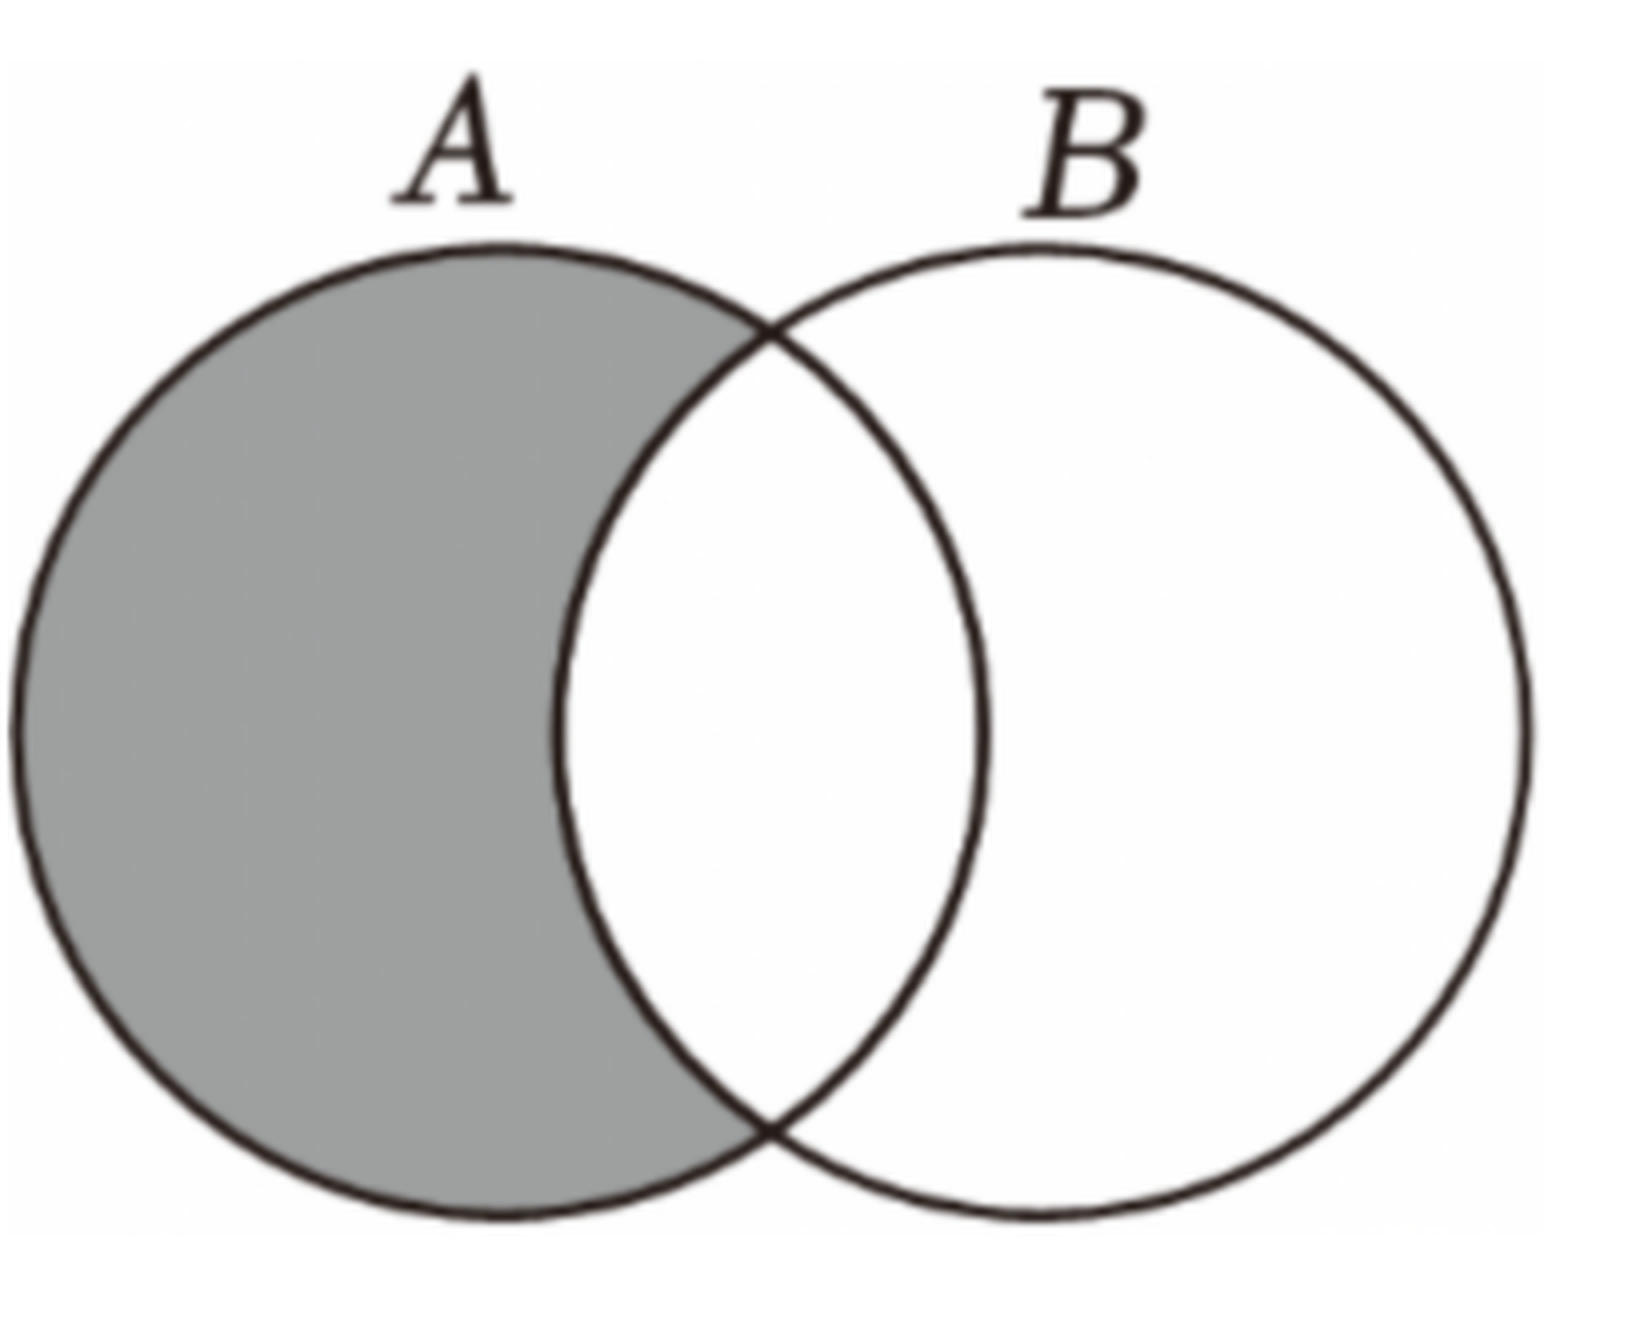
\includegraphics[width=0.30\textwidth]{figures/venn_A_minus_B_h38.png}
\end{center}

\ans{$\{1\}$}

\item 集合 $\{2,3,4,\cdots,2024,2025\}$ 的真子集的个数为 \blankline[4.4em].

\ans{$2^{2024}-1$}

\ifanswer
\solbegin
\step{集合 $\{2,3,4,\cdots,2024,2025\}$ 的真子集的个数为 $2^{2024}-1$.}
\solend

\fi

\item 已知集合 $A$ 中的元素都是正整数，其中最小的是 $1$，最大值是 $100$，除 $1$ 以外，每一个元
素都等于 $A$ 中的两个数（可以相同）的和，则集合 $A$ 中至少含有 \blankline[4.4em] 个元素.

\ans{$9$}

\ifanswer
\solbegin
\step{设 $A$ 中的数从小到大排列为 $1,a_1,a_2,\cdots,a_k,100$，}
\step{则 $a_1=1+1=2$；$3\leqslant a_2\leqslant 4$；$4\leqslant a_3\leqslant 8$；$5\leqslant a_4\leqslant 16$；$6\leqslant a_5\leqslant 32$；$7\leqslant a_6\leqslant 64$；}
\step{于是 $A$ 至少有八个数；}
\step{假设 $A$ 恰好有八个元素，由于 $a_5+a_6\leqslant 96<100$；}
\step{故必须有 $100=a_6+a_6$，$a_6=50$，}
\step{又 $a_4+a_5\leqslant 48$，同理 $a_5=25$，}
\step{但此时 $a_3+a_4\leqslant 24$，$a_5=2a_4$，$a_4=12.5$ 矛盾，}
\step{故 $A$ 不可能恰好有八个元素，因此 $A$ 至少有九个元素.}
\step{其九个数可以为 $1$，$2$，$3$，$6$，$12$，$13$，$25$，$50$，$100$.}
\solend

\fi

\item 已知集合 $\{x_1,x_2,x_3,x_4,x_5,x_6\}=\{1,2,3,4,5,6\}$，将 $x_i$ 与 $x_j$（其中 $i\in\{1,2,3\}$，
$j\in\{4,5,6\}$）的乘积 $x_ix_j$ 放入如图的 $3\times3$ 方格中，则方格中全部数之和的最大值为 \blankline[4.4em].

% 原卷的 $3\times3$ 方格是表格式内容（三行三列的公式），本稿按 高一03 的成例用 tabular 排出。
\begin{center}
\begin{tabular}{|c|c|c|}
\hline
$x_1x_4$ & $x_1x_5$ & $x_1x_6$ \\
\hline
$x_2x_4$ & $x_2x_5$ & $x_2x_6$ \\
\hline
$x_3x_4$ & $x_3x_5$ & $x_3x_6$ \\
\hline
\end{tabular}
\end{center}

\ans{$110$}

\ifanswer
\solbegin
\step{由表格数据得所有数之和为}
\step{$S=x_1x_4+x_1x_5+x_1x_6+x_2x_4+x_2x_5+x_2x_6+x_3x_4+x_3x_5+x_3x_6$，}
\step{所以 $S=(x_1+x_2+x_3)(x_4+x_5+x_6)$，}
\step{因为集合 $\{x_1,x_2,x_3,x_4,x_5,x_6\}=\{1,2,3,4,5,6\}$，}
\step{所以 $x_1+x_2+x_3+x_4+x_5+x_6=1+2+3+4+5+6=21$，}
\step{设 $t=x_1+x_2+x_3$，则 $6\leqslant t\leqslant 15$，$t\in\N^*$，}
\step{$S=t(21-t)=-\left(t-\dfrac{21}{2}\right)^2+\dfrac{441}{4}$，}
\step{当 $t=10$ 或 $t=11$ 时，$S=t(21-t)$ 取最大值，最大值为 $110$，}
\step{此时 $\{x_1,x_2,x_3\}=\{1,4,5\}$，$t=10$，所以可取最大值 $110$.}
\solend

\fi

\item 若 $[x]$ 表示不大于 $x$ 的最大整数，方程 $x^2-8[x]+7=0$ 的解集为 \blankline[4.4em].

\ans{$\{1,\sqrt{33},\sqrt{41},7\}$}

\ifanswer
\solbegin
\step{由题意，$x\geqslant[x]=\dfrac{x^2+7}{8}>0$，得 $x^2-8x+7\leqslant 0$，解得 $1\leqslant x\leqslant 7$，}
\step{$[x]=1$，$x^2=1$，$x=1$；}
\step{$[x]=2$，$x^2=9$，$x=3$ 与 $[x]=2$ 矛盾；}
\step{$[x]=3$，$x^2=17$，$x=\sqrt{17}$，$[x]=4$ 与 $[x]=3$ 矛盾；}
\step{$[x]=4$，$x^2=25$，$x=5$ 与 $[x]=4$ 矛盾；}
\step{$[x]=5$，$x^2=33$，$x=\sqrt{33}$，$[x]=5$；}
\step{$[x]=6$，$x^2=41$，$x=\sqrt{41}$，$[x]=6$；}
\step{$[x]=7$，$x^2=49$，$x=7$；}
\step{综上，方程 $x^2-8[x]+7=0$ 的解集为 $\{1,\sqrt{33},\sqrt{41},7\}$.}
\solend

\fi

\end{enumerate}

\bigsec{二、选择题}

\begin{enumerate}
\setcounter{enumi}{10}

\item 已知集合 $A=\{a,a^2\}$，$B=\{1,3\}$，若 $1\in A$，则 $A\cup B$ 中所有元素之和为\mbox{（\quad）}

\keepwithprev
A. $2$\qquad B. $3$\qquad C. $4$\qquad D. $5$

\ans{$B$}

\ifanswer
\solbegin
\step{因为 $1\in A$，集合 $A=\{a,a^2\}$，所以 $a=1$ 或 $a^2=1$，}
\step{若 $a=1$，则 $a=a^2$，与元素的互异性矛盾；}
\step{若 $a^2=1$，则 $a=1$（舍）或 $a=-1$，故 $A=\{-1,1\}$，$B=\{1,3\}$，}
\step{故 $A\cup B=\{-1,1,3\}$，所以 $A\cup B$ 中所有元素之和为 $-1+1+3=3$. 故选 $B$.}
\solend

\fi

\item 对于实数 $a$、$b$、$c$，下列命题正确的是\mbox{（\quad）}

\keepwithprev
A. 若 $a>b$，则 $ac^2>bc^2$\qquad B. 若 $a>b$，则 $a^2>b^2$

C. 若 $a>b$，则 $a|a|>b|b|$\qquad D. 若 $a>b>c>0$，则 $\dfrac{b}{a-b}<\dfrac{c}{a-c}$

\ans{$C$}

\ifanswer
\solbegin
\step{对于 $A$，若 $a>b$，$c=0$，则 $ac^2=bc^2$，故 $A$ 错误；}
\step{对于 $B$，若 $a>b$，取 $a=-1$，$b=-2$，则 $a^2<b^2$，故 $B$ 错误；}
\step{对于 $C$，若 $a>b>0$ 时，$a|a|-b|b|=a^2-b^2>0$，}
\step{当 $a>0>b$ 时，$a|a|-b|b|=a^2+b^2>0$，}
\step{当 $0>a>b$ 时，$a|a|-b|b|=b^2-a^2=(b-a)(b+a)>0$，}
\step{综上，若 $a>b$，则 $a|a|>b|b|$，故 $C$ 正确；}
\step{对于 $D$，若 $a>b>c>0$，$\dfrac{b}{a-b}-\dfrac{c}{a-c}=\dfrac{ab-bc-ac+bc}{(a-b)(a-c)}=\dfrac{a(b-c)}{(a-b)(a-c)}>0$，}
\step{故 $D$ 错误.}
\step{故选 $C$.}
\solend

\fi

\item 对于正整数集合 $A=\{a_1,a_2,\cdots,a_n\}(n\in\N^*,\ n\geqslant 3)$，如果去掉其中任意一个元素
$a_i(i=1,2,\cdots,n)$ 之后，剩余的所有元素组成的集合都能分为两个交集为空集的集合，且这
两个集合的所有元素之和相等，就称集合 $A$ 为平衡集. 记 $M=a_1+a_2+\cdots+a_n$. 若集合 $A$
是平衡集，并且存在 $a_i$ 为奇数，则集合 $A$ 中元素个数 $n$ 的奇偶性\mbox{（\quad）}

\keepwithprev
A. 与 $M$ 相关，既可以是奇数，又可以是偶数

B. 与 $M$ 无关，既可以是奇数，又可以是偶数

C. 与 $M$ 无关，必为偶数

D. 与 $M$ 无关，必为奇数

\ans{$D$}

\ifanswer
\solbegin
\step{正整数集合 $A=\{a_1,a_2,\cdots,a_n\}(n\in\N^*,\ n\geqslant 3)$，}
\step{因为集合 $A$ 是平衡集，设去掉元素 $a_i(i=1,2,\cdots,n)$，}
\step{由题意得 $A=A_1\cup A_2\cup\{a_i\}$，其中 $A_1\cap A_2=\varnothing$，}
\step{设集合 $A_1$ 和 $A_2$ 中的元素之和均为 $m$，所以 $M=2m+a_i$，其中 $i=1,2,\cdots,n$，}
\step{所以 $M-a_i=2m$，所以 $M-a_i$ 为偶数，其中 $i=1,2,\cdots,n$，}
\step{所以 $a_i(i=1,2,\cdots,n)$ 的奇偶性相同；}
\step{因为存在 $a_i$ 为奇数，所以 $a_i(i=1,2,\cdots,n)$ 均为奇数，}
\step{由 $M-a_i=2m$ 得 $M$ 也为奇数，且 $M=a_1+a_2+\cdots+a_n$，}
\step{所以 $n$ 也为奇数，所以 $n$ 必为奇数. 故选 $D$.}
\solend

\fi

\item 对于集合 $M=\{a\mid a=x^2-y^2,\ x\in\Z,\ y\in\Z\}$，给出如下三个结论：其中正确结论的个数
是\mbox{（\quad）}

\keepwithprev
①如果 $P=\{b\mid b=2n+1,\ n\in\Z\}$，那么 $P\sub M$；

②如果 $c=4n+2$，$n\in\Z$，那么 $c\notin M$；

③如果 $a_1\in M$，$a_2\in M$，那么 $a_1a_2\in M$.

\keepwithprev
A. $1$\qquad B. $2$\qquad C. $3$\qquad D. $0$

\ans{$C$}

\ifanswer
\solbegin
\step{对于①，$b=2n+1$，$n\in\Z$，则恒有 $2n+1=(n+1)^2-n^2$，}
\step{所以 $2n+1\in M$，即 $P=\{b\mid b=2n+1,n\in\Z\}$，则 $P\sub M$，①正确；}
\step{对于②，$c=4n+2$，$n\in\Z$，}
\step{若 $4n+2\in M$，则存在 $x$、$y\in\Z$ 使得 $x^2-y^2=4n+2$，}
\step{所以 $4n+2=(x+y)(x-y)$，又 $x+y$ 和 $x-y$ 同奇或同偶，}
\step{若 $x+y$ 和 $x-y$ 都是奇数，则 $(x+y)(x-y)$ 为奇数，而 $4n+2$ 是偶数；}
\step{若 $x+y$ 和 $x-y$ 都是偶数，则 $(x+y)(x-y)$ 能被 $4$ 整除，而 $4n+2$ 不能被 $4$ 整除，}
\step{所以 $4n+2\notin M$，即 $c\notin M$，②正确；}
\step{对于③，$a_1\in M$，$a_2\in M$，可设 $a_1=x_1^2-y_1^2$，$a_2=x_2^2-y_2^2$，$x_i$、$y_i\in\Z$；}
\step{则 $a_1a_2=(x_1^2-y_1^2)(x_2^2-y_2^2)=(x_1x_2)^2+(y_1y_2)^2-(x_1y_2)^2-(x_2y_1)^2$}
\step{$=(x_1x_2+y_1y_2)^2-(x_1y_2+x_2y_1)^2\in M$，那么 $a_1a_2\in M$，③正确.}
\step{综上，正确的命题是①②③. 故选 $C$.}
\solend

\fi

\end{enumerate}

\bigsec{三、解答题}

\begin{enumerate}
\setcounter{enumi}{14}

\item 已知 $A=\{x\mid a\leqslant x\leqslant -a+3\}$，$B=\{x\mid x<-1\text{ 或 }x>5\}$.

\begin{enumerate}[label=(\arabic*)]

\item 若 $A\cap B=\varnothing$，求 $a$ 的取值范围；

\item 若 $A\cup B=\R$，求 $a$ 的取值范围.

\end{enumerate}

\ans{（1）$[-1,+\infty)$；（2）$(-\infty,-2]$}

\ifanswer
\solbegin
\stepm{(1)}{①当 $A=\varnothing$ 时，$A\cap B=\varnothing$，需满足 $a>-a+3$，解得 $a>\dfrac32$，}
\step{故 $a$ 的取值范围为 $\left(\dfrac32,+\infty\right)$.}
\step{②当 $A\neq\varnothing$ 时，要使 $A\cap B=\varnothing$，需满足
$\begin{cases}a\leqslant\dfrac32\\[4pt] -a+3\leqslant 5\\[4pt] a\geqslant -1\end{cases}$，解得 $-1\leqslant a\leqslant\dfrac32$.}
\step{综上所述，$a$ 的取值范围是 $[-1,+\infty)$.}
\stepm{(2)}{因为 $A\cup B=\R$，$A=\{x\mid a\leqslant x\leqslant -a+3\}$，$B=\{x\mid x<-1\text{ 或 }x>5\}$，}
\step{所以 $\begin{cases}-a+3\geqslant 5\\[4pt] a\leqslant -1\end{cases}$，解得 $a\leqslant -2$，故所求 $a$ 的取值范围为 $(-\infty,-2]$.}
\solend

\fi

\ansspace[6]

\item 已知集合 $A=\{x\mid mx^2+x-2=0\}$，$B=\{x\mid 2x^2-5x-12=0\}$.

\begin{enumerate}[label=(\arabic*)]

\item 若 $A$ 中有且仅有 $1$ 个元素，求实数 $m$ 的值；

\item 已知集合 $C=A\cup B$，若 $C$ 的真子集有且仅有 $3$ 个，求实数 $m$ 的取值范围.

\end{enumerate}

\ans{（1）$m=0$ 或 $m=-\dfrac18$；（2）$\left\{m\mid m\leqslant -\dfrac18\right\}$}

\ifanswer
\solbegin
\stepm{(1)}{若 $m=0$，方程化为 $x-2=0$，此时方程有且仅有一个根 $x=2$；}
\step{若 $m\neq 0$，则 $\Delta=1^2-4\times m\times(-2)=0$，即 $m=-\dfrac18$ 时，}
\step{方程有两个相等的实根，此时集合 $A$ 中有且仅有一个元素，}
\step{所以实数 $m$ 的值为 $m=0$ 或 $m=-\dfrac18$；}
\stepm{(2)}{$B=\{x\mid 2x^2-5x-12=0\}=\left\{-\dfrac32,4\right\}$，}
\step{因为 $C=A\cup B$，若 $C$ 的真子集有且仅有 $3$ 个，则 $C$ 中有两个元素，}
\step{所以 $A\sub B$，由（1）得 $m=0$ 时，$A=\{2\}$，不符合 $A\sub B$，}
\step{当 $m\neq 0$ 时，若 $\Delta=1^2-4\times m\times(-2)<0$，解得 $m<-\dfrac18$，}
\step{此时 $A=\varnothing$，符合 $A\sub B$，}
\step{若 $\Delta=1^2-4\times m\times(-2)=0$，解得 $m=-\dfrac18$，}
\step{此时方程 $mx^2+x-2=0$ 的根为 $x=4$，集合 $A=\{4\}$，符合 $A\sub B$，}
\step{若 $\Delta=1^2-4\times m\times(-2)>0$，由 $A\sub B$，得 $A=\left\{-\dfrac32,4\right\}$，}
\step{此时有 $-\dfrac32+4=-\dfrac1m$ 且 $-\dfrac32\times 4=-\dfrac2m$，无解，}
\step{综上所述，实数 $m$ 的取值范围为 $\left\{m\mid m\leqslant -\dfrac18\right\}$.}
\solend

\fi

\ansspace[6]

\item 设 $A$ 是非空实数集，且 $0\notin A$. 若对于任意的 $x$、$y\in A$，都有 $xy\in A$，则称集合 $A$ 具
有性质 $P_1$；若对于任意的 $x$、$y\in A$，都有 $\dfrac xy\in A$，则称集合 $A$ 具有性质 $P_2$.

\begin{enumerate}[label=(\arabic*)]

\item 写出一个恰含有两个元素且具有性质 $P_1$ 的集合 $A$，并说明理由；

\item 证明：“非空实数集 $A$ 具有性质 $P_1$”是“非空实数集 $A$ 具有性质 $P_2$”的必要非充分条
件.

\end{enumerate}

\ans{（1）$A=\{-1,1\}$，理由见解析；（2）见解析}

\ifanswer
\solbegin
% 注：原卷本题 (1) 的解析里“证明”一词重复出现两次（一次接在分号后、一次另起一行），
%     本稿照原卷重复录入，未去重。
\stepm{(1)}{$A=\{-1,1\}$，证明：恰含有两个元素且具有性质 $P_1$ 的集合 $A=\{-1,1\}$；}
\step{证明：$1\times 1=1\in A$，$1\times(-1)=-1\in A$，$-1\times 1=-1\in A$，$-1\times(-1)=1\in A$；}
\stepm{(2)}{若集合 $A$ 具有性质 $P_2$，不妨设 $a\in A$，}
\step{由非空数集 $A$ 具有性质 $P_2$，有 $\dfrac aa=1\in A$.}
\step{①$A=\{1\}$，易得此时集合 $A$ 具有性质 $P_1$.}
\step{②数集 $A$ 只含有两个元素，不妨设 $A=\{1,a_1\}$，}
\step{由 $\dfrac{1}{a_1}=a_1$，且 $a_1\neq 1$，解得 $a_1=-1$，此时集合 $A$ 具有性质 $P_1$.}
\step{③实数集 $A$ 含有两个以上的元素，不妨设不为 $1$ 的元素 $a_1$、$a_2\in A$，}
\step{则有 $\dfrac{1}{a_1}\in A$，由于集合 $A$ 具有性质 $P_2$，}
\step{所以有 $a_2\div\dfrac{1}{a_1}=a_1a_2\in A$，这说明集合 $A$ 具有性质 $P_1$.}
\step{综上，若非空实数集 $A$ 具有性质 $P_2$，则集合 $A$ 具有性质 $P_1$，}
\step{所以“非空实数集 $A$ 具有性质 $P_1$”是“非空实数集 $A$ 具有性质 $P_2$”的}
\step{必要条件.}
\step{取正偶数集 $A=\{x\mid x=2n,\ n\in\N^*\}$，}
\step{对任意的 $2m$、$2n\in A$，$m$、$n\in\N^*$，}
\step{有 $2m\times 2n=4mn\in A$，故 $A$ 具有性质 $P_1$，}
\step{取 $x=2$，$y=4$，则 $\dfrac xy=\dfrac12\notin A$，故 $A$ 不具有性质 $P_2$，}
\step{所以“非空实数集 $A$ 具有性质 $P_1$”不是“非空实数集 $A$ 具有性质 $P_2$”的}
\step{充分条件.}
\step{综上，“非空实数集 $A$ 具有性质 $P_1$”是“非空实数集 $A$ 具有性质 $P_2$”的}
\step{必要非充分条件.}
\solend

\fi

\ansspace[8]

\item 已知命题 $p$：关于 $x$ 的方程 $x^2+mx+1=0$ 有两个不同的正根；命题 $q$：关于 $x$ 的方程
$4x^2+4(m-2)x=-1$ 有实根.

\begin{enumerate}[label=(\arabic*)]

\item 若命题 $q$ 为假命题，求整数 $m$ 的解集；

\item 若命题 $p$ 为真命题，且关于 $x$ 的方程 $x^2+mx+1=0$ 的两个实数根 $x_1$、$x_2$ 满足
$3x_1+2x_2=5$，求实数 $m$ 的取值集合；

\item 若命题 $p$ 和命题 $q$ 有且仅有一个成立，求实数 $m$ 的取值范围.

\end{enumerate}

\ans{（1）$\{2\}$；（2）$\left\{-\dfrac{13}{6}\right\}$；（3）$[-2,1]\cup[3,+\infty)$}

\ifanswer
\solbegin
\stepm{(1)}{命题 $q$：关于 $x$ 的方程 $4x^2+4(m-2)x=-1$ 有实根为假命题，}
\step{即 $4x^2+4(m-2)x+1=0$ 无实根，}
\step{则 $\Delta=16(m-2)^2-16<0$，则 $1<m<3$，则整数 $m$ 的解集为 $\{2\}$；}
\stepm{(2)}{若命题 $p$ 为真命题，且关于 $x$ 的方程 $x^2+mx+1=0$ 的两个实数根 $x_1$、$x_2$，}
\step{满足 $3x_1+2x_2=5$，则方程 $x^2+mx+1=0$ 有两个不同的正根，}
\step{则 $\begin{cases}\Delta=m^2-4>0\\[4pt] x_1+x_2=-m>0\end{cases}$，则 $m<-2$，}
\step{又 $\begin{cases}x_1+x_2=-m\\[4pt] x_1x_2=1\\[4pt] 3x_1+2x_2=5\end{cases}$，
则 $\begin{cases}x_1=5+2m\\[4pt] x_2=-3m-5\end{cases}$，则 $(5+2m)(-3m-5)=1$，}
\step{得 $m=-2$ 或 $m=-\dfrac{13}{6}$，又因为 $m<-2$，所以 $m=-\dfrac{13}{6}$，}
\step{所以实数 $m$ 的取值集合为 $\left\{-\dfrac{13}{6}\right\}$；}
\stepm{(3)}{由（2）得当 $p$ 为真时，则有 $m<-2$，}
\step{当 $q$ 为真时，$\Delta=16(m-2)^2-16\geqslant 0$，解得 $m\leqslant 1$ 或 $m\geqslant 3$，}
\step{又因为命题 $p$ 和命题 $q$ 只有一个为真，所以
$\begin{cases}m<-2\\[4pt] 1<m<3\end{cases}$ 或 $\begin{cases}m\geqslant -2\\[4pt] m\leqslant 1\text{ 或 }m\geqslant 3\end{cases}$，}
\step{解得 $-2\leqslant m\leqslant 1$ 或 $m\geqslant 3$，所以实数 $m$ 的取值范围为 $[-2,1]\cup[3,+\infty)$.}
\solend

\fi

\ansspace[8]

% 注：原卷此处作“设 $n\in\N^*$，集合含有 $3n$ 个元素”，**漏了符号 $U$**（应作“集合 $U$
%     含有 $3n$ 个元素”）——$U$ 直到本句末尾“则称 $U$ 为三分集合”才出现、此前无定义。
%     本稿照录未补，见文件头“原卷笔误/存疑”⑦。
\item 设 $n\in\N^*$，集合含有 $3n$ 个元素，若存在三个 $n$ 元集合 $A$、$B$、$C$ 满足如下两个条件，
则称 $U$ 为三分集合.

①$U=A\cup B\cup C$；

②$A$、$B$、$C$ 元素可分别排列为有序数组 $(a_1,a_2,\cdots,a_n)$，$(b_1,b_2,\cdots,b_n)$ 及
$(c_1,c_2,\cdots,c_n)$，使得对 $\forall i=1,2,\cdots,n$，均有 $a_i+b_i=c_i$.

特别地，当 $U=\{1,2,3,4,\cdots,3n-2,3n-1,3n\}$ 为三分集合时，称 $n$ 为完美三分数.

如：因为 $U=\{1,2,3\}$ 为三分集合，所以 $n=1$ 为最小完美三分数.

\begin{enumerate}[label=(\arabic*)]

\item 请判断下列两个集合是否为三分集合（直接写出结论）：

$U_1=\{1,2,3,4,5,6\}$，$U_2=\{1,3,5,7,8,9,10,11,12\}$；

\item 求出大于 $1$ 的最小完美三分数；

\item 请判断是否存在无穷多个完美三分数？若存在，请说明理由；若不存在，则求出最大的
完美三分数.

\end{enumerate}

\ans{（1）$U_1$ 不是三分集合，$U_2$ 是三分集合；（2）$4$；（3）存在，理由见解析}

\ifanswer
\solbegin
\stepm{(1)}{(i)$U_1=\{1,2,3,4,5,6\}$ 不是三分集合，下面用反证法证明：}
\step{证明：假设 $U=\{1,2,3,4,5,6\}$ 是三分集合，}
\step{设 $A=\{a_1,a_2\}$，$B=\{b_1,b_2\}$，$C=\{c_1,c_2\}$，不妨设 $c_1<c_2$，}
\step{因为 $a_1+b_1=c_1$，$a_2+b_2=c_2$，}
\step{所以 $a_1+b_1+a_2+b_2+c_1+c_2=2(c_1+c_2)=1+2+3+4+5+6=21$，}
% 注：原卷此步印“所以 $c_1+c_2=2$”，与上一行的 $2(c_1+c_2)=21$ **不自洽**
%     （应作 $\dfrac{21}2$）；同题 $n=3$ 处的同型推理原卷写的是 $\dfrac{45}2$，故此处是原卷笔误。
%     本稿照录未改，见文件头“原卷笔误/存疑”⑧。
\step{所以 $c_1+c_2=2$，这与 $c_1,c_2\in\N^*$ 矛盾，故假设错误，}
\step{故 $U_1=\{1,2,3,4,5,6\}$ 不是三分集合；}
\step{(ii)$U_2=\{1,3,5,7,8,9,10,11,12\}$ 是三分集合，理由如下：}
\step{令 $A=\{1,3,5\}$，$B=\{9,8,7\}$，$C=\{10,11,12\}$，}
\step{则 $A\cup B\cup C=U=\{1,3,5,7,8,9,10,11,12\}$，满足条件①；}
\step{又 $1+9=10$；$3+8=11$；$5+7=12$，所以满足条件②，}
\step{所以 $U_2=\{1,3,5,7,8,9,10,11,12\}$ 是三分集合；}
\stepm{(2)}{由（1）得，当 $n=2$ 时，$U=\{1,2,3,4,5,6\}$ 不是三分集合；}
\step{当 $n=3$ 时，$U=\{1,2,3,4,5,6,7,8,9\}$，}
\step{假设 $U=\{1,2,3,4,5,6,7,8,9\}$ 是三分集合，}
\step{同理由 $a_1+b_1+a_2+b_2+a_3+b_3+c_1+c_2+c_3$}
\step{$=2(c_1+c_2+c_3)=1+2+\cdots+9=45$，$c_1+c_2+c_3=\dfrac{45}{2}$，}
\step{可推出与 $c_1$、$c_2$、$c_3\in\N^*$ 矛盾，故假设也错误，}
\step{所以 $U=\{1,2,3,4,5,6,7,8,9\}$ 不是三分集合；}
\step{当 $n=4$ 时，$U=\{1,2,3,\cdots,12\}$，}
\step{存在三个 $4$ 元集合 $A=\{1,2,4,3\}$，$B=\{5,8,7,9\}$，$C=\{6,10,11,12\}$，}
\step{满足 $U=\{1,2,3,\cdots,12\}$ 为三分集合的两个条件，}
\step{故大于 $1$ 的最小完美三分数为 $4$；}
\stepm{(3)}{存在无穷多个完美三分数，理由如下：}
\step{由题意得，$n=1$ 为最小完美三分数，}
\step{当 $n=5$ 时，$U=\{1,2,3,\cdots,15\}$，}
\step{存在三个 $5$ 元集合 $A=\{1,3,5,7,2\}$，$B=\{11,10,9,8,4\}$，$C=\{12,13,14,15,6\}$，}
\step{满足三分集合的条件，故 $5$ 为完美三分数；}
\step{当 $n=21$ 时，$U=\{1,2,3,\cdots,63\}$，}
\step{存在如下三个 $21$ 元的集合满足三分集合的条件：}
\step{$A=\{1,3,5,7,\cdots,29,31,2,6,10,14,4\}$，}
\step{$B=\{47,46,45,44,\cdots,33,32,22,20,18,16,8\}$，}
\step{$C=\{48,49,50,51,\cdots,62,63,24,26,28,30,12\}$，}
\step{故 $21$ 为完美三分数.}
\step{首先证明：若 $n=k$，$k\in\N^*$ 为三分完美数，}
\step{则 $n=4k+1$，$k\in\N^*$ 也为三分完美数，}
% 注：下一行原卷印作“$U_{k+1}=U_{k+1}=\{2,3,\cdots,12k+3\}$”——等号两边记号相同，
%     依上下文疑当作 $U'_{k+1}=U_{4k+1}$，且此处集合自 2 起（前文 $U_{4k+1}$ 自 1 起）；
%     本稿照录原卷，未代为改写。
\step{证明：记 $U_k=\{1,2,3,\cdots,3k\}$，$U_{4k+1}=\{1,2,3,\cdots,12k+3\}$，}
\step{若 $n=k$，$k\in\N^*$ 为三分完美数，则 $U_k$ 为三分集合，}
\step{即存在三个 $k$ 元集合 $A$、$B$、$C$ 满足如下两个条件，}
\step{①$U_k=A\cup B\cup C$；}
\step{②$A$、$B$、$C$ 元素可分别排列为有序数组 $(a_1,a_2,\cdots,a_k)$，}
\step{$(b_1,b_2,\cdots,b_k)$ 及 $(c_1,c_2,\cdots,c_k)$，}
\step{使得对 $\forall i=1,2,3,\cdots,k$，均有 $a_i+b_i=c_i$，}
\step{则可得到对 $\forall i=1,2,3,\cdots,k$，$2a_i+2b_i=2c_i$，}
\step{故集合 $\{2,4,6,\cdots,6k\}$ 也满足三分集合的两个条件，其也为三分集合，}
\step{下面记集合 $\{2,4,6,\cdots,6k\}=2U_k$，}
\step{对 $n=4k+1$，集合 $U_{k+1}=U_{k+1}=\{2,3,\cdots,12k+3\}=(2U_k)\cup\complement_{U_{4k+1}}(2U_k)$，}
\step{构造集合 $A'=\{1,3,5,7,\cdots,6k+1\}$，共有 $3k+1$ 个奇数；}
% 注：下一行原卷印作“$B'=\{6k+3k+2,6k+3k+1,6k+3k,6k+3k-1,\cdots,6k+2\}$”，
%     按与后文 $C'$ 相接，前四项当写作 $9k+2$、$9k+1$、$9k$、$9k-1$；本稿照录原卷。
\step{集合 $B'=\{6k+3k+2,6k+3k+1,6k+3k,6k+3k-1,\cdots,6k+2\}$，}
\step{共有 $3k+1$ 个逐个减小的连续正整数；}
\step{集合 $C'=\{9k+3,9k+4,9k+5,9k+6,\cdots,12k+3\}$，}
\step{共有 $3k+1$ 个逐个增大的连续正整数；}
\step{得这三个 $3k+1$ 元集合 $A'$、$B'$、$C'$ 满足如下两个条件，}
\step{①集合 $A'\cup B'\cup C'=\complement_{U_{4k+1}}(2U_k)$；}
\step{②$A'$、$B'$、$C'$ 元素可分别排列为有序数组 $(a_1,a_2,\cdots,a_{3k+1})$，}
\step{$(b_1,b_2,\cdots,b_{3k+1})$ 及 $(c_1,c_2,\cdots,c_{3k+1})$，}
\step{使得对 $\forall i=1,2,3,\cdots,3k+1$，均有 $a_i+b_i=c_i$；}
\step{故 $\complement_{U_{4k+1}}(2U_k)$ 为三分集合，而已知 $U_k$ 为三分集合，}
\step{将其对应与 $A'$、$B'$、$C'$ 合并，}
% 注：原卷此处印“令 $A''=A\cup A'$”（$B''$、$C''$ 同）。按同段上文“记集合
%     $\{2,4,6,\cdots,6k\}=2U_k$”，此处疑当作 $A''=2A\cup A'$——否则
%     $A''\cup B''\cup C''=U_k\cup\complement_{U_{4k+1}}(2U_k)\neq U_{4k+1}$，与本段结论冲突。
%     本稿照录未改，见文件头“原卷笔误/存疑”⑨。
\step{令 $A''=A\cup A'$，$B''=B\cup B'$，$C''=C\cup C'$，}
\step{则这三个 $4k+1$ 元集合 $A''$、$B''$、$C''$，}
\step{满足 $A''\cup B''\cup C''=U_{4k+1}$，且满足条件②，}
\step{故 $U_{4k+1}=\{1,2,3,\cdots,12k+3\}$ 为三分集合，}
\step{因此可得，若 $n=k$ 为三分完美数，则 $n=4k+1$ 也为三分完美数，}
\step{由 $1$，$5$，$21$ 为完美三分数，结合所证结论得，存在无穷多个完美三分数.}
\solend

\fi

\ansspace*[12]

\end{enumerate}

\end{document}
"
% 紧凑版：xelatex "\def\iscompact{1}% 高一38_大同中学_周末作业3.tex
%   —— 高一上数学“2026-2027 年大同中学高一上周末作业 3”（试卷版/答案版）
% 试卷版：xelatex 高一38_大同中学_周末作业3.tex
% 答案版：xelatex "\def\isanswer{1}\input{高一38_大同中学_周末作业3.tex}"
% 紧凑版：xelatex "\def\iscompact{1}\input{高一38_大同中学_周末作业3.tex}"
%
% 原始材料是微信公众号图文（公众号“魔都数学加油站”连载“27学年高一 38”，署名“破晓”，
% 2026-09-26 21:29 发布，原文标题“27学年高一38——2026-2027年上海市大同中学高一上周末作业3”，
% 原文链接 https://mp.weixin.qq.com/s/O_O60vCIiGi2xponAo4irw ），正文为 12 张 PNG 页。
% **同一篇里各页分辨率不一致**（2560×3620 与 4762×6735 两档混排：第 1、10、11、12 页为
% 2560×3620，第 2—9 页为 4762×6735）。原文本身就是一份**讲评版**——有的题下方只印
% 【答案】行，有的只印【解析】。试题文字、答案与解析均照原卷录入，未改内容。卷面的粉色
% 斜水印“魔都数学加油站”属水印，未录入。
%
% 本卷共 **17 题**：填空题 8 题（第 3—10 题）、选择题 4 题（第 11—14 题）、解答题 5 题
% （第 15—19 题）；插图 1 张（第 6 题 Venn 图）。三版页数：试卷版 4 页 / 答案版 11 页 /
% 紧凑版 3 页，`Overfull`／`Underfull`／`Missing character` 告警均为 0。
%
% 卷首标题：原卷印作“2026-2027 年大同中学高一上周末作业 3”（公众号原文标题里的“上海市”
% 三字卷面标题行没有，本稿照卷面），年份区间按全稿惯例排 en dash，前缀照原卷保留“年”。
%
% 与原卷的排版差异（均已在 README“说明”中交代）：
%   ① 原文自**第 3 题**起（第 1、2 题未在该文中发布），故本稿题号亦自 3 起，填空题以
%      \setcounter{enumi}{2} 起编；选择、解答两节各按上一节末号另设 \setcounter
%      （选择题 \setcounter{enumi}{10}、解答题 \setcounter{enumi}{14}）；
%   ② 原卷本就印有“一、填空题”“二、选择题”“三、解答题”三节标题，本稿照原卷分节，
%      只把标题改排成全稿统一的“大节标题”样式；
%   ③ 原卷是“讲评版”：第 3、6 题只印【答案】行，第 4、5、7、8、9、10 题与第 11—19 题印
%      【解析】；本稿统一改为试卷版隐去、答案版以 \ans{}／\ifanswer 块给出，两版彻底分离。
%      其中第 4、5、7、8、9、10 题与第 11—14 题的答案，原卷写在【解析】末句，本稿另提为
%      \ans{}；第 15—19 题原卷只有【解析】、无独立答案行，本稿亦补了摘要式 \ans{}。
%      **故本卷 17 题每题都有 \ans**——比“只印【解析】的填空、解答题不另提 \ans”的
%      高一31／高一34 更彻底，与 高一21 第 11 题（填空，答案在【解析】末句，本稿另提）同类；
%      （本仓对“另提 \ans{}”的做法各卷不一，见 README 对应专记的核对面。）
%   ④ 数集记号原卷两套并用：第 3、5 题的实数集作粗体 $\mathbf{R}$，第 8、14、17、18 题等的
%      整数集、自然数集作斜体 $Z$、$N$，本稿按全稿惯例统一写作 $\R$、$\Z$、$\N$；
%   ⑤ 原卷填空的横线宽度不一（约 1.8—3.6 字宽），本稿按全稿惯例统一排 \blankline[4.4em]；
%   ⑥ 中文括注原卷用半角“(  )”，本稿按全稿惯例排全角；选择题的作答括注统一排
%      \mbox{（\quad）}（第 14 题的作答括注原卷印在 ①②③ 三个命题**之前**，本稿照原卷次序）；
%      数学式内部的括注（如第 4 题的 $p\%(0<p<100)$、第 13 题的 $a_i(i=1,2,\cdots,n)$）照原样
%      留在行内公式里，未改全角；
%   ⑦ 原卷并列的字母（“x,y”“a,b,c”）不加标点或作半角逗号，本稿按全稿惯例改排顿号；
%   ⑧ 第 6 题的 Venn 图取原卷截图、4× LANCZOS 放大（figures/venn_A_minus_B_h38.png，
%      见该处 \includegraphics 前的注释）；第 9 题的 $3\times3$ 方格属**表格式**内容，
%      本稿按 高一03 的成例用 tabular 排出，未截图；
%   ⑨ 原卷未印副标题，本稿按**本卷实际内容**补出副标题“集合与常用逻辑用语”（依据见下条）；
%   ⑩ 原卷【解析】**一个印刷行照录为一条 `\step`**（原卷的折行也照录为独立一条，如第 17 题
%      末三处“…的”／“必要条件.”这类跨行句、第 9 题“由表格数据得所有数之和为”／
%      “$S=\cdots$，”），使答案版的排布与原卷讲评版逐行对应；全卷 15 处【解析】合计
%      **191 条 `\step` ＝ 原卷 191 行**（逐处：5、5、1、9、9、9、4、9、9、12、6、14、21、13、65）。
%
% 副标题（\examtitlest 第二个参数）：本卷卷面未印副标题，由本稿补出，取值按 2026-09-26 起的
%   新口径“只用本卷实际内容的模块名”定为“集合与常用逻辑用语”。依据：全卷 17 题
%   （第 3—19 题）中，第 3、5、6、7、8、9、10、11、13、14、15、16、17、18、19 题共 15 题
%   是集合的运算与关系、子集计数、集合新定义（性质 $P_1$／$P_2$、平衡集、三分集合），以及
%   命题与逻辑（第 3 题即用反证法证明“$x+y>2\Rightarrow x>1$ 或 $y>1$”这一命题）；不等式只
%   出现在第 4 题（降价提价的应用比较）、第 12 题（不等式命题真假）与第 10 题解析里解一元
%   二次不等式，合计不足全卷的三分之一，故不并标“不等式”。
%
% 原卷笔误/存疑（均照抄原卷、未改，见源码中该处上方注释）：
%   ① 第 19 题 (3) 的证明里印作“集合 $U_{k+1}=U_{k+1}=\{2,3,\cdots,12k+3\}$”——等号两边
%      记号相同（依上下文疑当作 $U'_{k+1}=U_{4k+1}$），且此处集合自 $2$ 起，而前文
%      $U_{4k+1}=\{1,2,3,\cdots,12k+3\}$ 自 $1$ 起；本稿照录；
%   ② 第 19 题 (3) 的证明里印作
%      “$B'=\{6k+3k+2,6k+3k+1,6k+3k,6k+3k-1,\cdots,6k+2\}$”——按与后文
%      $C'=\{9k+3,9k+4,9k+5,9k+6,\cdots,12k+3\}$ 相接，前四项当写作 $9k+2$、$9k+1$、
%      $9k$、$9k-1$（即 $6k+3k+2$ 等），原卷即作“$6k+3k+\cdots$”形式，本稿照录；
%   ③ 第 19 题的术语前后不一：题干与 (1)(2)(3) 用“完美三分数”，而 (3) 的证明里五次写作
%      “三分完美数”（词序不同）；本稿五处都照录；
%   ④ 第 14 题题干作“给出如下三个结论：其中正确结论的个数是（\quad）”，此处冒号疑当作
%      逗号，本稿照录；
%   ⑤ 第 17 题题干作“非空实数集”，其解析有一处写作“非空数集”；本稿照录；
%   ⑥ 第 17 题 (1) 的【解析】原卷连写“…集合 $A=\{-1,1\}$；证明：…；证明：…”，“证明”
%      一词重复出现两次（第一次在分行处、第二次另起一行），本稿照原卷重复录入，未去重。
%   ⑦ 第 19 题**题干漏字**：原卷作“19.设 $n\in\N^*$，集合含有 $3n$ 个元素…则称 $U$ 为
%      三分集合”——首句漏了符号 $U$（应作“集合 $U$ 含有 $3n$ 个元素”），$U$ 直到结论句
%      才出现、此前无定义；本稿照录未补（见该处上方注释）。
%   ⑧ 第 19(1)(i) 的【解析】**自相矛盾**：上一行印“$a_1+b_1+a_2+b_2+c_1+c_2=2(c_1+c_2)
%      =1+2+3+4+5+6=21$”，下一行却印“所以 $c_1+c_2=2$”（由 $2(c_1+c_2)=21$ 应得
%      $c_1+c_2=\dfrac{21}2$，非整数、才与 $c_1,c_2\in\N^*$ 矛盾）；同题 $n=3$ 处的同型
%      推理原卷就写对了（$\dfrac{45}2$），故此处是原卷笔误；本稿照录未改（见该处上方注释）。
%   ⑨ 第 19(3) 的【解析】印“令 $A''=A\cup A'$，$B''=B\cup B'$，$C''=C\cup C'$”——按同段
%      上文“记集合 $\{2,4,6,\cdots,6k\}=2U_k$”，$A''$ 等疑当作 $2A\cup A'$（$B''$、$C''$ 同），
%      否则 $A''\cup B''\cup C''=U_k\cup\complement_{U_{4k+1}}(2U_k)\neq U_{4k+1}$；本稿照录未改
%      （见该处上方注释）。

\documentclass[a4paper,11pt]{article}
\usepackage{common}

\begin{document}

\examtitlest[3]{2026--2027 年大同中学高一上周末作业 3}{集合与常用逻辑用语}

\bigsec{一、填空题}

\begin{enumerate}
% 原卷填空题自第 3 题起（第 1、2 题未在该文中发布），须与选择、解答两节的 \setcounter 对齐
\setcounter{enumi}{2}

\item 设 $x$、$y\in\R$，若 $x+y>2$，则 $x>1$ 或 $y>1$ 是真命题. 这个命题可以用反证法去证明，
可以假设：\blankline[4.4em].

\ans{$x\leqslant 1$ 且 $y\leqslant 1$}

\item 已知某商品的原价为 $a$ 元，由于市场原因，先降价 $p\%(0<p<100)$ 出售，一段时间后，
再提价 $p\%$ 出售，则该商品提价后的售价 \blankline[4.4em] 该商品的原价（填“高于”“低于”或“等于”）.

\ans{低于}

\ifanswer
\solbegin
\step{由题意得第一次降价后的售价为 $a(1-p\%)$ 元，}
\step{第二次提价后的售价为 $a(1-p\%)(1+p\%)$ 元，}
\step{因为 $0<p<100$，所以 $0<p\%<1$，}
\step{因为 $a(1-p\%)(1+p\%)=a[1-(p\%)^2]<a$，}
\step{即该商品提价后的售价低于该商品的原价.}
\solend

\fi

\item 若集合 $A=\{x\mid ax^2+ax+1=0,\ a\in\R,\ x\in\R\}$ 的子集只有两个，则实数 $a=$ \blankline[4.4em].

\ans{$4$}

\ifanswer
\solbegin
\step{集合 $A=\{x\mid ax^2+ax+1=0\}$ 的子集只有两个，}
\step{所以 $A$ 有且只有一个元素，}
\step{①若 $a=0$，则 $A=\varnothing$ 不成立；}
\step{②若 $a\neq 0$，则 $\Delta=a^2-4a=0$，解得 $a=4$（$0$ 舍）.}
\step{故 $a=4$.}
\solend

\fi

\item 如图，已知集合 $A=\{1,2,3,4,5\}$，集合 $B=\{2,3,4,5,9\}$，则图中阴影部分所表示的
集合为 \blankline[4.4em].

% 图取原卷截图（01.png，2560×3620）右栏，4× LANCZOS 放大；为避免与 高一11 的
% figures/venn_A_minus_B.png 同名，按 高一32 的成例加 _h38 后缀。
\begin{center}
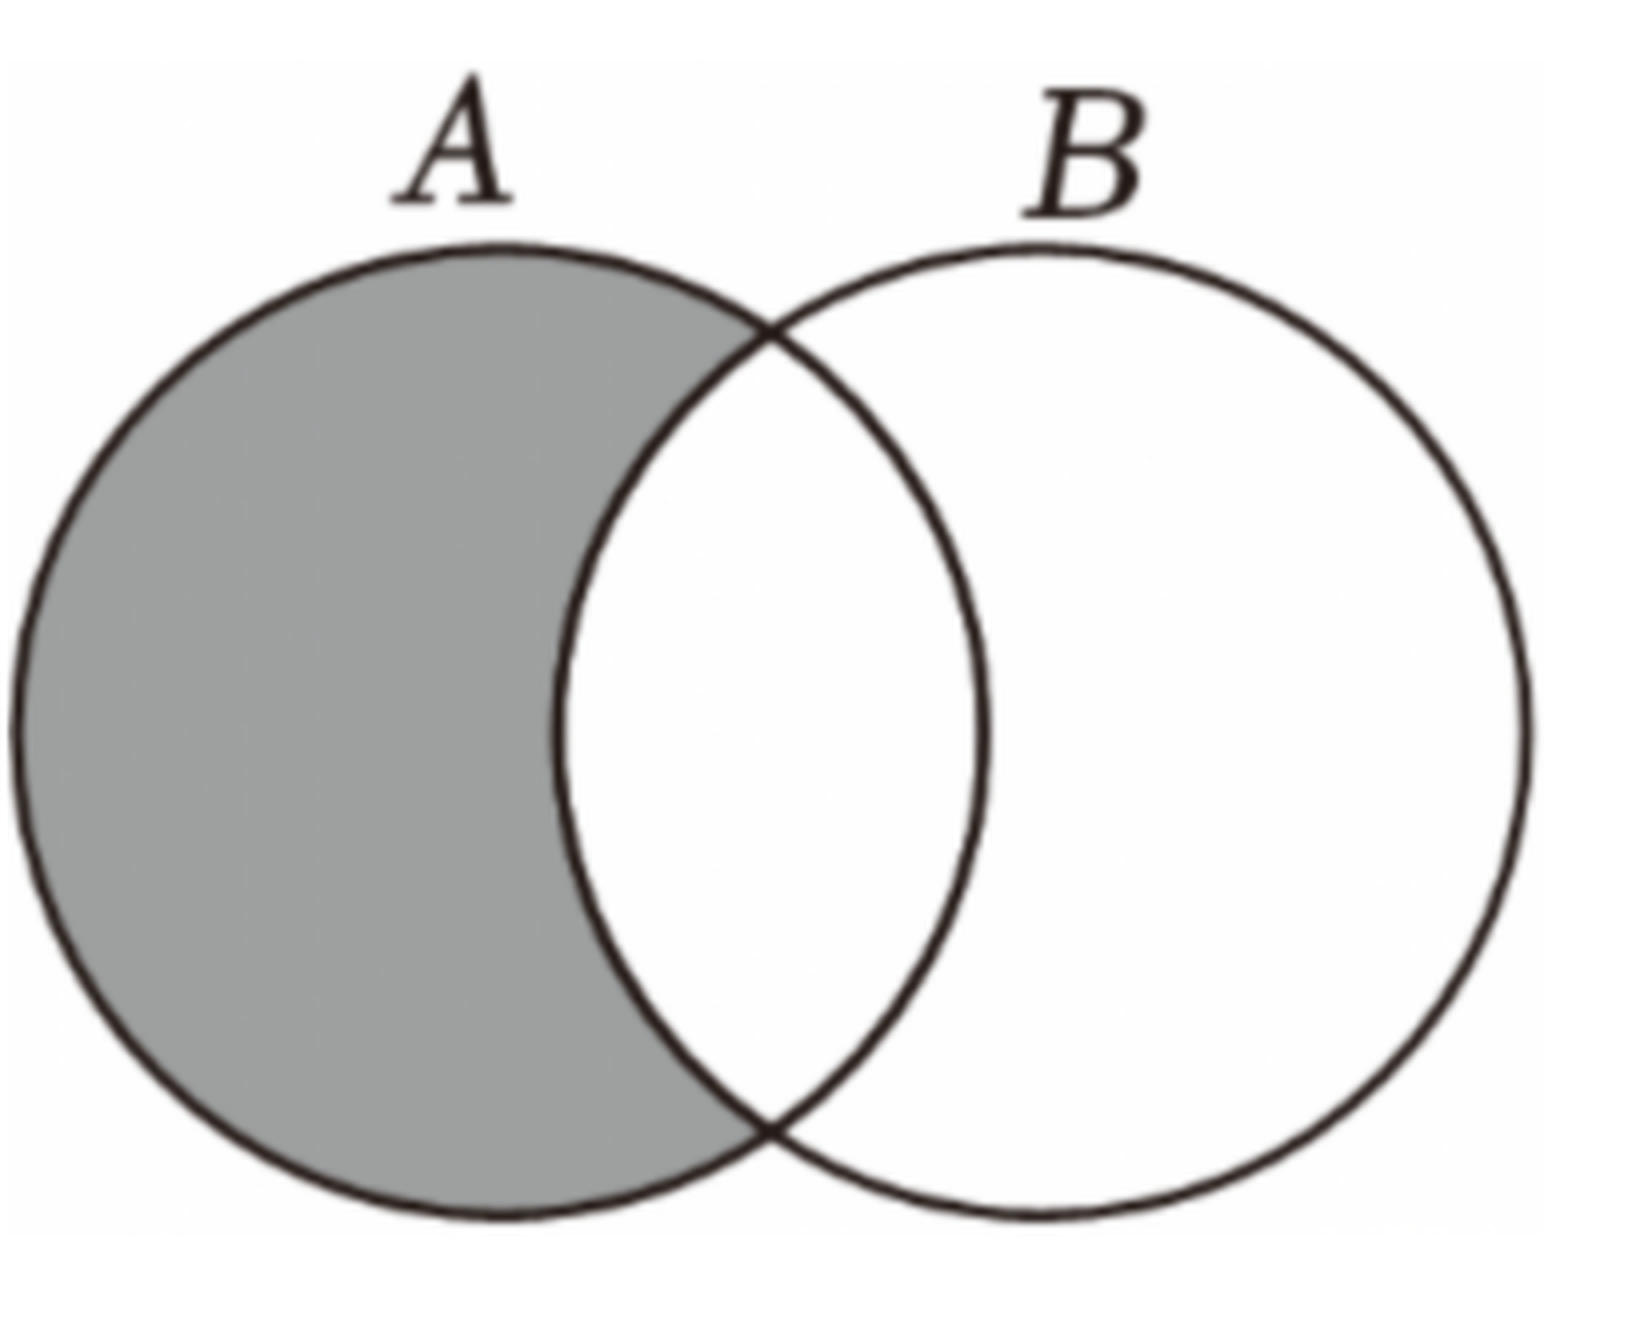
\includegraphics[width=0.30\textwidth]{figures/venn_A_minus_B_h38.png}
\end{center}

\ans{$\{1\}$}

\item 集合 $\{2,3,4,\cdots,2024,2025\}$ 的真子集的个数为 \blankline[4.4em].

\ans{$2^{2024}-1$}

\ifanswer
\solbegin
\step{集合 $\{2,3,4,\cdots,2024,2025\}$ 的真子集的个数为 $2^{2024}-1$.}
\solend

\fi

\item 已知集合 $A$ 中的元素都是正整数，其中最小的是 $1$，最大值是 $100$，除 $1$ 以外，每一个元
素都等于 $A$ 中的两个数（可以相同）的和，则集合 $A$ 中至少含有 \blankline[4.4em] 个元素.

\ans{$9$}

\ifanswer
\solbegin
\step{设 $A$ 中的数从小到大排列为 $1,a_1,a_2,\cdots,a_k,100$，}
\step{则 $a_1=1+1=2$；$3\leqslant a_2\leqslant 4$；$4\leqslant a_3\leqslant 8$；$5\leqslant a_4\leqslant 16$；$6\leqslant a_5\leqslant 32$；$7\leqslant a_6\leqslant 64$；}
\step{于是 $A$ 至少有八个数；}
\step{假设 $A$ 恰好有八个元素，由于 $a_5+a_6\leqslant 96<100$；}
\step{故必须有 $100=a_6+a_6$，$a_6=50$，}
\step{又 $a_4+a_5\leqslant 48$，同理 $a_5=25$，}
\step{但此时 $a_3+a_4\leqslant 24$，$a_5=2a_4$，$a_4=12.5$ 矛盾，}
\step{故 $A$ 不可能恰好有八个元素，因此 $A$ 至少有九个元素.}
\step{其九个数可以为 $1$，$2$，$3$，$6$，$12$，$13$，$25$，$50$，$100$.}
\solend

\fi

\item 已知集合 $\{x_1,x_2,x_3,x_4,x_5,x_6\}=\{1,2,3,4,5,6\}$，将 $x_i$ 与 $x_j$（其中 $i\in\{1,2,3\}$，
$j\in\{4,5,6\}$）的乘积 $x_ix_j$ 放入如图的 $3\times3$ 方格中，则方格中全部数之和的最大值为 \blankline[4.4em].

% 原卷的 $3\times3$ 方格是表格式内容（三行三列的公式），本稿按 高一03 的成例用 tabular 排出。
\begin{center}
\begin{tabular}{|c|c|c|}
\hline
$x_1x_4$ & $x_1x_5$ & $x_1x_6$ \\
\hline
$x_2x_4$ & $x_2x_5$ & $x_2x_6$ \\
\hline
$x_3x_4$ & $x_3x_5$ & $x_3x_6$ \\
\hline
\end{tabular}
\end{center}

\ans{$110$}

\ifanswer
\solbegin
\step{由表格数据得所有数之和为}
\step{$S=x_1x_4+x_1x_5+x_1x_6+x_2x_4+x_2x_5+x_2x_6+x_3x_4+x_3x_5+x_3x_6$，}
\step{所以 $S=(x_1+x_2+x_3)(x_4+x_5+x_6)$，}
\step{因为集合 $\{x_1,x_2,x_3,x_4,x_5,x_6\}=\{1,2,3,4,5,6\}$，}
\step{所以 $x_1+x_2+x_3+x_4+x_5+x_6=1+2+3+4+5+6=21$，}
\step{设 $t=x_1+x_2+x_3$，则 $6\leqslant t\leqslant 15$，$t\in\N^*$，}
\step{$S=t(21-t)=-\left(t-\dfrac{21}{2}\right)^2+\dfrac{441}{4}$，}
\step{当 $t=10$ 或 $t=11$ 时，$S=t(21-t)$ 取最大值，最大值为 $110$，}
\step{此时 $\{x_1,x_2,x_3\}=\{1,4,5\}$，$t=10$，所以可取最大值 $110$.}
\solend

\fi

\item 若 $[x]$ 表示不大于 $x$ 的最大整数，方程 $x^2-8[x]+7=0$ 的解集为 \blankline[4.4em].

\ans{$\{1,\sqrt{33},\sqrt{41},7\}$}

\ifanswer
\solbegin
\step{由题意，$x\geqslant[x]=\dfrac{x^2+7}{8}>0$，得 $x^2-8x+7\leqslant 0$，解得 $1\leqslant x\leqslant 7$，}
\step{$[x]=1$，$x^2=1$，$x=1$；}
\step{$[x]=2$，$x^2=9$，$x=3$ 与 $[x]=2$ 矛盾；}
\step{$[x]=3$，$x^2=17$，$x=\sqrt{17}$，$[x]=4$ 与 $[x]=3$ 矛盾；}
\step{$[x]=4$，$x^2=25$，$x=5$ 与 $[x]=4$ 矛盾；}
\step{$[x]=5$，$x^2=33$，$x=\sqrt{33}$，$[x]=5$；}
\step{$[x]=6$，$x^2=41$，$x=\sqrt{41}$，$[x]=6$；}
\step{$[x]=7$，$x^2=49$，$x=7$；}
\step{综上，方程 $x^2-8[x]+7=0$ 的解集为 $\{1,\sqrt{33},\sqrt{41},7\}$.}
\solend

\fi

\end{enumerate}

\bigsec{二、选择题}

\begin{enumerate}
\setcounter{enumi}{10}

\item 已知集合 $A=\{a,a^2\}$，$B=\{1,3\}$，若 $1\in A$，则 $A\cup B$ 中所有元素之和为\mbox{（\quad）}

\keepwithprev
A. $2$\qquad B. $3$\qquad C. $4$\qquad D. $5$

\ans{$B$}

\ifanswer
\solbegin
\step{因为 $1\in A$，集合 $A=\{a,a^2\}$，所以 $a=1$ 或 $a^2=1$，}
\step{若 $a=1$，则 $a=a^2$，与元素的互异性矛盾；}
\step{若 $a^2=1$，则 $a=1$（舍）或 $a=-1$，故 $A=\{-1,1\}$，$B=\{1,3\}$，}
\step{故 $A\cup B=\{-1,1,3\}$，所以 $A\cup B$ 中所有元素之和为 $-1+1+3=3$. 故选 $B$.}
\solend

\fi

\item 对于实数 $a$、$b$、$c$，下列命题正确的是\mbox{（\quad）}

\keepwithprev
A. 若 $a>b$，则 $ac^2>bc^2$\qquad B. 若 $a>b$，则 $a^2>b^2$

C. 若 $a>b$，则 $a|a|>b|b|$\qquad D. 若 $a>b>c>0$，则 $\dfrac{b}{a-b}<\dfrac{c}{a-c}$

\ans{$C$}

\ifanswer
\solbegin
\step{对于 $A$，若 $a>b$，$c=0$，则 $ac^2=bc^2$，故 $A$ 错误；}
\step{对于 $B$，若 $a>b$，取 $a=-1$，$b=-2$，则 $a^2<b^2$，故 $B$ 错误；}
\step{对于 $C$，若 $a>b>0$ 时，$a|a|-b|b|=a^2-b^2>0$，}
\step{当 $a>0>b$ 时，$a|a|-b|b|=a^2+b^2>0$，}
\step{当 $0>a>b$ 时，$a|a|-b|b|=b^2-a^2=(b-a)(b+a)>0$，}
\step{综上，若 $a>b$，则 $a|a|>b|b|$，故 $C$ 正确；}
\step{对于 $D$，若 $a>b>c>0$，$\dfrac{b}{a-b}-\dfrac{c}{a-c}=\dfrac{ab-bc-ac+bc}{(a-b)(a-c)}=\dfrac{a(b-c)}{(a-b)(a-c)}>0$，}
\step{故 $D$ 错误.}
\step{故选 $C$.}
\solend

\fi

\item 对于正整数集合 $A=\{a_1,a_2,\cdots,a_n\}(n\in\N^*,\ n\geqslant 3)$，如果去掉其中任意一个元素
$a_i(i=1,2,\cdots,n)$ 之后，剩余的所有元素组成的集合都能分为两个交集为空集的集合，且这
两个集合的所有元素之和相等，就称集合 $A$ 为平衡集. 记 $M=a_1+a_2+\cdots+a_n$. 若集合 $A$
是平衡集，并且存在 $a_i$ 为奇数，则集合 $A$ 中元素个数 $n$ 的奇偶性\mbox{（\quad）}

\keepwithprev
A. 与 $M$ 相关，既可以是奇数，又可以是偶数

B. 与 $M$ 无关，既可以是奇数，又可以是偶数

C. 与 $M$ 无关，必为偶数

D. 与 $M$ 无关，必为奇数

\ans{$D$}

\ifanswer
\solbegin
\step{正整数集合 $A=\{a_1,a_2,\cdots,a_n\}(n\in\N^*,\ n\geqslant 3)$，}
\step{因为集合 $A$ 是平衡集，设去掉元素 $a_i(i=1,2,\cdots,n)$，}
\step{由题意得 $A=A_1\cup A_2\cup\{a_i\}$，其中 $A_1\cap A_2=\varnothing$，}
\step{设集合 $A_1$ 和 $A_2$ 中的元素之和均为 $m$，所以 $M=2m+a_i$，其中 $i=1,2,\cdots,n$，}
\step{所以 $M-a_i=2m$，所以 $M-a_i$ 为偶数，其中 $i=1,2,\cdots,n$，}
\step{所以 $a_i(i=1,2,\cdots,n)$ 的奇偶性相同；}
\step{因为存在 $a_i$ 为奇数，所以 $a_i(i=1,2,\cdots,n)$ 均为奇数，}
\step{由 $M-a_i=2m$ 得 $M$ 也为奇数，且 $M=a_1+a_2+\cdots+a_n$，}
\step{所以 $n$ 也为奇数，所以 $n$ 必为奇数. 故选 $D$.}
\solend

\fi

\item 对于集合 $M=\{a\mid a=x^2-y^2,\ x\in\Z,\ y\in\Z\}$，给出如下三个结论：其中正确结论的个数
是\mbox{（\quad）}

\keepwithprev
①如果 $P=\{b\mid b=2n+1,\ n\in\Z\}$，那么 $P\sub M$；

②如果 $c=4n+2$，$n\in\Z$，那么 $c\notin M$；

③如果 $a_1\in M$，$a_2\in M$，那么 $a_1a_2\in M$.

\keepwithprev
A. $1$\qquad B. $2$\qquad C. $3$\qquad D. $0$

\ans{$C$}

\ifanswer
\solbegin
\step{对于①，$b=2n+1$，$n\in\Z$，则恒有 $2n+1=(n+1)^2-n^2$，}
\step{所以 $2n+1\in M$，即 $P=\{b\mid b=2n+1,n\in\Z\}$，则 $P\sub M$，①正确；}
\step{对于②，$c=4n+2$，$n\in\Z$，}
\step{若 $4n+2\in M$，则存在 $x$、$y\in\Z$ 使得 $x^2-y^2=4n+2$，}
\step{所以 $4n+2=(x+y)(x-y)$，又 $x+y$ 和 $x-y$ 同奇或同偶，}
\step{若 $x+y$ 和 $x-y$ 都是奇数，则 $(x+y)(x-y)$ 为奇数，而 $4n+2$ 是偶数；}
\step{若 $x+y$ 和 $x-y$ 都是偶数，则 $(x+y)(x-y)$ 能被 $4$ 整除，而 $4n+2$ 不能被 $4$ 整除，}
\step{所以 $4n+2\notin M$，即 $c\notin M$，②正确；}
\step{对于③，$a_1\in M$，$a_2\in M$，可设 $a_1=x_1^2-y_1^2$，$a_2=x_2^2-y_2^2$，$x_i$、$y_i\in\Z$；}
\step{则 $a_1a_2=(x_1^2-y_1^2)(x_2^2-y_2^2)=(x_1x_2)^2+(y_1y_2)^2-(x_1y_2)^2-(x_2y_1)^2$}
\step{$=(x_1x_2+y_1y_2)^2-(x_1y_2+x_2y_1)^2\in M$，那么 $a_1a_2\in M$，③正确.}
\step{综上，正确的命题是①②③. 故选 $C$.}
\solend

\fi

\end{enumerate}

\bigsec{三、解答题}

\begin{enumerate}
\setcounter{enumi}{14}

\item 已知 $A=\{x\mid a\leqslant x\leqslant -a+3\}$，$B=\{x\mid x<-1\text{ 或 }x>5\}$.

\begin{enumerate}[label=(\arabic*)]

\item 若 $A\cap B=\varnothing$，求 $a$ 的取值范围；

\item 若 $A\cup B=\R$，求 $a$ 的取值范围.

\end{enumerate}

\ans{（1）$[-1,+\infty)$；（2）$(-\infty,-2]$}

\ifanswer
\solbegin
\stepm{(1)}{①当 $A=\varnothing$ 时，$A\cap B=\varnothing$，需满足 $a>-a+3$，解得 $a>\dfrac32$，}
\step{故 $a$ 的取值范围为 $\left(\dfrac32,+\infty\right)$.}
\step{②当 $A\neq\varnothing$ 时，要使 $A\cap B=\varnothing$，需满足
$\begin{cases}a\leqslant\dfrac32\\[4pt] -a+3\leqslant 5\\[4pt] a\geqslant -1\end{cases}$，解得 $-1\leqslant a\leqslant\dfrac32$.}
\step{综上所述，$a$ 的取值范围是 $[-1,+\infty)$.}
\stepm{(2)}{因为 $A\cup B=\R$，$A=\{x\mid a\leqslant x\leqslant -a+3\}$，$B=\{x\mid x<-1\text{ 或 }x>5\}$，}
\step{所以 $\begin{cases}-a+3\geqslant 5\\[4pt] a\leqslant -1\end{cases}$，解得 $a\leqslant -2$，故所求 $a$ 的取值范围为 $(-\infty,-2]$.}
\solend

\fi

\ansspace[6]

\item 已知集合 $A=\{x\mid mx^2+x-2=0\}$，$B=\{x\mid 2x^2-5x-12=0\}$.

\begin{enumerate}[label=(\arabic*)]

\item 若 $A$ 中有且仅有 $1$ 个元素，求实数 $m$ 的值；

\item 已知集合 $C=A\cup B$，若 $C$ 的真子集有且仅有 $3$ 个，求实数 $m$ 的取值范围.

\end{enumerate}

\ans{（1）$m=0$ 或 $m=-\dfrac18$；（2）$\left\{m\mid m\leqslant -\dfrac18\right\}$}

\ifanswer
\solbegin
\stepm{(1)}{若 $m=0$，方程化为 $x-2=0$，此时方程有且仅有一个根 $x=2$；}
\step{若 $m\neq 0$，则 $\Delta=1^2-4\times m\times(-2)=0$，即 $m=-\dfrac18$ 时，}
\step{方程有两个相等的实根，此时集合 $A$ 中有且仅有一个元素，}
\step{所以实数 $m$ 的值为 $m=0$ 或 $m=-\dfrac18$；}
\stepm{(2)}{$B=\{x\mid 2x^2-5x-12=0\}=\left\{-\dfrac32,4\right\}$，}
\step{因为 $C=A\cup B$，若 $C$ 的真子集有且仅有 $3$ 个，则 $C$ 中有两个元素，}
\step{所以 $A\sub B$，由（1）得 $m=0$ 时，$A=\{2\}$，不符合 $A\sub B$，}
\step{当 $m\neq 0$ 时，若 $\Delta=1^2-4\times m\times(-2)<0$，解得 $m<-\dfrac18$，}
\step{此时 $A=\varnothing$，符合 $A\sub B$，}
\step{若 $\Delta=1^2-4\times m\times(-2)=0$，解得 $m=-\dfrac18$，}
\step{此时方程 $mx^2+x-2=0$ 的根为 $x=4$，集合 $A=\{4\}$，符合 $A\sub B$，}
\step{若 $\Delta=1^2-4\times m\times(-2)>0$，由 $A\sub B$，得 $A=\left\{-\dfrac32,4\right\}$，}
\step{此时有 $-\dfrac32+4=-\dfrac1m$ 且 $-\dfrac32\times 4=-\dfrac2m$，无解，}
\step{综上所述，实数 $m$ 的取值范围为 $\left\{m\mid m\leqslant -\dfrac18\right\}$.}
\solend

\fi

\ansspace[6]

\item 设 $A$ 是非空实数集，且 $0\notin A$. 若对于任意的 $x$、$y\in A$，都有 $xy\in A$，则称集合 $A$ 具
有性质 $P_1$；若对于任意的 $x$、$y\in A$，都有 $\dfrac xy\in A$，则称集合 $A$ 具有性质 $P_2$.

\begin{enumerate}[label=(\arabic*)]

\item 写出一个恰含有两个元素且具有性质 $P_1$ 的集合 $A$，并说明理由；

\item 证明：“非空实数集 $A$ 具有性质 $P_1$”是“非空实数集 $A$ 具有性质 $P_2$”的必要非充分条
件.

\end{enumerate}

\ans{（1）$A=\{-1,1\}$，理由见解析；（2）见解析}

\ifanswer
\solbegin
% 注：原卷本题 (1) 的解析里“证明”一词重复出现两次（一次接在分号后、一次另起一行），
%     本稿照原卷重复录入，未去重。
\stepm{(1)}{$A=\{-1,1\}$，证明：恰含有两个元素且具有性质 $P_1$ 的集合 $A=\{-1,1\}$；}
\step{证明：$1\times 1=1\in A$，$1\times(-1)=-1\in A$，$-1\times 1=-1\in A$，$-1\times(-1)=1\in A$；}
\stepm{(2)}{若集合 $A$ 具有性质 $P_2$，不妨设 $a\in A$，}
\step{由非空数集 $A$ 具有性质 $P_2$，有 $\dfrac aa=1\in A$.}
\step{①$A=\{1\}$，易得此时集合 $A$ 具有性质 $P_1$.}
\step{②数集 $A$ 只含有两个元素，不妨设 $A=\{1,a_1\}$，}
\step{由 $\dfrac{1}{a_1}=a_1$，且 $a_1\neq 1$，解得 $a_1=-1$，此时集合 $A$ 具有性质 $P_1$.}
\step{③实数集 $A$ 含有两个以上的元素，不妨设不为 $1$ 的元素 $a_1$、$a_2\in A$，}
\step{则有 $\dfrac{1}{a_1}\in A$，由于集合 $A$ 具有性质 $P_2$，}
\step{所以有 $a_2\div\dfrac{1}{a_1}=a_1a_2\in A$，这说明集合 $A$ 具有性质 $P_1$.}
\step{综上，若非空实数集 $A$ 具有性质 $P_2$，则集合 $A$ 具有性质 $P_1$，}
\step{所以“非空实数集 $A$ 具有性质 $P_1$”是“非空实数集 $A$ 具有性质 $P_2$”的}
\step{必要条件.}
\step{取正偶数集 $A=\{x\mid x=2n,\ n\in\N^*\}$，}
\step{对任意的 $2m$、$2n\in A$，$m$、$n\in\N^*$，}
\step{有 $2m\times 2n=4mn\in A$，故 $A$ 具有性质 $P_1$，}
\step{取 $x=2$，$y=4$，则 $\dfrac xy=\dfrac12\notin A$，故 $A$ 不具有性质 $P_2$，}
\step{所以“非空实数集 $A$ 具有性质 $P_1$”不是“非空实数集 $A$ 具有性质 $P_2$”的}
\step{充分条件.}
\step{综上，“非空实数集 $A$ 具有性质 $P_1$”是“非空实数集 $A$ 具有性质 $P_2$”的}
\step{必要非充分条件.}
\solend

\fi

\ansspace[8]

\item 已知命题 $p$：关于 $x$ 的方程 $x^2+mx+1=0$ 有两个不同的正根；命题 $q$：关于 $x$ 的方程
$4x^2+4(m-2)x=-1$ 有实根.

\begin{enumerate}[label=(\arabic*)]

\item 若命题 $q$ 为假命题，求整数 $m$ 的解集；

\item 若命题 $p$ 为真命题，且关于 $x$ 的方程 $x^2+mx+1=0$ 的两个实数根 $x_1$、$x_2$ 满足
$3x_1+2x_2=5$，求实数 $m$ 的取值集合；

\item 若命题 $p$ 和命题 $q$ 有且仅有一个成立，求实数 $m$ 的取值范围.

\end{enumerate}

\ans{（1）$\{2\}$；（2）$\left\{-\dfrac{13}{6}\right\}$；（3）$[-2,1]\cup[3,+\infty)$}

\ifanswer
\solbegin
\stepm{(1)}{命题 $q$：关于 $x$ 的方程 $4x^2+4(m-2)x=-1$ 有实根为假命题，}
\step{即 $4x^2+4(m-2)x+1=0$ 无实根，}
\step{则 $\Delta=16(m-2)^2-16<0$，则 $1<m<3$，则整数 $m$ 的解集为 $\{2\}$；}
\stepm{(2)}{若命题 $p$ 为真命题，且关于 $x$ 的方程 $x^2+mx+1=0$ 的两个实数根 $x_1$、$x_2$，}
\step{满足 $3x_1+2x_2=5$，则方程 $x^2+mx+1=0$ 有两个不同的正根，}
\step{则 $\begin{cases}\Delta=m^2-4>0\\[4pt] x_1+x_2=-m>0\end{cases}$，则 $m<-2$，}
\step{又 $\begin{cases}x_1+x_2=-m\\[4pt] x_1x_2=1\\[4pt] 3x_1+2x_2=5\end{cases}$，
则 $\begin{cases}x_1=5+2m\\[4pt] x_2=-3m-5\end{cases}$，则 $(5+2m)(-3m-5)=1$，}
\step{得 $m=-2$ 或 $m=-\dfrac{13}{6}$，又因为 $m<-2$，所以 $m=-\dfrac{13}{6}$，}
\step{所以实数 $m$ 的取值集合为 $\left\{-\dfrac{13}{6}\right\}$；}
\stepm{(3)}{由（2）得当 $p$ 为真时，则有 $m<-2$，}
\step{当 $q$ 为真时，$\Delta=16(m-2)^2-16\geqslant 0$，解得 $m\leqslant 1$ 或 $m\geqslant 3$，}
\step{又因为命题 $p$ 和命题 $q$ 只有一个为真，所以
$\begin{cases}m<-2\\[4pt] 1<m<3\end{cases}$ 或 $\begin{cases}m\geqslant -2\\[4pt] m\leqslant 1\text{ 或 }m\geqslant 3\end{cases}$，}
\step{解得 $-2\leqslant m\leqslant 1$ 或 $m\geqslant 3$，所以实数 $m$ 的取值范围为 $[-2,1]\cup[3,+\infty)$.}
\solend

\fi

\ansspace[8]

% 注：原卷此处作“设 $n\in\N^*$，集合含有 $3n$ 个元素”，**漏了符号 $U$**（应作“集合 $U$
%     含有 $3n$ 个元素”）——$U$ 直到本句末尾“则称 $U$ 为三分集合”才出现、此前无定义。
%     本稿照录未补，见文件头“原卷笔误/存疑”⑦。
\item 设 $n\in\N^*$，集合含有 $3n$ 个元素，若存在三个 $n$ 元集合 $A$、$B$、$C$ 满足如下两个条件，
则称 $U$ 为三分集合.

①$U=A\cup B\cup C$；

②$A$、$B$、$C$ 元素可分别排列为有序数组 $(a_1,a_2,\cdots,a_n)$，$(b_1,b_2,\cdots,b_n)$ 及
$(c_1,c_2,\cdots,c_n)$，使得对 $\forall i=1,2,\cdots,n$，均有 $a_i+b_i=c_i$.

特别地，当 $U=\{1,2,3,4,\cdots,3n-2,3n-1,3n\}$ 为三分集合时，称 $n$ 为完美三分数.

如：因为 $U=\{1,2,3\}$ 为三分集合，所以 $n=1$ 为最小完美三分数.

\begin{enumerate}[label=(\arabic*)]

\item 请判断下列两个集合是否为三分集合（直接写出结论）：

$U_1=\{1,2,3,4,5,6\}$，$U_2=\{1,3,5,7,8,9,10,11,12\}$；

\item 求出大于 $1$ 的最小完美三分数；

\item 请判断是否存在无穷多个完美三分数？若存在，请说明理由；若不存在，则求出最大的
完美三分数.

\end{enumerate}

\ans{（1）$U_1$ 不是三分集合，$U_2$ 是三分集合；（2）$4$；（3）存在，理由见解析}

\ifanswer
\solbegin
\stepm{(1)}{(i)$U_1=\{1,2,3,4,5,6\}$ 不是三分集合，下面用反证法证明：}
\step{证明：假设 $U=\{1,2,3,4,5,6\}$ 是三分集合，}
\step{设 $A=\{a_1,a_2\}$，$B=\{b_1,b_2\}$，$C=\{c_1,c_2\}$，不妨设 $c_1<c_2$，}
\step{因为 $a_1+b_1=c_1$，$a_2+b_2=c_2$，}
\step{所以 $a_1+b_1+a_2+b_2+c_1+c_2=2(c_1+c_2)=1+2+3+4+5+6=21$，}
% 注：原卷此步印“所以 $c_1+c_2=2$”，与上一行的 $2(c_1+c_2)=21$ **不自洽**
%     （应作 $\dfrac{21}2$）；同题 $n=3$ 处的同型推理原卷写的是 $\dfrac{45}2$，故此处是原卷笔误。
%     本稿照录未改，见文件头“原卷笔误/存疑”⑧。
\step{所以 $c_1+c_2=2$，这与 $c_1,c_2\in\N^*$ 矛盾，故假设错误，}
\step{故 $U_1=\{1,2,3,4,5,6\}$ 不是三分集合；}
\step{(ii)$U_2=\{1,3,5,7,8,9,10,11,12\}$ 是三分集合，理由如下：}
\step{令 $A=\{1,3,5\}$，$B=\{9,8,7\}$，$C=\{10,11,12\}$，}
\step{则 $A\cup B\cup C=U=\{1,3,5,7,8,9,10,11,12\}$，满足条件①；}
\step{又 $1+9=10$；$3+8=11$；$5+7=12$，所以满足条件②，}
\step{所以 $U_2=\{1,3,5,7,8,9,10,11,12\}$ 是三分集合；}
\stepm{(2)}{由（1）得，当 $n=2$ 时，$U=\{1,2,3,4,5,6\}$ 不是三分集合；}
\step{当 $n=3$ 时，$U=\{1,2,3,4,5,6,7,8,9\}$，}
\step{假设 $U=\{1,2,3,4,5,6,7,8,9\}$ 是三分集合，}
\step{同理由 $a_1+b_1+a_2+b_2+a_3+b_3+c_1+c_2+c_3$}
\step{$=2(c_1+c_2+c_3)=1+2+\cdots+9=45$，$c_1+c_2+c_3=\dfrac{45}{2}$，}
\step{可推出与 $c_1$、$c_2$、$c_3\in\N^*$ 矛盾，故假设也错误，}
\step{所以 $U=\{1,2,3,4,5,6,7,8,9\}$ 不是三分集合；}
\step{当 $n=4$ 时，$U=\{1,2,3,\cdots,12\}$，}
\step{存在三个 $4$ 元集合 $A=\{1,2,4,3\}$，$B=\{5,8,7,9\}$，$C=\{6,10,11,12\}$，}
\step{满足 $U=\{1,2,3,\cdots,12\}$ 为三分集合的两个条件，}
\step{故大于 $1$ 的最小完美三分数为 $4$；}
\stepm{(3)}{存在无穷多个完美三分数，理由如下：}
\step{由题意得，$n=1$ 为最小完美三分数，}
\step{当 $n=5$ 时，$U=\{1,2,3,\cdots,15\}$，}
\step{存在三个 $5$ 元集合 $A=\{1,3,5,7,2\}$，$B=\{11,10,9,8,4\}$，$C=\{12,13,14,15,6\}$，}
\step{满足三分集合的条件，故 $5$ 为完美三分数；}
\step{当 $n=21$ 时，$U=\{1,2,3,\cdots,63\}$，}
\step{存在如下三个 $21$ 元的集合满足三分集合的条件：}
\step{$A=\{1,3,5,7,\cdots,29,31,2,6,10,14,4\}$，}
\step{$B=\{47,46,45,44,\cdots,33,32,22,20,18,16,8\}$，}
\step{$C=\{48,49,50,51,\cdots,62,63,24,26,28,30,12\}$，}
\step{故 $21$ 为完美三分数.}
\step{首先证明：若 $n=k$，$k\in\N^*$ 为三分完美数，}
\step{则 $n=4k+1$，$k\in\N^*$ 也为三分完美数，}
% 注：下一行原卷印作“$U_{k+1}=U_{k+1}=\{2,3,\cdots,12k+3\}$”——等号两边记号相同，
%     依上下文疑当作 $U'_{k+1}=U_{4k+1}$，且此处集合自 2 起（前文 $U_{4k+1}$ 自 1 起）；
%     本稿照录原卷，未代为改写。
\step{证明：记 $U_k=\{1,2,3,\cdots,3k\}$，$U_{4k+1}=\{1,2,3,\cdots,12k+3\}$，}
\step{若 $n=k$，$k\in\N^*$ 为三分完美数，则 $U_k$ 为三分集合，}
\step{即存在三个 $k$ 元集合 $A$、$B$、$C$ 满足如下两个条件，}
\step{①$U_k=A\cup B\cup C$；}
\step{②$A$、$B$、$C$ 元素可分别排列为有序数组 $(a_1,a_2,\cdots,a_k)$，}
\step{$(b_1,b_2,\cdots,b_k)$ 及 $(c_1,c_2,\cdots,c_k)$，}
\step{使得对 $\forall i=1,2,3,\cdots,k$，均有 $a_i+b_i=c_i$，}
\step{则可得到对 $\forall i=1,2,3,\cdots,k$，$2a_i+2b_i=2c_i$，}
\step{故集合 $\{2,4,6,\cdots,6k\}$ 也满足三分集合的两个条件，其也为三分集合，}
\step{下面记集合 $\{2,4,6,\cdots,6k\}=2U_k$，}
\step{对 $n=4k+1$，集合 $U_{k+1}=U_{k+1}=\{2,3,\cdots,12k+3\}=(2U_k)\cup\complement_{U_{4k+1}}(2U_k)$，}
\step{构造集合 $A'=\{1,3,5,7,\cdots,6k+1\}$，共有 $3k+1$ 个奇数；}
% 注：下一行原卷印作“$B'=\{6k+3k+2,6k+3k+1,6k+3k,6k+3k-1,\cdots,6k+2\}$”，
%     按与后文 $C'$ 相接，前四项当写作 $9k+2$、$9k+1$、$9k$、$9k-1$；本稿照录原卷。
\step{集合 $B'=\{6k+3k+2,6k+3k+1,6k+3k,6k+3k-1,\cdots,6k+2\}$，}
\step{共有 $3k+1$ 个逐个减小的连续正整数；}
\step{集合 $C'=\{9k+3,9k+4,9k+5,9k+6,\cdots,12k+3\}$，}
\step{共有 $3k+1$ 个逐个增大的连续正整数；}
\step{得这三个 $3k+1$ 元集合 $A'$、$B'$、$C'$ 满足如下两个条件，}
\step{①集合 $A'\cup B'\cup C'=\complement_{U_{4k+1}}(2U_k)$；}
\step{②$A'$、$B'$、$C'$ 元素可分别排列为有序数组 $(a_1,a_2,\cdots,a_{3k+1})$，}
\step{$(b_1,b_2,\cdots,b_{3k+1})$ 及 $(c_1,c_2,\cdots,c_{3k+1})$，}
\step{使得对 $\forall i=1,2,3,\cdots,3k+1$，均有 $a_i+b_i=c_i$；}
\step{故 $\complement_{U_{4k+1}}(2U_k)$ 为三分集合，而已知 $U_k$ 为三分集合，}
\step{将其对应与 $A'$、$B'$、$C'$ 合并，}
% 注：原卷此处印“令 $A''=A\cup A'$”（$B''$、$C''$ 同）。按同段上文“记集合
%     $\{2,4,6,\cdots,6k\}=2U_k$”，此处疑当作 $A''=2A\cup A'$——否则
%     $A''\cup B''\cup C''=U_k\cup\complement_{U_{4k+1}}(2U_k)\neq U_{4k+1}$，与本段结论冲突。
%     本稿照录未改，见文件头“原卷笔误/存疑”⑨。
\step{令 $A''=A\cup A'$，$B''=B\cup B'$，$C''=C\cup C'$，}
\step{则这三个 $4k+1$ 元集合 $A''$、$B''$、$C''$，}
\step{满足 $A''\cup B''\cup C''=U_{4k+1}$，且满足条件②，}
\step{故 $U_{4k+1}=\{1,2,3,\cdots,12k+3\}$ 为三分集合，}
\step{因此可得，若 $n=k$ 为三分完美数，则 $n=4k+1$ 也为三分完美数，}
\step{由 $1$，$5$，$21$ 为完美三分数，结合所证结论得，存在无穷多个完美三分数.}
\solend

\fi

\ansspace*[12]

\end{enumerate}

\end{document}
"
%
% 原始材料是微信公众号图文（公众号“魔都数学加油站”连载“27学年高一 38”，署名“破晓”，
% 2026-09-26 21:29 发布，原文标题“27学年高一38——2026-2027年上海市大同中学高一上周末作业3”，
% 原文链接 https://mp.weixin.qq.com/s/O_O60vCIiGi2xponAo4irw ），正文为 12 张 PNG 页。
% **同一篇里各页分辨率不一致**（2560×3620 与 4762×6735 两档混排：第 1、10、11、12 页为
% 2560×3620，第 2—9 页为 4762×6735）。原文本身就是一份**讲评版**——有的题下方只印
% 【答案】行，有的只印【解析】。试题文字、答案与解析均照原卷录入，未改内容。卷面的粉色
% 斜水印“魔都数学加油站”属水印，未录入。
%
% 本卷共 **17 题**：填空题 8 题（第 3—10 题）、选择题 4 题（第 11—14 题）、解答题 5 题
% （第 15—19 题）；插图 1 张（第 6 题 Venn 图）。三版页数：试卷版 4 页 / 答案版 11 页 /
% 紧凑版 3 页，`Overfull`／`Underfull`／`Missing character` 告警均为 0。
%
% 卷首标题：原卷印作“2026-2027 年大同中学高一上周末作业 3”（公众号原文标题里的“上海市”
% 三字卷面标题行没有，本稿照卷面），年份区间按全稿惯例排 en dash，前缀照原卷保留“年”。
%
% 与原卷的排版差异（均已在 README“说明”中交代）：
%   ① 原文自**第 3 题**起（第 1、2 题未在该文中发布），故本稿题号亦自 3 起，填空题以
%      \setcounter{enumi}{2} 起编；选择、解答两节各按上一节末号另设 \setcounter
%      （选择题 \setcounter{enumi}{10}、解答题 \setcounter{enumi}{14}）；
%   ② 原卷本就印有“一、填空题”“二、选择题”“三、解答题”三节标题，本稿照原卷分节，
%      只把标题改排成全稿统一的“大节标题”样式；
%   ③ 原卷是“讲评版”：第 3、6 题只印【答案】行，第 4、5、7、8、9、10 题与第 11—19 题印
%      【解析】；本稿统一改为试卷版隐去、答案版以 \ans{}／\ifanswer 块给出，两版彻底分离。
%      其中第 4、5、7、8、9、10 题与第 11—14 题的答案，原卷写在【解析】末句，本稿另提为
%      \ans{}；第 15—19 题原卷只有【解析】、无独立答案行，本稿亦补了摘要式 \ans{}。
%      **故本卷 17 题每题都有 \ans**——比“只印【解析】的填空、解答题不另提 \ans”的
%      高一31／高一34 更彻底，与 高一21 第 11 题（填空，答案在【解析】末句，本稿另提）同类；
%      （本仓对“另提 \ans{}”的做法各卷不一，见 README 对应专记的核对面。）
%   ④ 数集记号原卷两套并用：第 3、5 题的实数集作粗体 $\mathbf{R}$，第 8、14、17、18 题等的
%      整数集、自然数集作斜体 $Z$、$N$，本稿按全稿惯例统一写作 $\R$、$\Z$、$\N$；
%   ⑤ 原卷填空的横线宽度不一（约 1.8—3.6 字宽），本稿按全稿惯例统一排 \blankline[4.4em]；
%   ⑥ 中文括注原卷用半角“(  )”，本稿按全稿惯例排全角；选择题的作答括注统一排
%      \mbox{（\quad）}（第 14 题的作答括注原卷印在 ①②③ 三个命题**之前**，本稿照原卷次序）；
%      数学式内部的括注（如第 4 题的 $p\%(0<p<100)$、第 13 题的 $a_i(i=1,2,\cdots,n)$）照原样
%      留在行内公式里，未改全角；
%   ⑦ 原卷并列的字母（“x,y”“a,b,c”）不加标点或作半角逗号，本稿按全稿惯例改排顿号；
%   ⑧ 第 6 题的 Venn 图取原卷截图、4× LANCZOS 放大（figures/venn_A_minus_B_h38.png，
%      见该处 \includegraphics 前的注释）；第 9 题的 $3\times3$ 方格属**表格式**内容，
%      本稿按 高一03 的成例用 tabular 排出，未截图；
%   ⑨ 原卷未印副标题，本稿按**本卷实际内容**补出副标题“集合与常用逻辑用语”（依据见下条）；
%   ⑩ 原卷【解析】**一个印刷行照录为一条 `\step`**（原卷的折行也照录为独立一条，如第 17 题
%      末三处“…的”／“必要条件.”这类跨行句、第 9 题“由表格数据得所有数之和为”／
%      “$S=\cdots$，”），使答案版的排布与原卷讲评版逐行对应；全卷 15 处【解析】合计
%      **191 条 `\step` ＝ 原卷 191 行**（逐处：5、5、1、9、9、9、4、9、9、12、6、14、21、13、65）。
%
% 副标题（\examtitlest 第二个参数）：本卷卷面未印副标题，由本稿补出，取值按 2026-09-26 起的
%   新口径“只用本卷实际内容的模块名”定为“集合与常用逻辑用语”。依据：全卷 17 题
%   （第 3—19 题）中，第 3、5、6、7、8、9、10、11、13、14、15、16、17、18、19 题共 15 题
%   是集合的运算与关系、子集计数、集合新定义（性质 $P_1$／$P_2$、平衡集、三分集合），以及
%   命题与逻辑（第 3 题即用反证法证明“$x+y>2\Rightarrow x>1$ 或 $y>1$”这一命题）；不等式只
%   出现在第 4 题（降价提价的应用比较）、第 12 题（不等式命题真假）与第 10 题解析里解一元
%   二次不等式，合计不足全卷的三分之一，故不并标“不等式”。
%
% 原卷笔误/存疑（均照抄原卷、未改，见源码中该处上方注释）：
%   ① 第 19 题 (3) 的证明里印作“集合 $U_{k+1}=U_{k+1}=\{2,3,\cdots,12k+3\}$”——等号两边
%      记号相同（依上下文疑当作 $U'_{k+1}=U_{4k+1}$），且此处集合自 $2$ 起，而前文
%      $U_{4k+1}=\{1,2,3,\cdots,12k+3\}$ 自 $1$ 起；本稿照录；
%   ② 第 19 题 (3) 的证明里印作
%      “$B'=\{6k+3k+2,6k+3k+1,6k+3k,6k+3k-1,\cdots,6k+2\}$”——按与后文
%      $C'=\{9k+3,9k+4,9k+5,9k+6,\cdots,12k+3\}$ 相接，前四项当写作 $9k+2$、$9k+1$、
%      $9k$、$9k-1$（即 $6k+3k+2$ 等），原卷即作“$6k+3k+\cdots$”形式，本稿照录；
%   ③ 第 19 题的术语前后不一：题干与 (1)(2)(3) 用“完美三分数”，而 (3) 的证明里五次写作
%      “三分完美数”（词序不同）；本稿五处都照录；
%   ④ 第 14 题题干作“给出如下三个结论：其中正确结论的个数是（\quad）”，此处冒号疑当作
%      逗号，本稿照录；
%   ⑤ 第 17 题题干作“非空实数集”，其解析有一处写作“非空数集”；本稿照录；
%   ⑥ 第 17 题 (1) 的【解析】原卷连写“…集合 $A=\{-1,1\}$；证明：…；证明：…”，“证明”
%      一词重复出现两次（第一次在分行处、第二次另起一行），本稿照原卷重复录入，未去重。
%   ⑦ 第 19 题**题干漏字**：原卷作“19.设 $n\in\N^*$，集合含有 $3n$ 个元素…则称 $U$ 为
%      三分集合”——首句漏了符号 $U$（应作“集合 $U$ 含有 $3n$ 个元素”），$U$ 直到结论句
%      才出现、此前无定义；本稿照录未补（见该处上方注释）。
%   ⑧ 第 19(1)(i) 的【解析】**自相矛盾**：上一行印“$a_1+b_1+a_2+b_2+c_1+c_2=2(c_1+c_2)
%      =1+2+3+4+5+6=21$”，下一行却印“所以 $c_1+c_2=2$”（由 $2(c_1+c_2)=21$ 应得
%      $c_1+c_2=\dfrac{21}2$，非整数、才与 $c_1,c_2\in\N^*$ 矛盾）；同题 $n=3$ 处的同型
%      推理原卷就写对了（$\dfrac{45}2$），故此处是原卷笔误；本稿照录未改（见该处上方注释）。
%   ⑨ 第 19(3) 的【解析】印“令 $A''=A\cup A'$，$B''=B\cup B'$，$C''=C\cup C'$”——按同段
%      上文“记集合 $\{2,4,6,\cdots,6k\}=2U_k$”，$A''$ 等疑当作 $2A\cup A'$（$B''$、$C''$ 同），
%      否则 $A''\cup B''\cup C''=U_k\cup\complement_{U_{4k+1}}(2U_k)\neq U_{4k+1}$；本稿照录未改
%      （见该处上方注释）。

\documentclass[a4paper,11pt]{article}
\usepackage{common}

\begin{document}

\examtitlest[3]{2026--2027 年大同中学高一上周末作业 3}{集合与常用逻辑用语}

\bigsec{一、填空题}

\begin{enumerate}
% 原卷填空题自第 3 题起（第 1、2 题未在该文中发布），须与选择、解答两节的 \setcounter 对齐
\setcounter{enumi}{2}

\item 设 $x$、$y\in\R$，若 $x+y>2$，则 $x>1$ 或 $y>1$ 是真命题. 这个命题可以用反证法去证明，
可以假设：\blankline[4.4em].

\ans{$x\leqslant 1$ 且 $y\leqslant 1$}

\item 已知某商品的原价为 $a$ 元，由于市场原因，先降价 $p\%(0<p<100)$ 出售，一段时间后，
再提价 $p\%$ 出售，则该商品提价后的售价 \blankline[4.4em] 该商品的原价（填“高于”“低于”或“等于”）.

\ans{低于}

\ifanswer
\solbegin
\step{由题意得第一次降价后的售价为 $a(1-p\%)$ 元，}
\step{第二次提价后的售价为 $a(1-p\%)(1+p\%)$ 元，}
\step{因为 $0<p<100$，所以 $0<p\%<1$，}
\step{因为 $a(1-p\%)(1+p\%)=a[1-(p\%)^2]<a$，}
\step{即该商品提价后的售价低于该商品的原价.}
\solend

\fi

\item 若集合 $A=\{x\mid ax^2+ax+1=0,\ a\in\R,\ x\in\R\}$ 的子集只有两个，则实数 $a=$ \blankline[4.4em].

\ans{$4$}

\ifanswer
\solbegin
\step{集合 $A=\{x\mid ax^2+ax+1=0\}$ 的子集只有两个，}
\step{所以 $A$ 有且只有一个元素，}
\step{①若 $a=0$，则 $A=\varnothing$ 不成立；}
\step{②若 $a\neq 0$，则 $\Delta=a^2-4a=0$，解得 $a=4$（$0$ 舍）.}
\step{故 $a=4$.}
\solend

\fi

\item 如图，已知集合 $A=\{1,2,3,4,5\}$，集合 $B=\{2,3,4,5,9\}$，则图中阴影部分所表示的
集合为 \blankline[4.4em].

% 图取原卷截图（01.png，2560×3620）右栏，4× LANCZOS 放大；为避免与 高一11 的
% figures/venn_A_minus_B.png 同名，按 高一32 的成例加 _h38 后缀。
\begin{center}
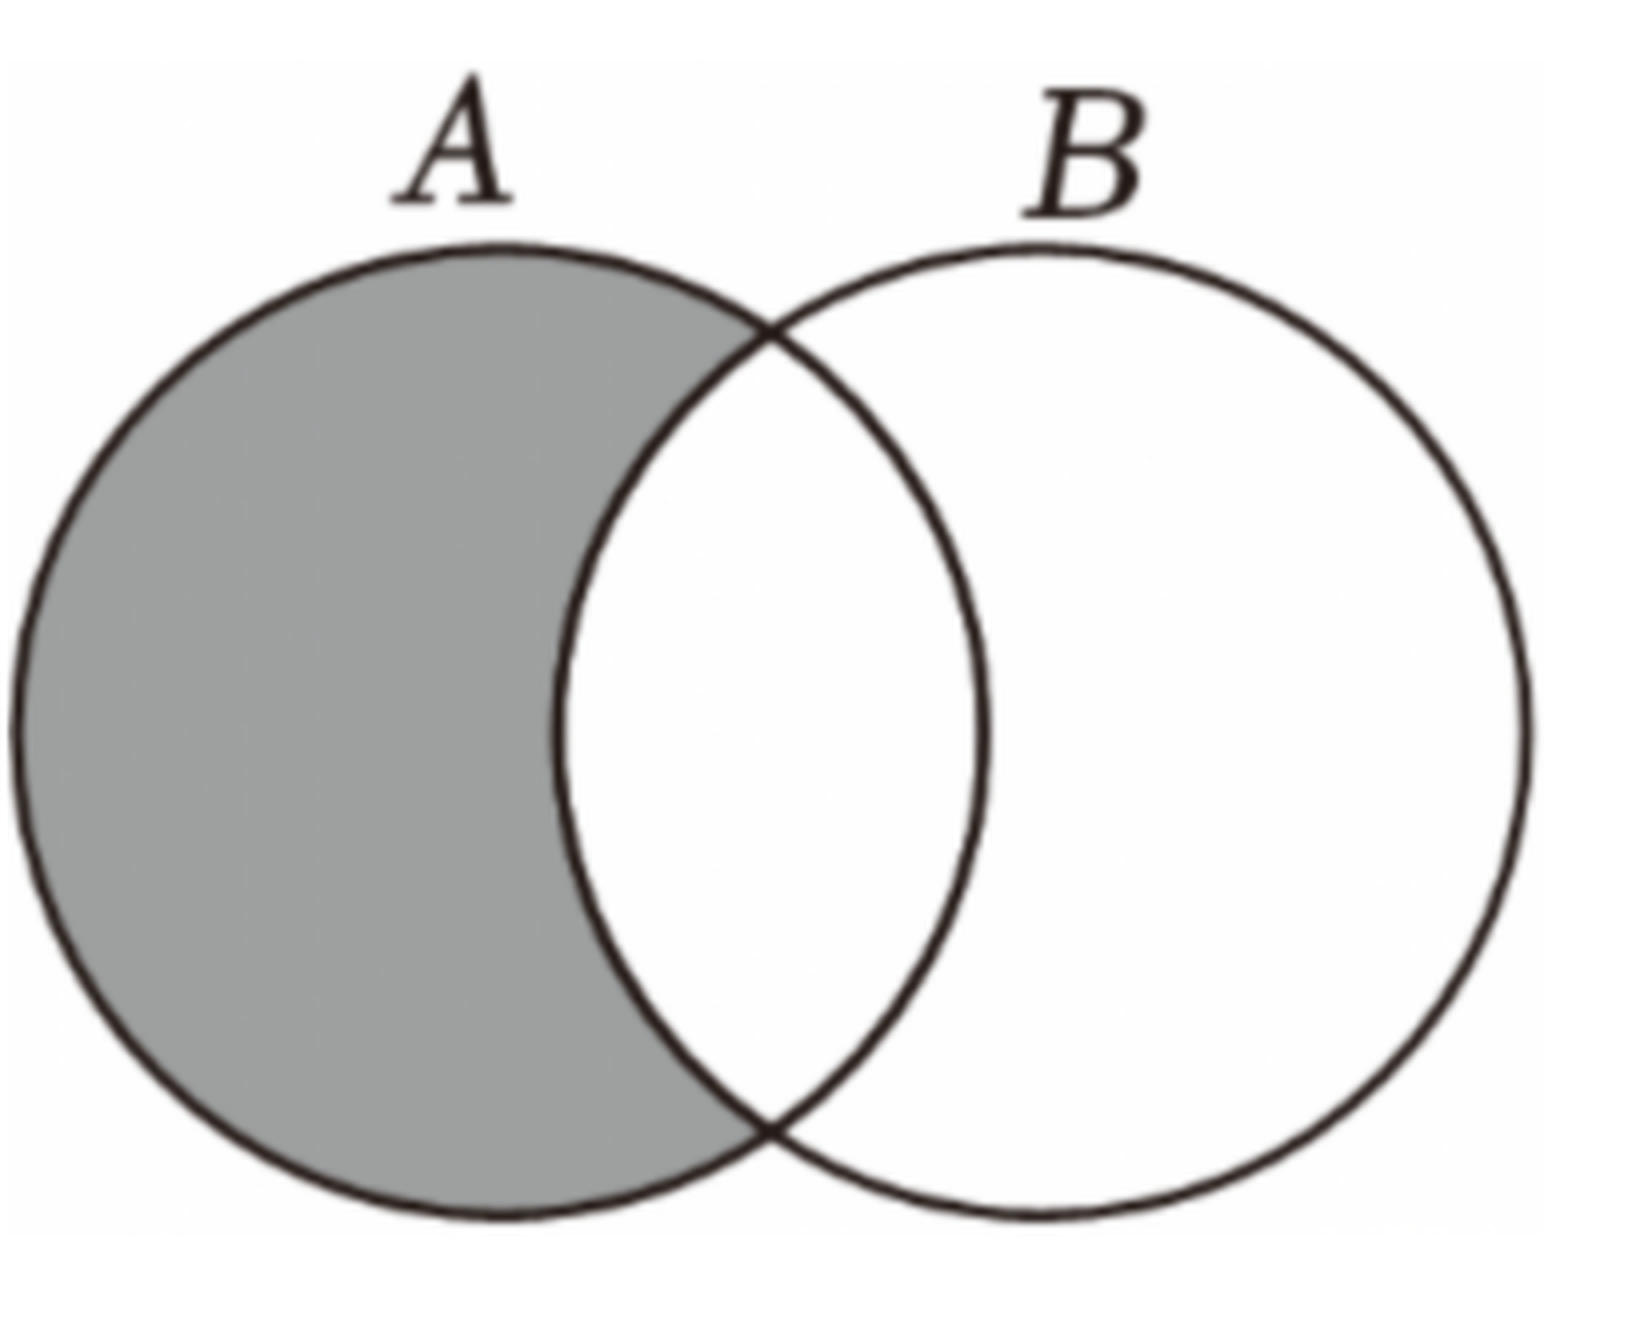
\includegraphics[width=0.30\textwidth]{figures/venn_A_minus_B_h38.png}
\end{center}

\ans{$\{1\}$}

\item 集合 $\{2,3,4,\cdots,2024,2025\}$ 的真子集的个数为 \blankline[4.4em].

\ans{$2^{2024}-1$}

\ifanswer
\solbegin
\step{集合 $\{2,3,4,\cdots,2024,2025\}$ 的真子集的个数为 $2^{2024}-1$.}
\solend

\fi

\item 已知集合 $A$ 中的元素都是正整数，其中最小的是 $1$，最大值是 $100$，除 $1$ 以外，每一个元
素都等于 $A$ 中的两个数（可以相同）的和，则集合 $A$ 中至少含有 \blankline[4.4em] 个元素.

\ans{$9$}

\ifanswer
\solbegin
\step{设 $A$ 中的数从小到大排列为 $1,a_1,a_2,\cdots,a_k,100$，}
\step{则 $a_1=1+1=2$；$3\leqslant a_2\leqslant 4$；$4\leqslant a_3\leqslant 8$；$5\leqslant a_4\leqslant 16$；$6\leqslant a_5\leqslant 32$；$7\leqslant a_6\leqslant 64$；}
\step{于是 $A$ 至少有八个数；}
\step{假设 $A$ 恰好有八个元素，由于 $a_5+a_6\leqslant 96<100$；}
\step{故必须有 $100=a_6+a_6$，$a_6=50$，}
\step{又 $a_4+a_5\leqslant 48$，同理 $a_5=25$，}
\step{但此时 $a_3+a_4\leqslant 24$，$a_5=2a_4$，$a_4=12.5$ 矛盾，}
\step{故 $A$ 不可能恰好有八个元素，因此 $A$ 至少有九个元素.}
\step{其九个数可以为 $1$，$2$，$3$，$6$，$12$，$13$，$25$，$50$，$100$.}
\solend

\fi

\item 已知集合 $\{x_1,x_2,x_3,x_4,x_5,x_6\}=\{1,2,3,4,5,6\}$，将 $x_i$ 与 $x_j$（其中 $i\in\{1,2,3\}$，
$j\in\{4,5,6\}$）的乘积 $x_ix_j$ 放入如图的 $3\times3$ 方格中，则方格中全部数之和的最大值为 \blankline[4.4em].

% 原卷的 $3\times3$ 方格是表格式内容（三行三列的公式），本稿按 高一03 的成例用 tabular 排出。
\begin{center}
\begin{tabular}{|c|c|c|}
\hline
$x_1x_4$ & $x_1x_5$ & $x_1x_6$ \\
\hline
$x_2x_4$ & $x_2x_5$ & $x_2x_6$ \\
\hline
$x_3x_4$ & $x_3x_5$ & $x_3x_6$ \\
\hline
\end{tabular}
\end{center}

\ans{$110$}

\ifanswer
\solbegin
\step{由表格数据得所有数之和为}
\step{$S=x_1x_4+x_1x_5+x_1x_6+x_2x_4+x_2x_5+x_2x_6+x_3x_4+x_3x_5+x_3x_6$，}
\step{所以 $S=(x_1+x_2+x_3)(x_4+x_5+x_6)$，}
\step{因为集合 $\{x_1,x_2,x_3,x_4,x_5,x_6\}=\{1,2,3,4,5,6\}$，}
\step{所以 $x_1+x_2+x_3+x_4+x_5+x_6=1+2+3+4+5+6=21$，}
\step{设 $t=x_1+x_2+x_3$，则 $6\leqslant t\leqslant 15$，$t\in\N^*$，}
\step{$S=t(21-t)=-\left(t-\dfrac{21}{2}\right)^2+\dfrac{441}{4}$，}
\step{当 $t=10$ 或 $t=11$ 时，$S=t(21-t)$ 取最大值，最大值为 $110$，}
\step{此时 $\{x_1,x_2,x_3\}=\{1,4,5\}$，$t=10$，所以可取最大值 $110$.}
\solend

\fi

\item 若 $[x]$ 表示不大于 $x$ 的最大整数，方程 $x^2-8[x]+7=0$ 的解集为 \blankline[4.4em].

\ans{$\{1,\sqrt{33},\sqrt{41},7\}$}

\ifanswer
\solbegin
\step{由题意，$x\geqslant[x]=\dfrac{x^2+7}{8}>0$，得 $x^2-8x+7\leqslant 0$，解得 $1\leqslant x\leqslant 7$，}
\step{$[x]=1$，$x^2=1$，$x=1$；}
\step{$[x]=2$，$x^2=9$，$x=3$ 与 $[x]=2$ 矛盾；}
\step{$[x]=3$，$x^2=17$，$x=\sqrt{17}$，$[x]=4$ 与 $[x]=3$ 矛盾；}
\step{$[x]=4$，$x^2=25$，$x=5$ 与 $[x]=4$ 矛盾；}
\step{$[x]=5$，$x^2=33$，$x=\sqrt{33}$，$[x]=5$；}
\step{$[x]=6$，$x^2=41$，$x=\sqrt{41}$，$[x]=6$；}
\step{$[x]=7$，$x^2=49$，$x=7$；}
\step{综上，方程 $x^2-8[x]+7=0$ 的解集为 $\{1,\sqrt{33},\sqrt{41},7\}$.}
\solend

\fi

\end{enumerate}

\bigsec{二、选择题}

\begin{enumerate}
\setcounter{enumi}{10}

\item 已知集合 $A=\{a,a^2\}$，$B=\{1,3\}$，若 $1\in A$，则 $A\cup B$ 中所有元素之和为\mbox{（\quad）}

\keepwithprev
A. $2$\qquad B. $3$\qquad C. $4$\qquad D. $5$

\ans{$B$}

\ifanswer
\solbegin
\step{因为 $1\in A$，集合 $A=\{a,a^2\}$，所以 $a=1$ 或 $a^2=1$，}
\step{若 $a=1$，则 $a=a^2$，与元素的互异性矛盾；}
\step{若 $a^2=1$，则 $a=1$（舍）或 $a=-1$，故 $A=\{-1,1\}$，$B=\{1,3\}$，}
\step{故 $A\cup B=\{-1,1,3\}$，所以 $A\cup B$ 中所有元素之和为 $-1+1+3=3$. 故选 $B$.}
\solend

\fi

\item 对于实数 $a$、$b$、$c$，下列命题正确的是\mbox{（\quad）}

\keepwithprev
A. 若 $a>b$，则 $ac^2>bc^2$\qquad B. 若 $a>b$，则 $a^2>b^2$

C. 若 $a>b$，则 $a|a|>b|b|$\qquad D. 若 $a>b>c>0$，则 $\dfrac{b}{a-b}<\dfrac{c}{a-c}$

\ans{$C$}

\ifanswer
\solbegin
\step{对于 $A$，若 $a>b$，$c=0$，则 $ac^2=bc^2$，故 $A$ 错误；}
\step{对于 $B$，若 $a>b$，取 $a=-1$，$b=-2$，则 $a^2<b^2$，故 $B$ 错误；}
\step{对于 $C$，若 $a>b>0$ 时，$a|a|-b|b|=a^2-b^2>0$，}
\step{当 $a>0>b$ 时，$a|a|-b|b|=a^2+b^2>0$，}
\step{当 $0>a>b$ 时，$a|a|-b|b|=b^2-a^2=(b-a)(b+a)>0$，}
\step{综上，若 $a>b$，则 $a|a|>b|b|$，故 $C$ 正确；}
\step{对于 $D$，若 $a>b>c>0$，$\dfrac{b}{a-b}-\dfrac{c}{a-c}=\dfrac{ab-bc-ac+bc}{(a-b)(a-c)}=\dfrac{a(b-c)}{(a-b)(a-c)}>0$，}
\step{故 $D$ 错误.}
\step{故选 $C$.}
\solend

\fi

\item 对于正整数集合 $A=\{a_1,a_2,\cdots,a_n\}(n\in\N^*,\ n\geqslant 3)$，如果去掉其中任意一个元素
$a_i(i=1,2,\cdots,n)$ 之后，剩余的所有元素组成的集合都能分为两个交集为空集的集合，且这
两个集合的所有元素之和相等，就称集合 $A$ 为平衡集. 记 $M=a_1+a_2+\cdots+a_n$. 若集合 $A$
是平衡集，并且存在 $a_i$ 为奇数，则集合 $A$ 中元素个数 $n$ 的奇偶性\mbox{（\quad）}

\keepwithprev
A. 与 $M$ 相关，既可以是奇数，又可以是偶数

B. 与 $M$ 无关，既可以是奇数，又可以是偶数

C. 与 $M$ 无关，必为偶数

D. 与 $M$ 无关，必为奇数

\ans{$D$}

\ifanswer
\solbegin
\step{正整数集合 $A=\{a_1,a_2,\cdots,a_n\}(n\in\N^*,\ n\geqslant 3)$，}
\step{因为集合 $A$ 是平衡集，设去掉元素 $a_i(i=1,2,\cdots,n)$，}
\step{由题意得 $A=A_1\cup A_2\cup\{a_i\}$，其中 $A_1\cap A_2=\varnothing$，}
\step{设集合 $A_1$ 和 $A_2$ 中的元素之和均为 $m$，所以 $M=2m+a_i$，其中 $i=1,2,\cdots,n$，}
\step{所以 $M-a_i=2m$，所以 $M-a_i$ 为偶数，其中 $i=1,2,\cdots,n$，}
\step{所以 $a_i(i=1,2,\cdots,n)$ 的奇偶性相同；}
\step{因为存在 $a_i$ 为奇数，所以 $a_i(i=1,2,\cdots,n)$ 均为奇数，}
\step{由 $M-a_i=2m$ 得 $M$ 也为奇数，且 $M=a_1+a_2+\cdots+a_n$，}
\step{所以 $n$ 也为奇数，所以 $n$ 必为奇数. 故选 $D$.}
\solend

\fi

\item 对于集合 $M=\{a\mid a=x^2-y^2,\ x\in\Z,\ y\in\Z\}$，给出如下三个结论：其中正确结论的个数
是\mbox{（\quad）}

\keepwithprev
①如果 $P=\{b\mid b=2n+1,\ n\in\Z\}$，那么 $P\sub M$；

②如果 $c=4n+2$，$n\in\Z$，那么 $c\notin M$；

③如果 $a_1\in M$，$a_2\in M$，那么 $a_1a_2\in M$.

\keepwithprev
A. $1$\qquad B. $2$\qquad C. $3$\qquad D. $0$

\ans{$C$}

\ifanswer
\solbegin
\step{对于①，$b=2n+1$，$n\in\Z$，则恒有 $2n+1=(n+1)^2-n^2$，}
\step{所以 $2n+1\in M$，即 $P=\{b\mid b=2n+1,n\in\Z\}$，则 $P\sub M$，①正确；}
\step{对于②，$c=4n+2$，$n\in\Z$，}
\step{若 $4n+2\in M$，则存在 $x$、$y\in\Z$ 使得 $x^2-y^2=4n+2$，}
\step{所以 $4n+2=(x+y)(x-y)$，又 $x+y$ 和 $x-y$ 同奇或同偶，}
\step{若 $x+y$ 和 $x-y$ 都是奇数，则 $(x+y)(x-y)$ 为奇数，而 $4n+2$ 是偶数；}
\step{若 $x+y$ 和 $x-y$ 都是偶数，则 $(x+y)(x-y)$ 能被 $4$ 整除，而 $4n+2$ 不能被 $4$ 整除，}
\step{所以 $4n+2\notin M$，即 $c\notin M$，②正确；}
\step{对于③，$a_1\in M$，$a_2\in M$，可设 $a_1=x_1^2-y_1^2$，$a_2=x_2^2-y_2^2$，$x_i$、$y_i\in\Z$；}
\step{则 $a_1a_2=(x_1^2-y_1^2)(x_2^2-y_2^2)=(x_1x_2)^2+(y_1y_2)^2-(x_1y_2)^2-(x_2y_1)^2$}
\step{$=(x_1x_2+y_1y_2)^2-(x_1y_2+x_2y_1)^2\in M$，那么 $a_1a_2\in M$，③正确.}
\step{综上，正确的命题是①②③. 故选 $C$.}
\solend

\fi

\end{enumerate}

\bigsec{三、解答题}

\begin{enumerate}
\setcounter{enumi}{14}

\item 已知 $A=\{x\mid a\leqslant x\leqslant -a+3\}$，$B=\{x\mid x<-1\text{ 或 }x>5\}$.

\begin{enumerate}[label=(\arabic*)]

\item 若 $A\cap B=\varnothing$，求 $a$ 的取值范围；

\item 若 $A\cup B=\R$，求 $a$ 的取值范围.

\end{enumerate}

\ans{（1）$[-1,+\infty)$；（2）$(-\infty,-2]$}

\ifanswer
\solbegin
\stepm{(1)}{①当 $A=\varnothing$ 时，$A\cap B=\varnothing$，需满足 $a>-a+3$，解得 $a>\dfrac32$，}
\step{故 $a$ 的取值范围为 $\left(\dfrac32,+\infty\right)$.}
\step{②当 $A\neq\varnothing$ 时，要使 $A\cap B=\varnothing$，需满足
$\begin{cases}a\leqslant\dfrac32\\[4pt] -a+3\leqslant 5\\[4pt] a\geqslant -1\end{cases}$，解得 $-1\leqslant a\leqslant\dfrac32$.}
\step{综上所述，$a$ 的取值范围是 $[-1,+\infty)$.}
\stepm{(2)}{因为 $A\cup B=\R$，$A=\{x\mid a\leqslant x\leqslant -a+3\}$，$B=\{x\mid x<-1\text{ 或 }x>5\}$，}
\step{所以 $\begin{cases}-a+3\geqslant 5\\[4pt] a\leqslant -1\end{cases}$，解得 $a\leqslant -2$，故所求 $a$ 的取值范围为 $(-\infty,-2]$.}
\solend

\fi

\ansspace[6]

\item 已知集合 $A=\{x\mid mx^2+x-2=0\}$，$B=\{x\mid 2x^2-5x-12=0\}$.

\begin{enumerate}[label=(\arabic*)]

\item 若 $A$ 中有且仅有 $1$ 个元素，求实数 $m$ 的值；

\item 已知集合 $C=A\cup B$，若 $C$ 的真子集有且仅有 $3$ 个，求实数 $m$ 的取值范围.

\end{enumerate}

\ans{（1）$m=0$ 或 $m=-\dfrac18$；（2）$\left\{m\mid m\leqslant -\dfrac18\right\}$}

\ifanswer
\solbegin
\stepm{(1)}{若 $m=0$，方程化为 $x-2=0$，此时方程有且仅有一个根 $x=2$；}
\step{若 $m\neq 0$，则 $\Delta=1^2-4\times m\times(-2)=0$，即 $m=-\dfrac18$ 时，}
\step{方程有两个相等的实根，此时集合 $A$ 中有且仅有一个元素，}
\step{所以实数 $m$ 的值为 $m=0$ 或 $m=-\dfrac18$；}
\stepm{(2)}{$B=\{x\mid 2x^2-5x-12=0\}=\left\{-\dfrac32,4\right\}$，}
\step{因为 $C=A\cup B$，若 $C$ 的真子集有且仅有 $3$ 个，则 $C$ 中有两个元素，}
\step{所以 $A\sub B$，由（1）得 $m=0$ 时，$A=\{2\}$，不符合 $A\sub B$，}
\step{当 $m\neq 0$ 时，若 $\Delta=1^2-4\times m\times(-2)<0$，解得 $m<-\dfrac18$，}
\step{此时 $A=\varnothing$，符合 $A\sub B$，}
\step{若 $\Delta=1^2-4\times m\times(-2)=0$，解得 $m=-\dfrac18$，}
\step{此时方程 $mx^2+x-2=0$ 的根为 $x=4$，集合 $A=\{4\}$，符合 $A\sub B$，}
\step{若 $\Delta=1^2-4\times m\times(-2)>0$，由 $A\sub B$，得 $A=\left\{-\dfrac32,4\right\}$，}
\step{此时有 $-\dfrac32+4=-\dfrac1m$ 且 $-\dfrac32\times 4=-\dfrac2m$，无解，}
\step{综上所述，实数 $m$ 的取值范围为 $\left\{m\mid m\leqslant -\dfrac18\right\}$.}
\solend

\fi

\ansspace[6]

\item 设 $A$ 是非空实数集，且 $0\notin A$. 若对于任意的 $x$、$y\in A$，都有 $xy\in A$，则称集合 $A$ 具
有性质 $P_1$；若对于任意的 $x$、$y\in A$，都有 $\dfrac xy\in A$，则称集合 $A$ 具有性质 $P_2$.

\begin{enumerate}[label=(\arabic*)]

\item 写出一个恰含有两个元素且具有性质 $P_1$ 的集合 $A$，并说明理由；

\item 证明：“非空实数集 $A$ 具有性质 $P_1$”是“非空实数集 $A$ 具有性质 $P_2$”的必要非充分条
件.

\end{enumerate}

\ans{（1）$A=\{-1,1\}$，理由见解析；（2）见解析}

\ifanswer
\solbegin
% 注：原卷本题 (1) 的解析里“证明”一词重复出现两次（一次接在分号后、一次另起一行），
%     本稿照原卷重复录入，未去重。
\stepm{(1)}{$A=\{-1,1\}$，证明：恰含有两个元素且具有性质 $P_1$ 的集合 $A=\{-1,1\}$；}
\step{证明：$1\times 1=1\in A$，$1\times(-1)=-1\in A$，$-1\times 1=-1\in A$，$-1\times(-1)=1\in A$；}
\stepm{(2)}{若集合 $A$ 具有性质 $P_2$，不妨设 $a\in A$，}
\step{由非空数集 $A$ 具有性质 $P_2$，有 $\dfrac aa=1\in A$.}
\step{①$A=\{1\}$，易得此时集合 $A$ 具有性质 $P_1$.}
\step{②数集 $A$ 只含有两个元素，不妨设 $A=\{1,a_1\}$，}
\step{由 $\dfrac{1}{a_1}=a_1$，且 $a_1\neq 1$，解得 $a_1=-1$，此时集合 $A$ 具有性质 $P_1$.}
\step{③实数集 $A$ 含有两个以上的元素，不妨设不为 $1$ 的元素 $a_1$、$a_2\in A$，}
\step{则有 $\dfrac{1}{a_1}\in A$，由于集合 $A$ 具有性质 $P_2$，}
\step{所以有 $a_2\div\dfrac{1}{a_1}=a_1a_2\in A$，这说明集合 $A$ 具有性质 $P_1$.}
\step{综上，若非空实数集 $A$ 具有性质 $P_2$，则集合 $A$ 具有性质 $P_1$，}
\step{所以“非空实数集 $A$ 具有性质 $P_1$”是“非空实数集 $A$ 具有性质 $P_2$”的}
\step{必要条件.}
\step{取正偶数集 $A=\{x\mid x=2n,\ n\in\N^*\}$，}
\step{对任意的 $2m$、$2n\in A$，$m$、$n\in\N^*$，}
\step{有 $2m\times 2n=4mn\in A$，故 $A$ 具有性质 $P_1$，}
\step{取 $x=2$，$y=4$，则 $\dfrac xy=\dfrac12\notin A$，故 $A$ 不具有性质 $P_2$，}
\step{所以“非空实数集 $A$ 具有性质 $P_1$”不是“非空实数集 $A$ 具有性质 $P_2$”的}
\step{充分条件.}
\step{综上，“非空实数集 $A$ 具有性质 $P_1$”是“非空实数集 $A$ 具有性质 $P_2$”的}
\step{必要非充分条件.}
\solend

\fi

\ansspace[8]

\item 已知命题 $p$：关于 $x$ 的方程 $x^2+mx+1=0$ 有两个不同的正根；命题 $q$：关于 $x$ 的方程
$4x^2+4(m-2)x=-1$ 有实根.

\begin{enumerate}[label=(\arabic*)]

\item 若命题 $q$ 为假命题，求整数 $m$ 的解集；

\item 若命题 $p$ 为真命题，且关于 $x$ 的方程 $x^2+mx+1=0$ 的两个实数根 $x_1$、$x_2$ 满足
$3x_1+2x_2=5$，求实数 $m$ 的取值集合；

\item 若命题 $p$ 和命题 $q$ 有且仅有一个成立，求实数 $m$ 的取值范围.

\end{enumerate}

\ans{（1）$\{2\}$；（2）$\left\{-\dfrac{13}{6}\right\}$；（3）$[-2,1]\cup[3,+\infty)$}

\ifanswer
\solbegin
\stepm{(1)}{命题 $q$：关于 $x$ 的方程 $4x^2+4(m-2)x=-1$ 有实根为假命题，}
\step{即 $4x^2+4(m-2)x+1=0$ 无实根，}
\step{则 $\Delta=16(m-2)^2-16<0$，则 $1<m<3$，则整数 $m$ 的解集为 $\{2\}$；}
\stepm{(2)}{若命题 $p$ 为真命题，且关于 $x$ 的方程 $x^2+mx+1=0$ 的两个实数根 $x_1$、$x_2$，}
\step{满足 $3x_1+2x_2=5$，则方程 $x^2+mx+1=0$ 有两个不同的正根，}
\step{则 $\begin{cases}\Delta=m^2-4>0\\[4pt] x_1+x_2=-m>0\end{cases}$，则 $m<-2$，}
\step{又 $\begin{cases}x_1+x_2=-m\\[4pt] x_1x_2=1\\[4pt] 3x_1+2x_2=5\end{cases}$，
则 $\begin{cases}x_1=5+2m\\[4pt] x_2=-3m-5\end{cases}$，则 $(5+2m)(-3m-5)=1$，}
\step{得 $m=-2$ 或 $m=-\dfrac{13}{6}$，又因为 $m<-2$，所以 $m=-\dfrac{13}{6}$，}
\step{所以实数 $m$ 的取值集合为 $\left\{-\dfrac{13}{6}\right\}$；}
\stepm{(3)}{由（2）得当 $p$ 为真时，则有 $m<-2$，}
\step{当 $q$ 为真时，$\Delta=16(m-2)^2-16\geqslant 0$，解得 $m\leqslant 1$ 或 $m\geqslant 3$，}
\step{又因为命题 $p$ 和命题 $q$ 只有一个为真，所以
$\begin{cases}m<-2\\[4pt] 1<m<3\end{cases}$ 或 $\begin{cases}m\geqslant -2\\[4pt] m\leqslant 1\text{ 或 }m\geqslant 3\end{cases}$，}
\step{解得 $-2\leqslant m\leqslant 1$ 或 $m\geqslant 3$，所以实数 $m$ 的取值范围为 $[-2,1]\cup[3,+\infty)$.}
\solend

\fi

\ansspace[8]

% 注：原卷此处作“设 $n\in\N^*$，集合含有 $3n$ 个元素”，**漏了符号 $U$**（应作“集合 $U$
%     含有 $3n$ 个元素”）——$U$ 直到本句末尾“则称 $U$ 为三分集合”才出现、此前无定义。
%     本稿照录未补，见文件头“原卷笔误/存疑”⑦。
\item 设 $n\in\N^*$，集合含有 $3n$ 个元素，若存在三个 $n$ 元集合 $A$、$B$、$C$ 满足如下两个条件，
则称 $U$ 为三分集合.

①$U=A\cup B\cup C$；

②$A$、$B$、$C$ 元素可分别排列为有序数组 $(a_1,a_2,\cdots,a_n)$，$(b_1,b_2,\cdots,b_n)$ 及
$(c_1,c_2,\cdots,c_n)$，使得对 $\forall i=1,2,\cdots,n$，均有 $a_i+b_i=c_i$.

特别地，当 $U=\{1,2,3,4,\cdots,3n-2,3n-1,3n\}$ 为三分集合时，称 $n$ 为完美三分数.

如：因为 $U=\{1,2,3\}$ 为三分集合，所以 $n=1$ 为最小完美三分数.

\begin{enumerate}[label=(\arabic*)]

\item 请判断下列两个集合是否为三分集合（直接写出结论）：

$U_1=\{1,2,3,4,5,6\}$，$U_2=\{1,3,5,7,8,9,10,11,12\}$；

\item 求出大于 $1$ 的最小完美三分数；

\item 请判断是否存在无穷多个完美三分数？若存在，请说明理由；若不存在，则求出最大的
完美三分数.

\end{enumerate}

\ans{（1）$U_1$ 不是三分集合，$U_2$ 是三分集合；（2）$4$；（3）存在，理由见解析}

\ifanswer
\solbegin
\stepm{(1)}{(i)$U_1=\{1,2,3,4,5,6\}$ 不是三分集合，下面用反证法证明：}
\step{证明：假设 $U=\{1,2,3,4,5,6\}$ 是三分集合，}
\step{设 $A=\{a_1,a_2\}$，$B=\{b_1,b_2\}$，$C=\{c_1,c_2\}$，不妨设 $c_1<c_2$，}
\step{因为 $a_1+b_1=c_1$，$a_2+b_2=c_2$，}
\step{所以 $a_1+b_1+a_2+b_2+c_1+c_2=2(c_1+c_2)=1+2+3+4+5+6=21$，}
% 注：原卷此步印“所以 $c_1+c_2=2$”，与上一行的 $2(c_1+c_2)=21$ **不自洽**
%     （应作 $\dfrac{21}2$）；同题 $n=3$ 处的同型推理原卷写的是 $\dfrac{45}2$，故此处是原卷笔误。
%     本稿照录未改，见文件头“原卷笔误/存疑”⑧。
\step{所以 $c_1+c_2=2$，这与 $c_1,c_2\in\N^*$ 矛盾，故假设错误，}
\step{故 $U_1=\{1,2,3,4,5,6\}$ 不是三分集合；}
\step{(ii)$U_2=\{1,3,5,7,8,9,10,11,12\}$ 是三分集合，理由如下：}
\step{令 $A=\{1,3,5\}$，$B=\{9,8,7\}$，$C=\{10,11,12\}$，}
\step{则 $A\cup B\cup C=U=\{1,3,5,7,8,9,10,11,12\}$，满足条件①；}
\step{又 $1+9=10$；$3+8=11$；$5+7=12$，所以满足条件②，}
\step{所以 $U_2=\{1,3,5,7,8,9,10,11,12\}$ 是三分集合；}
\stepm{(2)}{由（1）得，当 $n=2$ 时，$U=\{1,2,3,4,5,6\}$ 不是三分集合；}
\step{当 $n=3$ 时，$U=\{1,2,3,4,5,6,7,8,9\}$，}
\step{假设 $U=\{1,2,3,4,5,6,7,8,9\}$ 是三分集合，}
\step{同理由 $a_1+b_1+a_2+b_2+a_3+b_3+c_1+c_2+c_3$}
\step{$=2(c_1+c_2+c_3)=1+2+\cdots+9=45$，$c_1+c_2+c_3=\dfrac{45}{2}$，}
\step{可推出与 $c_1$、$c_2$、$c_3\in\N^*$ 矛盾，故假设也错误，}
\step{所以 $U=\{1,2,3,4,5,6,7,8,9\}$ 不是三分集合；}
\step{当 $n=4$ 时，$U=\{1,2,3,\cdots,12\}$，}
\step{存在三个 $4$ 元集合 $A=\{1,2,4,3\}$，$B=\{5,8,7,9\}$，$C=\{6,10,11,12\}$，}
\step{满足 $U=\{1,2,3,\cdots,12\}$ 为三分集合的两个条件，}
\step{故大于 $1$ 的最小完美三分数为 $4$；}
\stepm{(3)}{存在无穷多个完美三分数，理由如下：}
\step{由题意得，$n=1$ 为最小完美三分数，}
\step{当 $n=5$ 时，$U=\{1,2,3,\cdots,15\}$，}
\step{存在三个 $5$ 元集合 $A=\{1,3,5,7,2\}$，$B=\{11,10,9,8,4\}$，$C=\{12,13,14,15,6\}$，}
\step{满足三分集合的条件，故 $5$ 为完美三分数；}
\step{当 $n=21$ 时，$U=\{1,2,3,\cdots,63\}$，}
\step{存在如下三个 $21$ 元的集合满足三分集合的条件：}
\step{$A=\{1,3,5,7,\cdots,29,31,2,6,10,14,4\}$，}
\step{$B=\{47,46,45,44,\cdots,33,32,22,20,18,16,8\}$，}
\step{$C=\{48,49,50,51,\cdots,62,63,24,26,28,30,12\}$，}
\step{故 $21$ 为完美三分数.}
\step{首先证明：若 $n=k$，$k\in\N^*$ 为三分完美数，}
\step{则 $n=4k+1$，$k\in\N^*$ 也为三分完美数，}
% 注：下一行原卷印作“$U_{k+1}=U_{k+1}=\{2,3,\cdots,12k+3\}$”——等号两边记号相同，
%     依上下文疑当作 $U'_{k+1}=U_{4k+1}$，且此处集合自 2 起（前文 $U_{4k+1}$ 自 1 起）；
%     本稿照录原卷，未代为改写。
\step{证明：记 $U_k=\{1,2,3,\cdots,3k\}$，$U_{4k+1}=\{1,2,3,\cdots,12k+3\}$，}
\step{若 $n=k$，$k\in\N^*$ 为三分完美数，则 $U_k$ 为三分集合，}
\step{即存在三个 $k$ 元集合 $A$、$B$、$C$ 满足如下两个条件，}
\step{①$U_k=A\cup B\cup C$；}
\step{②$A$、$B$、$C$ 元素可分别排列为有序数组 $(a_1,a_2,\cdots,a_k)$，}
\step{$(b_1,b_2,\cdots,b_k)$ 及 $(c_1,c_2,\cdots,c_k)$，}
\step{使得对 $\forall i=1,2,3,\cdots,k$，均有 $a_i+b_i=c_i$，}
\step{则可得到对 $\forall i=1,2,3,\cdots,k$，$2a_i+2b_i=2c_i$，}
\step{故集合 $\{2,4,6,\cdots,6k\}$ 也满足三分集合的两个条件，其也为三分集合，}
\step{下面记集合 $\{2,4,6,\cdots,6k\}=2U_k$，}
\step{对 $n=4k+1$，集合 $U_{k+1}=U_{k+1}=\{2,3,\cdots,12k+3\}=(2U_k)\cup\complement_{U_{4k+1}}(2U_k)$，}
\step{构造集合 $A'=\{1,3,5,7,\cdots,6k+1\}$，共有 $3k+1$ 个奇数；}
% 注：下一行原卷印作“$B'=\{6k+3k+2,6k+3k+1,6k+3k,6k+3k-1,\cdots,6k+2\}$”，
%     按与后文 $C'$ 相接，前四项当写作 $9k+2$、$9k+1$、$9k$、$9k-1$；本稿照录原卷。
\step{集合 $B'=\{6k+3k+2,6k+3k+1,6k+3k,6k+3k-1,\cdots,6k+2\}$，}
\step{共有 $3k+1$ 个逐个减小的连续正整数；}
\step{集合 $C'=\{9k+3,9k+4,9k+5,9k+6,\cdots,12k+3\}$，}
\step{共有 $3k+1$ 个逐个增大的连续正整数；}
\step{得这三个 $3k+1$ 元集合 $A'$、$B'$、$C'$ 满足如下两个条件，}
\step{①集合 $A'\cup B'\cup C'=\complement_{U_{4k+1}}(2U_k)$；}
\step{②$A'$、$B'$、$C'$ 元素可分别排列为有序数组 $(a_1,a_2,\cdots,a_{3k+1})$，}
\step{$(b_1,b_2,\cdots,b_{3k+1})$ 及 $(c_1,c_2,\cdots,c_{3k+1})$，}
\step{使得对 $\forall i=1,2,3,\cdots,3k+1$，均有 $a_i+b_i=c_i$；}
\step{故 $\complement_{U_{4k+1}}(2U_k)$ 为三分集合，而已知 $U_k$ 为三分集合，}
\step{将其对应与 $A'$、$B'$、$C'$ 合并，}
% 注：原卷此处印“令 $A''=A\cup A'$”（$B''$、$C''$ 同）。按同段上文“记集合
%     $\{2,4,6,\cdots,6k\}=2U_k$”，此处疑当作 $A''=2A\cup A'$——否则
%     $A''\cup B''\cup C''=U_k\cup\complement_{U_{4k+1}}(2U_k)\neq U_{4k+1}$，与本段结论冲突。
%     本稿照录未改，见文件头“原卷笔误/存疑”⑨。
\step{令 $A''=A\cup A'$，$B''=B\cup B'$，$C''=C\cup C'$，}
\step{则这三个 $4k+1$ 元集合 $A''$、$B''$、$C''$，}
\step{满足 $A''\cup B''\cup C''=U_{4k+1}$，且满足条件②，}
\step{故 $U_{4k+1}=\{1,2,3,\cdots,12k+3\}$ 为三分集合，}
\step{因此可得，若 $n=k$ 为三分完美数，则 $n=4k+1$ 也为三分完美数，}
\step{由 $1$，$5$，$21$ 为完美三分数，结合所证结论得，存在无穷多个完美三分数.}
\solend

\fi

\ansspace*[12]

\end{enumerate}

\end{document}
"
% 紧凑版：xelatex "\def\iscompact{1}% 高一38_大同中学_周末作业3.tex
%   —— 高一上数学“2026-2027 年大同中学高一上周末作业 3”（试卷版/答案版）
% 试卷版：xelatex 高一38_大同中学_周末作业3.tex
% 答案版：xelatex "\def\isanswer{1}% 高一38_大同中学_周末作业3.tex
%   —— 高一上数学“2026-2027 年大同中学高一上周末作业 3”（试卷版/答案版）
% 试卷版：xelatex 高一38_大同中学_周末作业3.tex
% 答案版：xelatex "\def\isanswer{1}\input{高一38_大同中学_周末作业3.tex}"
% 紧凑版：xelatex "\def\iscompact{1}\input{高一38_大同中学_周末作业3.tex}"
%
% 原始材料是微信公众号图文（公众号“魔都数学加油站”连载“27学年高一 38”，署名“破晓”，
% 2026-09-26 21:29 发布，原文标题“27学年高一38——2026-2027年上海市大同中学高一上周末作业3”，
% 原文链接 https://mp.weixin.qq.com/s/O_O60vCIiGi2xponAo4irw ），正文为 12 张 PNG 页。
% **同一篇里各页分辨率不一致**（2560×3620 与 4762×6735 两档混排：第 1、10、11、12 页为
% 2560×3620，第 2—9 页为 4762×6735）。原文本身就是一份**讲评版**——有的题下方只印
% 【答案】行，有的只印【解析】。试题文字、答案与解析均照原卷录入，未改内容。卷面的粉色
% 斜水印“魔都数学加油站”属水印，未录入。
%
% 本卷共 **17 题**：填空题 8 题（第 3—10 题）、选择题 4 题（第 11—14 题）、解答题 5 题
% （第 15—19 题）；插图 1 张（第 6 题 Venn 图）。三版页数：试卷版 4 页 / 答案版 11 页 /
% 紧凑版 3 页，`Overfull`／`Underfull`／`Missing character` 告警均为 0。
%
% 卷首标题：原卷印作“2026-2027 年大同中学高一上周末作业 3”（公众号原文标题里的“上海市”
% 三字卷面标题行没有，本稿照卷面），年份区间按全稿惯例排 en dash，前缀照原卷保留“年”。
%
% 与原卷的排版差异（均已在 README“说明”中交代）：
%   ① 原文自**第 3 题**起（第 1、2 题未在该文中发布），故本稿题号亦自 3 起，填空题以
%      \setcounter{enumi}{2} 起编；选择、解答两节各按上一节末号另设 \setcounter
%      （选择题 \setcounter{enumi}{10}、解答题 \setcounter{enumi}{14}）；
%   ② 原卷本就印有“一、填空题”“二、选择题”“三、解答题”三节标题，本稿照原卷分节，
%      只把标题改排成全稿统一的“大节标题”样式；
%   ③ 原卷是“讲评版”：第 3、6 题只印【答案】行，第 4、5、7、8、9、10 题与第 11—19 题印
%      【解析】；本稿统一改为试卷版隐去、答案版以 \ans{}／\ifanswer 块给出，两版彻底分离。
%      其中第 4、5、7、8、9、10 题与第 11—14 题的答案，原卷写在【解析】末句，本稿另提为
%      \ans{}；第 15—19 题原卷只有【解析】、无独立答案行，本稿亦补了摘要式 \ans{}。
%      **故本卷 17 题每题都有 \ans**——比“只印【解析】的填空、解答题不另提 \ans”的
%      高一31／高一34 更彻底，与 高一21 第 11 题（填空，答案在【解析】末句，本稿另提）同类；
%      （本仓对“另提 \ans{}”的做法各卷不一，见 README 对应专记的核对面。）
%   ④ 数集记号原卷两套并用：第 3、5 题的实数集作粗体 $\mathbf{R}$，第 8、14、17、18 题等的
%      整数集、自然数集作斜体 $Z$、$N$，本稿按全稿惯例统一写作 $\R$、$\Z$、$\N$；
%   ⑤ 原卷填空的横线宽度不一（约 1.8—3.6 字宽），本稿按全稿惯例统一排 \blankline[4.4em]；
%   ⑥ 中文括注原卷用半角“(  )”，本稿按全稿惯例排全角；选择题的作答括注统一排
%      \mbox{（\quad）}（第 14 题的作答括注原卷印在 ①②③ 三个命题**之前**，本稿照原卷次序）；
%      数学式内部的括注（如第 4 题的 $p\%(0<p<100)$、第 13 题的 $a_i(i=1,2,\cdots,n)$）照原样
%      留在行内公式里，未改全角；
%   ⑦ 原卷并列的字母（“x,y”“a,b,c”）不加标点或作半角逗号，本稿按全稿惯例改排顿号；
%   ⑧ 第 6 题的 Venn 图取原卷截图、4× LANCZOS 放大（figures/venn_A_minus_B_h38.png，
%      见该处 \includegraphics 前的注释）；第 9 题的 $3\times3$ 方格属**表格式**内容，
%      本稿按 高一03 的成例用 tabular 排出，未截图；
%   ⑨ 原卷未印副标题，本稿按**本卷实际内容**补出副标题“集合与常用逻辑用语”（依据见下条）；
%   ⑩ 原卷【解析】**一个印刷行照录为一条 `\step`**（原卷的折行也照录为独立一条，如第 17 题
%      末三处“…的”／“必要条件.”这类跨行句、第 9 题“由表格数据得所有数之和为”／
%      “$S=\cdots$，”），使答案版的排布与原卷讲评版逐行对应；全卷 15 处【解析】合计
%      **191 条 `\step` ＝ 原卷 191 行**（逐处：5、5、1、9、9、9、4、9、9、12、6、14、21、13、65）。
%
% 副标题（\examtitlest 第二个参数）：本卷卷面未印副标题，由本稿补出，取值按 2026-09-26 起的
%   新口径“只用本卷实际内容的模块名”定为“集合与常用逻辑用语”。依据：全卷 17 题
%   （第 3—19 题）中，第 3、5、6、7、8、9、10、11、13、14、15、16、17、18、19 题共 15 题
%   是集合的运算与关系、子集计数、集合新定义（性质 $P_1$／$P_2$、平衡集、三分集合），以及
%   命题与逻辑（第 3 题即用反证法证明“$x+y>2\Rightarrow x>1$ 或 $y>1$”这一命题）；不等式只
%   出现在第 4 题（降价提价的应用比较）、第 12 题（不等式命题真假）与第 10 题解析里解一元
%   二次不等式，合计不足全卷的三分之一，故不并标“不等式”。
%
% 原卷笔误/存疑（均照抄原卷、未改，见源码中该处上方注释）：
%   ① 第 19 题 (3) 的证明里印作“集合 $U_{k+1}=U_{k+1}=\{2,3,\cdots,12k+3\}$”——等号两边
%      记号相同（依上下文疑当作 $U'_{k+1}=U_{4k+1}$），且此处集合自 $2$ 起，而前文
%      $U_{4k+1}=\{1,2,3,\cdots,12k+3\}$ 自 $1$ 起；本稿照录；
%   ② 第 19 题 (3) 的证明里印作
%      “$B'=\{6k+3k+2,6k+3k+1,6k+3k,6k+3k-1,\cdots,6k+2\}$”——按与后文
%      $C'=\{9k+3,9k+4,9k+5,9k+6,\cdots,12k+3\}$ 相接，前四项当写作 $9k+2$、$9k+1$、
%      $9k$、$9k-1$（即 $6k+3k+2$ 等），原卷即作“$6k+3k+\cdots$”形式，本稿照录；
%   ③ 第 19 题的术语前后不一：题干与 (1)(2)(3) 用“完美三分数”，而 (3) 的证明里五次写作
%      “三分完美数”（词序不同）；本稿五处都照录；
%   ④ 第 14 题题干作“给出如下三个结论：其中正确结论的个数是（\quad）”，此处冒号疑当作
%      逗号，本稿照录；
%   ⑤ 第 17 题题干作“非空实数集”，其解析有一处写作“非空数集”；本稿照录；
%   ⑥ 第 17 题 (1) 的【解析】原卷连写“…集合 $A=\{-1,1\}$；证明：…；证明：…”，“证明”
%      一词重复出现两次（第一次在分行处、第二次另起一行），本稿照原卷重复录入，未去重。
%   ⑦ 第 19 题**题干漏字**：原卷作“19.设 $n\in\N^*$，集合含有 $3n$ 个元素…则称 $U$ 为
%      三分集合”——首句漏了符号 $U$（应作“集合 $U$ 含有 $3n$ 个元素”），$U$ 直到结论句
%      才出现、此前无定义；本稿照录未补（见该处上方注释）。
%   ⑧ 第 19(1)(i) 的【解析】**自相矛盾**：上一行印“$a_1+b_1+a_2+b_2+c_1+c_2=2(c_1+c_2)
%      =1+2+3+4+5+6=21$”，下一行却印“所以 $c_1+c_2=2$”（由 $2(c_1+c_2)=21$ 应得
%      $c_1+c_2=\dfrac{21}2$，非整数、才与 $c_1,c_2\in\N^*$ 矛盾）；同题 $n=3$ 处的同型
%      推理原卷就写对了（$\dfrac{45}2$），故此处是原卷笔误；本稿照录未改（见该处上方注释）。
%   ⑨ 第 19(3) 的【解析】印“令 $A''=A\cup A'$，$B''=B\cup B'$，$C''=C\cup C'$”——按同段
%      上文“记集合 $\{2,4,6,\cdots,6k\}=2U_k$”，$A''$ 等疑当作 $2A\cup A'$（$B''$、$C''$ 同），
%      否则 $A''\cup B''\cup C''=U_k\cup\complement_{U_{4k+1}}(2U_k)\neq U_{4k+1}$；本稿照录未改
%      （见该处上方注释）。

\documentclass[a4paper,11pt]{article}
\usepackage{common}

\begin{document}

\examtitlest[3]{2026--2027 年大同中学高一上周末作业 3}{集合与常用逻辑用语}

\bigsec{一、填空题}

\begin{enumerate}
% 原卷填空题自第 3 题起（第 1、2 题未在该文中发布），须与选择、解答两节的 \setcounter 对齐
\setcounter{enumi}{2}

\item 设 $x$、$y\in\R$，若 $x+y>2$，则 $x>1$ 或 $y>1$ 是真命题. 这个命题可以用反证法去证明，
可以假设：\blankline[4.4em].

\ans{$x\leqslant 1$ 且 $y\leqslant 1$}

\item 已知某商品的原价为 $a$ 元，由于市场原因，先降价 $p\%(0<p<100)$ 出售，一段时间后，
再提价 $p\%$ 出售，则该商品提价后的售价 \blankline[4.4em] 该商品的原价（填“高于”“低于”或“等于”）.

\ans{低于}

\ifanswer
\solbegin
\step{由题意得第一次降价后的售价为 $a(1-p\%)$ 元，}
\step{第二次提价后的售价为 $a(1-p\%)(1+p\%)$ 元，}
\step{因为 $0<p<100$，所以 $0<p\%<1$，}
\step{因为 $a(1-p\%)(1+p\%)=a[1-(p\%)^2]<a$，}
\step{即该商品提价后的售价低于该商品的原价.}
\solend

\fi

\item 若集合 $A=\{x\mid ax^2+ax+1=0,\ a\in\R,\ x\in\R\}$ 的子集只有两个，则实数 $a=$ \blankline[4.4em].

\ans{$4$}

\ifanswer
\solbegin
\step{集合 $A=\{x\mid ax^2+ax+1=0\}$ 的子集只有两个，}
\step{所以 $A$ 有且只有一个元素，}
\step{①若 $a=0$，则 $A=\varnothing$ 不成立；}
\step{②若 $a\neq 0$，则 $\Delta=a^2-4a=0$，解得 $a=4$（$0$ 舍）.}
\step{故 $a=4$.}
\solend

\fi

\item 如图，已知集合 $A=\{1,2,3,4,5\}$，集合 $B=\{2,3,4,5,9\}$，则图中阴影部分所表示的
集合为 \blankline[4.4em].

% 图取原卷截图（01.png，2560×3620）右栏，4× LANCZOS 放大；为避免与 高一11 的
% figures/venn_A_minus_B.png 同名，按 高一32 的成例加 _h38 后缀。
\begin{center}
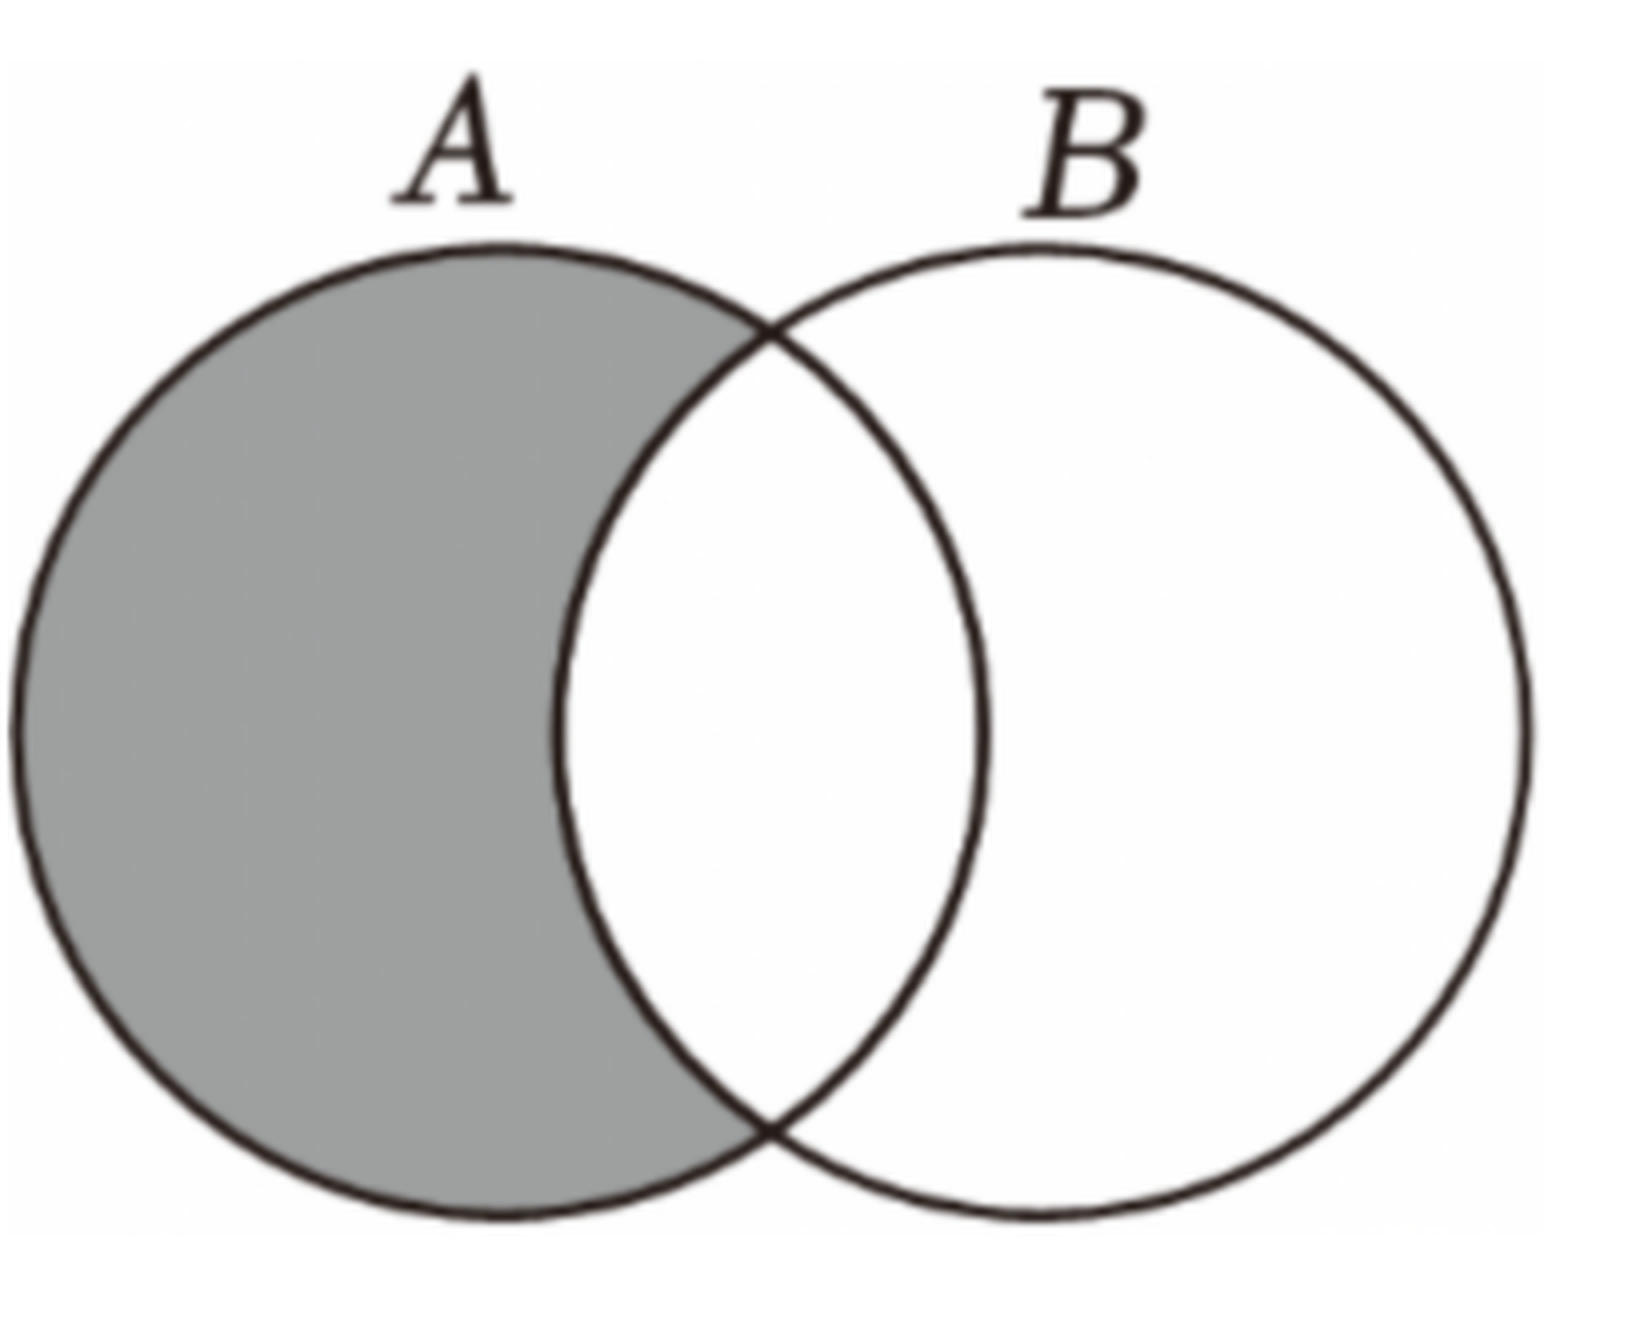
\includegraphics[width=0.30\textwidth]{figures/venn_A_minus_B_h38.png}
\end{center}

\ans{$\{1\}$}

\item 集合 $\{2,3,4,\cdots,2024,2025\}$ 的真子集的个数为 \blankline[4.4em].

\ans{$2^{2024}-1$}

\ifanswer
\solbegin
\step{集合 $\{2,3,4,\cdots,2024,2025\}$ 的真子集的个数为 $2^{2024}-1$.}
\solend

\fi

\item 已知集合 $A$ 中的元素都是正整数，其中最小的是 $1$，最大值是 $100$，除 $1$ 以外，每一个元
素都等于 $A$ 中的两个数（可以相同）的和，则集合 $A$ 中至少含有 \blankline[4.4em] 个元素.

\ans{$9$}

\ifanswer
\solbegin
\step{设 $A$ 中的数从小到大排列为 $1,a_1,a_2,\cdots,a_k,100$，}
\step{则 $a_1=1+1=2$；$3\leqslant a_2\leqslant 4$；$4\leqslant a_3\leqslant 8$；$5\leqslant a_4\leqslant 16$；$6\leqslant a_5\leqslant 32$；$7\leqslant a_6\leqslant 64$；}
\step{于是 $A$ 至少有八个数；}
\step{假设 $A$ 恰好有八个元素，由于 $a_5+a_6\leqslant 96<100$；}
\step{故必须有 $100=a_6+a_6$，$a_6=50$，}
\step{又 $a_4+a_5\leqslant 48$，同理 $a_5=25$，}
\step{但此时 $a_3+a_4\leqslant 24$，$a_5=2a_4$，$a_4=12.5$ 矛盾，}
\step{故 $A$ 不可能恰好有八个元素，因此 $A$ 至少有九个元素.}
\step{其九个数可以为 $1$，$2$，$3$，$6$，$12$，$13$，$25$，$50$，$100$.}
\solend

\fi

\item 已知集合 $\{x_1,x_2,x_3,x_4,x_5,x_6\}=\{1,2,3,4,5,6\}$，将 $x_i$ 与 $x_j$（其中 $i\in\{1,2,3\}$，
$j\in\{4,5,6\}$）的乘积 $x_ix_j$ 放入如图的 $3\times3$ 方格中，则方格中全部数之和的最大值为 \blankline[4.4em].

% 原卷的 $3\times3$ 方格是表格式内容（三行三列的公式），本稿按 高一03 的成例用 tabular 排出。
\begin{center}
\begin{tabular}{|c|c|c|}
\hline
$x_1x_4$ & $x_1x_5$ & $x_1x_6$ \\
\hline
$x_2x_4$ & $x_2x_5$ & $x_2x_6$ \\
\hline
$x_3x_4$ & $x_3x_5$ & $x_3x_6$ \\
\hline
\end{tabular}
\end{center}

\ans{$110$}

\ifanswer
\solbegin
\step{由表格数据得所有数之和为}
\step{$S=x_1x_4+x_1x_5+x_1x_6+x_2x_4+x_2x_5+x_2x_6+x_3x_4+x_3x_5+x_3x_6$，}
\step{所以 $S=(x_1+x_2+x_3)(x_4+x_5+x_6)$，}
\step{因为集合 $\{x_1,x_2,x_3,x_4,x_5,x_6\}=\{1,2,3,4,5,6\}$，}
\step{所以 $x_1+x_2+x_3+x_4+x_5+x_6=1+2+3+4+5+6=21$，}
\step{设 $t=x_1+x_2+x_3$，则 $6\leqslant t\leqslant 15$，$t\in\N^*$，}
\step{$S=t(21-t)=-\left(t-\dfrac{21}{2}\right)^2+\dfrac{441}{4}$，}
\step{当 $t=10$ 或 $t=11$ 时，$S=t(21-t)$ 取最大值，最大值为 $110$，}
\step{此时 $\{x_1,x_2,x_3\}=\{1,4,5\}$，$t=10$，所以可取最大值 $110$.}
\solend

\fi

\item 若 $[x]$ 表示不大于 $x$ 的最大整数，方程 $x^2-8[x]+7=0$ 的解集为 \blankline[4.4em].

\ans{$\{1,\sqrt{33},\sqrt{41},7\}$}

\ifanswer
\solbegin
\step{由题意，$x\geqslant[x]=\dfrac{x^2+7}{8}>0$，得 $x^2-8x+7\leqslant 0$，解得 $1\leqslant x\leqslant 7$，}
\step{$[x]=1$，$x^2=1$，$x=1$；}
\step{$[x]=2$，$x^2=9$，$x=3$ 与 $[x]=2$ 矛盾；}
\step{$[x]=3$，$x^2=17$，$x=\sqrt{17}$，$[x]=4$ 与 $[x]=3$ 矛盾；}
\step{$[x]=4$，$x^2=25$，$x=5$ 与 $[x]=4$ 矛盾；}
\step{$[x]=5$，$x^2=33$，$x=\sqrt{33}$，$[x]=5$；}
\step{$[x]=6$，$x^2=41$，$x=\sqrt{41}$，$[x]=6$；}
\step{$[x]=7$，$x^2=49$，$x=7$；}
\step{综上，方程 $x^2-8[x]+7=0$ 的解集为 $\{1,\sqrt{33},\sqrt{41},7\}$.}
\solend

\fi

\end{enumerate}

\bigsec{二、选择题}

\begin{enumerate}
\setcounter{enumi}{10}

\item 已知集合 $A=\{a,a^2\}$，$B=\{1,3\}$，若 $1\in A$，则 $A\cup B$ 中所有元素之和为\mbox{（\quad）}

\keepwithprev
A. $2$\qquad B. $3$\qquad C. $4$\qquad D. $5$

\ans{$B$}

\ifanswer
\solbegin
\step{因为 $1\in A$，集合 $A=\{a,a^2\}$，所以 $a=1$ 或 $a^2=1$，}
\step{若 $a=1$，则 $a=a^2$，与元素的互异性矛盾；}
\step{若 $a^2=1$，则 $a=1$（舍）或 $a=-1$，故 $A=\{-1,1\}$，$B=\{1,3\}$，}
\step{故 $A\cup B=\{-1,1,3\}$，所以 $A\cup B$ 中所有元素之和为 $-1+1+3=3$. 故选 $B$.}
\solend

\fi

\item 对于实数 $a$、$b$、$c$，下列命题正确的是\mbox{（\quad）}

\keepwithprev
A. 若 $a>b$，则 $ac^2>bc^2$\qquad B. 若 $a>b$，则 $a^2>b^2$

C. 若 $a>b$，则 $a|a|>b|b|$\qquad D. 若 $a>b>c>0$，则 $\dfrac{b}{a-b}<\dfrac{c}{a-c}$

\ans{$C$}

\ifanswer
\solbegin
\step{对于 $A$，若 $a>b$，$c=0$，则 $ac^2=bc^2$，故 $A$ 错误；}
\step{对于 $B$，若 $a>b$，取 $a=-1$，$b=-2$，则 $a^2<b^2$，故 $B$ 错误；}
\step{对于 $C$，若 $a>b>0$ 时，$a|a|-b|b|=a^2-b^2>0$，}
\step{当 $a>0>b$ 时，$a|a|-b|b|=a^2+b^2>0$，}
\step{当 $0>a>b$ 时，$a|a|-b|b|=b^2-a^2=(b-a)(b+a)>0$，}
\step{综上，若 $a>b$，则 $a|a|>b|b|$，故 $C$ 正确；}
\step{对于 $D$，若 $a>b>c>0$，$\dfrac{b}{a-b}-\dfrac{c}{a-c}=\dfrac{ab-bc-ac+bc}{(a-b)(a-c)}=\dfrac{a(b-c)}{(a-b)(a-c)}>0$，}
\step{故 $D$ 错误.}
\step{故选 $C$.}
\solend

\fi

\item 对于正整数集合 $A=\{a_1,a_2,\cdots,a_n\}(n\in\N^*,\ n\geqslant 3)$，如果去掉其中任意一个元素
$a_i(i=1,2,\cdots,n)$ 之后，剩余的所有元素组成的集合都能分为两个交集为空集的集合，且这
两个集合的所有元素之和相等，就称集合 $A$ 为平衡集. 记 $M=a_1+a_2+\cdots+a_n$. 若集合 $A$
是平衡集，并且存在 $a_i$ 为奇数，则集合 $A$ 中元素个数 $n$ 的奇偶性\mbox{（\quad）}

\keepwithprev
A. 与 $M$ 相关，既可以是奇数，又可以是偶数

B. 与 $M$ 无关，既可以是奇数，又可以是偶数

C. 与 $M$ 无关，必为偶数

D. 与 $M$ 无关，必为奇数

\ans{$D$}

\ifanswer
\solbegin
\step{正整数集合 $A=\{a_1,a_2,\cdots,a_n\}(n\in\N^*,\ n\geqslant 3)$，}
\step{因为集合 $A$ 是平衡集，设去掉元素 $a_i(i=1,2,\cdots,n)$，}
\step{由题意得 $A=A_1\cup A_2\cup\{a_i\}$，其中 $A_1\cap A_2=\varnothing$，}
\step{设集合 $A_1$ 和 $A_2$ 中的元素之和均为 $m$，所以 $M=2m+a_i$，其中 $i=1,2,\cdots,n$，}
\step{所以 $M-a_i=2m$，所以 $M-a_i$ 为偶数，其中 $i=1,2,\cdots,n$，}
\step{所以 $a_i(i=1,2,\cdots,n)$ 的奇偶性相同；}
\step{因为存在 $a_i$ 为奇数，所以 $a_i(i=1,2,\cdots,n)$ 均为奇数，}
\step{由 $M-a_i=2m$ 得 $M$ 也为奇数，且 $M=a_1+a_2+\cdots+a_n$，}
\step{所以 $n$ 也为奇数，所以 $n$ 必为奇数. 故选 $D$.}
\solend

\fi

\item 对于集合 $M=\{a\mid a=x^2-y^2,\ x\in\Z,\ y\in\Z\}$，给出如下三个结论：其中正确结论的个数
是\mbox{（\quad）}

\keepwithprev
①如果 $P=\{b\mid b=2n+1,\ n\in\Z\}$，那么 $P\sub M$；

②如果 $c=4n+2$，$n\in\Z$，那么 $c\notin M$；

③如果 $a_1\in M$，$a_2\in M$，那么 $a_1a_2\in M$.

\keepwithprev
A. $1$\qquad B. $2$\qquad C. $3$\qquad D. $0$

\ans{$C$}

\ifanswer
\solbegin
\step{对于①，$b=2n+1$，$n\in\Z$，则恒有 $2n+1=(n+1)^2-n^2$，}
\step{所以 $2n+1\in M$，即 $P=\{b\mid b=2n+1,n\in\Z\}$，则 $P\sub M$，①正确；}
\step{对于②，$c=4n+2$，$n\in\Z$，}
\step{若 $4n+2\in M$，则存在 $x$、$y\in\Z$ 使得 $x^2-y^2=4n+2$，}
\step{所以 $4n+2=(x+y)(x-y)$，又 $x+y$ 和 $x-y$ 同奇或同偶，}
\step{若 $x+y$ 和 $x-y$ 都是奇数，则 $(x+y)(x-y)$ 为奇数，而 $4n+2$ 是偶数；}
\step{若 $x+y$ 和 $x-y$ 都是偶数，则 $(x+y)(x-y)$ 能被 $4$ 整除，而 $4n+2$ 不能被 $4$ 整除，}
\step{所以 $4n+2\notin M$，即 $c\notin M$，②正确；}
\step{对于③，$a_1\in M$，$a_2\in M$，可设 $a_1=x_1^2-y_1^2$，$a_2=x_2^2-y_2^2$，$x_i$、$y_i\in\Z$；}
\step{则 $a_1a_2=(x_1^2-y_1^2)(x_2^2-y_2^2)=(x_1x_2)^2+(y_1y_2)^2-(x_1y_2)^2-(x_2y_1)^2$}
\step{$=(x_1x_2+y_1y_2)^2-(x_1y_2+x_2y_1)^2\in M$，那么 $a_1a_2\in M$，③正确.}
\step{综上，正确的命题是①②③. 故选 $C$.}
\solend

\fi

\end{enumerate}

\bigsec{三、解答题}

\begin{enumerate}
\setcounter{enumi}{14}

\item 已知 $A=\{x\mid a\leqslant x\leqslant -a+3\}$，$B=\{x\mid x<-1\text{ 或 }x>5\}$.

\begin{enumerate}[label=(\arabic*)]

\item 若 $A\cap B=\varnothing$，求 $a$ 的取值范围；

\item 若 $A\cup B=\R$，求 $a$ 的取值范围.

\end{enumerate}

\ans{（1）$[-1,+\infty)$；（2）$(-\infty,-2]$}

\ifanswer
\solbegin
\stepm{(1)}{①当 $A=\varnothing$ 时，$A\cap B=\varnothing$，需满足 $a>-a+3$，解得 $a>\dfrac32$，}
\step{故 $a$ 的取值范围为 $\left(\dfrac32,+\infty\right)$.}
\step{②当 $A\neq\varnothing$ 时，要使 $A\cap B=\varnothing$，需满足
$\begin{cases}a\leqslant\dfrac32\\[4pt] -a+3\leqslant 5\\[4pt] a\geqslant -1\end{cases}$，解得 $-1\leqslant a\leqslant\dfrac32$.}
\step{综上所述，$a$ 的取值范围是 $[-1,+\infty)$.}
\stepm{(2)}{因为 $A\cup B=\R$，$A=\{x\mid a\leqslant x\leqslant -a+3\}$，$B=\{x\mid x<-1\text{ 或 }x>5\}$，}
\step{所以 $\begin{cases}-a+3\geqslant 5\\[4pt] a\leqslant -1\end{cases}$，解得 $a\leqslant -2$，故所求 $a$ 的取值范围为 $(-\infty,-2]$.}
\solend

\fi

\ansspace[6]

\item 已知集合 $A=\{x\mid mx^2+x-2=0\}$，$B=\{x\mid 2x^2-5x-12=0\}$.

\begin{enumerate}[label=(\arabic*)]

\item 若 $A$ 中有且仅有 $1$ 个元素，求实数 $m$ 的值；

\item 已知集合 $C=A\cup B$，若 $C$ 的真子集有且仅有 $3$ 个，求实数 $m$ 的取值范围.

\end{enumerate}

\ans{（1）$m=0$ 或 $m=-\dfrac18$；（2）$\left\{m\mid m\leqslant -\dfrac18\right\}$}

\ifanswer
\solbegin
\stepm{(1)}{若 $m=0$，方程化为 $x-2=0$，此时方程有且仅有一个根 $x=2$；}
\step{若 $m\neq 0$，则 $\Delta=1^2-4\times m\times(-2)=0$，即 $m=-\dfrac18$ 时，}
\step{方程有两个相等的实根，此时集合 $A$ 中有且仅有一个元素，}
\step{所以实数 $m$ 的值为 $m=0$ 或 $m=-\dfrac18$；}
\stepm{(2)}{$B=\{x\mid 2x^2-5x-12=0\}=\left\{-\dfrac32,4\right\}$，}
\step{因为 $C=A\cup B$，若 $C$ 的真子集有且仅有 $3$ 个，则 $C$ 中有两个元素，}
\step{所以 $A\sub B$，由（1）得 $m=0$ 时，$A=\{2\}$，不符合 $A\sub B$，}
\step{当 $m\neq 0$ 时，若 $\Delta=1^2-4\times m\times(-2)<0$，解得 $m<-\dfrac18$，}
\step{此时 $A=\varnothing$，符合 $A\sub B$，}
\step{若 $\Delta=1^2-4\times m\times(-2)=0$，解得 $m=-\dfrac18$，}
\step{此时方程 $mx^2+x-2=0$ 的根为 $x=4$，集合 $A=\{4\}$，符合 $A\sub B$，}
\step{若 $\Delta=1^2-4\times m\times(-2)>0$，由 $A\sub B$，得 $A=\left\{-\dfrac32,4\right\}$，}
\step{此时有 $-\dfrac32+4=-\dfrac1m$ 且 $-\dfrac32\times 4=-\dfrac2m$，无解，}
\step{综上所述，实数 $m$ 的取值范围为 $\left\{m\mid m\leqslant -\dfrac18\right\}$.}
\solend

\fi

\ansspace[6]

\item 设 $A$ 是非空实数集，且 $0\notin A$. 若对于任意的 $x$、$y\in A$，都有 $xy\in A$，则称集合 $A$ 具
有性质 $P_1$；若对于任意的 $x$、$y\in A$，都有 $\dfrac xy\in A$，则称集合 $A$ 具有性质 $P_2$.

\begin{enumerate}[label=(\arabic*)]

\item 写出一个恰含有两个元素且具有性质 $P_1$ 的集合 $A$，并说明理由；

\item 证明：“非空实数集 $A$ 具有性质 $P_1$”是“非空实数集 $A$ 具有性质 $P_2$”的必要非充分条
件.

\end{enumerate}

\ans{（1）$A=\{-1,1\}$，理由见解析；（2）见解析}

\ifanswer
\solbegin
% 注：原卷本题 (1) 的解析里“证明”一词重复出现两次（一次接在分号后、一次另起一行），
%     本稿照原卷重复录入，未去重。
\stepm{(1)}{$A=\{-1,1\}$，证明：恰含有两个元素且具有性质 $P_1$ 的集合 $A=\{-1,1\}$；}
\step{证明：$1\times 1=1\in A$，$1\times(-1)=-1\in A$，$-1\times 1=-1\in A$，$-1\times(-1)=1\in A$；}
\stepm{(2)}{若集合 $A$ 具有性质 $P_2$，不妨设 $a\in A$，}
\step{由非空数集 $A$ 具有性质 $P_2$，有 $\dfrac aa=1\in A$.}
\step{①$A=\{1\}$，易得此时集合 $A$ 具有性质 $P_1$.}
\step{②数集 $A$ 只含有两个元素，不妨设 $A=\{1,a_1\}$，}
\step{由 $\dfrac{1}{a_1}=a_1$，且 $a_1\neq 1$，解得 $a_1=-1$，此时集合 $A$ 具有性质 $P_1$.}
\step{③实数集 $A$ 含有两个以上的元素，不妨设不为 $1$ 的元素 $a_1$、$a_2\in A$，}
\step{则有 $\dfrac{1}{a_1}\in A$，由于集合 $A$ 具有性质 $P_2$，}
\step{所以有 $a_2\div\dfrac{1}{a_1}=a_1a_2\in A$，这说明集合 $A$ 具有性质 $P_1$.}
\step{综上，若非空实数集 $A$ 具有性质 $P_2$，则集合 $A$ 具有性质 $P_1$，}
\step{所以“非空实数集 $A$ 具有性质 $P_1$”是“非空实数集 $A$ 具有性质 $P_2$”的}
\step{必要条件.}
\step{取正偶数集 $A=\{x\mid x=2n,\ n\in\N^*\}$，}
\step{对任意的 $2m$、$2n\in A$，$m$、$n\in\N^*$，}
\step{有 $2m\times 2n=4mn\in A$，故 $A$ 具有性质 $P_1$，}
\step{取 $x=2$，$y=4$，则 $\dfrac xy=\dfrac12\notin A$，故 $A$ 不具有性质 $P_2$，}
\step{所以“非空实数集 $A$ 具有性质 $P_1$”不是“非空实数集 $A$ 具有性质 $P_2$”的}
\step{充分条件.}
\step{综上，“非空实数集 $A$ 具有性质 $P_1$”是“非空实数集 $A$ 具有性质 $P_2$”的}
\step{必要非充分条件.}
\solend

\fi

\ansspace[8]

\item 已知命题 $p$：关于 $x$ 的方程 $x^2+mx+1=0$ 有两个不同的正根；命题 $q$：关于 $x$ 的方程
$4x^2+4(m-2)x=-1$ 有实根.

\begin{enumerate}[label=(\arabic*)]

\item 若命题 $q$ 为假命题，求整数 $m$ 的解集；

\item 若命题 $p$ 为真命题，且关于 $x$ 的方程 $x^2+mx+1=0$ 的两个实数根 $x_1$、$x_2$ 满足
$3x_1+2x_2=5$，求实数 $m$ 的取值集合；

\item 若命题 $p$ 和命题 $q$ 有且仅有一个成立，求实数 $m$ 的取值范围.

\end{enumerate}

\ans{（1）$\{2\}$；（2）$\left\{-\dfrac{13}{6}\right\}$；（3）$[-2,1]\cup[3,+\infty)$}

\ifanswer
\solbegin
\stepm{(1)}{命题 $q$：关于 $x$ 的方程 $4x^2+4(m-2)x=-1$ 有实根为假命题，}
\step{即 $4x^2+4(m-2)x+1=0$ 无实根，}
\step{则 $\Delta=16(m-2)^2-16<0$，则 $1<m<3$，则整数 $m$ 的解集为 $\{2\}$；}
\stepm{(2)}{若命题 $p$ 为真命题，且关于 $x$ 的方程 $x^2+mx+1=0$ 的两个实数根 $x_1$、$x_2$，}
\step{满足 $3x_1+2x_2=5$，则方程 $x^2+mx+1=0$ 有两个不同的正根，}
\step{则 $\begin{cases}\Delta=m^2-4>0\\[4pt] x_1+x_2=-m>0\end{cases}$，则 $m<-2$，}
\step{又 $\begin{cases}x_1+x_2=-m\\[4pt] x_1x_2=1\\[4pt] 3x_1+2x_2=5\end{cases}$，
则 $\begin{cases}x_1=5+2m\\[4pt] x_2=-3m-5\end{cases}$，则 $(5+2m)(-3m-5)=1$，}
\step{得 $m=-2$ 或 $m=-\dfrac{13}{6}$，又因为 $m<-2$，所以 $m=-\dfrac{13}{6}$，}
\step{所以实数 $m$ 的取值集合为 $\left\{-\dfrac{13}{6}\right\}$；}
\stepm{(3)}{由（2）得当 $p$ 为真时，则有 $m<-2$，}
\step{当 $q$ 为真时，$\Delta=16(m-2)^2-16\geqslant 0$，解得 $m\leqslant 1$ 或 $m\geqslant 3$，}
\step{又因为命题 $p$ 和命题 $q$ 只有一个为真，所以
$\begin{cases}m<-2\\[4pt] 1<m<3\end{cases}$ 或 $\begin{cases}m\geqslant -2\\[4pt] m\leqslant 1\text{ 或 }m\geqslant 3\end{cases}$，}
\step{解得 $-2\leqslant m\leqslant 1$ 或 $m\geqslant 3$，所以实数 $m$ 的取值范围为 $[-2,1]\cup[3,+\infty)$.}
\solend

\fi

\ansspace[8]

% 注：原卷此处作“设 $n\in\N^*$，集合含有 $3n$ 个元素”，**漏了符号 $U$**（应作“集合 $U$
%     含有 $3n$ 个元素”）——$U$ 直到本句末尾“则称 $U$ 为三分集合”才出现、此前无定义。
%     本稿照录未补，见文件头“原卷笔误/存疑”⑦。
\item 设 $n\in\N^*$，集合含有 $3n$ 个元素，若存在三个 $n$ 元集合 $A$、$B$、$C$ 满足如下两个条件，
则称 $U$ 为三分集合.

①$U=A\cup B\cup C$；

②$A$、$B$、$C$ 元素可分别排列为有序数组 $(a_1,a_2,\cdots,a_n)$，$(b_1,b_2,\cdots,b_n)$ 及
$(c_1,c_2,\cdots,c_n)$，使得对 $\forall i=1,2,\cdots,n$，均有 $a_i+b_i=c_i$.

特别地，当 $U=\{1,2,3,4,\cdots,3n-2,3n-1,3n\}$ 为三分集合时，称 $n$ 为完美三分数.

如：因为 $U=\{1,2,3\}$ 为三分集合，所以 $n=1$ 为最小完美三分数.

\begin{enumerate}[label=(\arabic*)]

\item 请判断下列两个集合是否为三分集合（直接写出结论）：

$U_1=\{1,2,3,4,5,6\}$，$U_2=\{1,3,5,7,8,9,10,11,12\}$；

\item 求出大于 $1$ 的最小完美三分数；

\item 请判断是否存在无穷多个完美三分数？若存在，请说明理由；若不存在，则求出最大的
完美三分数.

\end{enumerate}

\ans{（1）$U_1$ 不是三分集合，$U_2$ 是三分集合；（2）$4$；（3）存在，理由见解析}

\ifanswer
\solbegin
\stepm{(1)}{(i)$U_1=\{1,2,3,4,5,6\}$ 不是三分集合，下面用反证法证明：}
\step{证明：假设 $U=\{1,2,3,4,5,6\}$ 是三分集合，}
\step{设 $A=\{a_1,a_2\}$，$B=\{b_1,b_2\}$，$C=\{c_1,c_2\}$，不妨设 $c_1<c_2$，}
\step{因为 $a_1+b_1=c_1$，$a_2+b_2=c_2$，}
\step{所以 $a_1+b_1+a_2+b_2+c_1+c_2=2(c_1+c_2)=1+2+3+4+5+6=21$，}
% 注：原卷此步印“所以 $c_1+c_2=2$”，与上一行的 $2(c_1+c_2)=21$ **不自洽**
%     （应作 $\dfrac{21}2$）；同题 $n=3$ 处的同型推理原卷写的是 $\dfrac{45}2$，故此处是原卷笔误。
%     本稿照录未改，见文件头“原卷笔误/存疑”⑧。
\step{所以 $c_1+c_2=2$，这与 $c_1,c_2\in\N^*$ 矛盾，故假设错误，}
\step{故 $U_1=\{1,2,3,4,5,6\}$ 不是三分集合；}
\step{(ii)$U_2=\{1,3,5,7,8,9,10,11,12\}$ 是三分集合，理由如下：}
\step{令 $A=\{1,3,5\}$，$B=\{9,8,7\}$，$C=\{10,11,12\}$，}
\step{则 $A\cup B\cup C=U=\{1,3,5,7,8,9,10,11,12\}$，满足条件①；}
\step{又 $1+9=10$；$3+8=11$；$5+7=12$，所以满足条件②，}
\step{所以 $U_2=\{1,3,5,7,8,9,10,11,12\}$ 是三分集合；}
\stepm{(2)}{由（1）得，当 $n=2$ 时，$U=\{1,2,3,4,5,6\}$ 不是三分集合；}
\step{当 $n=3$ 时，$U=\{1,2,3,4,5,6,7,8,9\}$，}
\step{假设 $U=\{1,2,3,4,5,6,7,8,9\}$ 是三分集合，}
\step{同理由 $a_1+b_1+a_2+b_2+a_3+b_3+c_1+c_2+c_3$}
\step{$=2(c_1+c_2+c_3)=1+2+\cdots+9=45$，$c_1+c_2+c_3=\dfrac{45}{2}$，}
\step{可推出与 $c_1$、$c_2$、$c_3\in\N^*$ 矛盾，故假设也错误，}
\step{所以 $U=\{1,2,3,4,5,6,7,8,9\}$ 不是三分集合；}
\step{当 $n=4$ 时，$U=\{1,2,3,\cdots,12\}$，}
\step{存在三个 $4$ 元集合 $A=\{1,2,4,3\}$，$B=\{5,8,7,9\}$，$C=\{6,10,11,12\}$，}
\step{满足 $U=\{1,2,3,\cdots,12\}$ 为三分集合的两个条件，}
\step{故大于 $1$ 的最小完美三分数为 $4$；}
\stepm{(3)}{存在无穷多个完美三分数，理由如下：}
\step{由题意得，$n=1$ 为最小完美三分数，}
\step{当 $n=5$ 时，$U=\{1,2,3,\cdots,15\}$，}
\step{存在三个 $5$ 元集合 $A=\{1,3,5,7,2\}$，$B=\{11,10,9,8,4\}$，$C=\{12,13,14,15,6\}$，}
\step{满足三分集合的条件，故 $5$ 为完美三分数；}
\step{当 $n=21$ 时，$U=\{1,2,3,\cdots,63\}$，}
\step{存在如下三个 $21$ 元的集合满足三分集合的条件：}
\step{$A=\{1,3,5,7,\cdots,29,31,2,6,10,14,4\}$，}
\step{$B=\{47,46,45,44,\cdots,33,32,22,20,18,16,8\}$，}
\step{$C=\{48,49,50,51,\cdots,62,63,24,26,28,30,12\}$，}
\step{故 $21$ 为完美三分数.}
\step{首先证明：若 $n=k$，$k\in\N^*$ 为三分完美数，}
\step{则 $n=4k+1$，$k\in\N^*$ 也为三分完美数，}
% 注：下一行原卷印作“$U_{k+1}=U_{k+1}=\{2,3,\cdots,12k+3\}$”——等号两边记号相同，
%     依上下文疑当作 $U'_{k+1}=U_{4k+1}$，且此处集合自 2 起（前文 $U_{4k+1}$ 自 1 起）；
%     本稿照录原卷，未代为改写。
\step{证明：记 $U_k=\{1,2,3,\cdots,3k\}$，$U_{4k+1}=\{1,2,3,\cdots,12k+3\}$，}
\step{若 $n=k$，$k\in\N^*$ 为三分完美数，则 $U_k$ 为三分集合，}
\step{即存在三个 $k$ 元集合 $A$、$B$、$C$ 满足如下两个条件，}
\step{①$U_k=A\cup B\cup C$；}
\step{②$A$、$B$、$C$ 元素可分别排列为有序数组 $(a_1,a_2,\cdots,a_k)$，}
\step{$(b_1,b_2,\cdots,b_k)$ 及 $(c_1,c_2,\cdots,c_k)$，}
\step{使得对 $\forall i=1,2,3,\cdots,k$，均有 $a_i+b_i=c_i$，}
\step{则可得到对 $\forall i=1,2,3,\cdots,k$，$2a_i+2b_i=2c_i$，}
\step{故集合 $\{2,4,6,\cdots,6k\}$ 也满足三分集合的两个条件，其也为三分集合，}
\step{下面记集合 $\{2,4,6,\cdots,6k\}=2U_k$，}
\step{对 $n=4k+1$，集合 $U_{k+1}=U_{k+1}=\{2,3,\cdots,12k+3\}=(2U_k)\cup\complement_{U_{4k+1}}(2U_k)$，}
\step{构造集合 $A'=\{1,3,5,7,\cdots,6k+1\}$，共有 $3k+1$ 个奇数；}
% 注：下一行原卷印作“$B'=\{6k+3k+2,6k+3k+1,6k+3k,6k+3k-1,\cdots,6k+2\}$”，
%     按与后文 $C'$ 相接，前四项当写作 $9k+2$、$9k+1$、$9k$、$9k-1$；本稿照录原卷。
\step{集合 $B'=\{6k+3k+2,6k+3k+1,6k+3k,6k+3k-1,\cdots,6k+2\}$，}
\step{共有 $3k+1$ 个逐个减小的连续正整数；}
\step{集合 $C'=\{9k+3,9k+4,9k+5,9k+6,\cdots,12k+3\}$，}
\step{共有 $3k+1$ 个逐个增大的连续正整数；}
\step{得这三个 $3k+1$ 元集合 $A'$、$B'$、$C'$ 满足如下两个条件，}
\step{①集合 $A'\cup B'\cup C'=\complement_{U_{4k+1}}(2U_k)$；}
\step{②$A'$、$B'$、$C'$ 元素可分别排列为有序数组 $(a_1,a_2,\cdots,a_{3k+1})$，}
\step{$(b_1,b_2,\cdots,b_{3k+1})$ 及 $(c_1,c_2,\cdots,c_{3k+1})$，}
\step{使得对 $\forall i=1,2,3,\cdots,3k+1$，均有 $a_i+b_i=c_i$；}
\step{故 $\complement_{U_{4k+1}}(2U_k)$ 为三分集合，而已知 $U_k$ 为三分集合，}
\step{将其对应与 $A'$、$B'$、$C'$ 合并，}
% 注：原卷此处印“令 $A''=A\cup A'$”（$B''$、$C''$ 同）。按同段上文“记集合
%     $\{2,4,6,\cdots,6k\}=2U_k$”，此处疑当作 $A''=2A\cup A'$——否则
%     $A''\cup B''\cup C''=U_k\cup\complement_{U_{4k+1}}(2U_k)\neq U_{4k+1}$，与本段结论冲突。
%     本稿照录未改，见文件头“原卷笔误/存疑”⑨。
\step{令 $A''=A\cup A'$，$B''=B\cup B'$，$C''=C\cup C'$，}
\step{则这三个 $4k+1$ 元集合 $A''$、$B''$、$C''$，}
\step{满足 $A''\cup B''\cup C''=U_{4k+1}$，且满足条件②，}
\step{故 $U_{4k+1}=\{1,2,3,\cdots,12k+3\}$ 为三分集合，}
\step{因此可得，若 $n=k$ 为三分完美数，则 $n=4k+1$ 也为三分完美数，}
\step{由 $1$，$5$，$21$ 为完美三分数，结合所证结论得，存在无穷多个完美三分数.}
\solend

\fi

\ansspace*[12]

\end{enumerate}

\end{document}
"
% 紧凑版：xelatex "\def\iscompact{1}% 高一38_大同中学_周末作业3.tex
%   —— 高一上数学“2026-2027 年大同中学高一上周末作业 3”（试卷版/答案版）
% 试卷版：xelatex 高一38_大同中学_周末作业3.tex
% 答案版：xelatex "\def\isanswer{1}\input{高一38_大同中学_周末作业3.tex}"
% 紧凑版：xelatex "\def\iscompact{1}\input{高一38_大同中学_周末作业3.tex}"
%
% 原始材料是微信公众号图文（公众号“魔都数学加油站”连载“27学年高一 38”，署名“破晓”，
% 2026-09-26 21:29 发布，原文标题“27学年高一38——2026-2027年上海市大同中学高一上周末作业3”，
% 原文链接 https://mp.weixin.qq.com/s/O_O60vCIiGi2xponAo4irw ），正文为 12 张 PNG 页。
% **同一篇里各页分辨率不一致**（2560×3620 与 4762×6735 两档混排：第 1、10、11、12 页为
% 2560×3620，第 2—9 页为 4762×6735）。原文本身就是一份**讲评版**——有的题下方只印
% 【答案】行，有的只印【解析】。试题文字、答案与解析均照原卷录入，未改内容。卷面的粉色
% 斜水印“魔都数学加油站”属水印，未录入。
%
% 本卷共 **17 题**：填空题 8 题（第 3—10 题）、选择题 4 题（第 11—14 题）、解答题 5 题
% （第 15—19 题）；插图 1 张（第 6 题 Venn 图）。三版页数：试卷版 4 页 / 答案版 11 页 /
% 紧凑版 3 页，`Overfull`／`Underfull`／`Missing character` 告警均为 0。
%
% 卷首标题：原卷印作“2026-2027 年大同中学高一上周末作业 3”（公众号原文标题里的“上海市”
% 三字卷面标题行没有，本稿照卷面），年份区间按全稿惯例排 en dash，前缀照原卷保留“年”。
%
% 与原卷的排版差异（均已在 README“说明”中交代）：
%   ① 原文自**第 3 题**起（第 1、2 题未在该文中发布），故本稿题号亦自 3 起，填空题以
%      \setcounter{enumi}{2} 起编；选择、解答两节各按上一节末号另设 \setcounter
%      （选择题 \setcounter{enumi}{10}、解答题 \setcounter{enumi}{14}）；
%   ② 原卷本就印有“一、填空题”“二、选择题”“三、解答题”三节标题，本稿照原卷分节，
%      只把标题改排成全稿统一的“大节标题”样式；
%   ③ 原卷是“讲评版”：第 3、6 题只印【答案】行，第 4、5、7、8、9、10 题与第 11—19 题印
%      【解析】；本稿统一改为试卷版隐去、答案版以 \ans{}／\ifanswer 块给出，两版彻底分离。
%      其中第 4、5、7、8、9、10 题与第 11—14 题的答案，原卷写在【解析】末句，本稿另提为
%      \ans{}；第 15—19 题原卷只有【解析】、无独立答案行，本稿亦补了摘要式 \ans{}。
%      **故本卷 17 题每题都有 \ans**——比“只印【解析】的填空、解答题不另提 \ans”的
%      高一31／高一34 更彻底，与 高一21 第 11 题（填空，答案在【解析】末句，本稿另提）同类；
%      （本仓对“另提 \ans{}”的做法各卷不一，见 README 对应专记的核对面。）
%   ④ 数集记号原卷两套并用：第 3、5 题的实数集作粗体 $\mathbf{R}$，第 8、14、17、18 题等的
%      整数集、自然数集作斜体 $Z$、$N$，本稿按全稿惯例统一写作 $\R$、$\Z$、$\N$；
%   ⑤ 原卷填空的横线宽度不一（约 1.8—3.6 字宽），本稿按全稿惯例统一排 \blankline[4.4em]；
%   ⑥ 中文括注原卷用半角“(  )”，本稿按全稿惯例排全角；选择题的作答括注统一排
%      \mbox{（\quad）}（第 14 题的作答括注原卷印在 ①②③ 三个命题**之前**，本稿照原卷次序）；
%      数学式内部的括注（如第 4 题的 $p\%(0<p<100)$、第 13 题的 $a_i(i=1,2,\cdots,n)$）照原样
%      留在行内公式里，未改全角；
%   ⑦ 原卷并列的字母（“x,y”“a,b,c”）不加标点或作半角逗号，本稿按全稿惯例改排顿号；
%   ⑧ 第 6 题的 Venn 图取原卷截图、4× LANCZOS 放大（figures/venn_A_minus_B_h38.png，
%      见该处 \includegraphics 前的注释）；第 9 题的 $3\times3$ 方格属**表格式**内容，
%      本稿按 高一03 的成例用 tabular 排出，未截图；
%   ⑨ 原卷未印副标题，本稿按**本卷实际内容**补出副标题“集合与常用逻辑用语”（依据见下条）；
%   ⑩ 原卷【解析】**一个印刷行照录为一条 `\step`**（原卷的折行也照录为独立一条，如第 17 题
%      末三处“…的”／“必要条件.”这类跨行句、第 9 题“由表格数据得所有数之和为”／
%      “$S=\cdots$，”），使答案版的排布与原卷讲评版逐行对应；全卷 15 处【解析】合计
%      **191 条 `\step` ＝ 原卷 191 行**（逐处：5、5、1、9、9、9、4、9、9、12、6、14、21、13、65）。
%
% 副标题（\examtitlest 第二个参数）：本卷卷面未印副标题，由本稿补出，取值按 2026-09-26 起的
%   新口径“只用本卷实际内容的模块名”定为“集合与常用逻辑用语”。依据：全卷 17 题
%   （第 3—19 题）中，第 3、5、6、7、8、9、10、11、13、14、15、16、17、18、19 题共 15 题
%   是集合的运算与关系、子集计数、集合新定义（性质 $P_1$／$P_2$、平衡集、三分集合），以及
%   命题与逻辑（第 3 题即用反证法证明“$x+y>2\Rightarrow x>1$ 或 $y>1$”这一命题）；不等式只
%   出现在第 4 题（降价提价的应用比较）、第 12 题（不等式命题真假）与第 10 题解析里解一元
%   二次不等式，合计不足全卷的三分之一，故不并标“不等式”。
%
% 原卷笔误/存疑（均照抄原卷、未改，见源码中该处上方注释）：
%   ① 第 19 题 (3) 的证明里印作“集合 $U_{k+1}=U_{k+1}=\{2,3,\cdots,12k+3\}$”——等号两边
%      记号相同（依上下文疑当作 $U'_{k+1}=U_{4k+1}$），且此处集合自 $2$ 起，而前文
%      $U_{4k+1}=\{1,2,3,\cdots,12k+3\}$ 自 $1$ 起；本稿照录；
%   ② 第 19 题 (3) 的证明里印作
%      “$B'=\{6k+3k+2,6k+3k+1,6k+3k,6k+3k-1,\cdots,6k+2\}$”——按与后文
%      $C'=\{9k+3,9k+4,9k+5,9k+6,\cdots,12k+3\}$ 相接，前四项当写作 $9k+2$、$9k+1$、
%      $9k$、$9k-1$（即 $6k+3k+2$ 等），原卷即作“$6k+3k+\cdots$”形式，本稿照录；
%   ③ 第 19 题的术语前后不一：题干与 (1)(2)(3) 用“完美三分数”，而 (3) 的证明里五次写作
%      “三分完美数”（词序不同）；本稿五处都照录；
%   ④ 第 14 题题干作“给出如下三个结论：其中正确结论的个数是（\quad）”，此处冒号疑当作
%      逗号，本稿照录；
%   ⑤ 第 17 题题干作“非空实数集”，其解析有一处写作“非空数集”；本稿照录；
%   ⑥ 第 17 题 (1) 的【解析】原卷连写“…集合 $A=\{-1,1\}$；证明：…；证明：…”，“证明”
%      一词重复出现两次（第一次在分行处、第二次另起一行），本稿照原卷重复录入，未去重。
%   ⑦ 第 19 题**题干漏字**：原卷作“19.设 $n\in\N^*$，集合含有 $3n$ 个元素…则称 $U$ 为
%      三分集合”——首句漏了符号 $U$（应作“集合 $U$ 含有 $3n$ 个元素”），$U$ 直到结论句
%      才出现、此前无定义；本稿照录未补（见该处上方注释）。
%   ⑧ 第 19(1)(i) 的【解析】**自相矛盾**：上一行印“$a_1+b_1+a_2+b_2+c_1+c_2=2(c_1+c_2)
%      =1+2+3+4+5+6=21$”，下一行却印“所以 $c_1+c_2=2$”（由 $2(c_1+c_2)=21$ 应得
%      $c_1+c_2=\dfrac{21}2$，非整数、才与 $c_1,c_2\in\N^*$ 矛盾）；同题 $n=3$ 处的同型
%      推理原卷就写对了（$\dfrac{45}2$），故此处是原卷笔误；本稿照录未改（见该处上方注释）。
%   ⑨ 第 19(3) 的【解析】印“令 $A''=A\cup A'$，$B''=B\cup B'$，$C''=C\cup C'$”——按同段
%      上文“记集合 $\{2,4,6,\cdots,6k\}=2U_k$”，$A''$ 等疑当作 $2A\cup A'$（$B''$、$C''$ 同），
%      否则 $A''\cup B''\cup C''=U_k\cup\complement_{U_{4k+1}}(2U_k)\neq U_{4k+1}$；本稿照录未改
%      （见该处上方注释）。

\documentclass[a4paper,11pt]{article}
\usepackage{common}

\begin{document}

\examtitlest[3]{2026--2027 年大同中学高一上周末作业 3}{集合与常用逻辑用语}

\bigsec{一、填空题}

\begin{enumerate}
% 原卷填空题自第 3 题起（第 1、2 题未在该文中发布），须与选择、解答两节的 \setcounter 对齐
\setcounter{enumi}{2}

\item 设 $x$、$y\in\R$，若 $x+y>2$，则 $x>1$ 或 $y>1$ 是真命题. 这个命题可以用反证法去证明，
可以假设：\blankline[4.4em].

\ans{$x\leqslant 1$ 且 $y\leqslant 1$}

\item 已知某商品的原价为 $a$ 元，由于市场原因，先降价 $p\%(0<p<100)$ 出售，一段时间后，
再提价 $p\%$ 出售，则该商品提价后的售价 \blankline[4.4em] 该商品的原价（填“高于”“低于”或“等于”）.

\ans{低于}

\ifanswer
\solbegin
\step{由题意得第一次降价后的售价为 $a(1-p\%)$ 元，}
\step{第二次提价后的售价为 $a(1-p\%)(1+p\%)$ 元，}
\step{因为 $0<p<100$，所以 $0<p\%<1$，}
\step{因为 $a(1-p\%)(1+p\%)=a[1-(p\%)^2]<a$，}
\step{即该商品提价后的售价低于该商品的原价.}
\solend

\fi

\item 若集合 $A=\{x\mid ax^2+ax+1=0,\ a\in\R,\ x\in\R\}$ 的子集只有两个，则实数 $a=$ \blankline[4.4em].

\ans{$4$}

\ifanswer
\solbegin
\step{集合 $A=\{x\mid ax^2+ax+1=0\}$ 的子集只有两个，}
\step{所以 $A$ 有且只有一个元素，}
\step{①若 $a=0$，则 $A=\varnothing$ 不成立；}
\step{②若 $a\neq 0$，则 $\Delta=a^2-4a=0$，解得 $a=4$（$0$ 舍）.}
\step{故 $a=4$.}
\solend

\fi

\item 如图，已知集合 $A=\{1,2,3,4,5\}$，集合 $B=\{2,3,4,5,9\}$，则图中阴影部分所表示的
集合为 \blankline[4.4em].

% 图取原卷截图（01.png，2560×3620）右栏，4× LANCZOS 放大；为避免与 高一11 的
% figures/venn_A_minus_B.png 同名，按 高一32 的成例加 _h38 后缀。
\begin{center}
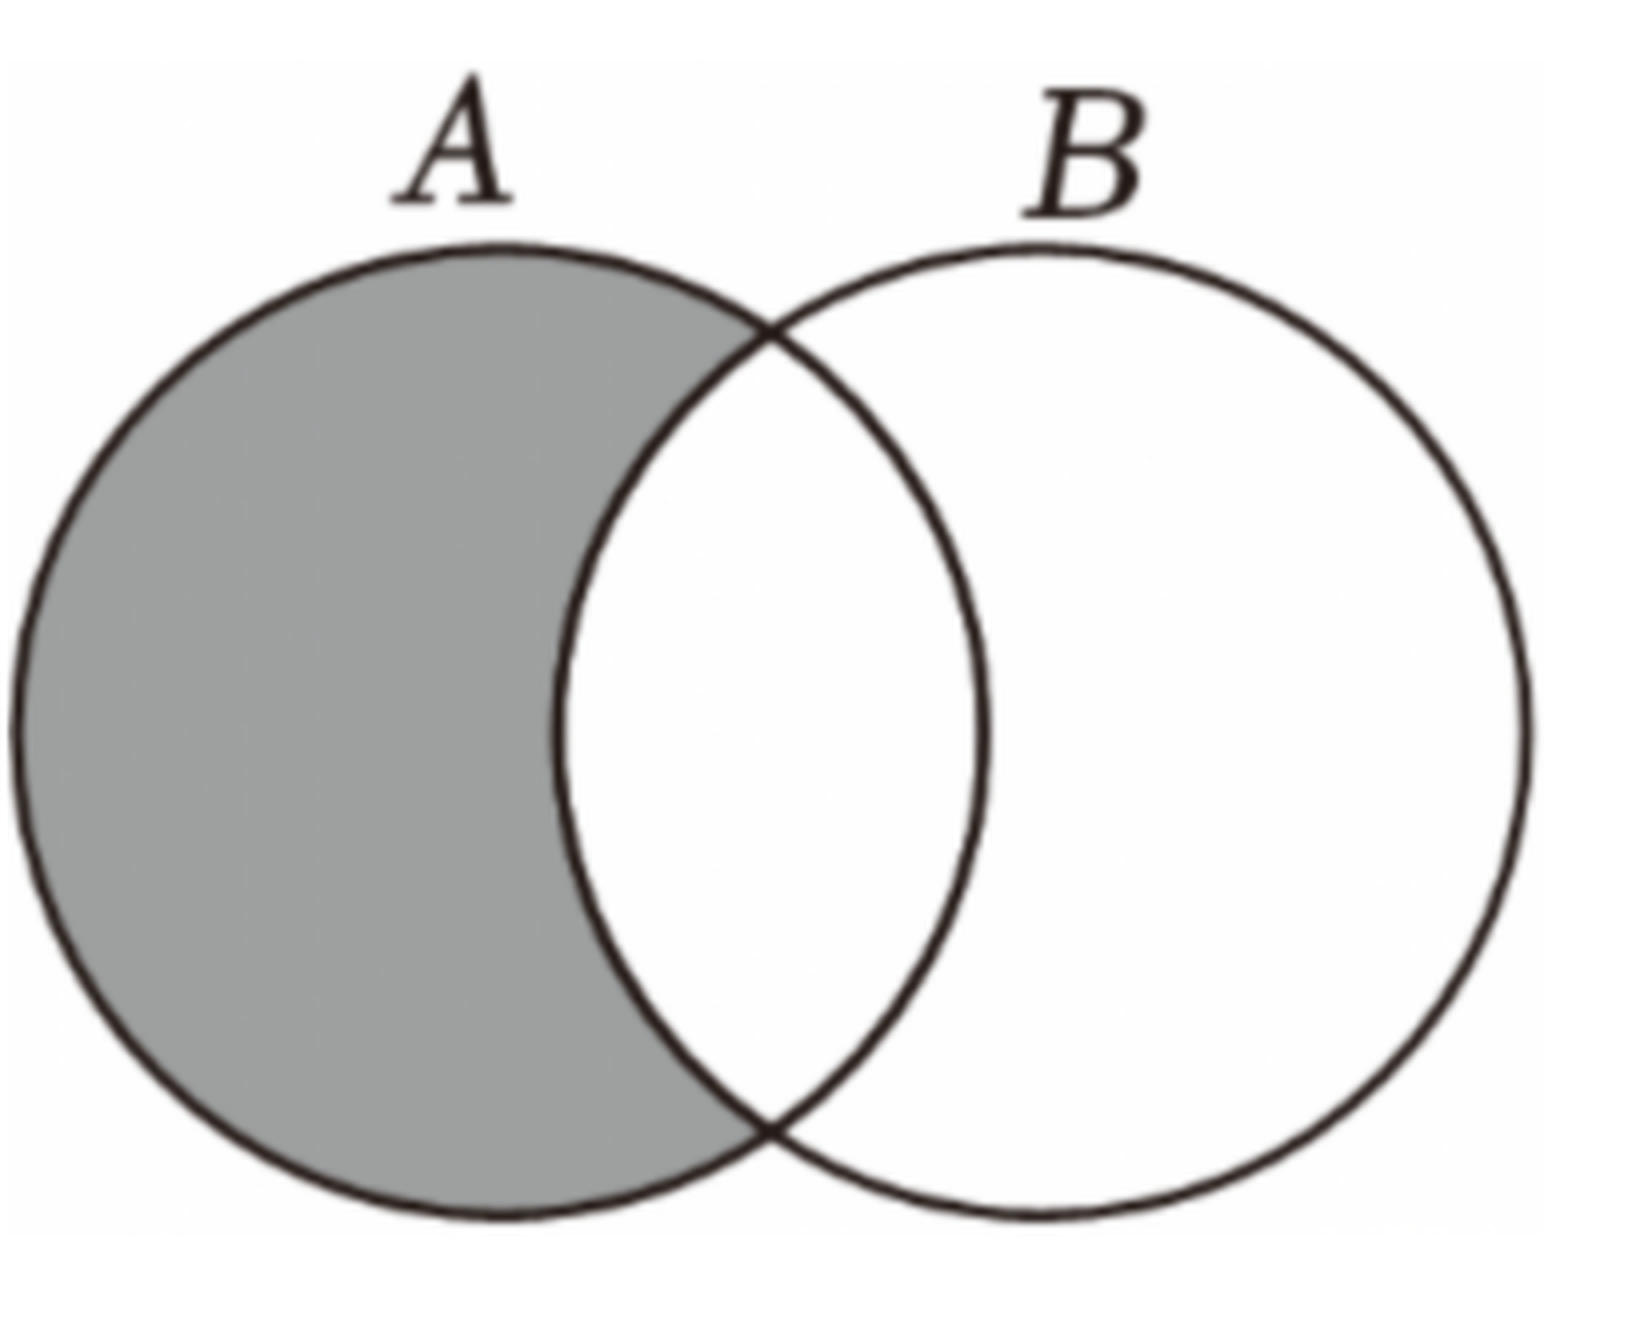
\includegraphics[width=0.30\textwidth]{figures/venn_A_minus_B_h38.png}
\end{center}

\ans{$\{1\}$}

\item 集合 $\{2,3,4,\cdots,2024,2025\}$ 的真子集的个数为 \blankline[4.4em].

\ans{$2^{2024}-1$}

\ifanswer
\solbegin
\step{集合 $\{2,3,4,\cdots,2024,2025\}$ 的真子集的个数为 $2^{2024}-1$.}
\solend

\fi

\item 已知集合 $A$ 中的元素都是正整数，其中最小的是 $1$，最大值是 $100$，除 $1$ 以外，每一个元
素都等于 $A$ 中的两个数（可以相同）的和，则集合 $A$ 中至少含有 \blankline[4.4em] 个元素.

\ans{$9$}

\ifanswer
\solbegin
\step{设 $A$ 中的数从小到大排列为 $1,a_1,a_2,\cdots,a_k,100$，}
\step{则 $a_1=1+1=2$；$3\leqslant a_2\leqslant 4$；$4\leqslant a_3\leqslant 8$；$5\leqslant a_4\leqslant 16$；$6\leqslant a_5\leqslant 32$；$7\leqslant a_6\leqslant 64$；}
\step{于是 $A$ 至少有八个数；}
\step{假设 $A$ 恰好有八个元素，由于 $a_5+a_6\leqslant 96<100$；}
\step{故必须有 $100=a_6+a_6$，$a_6=50$，}
\step{又 $a_4+a_5\leqslant 48$，同理 $a_5=25$，}
\step{但此时 $a_3+a_4\leqslant 24$，$a_5=2a_4$，$a_4=12.5$ 矛盾，}
\step{故 $A$ 不可能恰好有八个元素，因此 $A$ 至少有九个元素.}
\step{其九个数可以为 $1$，$2$，$3$，$6$，$12$，$13$，$25$，$50$，$100$.}
\solend

\fi

\item 已知集合 $\{x_1,x_2,x_3,x_4,x_5,x_6\}=\{1,2,3,4,5,6\}$，将 $x_i$ 与 $x_j$（其中 $i\in\{1,2,3\}$，
$j\in\{4,5,6\}$）的乘积 $x_ix_j$ 放入如图的 $3\times3$ 方格中，则方格中全部数之和的最大值为 \blankline[4.4em].

% 原卷的 $3\times3$ 方格是表格式内容（三行三列的公式），本稿按 高一03 的成例用 tabular 排出。
\begin{center}
\begin{tabular}{|c|c|c|}
\hline
$x_1x_4$ & $x_1x_5$ & $x_1x_6$ \\
\hline
$x_2x_4$ & $x_2x_5$ & $x_2x_6$ \\
\hline
$x_3x_4$ & $x_3x_5$ & $x_3x_6$ \\
\hline
\end{tabular}
\end{center}

\ans{$110$}

\ifanswer
\solbegin
\step{由表格数据得所有数之和为}
\step{$S=x_1x_4+x_1x_5+x_1x_6+x_2x_4+x_2x_5+x_2x_6+x_3x_4+x_3x_5+x_3x_6$，}
\step{所以 $S=(x_1+x_2+x_3)(x_4+x_5+x_6)$，}
\step{因为集合 $\{x_1,x_2,x_3,x_4,x_5,x_6\}=\{1,2,3,4,5,6\}$，}
\step{所以 $x_1+x_2+x_3+x_4+x_5+x_6=1+2+3+4+5+6=21$，}
\step{设 $t=x_1+x_2+x_3$，则 $6\leqslant t\leqslant 15$，$t\in\N^*$，}
\step{$S=t(21-t)=-\left(t-\dfrac{21}{2}\right)^2+\dfrac{441}{4}$，}
\step{当 $t=10$ 或 $t=11$ 时，$S=t(21-t)$ 取最大值，最大值为 $110$，}
\step{此时 $\{x_1,x_2,x_3\}=\{1,4,5\}$，$t=10$，所以可取最大值 $110$.}
\solend

\fi

\item 若 $[x]$ 表示不大于 $x$ 的最大整数，方程 $x^2-8[x]+7=0$ 的解集为 \blankline[4.4em].

\ans{$\{1,\sqrt{33},\sqrt{41},7\}$}

\ifanswer
\solbegin
\step{由题意，$x\geqslant[x]=\dfrac{x^2+7}{8}>0$，得 $x^2-8x+7\leqslant 0$，解得 $1\leqslant x\leqslant 7$，}
\step{$[x]=1$，$x^2=1$，$x=1$；}
\step{$[x]=2$，$x^2=9$，$x=3$ 与 $[x]=2$ 矛盾；}
\step{$[x]=3$，$x^2=17$，$x=\sqrt{17}$，$[x]=4$ 与 $[x]=3$ 矛盾；}
\step{$[x]=4$，$x^2=25$，$x=5$ 与 $[x]=4$ 矛盾；}
\step{$[x]=5$，$x^2=33$，$x=\sqrt{33}$，$[x]=5$；}
\step{$[x]=6$，$x^2=41$，$x=\sqrt{41}$，$[x]=6$；}
\step{$[x]=7$，$x^2=49$，$x=7$；}
\step{综上，方程 $x^2-8[x]+7=0$ 的解集为 $\{1,\sqrt{33},\sqrt{41},7\}$.}
\solend

\fi

\end{enumerate}

\bigsec{二、选择题}

\begin{enumerate}
\setcounter{enumi}{10}

\item 已知集合 $A=\{a,a^2\}$，$B=\{1,3\}$，若 $1\in A$，则 $A\cup B$ 中所有元素之和为\mbox{（\quad）}

\keepwithprev
A. $2$\qquad B. $3$\qquad C. $4$\qquad D. $5$

\ans{$B$}

\ifanswer
\solbegin
\step{因为 $1\in A$，集合 $A=\{a,a^2\}$，所以 $a=1$ 或 $a^2=1$，}
\step{若 $a=1$，则 $a=a^2$，与元素的互异性矛盾；}
\step{若 $a^2=1$，则 $a=1$（舍）或 $a=-1$，故 $A=\{-1,1\}$，$B=\{1,3\}$，}
\step{故 $A\cup B=\{-1,1,3\}$，所以 $A\cup B$ 中所有元素之和为 $-1+1+3=3$. 故选 $B$.}
\solend

\fi

\item 对于实数 $a$、$b$、$c$，下列命题正确的是\mbox{（\quad）}

\keepwithprev
A. 若 $a>b$，则 $ac^2>bc^2$\qquad B. 若 $a>b$，则 $a^2>b^2$

C. 若 $a>b$，则 $a|a|>b|b|$\qquad D. 若 $a>b>c>0$，则 $\dfrac{b}{a-b}<\dfrac{c}{a-c}$

\ans{$C$}

\ifanswer
\solbegin
\step{对于 $A$，若 $a>b$，$c=0$，则 $ac^2=bc^2$，故 $A$ 错误；}
\step{对于 $B$，若 $a>b$，取 $a=-1$，$b=-2$，则 $a^2<b^2$，故 $B$ 错误；}
\step{对于 $C$，若 $a>b>0$ 时，$a|a|-b|b|=a^2-b^2>0$，}
\step{当 $a>0>b$ 时，$a|a|-b|b|=a^2+b^2>0$，}
\step{当 $0>a>b$ 时，$a|a|-b|b|=b^2-a^2=(b-a)(b+a)>0$，}
\step{综上，若 $a>b$，则 $a|a|>b|b|$，故 $C$ 正确；}
\step{对于 $D$，若 $a>b>c>0$，$\dfrac{b}{a-b}-\dfrac{c}{a-c}=\dfrac{ab-bc-ac+bc}{(a-b)(a-c)}=\dfrac{a(b-c)}{(a-b)(a-c)}>0$，}
\step{故 $D$ 错误.}
\step{故选 $C$.}
\solend

\fi

\item 对于正整数集合 $A=\{a_1,a_2,\cdots,a_n\}(n\in\N^*,\ n\geqslant 3)$，如果去掉其中任意一个元素
$a_i(i=1,2,\cdots,n)$ 之后，剩余的所有元素组成的集合都能分为两个交集为空集的集合，且这
两个集合的所有元素之和相等，就称集合 $A$ 为平衡集. 记 $M=a_1+a_2+\cdots+a_n$. 若集合 $A$
是平衡集，并且存在 $a_i$ 为奇数，则集合 $A$ 中元素个数 $n$ 的奇偶性\mbox{（\quad）}

\keepwithprev
A. 与 $M$ 相关，既可以是奇数，又可以是偶数

B. 与 $M$ 无关，既可以是奇数，又可以是偶数

C. 与 $M$ 无关，必为偶数

D. 与 $M$ 无关，必为奇数

\ans{$D$}

\ifanswer
\solbegin
\step{正整数集合 $A=\{a_1,a_2,\cdots,a_n\}(n\in\N^*,\ n\geqslant 3)$，}
\step{因为集合 $A$ 是平衡集，设去掉元素 $a_i(i=1,2,\cdots,n)$，}
\step{由题意得 $A=A_1\cup A_2\cup\{a_i\}$，其中 $A_1\cap A_2=\varnothing$，}
\step{设集合 $A_1$ 和 $A_2$ 中的元素之和均为 $m$，所以 $M=2m+a_i$，其中 $i=1,2,\cdots,n$，}
\step{所以 $M-a_i=2m$，所以 $M-a_i$ 为偶数，其中 $i=1,2,\cdots,n$，}
\step{所以 $a_i(i=1,2,\cdots,n)$ 的奇偶性相同；}
\step{因为存在 $a_i$ 为奇数，所以 $a_i(i=1,2,\cdots,n)$ 均为奇数，}
\step{由 $M-a_i=2m$ 得 $M$ 也为奇数，且 $M=a_1+a_2+\cdots+a_n$，}
\step{所以 $n$ 也为奇数，所以 $n$ 必为奇数. 故选 $D$.}
\solend

\fi

\item 对于集合 $M=\{a\mid a=x^2-y^2,\ x\in\Z,\ y\in\Z\}$，给出如下三个结论：其中正确结论的个数
是\mbox{（\quad）}

\keepwithprev
①如果 $P=\{b\mid b=2n+1,\ n\in\Z\}$，那么 $P\sub M$；

②如果 $c=4n+2$，$n\in\Z$，那么 $c\notin M$；

③如果 $a_1\in M$，$a_2\in M$，那么 $a_1a_2\in M$.

\keepwithprev
A. $1$\qquad B. $2$\qquad C. $3$\qquad D. $0$

\ans{$C$}

\ifanswer
\solbegin
\step{对于①，$b=2n+1$，$n\in\Z$，则恒有 $2n+1=(n+1)^2-n^2$，}
\step{所以 $2n+1\in M$，即 $P=\{b\mid b=2n+1,n\in\Z\}$，则 $P\sub M$，①正确；}
\step{对于②，$c=4n+2$，$n\in\Z$，}
\step{若 $4n+2\in M$，则存在 $x$、$y\in\Z$ 使得 $x^2-y^2=4n+2$，}
\step{所以 $4n+2=(x+y)(x-y)$，又 $x+y$ 和 $x-y$ 同奇或同偶，}
\step{若 $x+y$ 和 $x-y$ 都是奇数，则 $(x+y)(x-y)$ 为奇数，而 $4n+2$ 是偶数；}
\step{若 $x+y$ 和 $x-y$ 都是偶数，则 $(x+y)(x-y)$ 能被 $4$ 整除，而 $4n+2$ 不能被 $4$ 整除，}
\step{所以 $4n+2\notin M$，即 $c\notin M$，②正确；}
\step{对于③，$a_1\in M$，$a_2\in M$，可设 $a_1=x_1^2-y_1^2$，$a_2=x_2^2-y_2^2$，$x_i$、$y_i\in\Z$；}
\step{则 $a_1a_2=(x_1^2-y_1^2)(x_2^2-y_2^2)=(x_1x_2)^2+(y_1y_2)^2-(x_1y_2)^2-(x_2y_1)^2$}
\step{$=(x_1x_2+y_1y_2)^2-(x_1y_2+x_2y_1)^2\in M$，那么 $a_1a_2\in M$，③正确.}
\step{综上，正确的命题是①②③. 故选 $C$.}
\solend

\fi

\end{enumerate}

\bigsec{三、解答题}

\begin{enumerate}
\setcounter{enumi}{14}

\item 已知 $A=\{x\mid a\leqslant x\leqslant -a+3\}$，$B=\{x\mid x<-1\text{ 或 }x>5\}$.

\begin{enumerate}[label=(\arabic*)]

\item 若 $A\cap B=\varnothing$，求 $a$ 的取值范围；

\item 若 $A\cup B=\R$，求 $a$ 的取值范围.

\end{enumerate}

\ans{（1）$[-1,+\infty)$；（2）$(-\infty,-2]$}

\ifanswer
\solbegin
\stepm{(1)}{①当 $A=\varnothing$ 时，$A\cap B=\varnothing$，需满足 $a>-a+3$，解得 $a>\dfrac32$，}
\step{故 $a$ 的取值范围为 $\left(\dfrac32,+\infty\right)$.}
\step{②当 $A\neq\varnothing$ 时，要使 $A\cap B=\varnothing$，需满足
$\begin{cases}a\leqslant\dfrac32\\[4pt] -a+3\leqslant 5\\[4pt] a\geqslant -1\end{cases}$，解得 $-1\leqslant a\leqslant\dfrac32$.}
\step{综上所述，$a$ 的取值范围是 $[-1,+\infty)$.}
\stepm{(2)}{因为 $A\cup B=\R$，$A=\{x\mid a\leqslant x\leqslant -a+3\}$，$B=\{x\mid x<-1\text{ 或 }x>5\}$，}
\step{所以 $\begin{cases}-a+3\geqslant 5\\[4pt] a\leqslant -1\end{cases}$，解得 $a\leqslant -2$，故所求 $a$ 的取值范围为 $(-\infty,-2]$.}
\solend

\fi

\ansspace[6]

\item 已知集合 $A=\{x\mid mx^2+x-2=0\}$，$B=\{x\mid 2x^2-5x-12=0\}$.

\begin{enumerate}[label=(\arabic*)]

\item 若 $A$ 中有且仅有 $1$ 个元素，求实数 $m$ 的值；

\item 已知集合 $C=A\cup B$，若 $C$ 的真子集有且仅有 $3$ 个，求实数 $m$ 的取值范围.

\end{enumerate}

\ans{（1）$m=0$ 或 $m=-\dfrac18$；（2）$\left\{m\mid m\leqslant -\dfrac18\right\}$}

\ifanswer
\solbegin
\stepm{(1)}{若 $m=0$，方程化为 $x-2=0$，此时方程有且仅有一个根 $x=2$；}
\step{若 $m\neq 0$，则 $\Delta=1^2-4\times m\times(-2)=0$，即 $m=-\dfrac18$ 时，}
\step{方程有两个相等的实根，此时集合 $A$ 中有且仅有一个元素，}
\step{所以实数 $m$ 的值为 $m=0$ 或 $m=-\dfrac18$；}
\stepm{(2)}{$B=\{x\mid 2x^2-5x-12=0\}=\left\{-\dfrac32,4\right\}$，}
\step{因为 $C=A\cup B$，若 $C$ 的真子集有且仅有 $3$ 个，则 $C$ 中有两个元素，}
\step{所以 $A\sub B$，由（1）得 $m=0$ 时，$A=\{2\}$，不符合 $A\sub B$，}
\step{当 $m\neq 0$ 时，若 $\Delta=1^2-4\times m\times(-2)<0$，解得 $m<-\dfrac18$，}
\step{此时 $A=\varnothing$，符合 $A\sub B$，}
\step{若 $\Delta=1^2-4\times m\times(-2)=0$，解得 $m=-\dfrac18$，}
\step{此时方程 $mx^2+x-2=0$ 的根为 $x=4$，集合 $A=\{4\}$，符合 $A\sub B$，}
\step{若 $\Delta=1^2-4\times m\times(-2)>0$，由 $A\sub B$，得 $A=\left\{-\dfrac32,4\right\}$，}
\step{此时有 $-\dfrac32+4=-\dfrac1m$ 且 $-\dfrac32\times 4=-\dfrac2m$，无解，}
\step{综上所述，实数 $m$ 的取值范围为 $\left\{m\mid m\leqslant -\dfrac18\right\}$.}
\solend

\fi

\ansspace[6]

\item 设 $A$ 是非空实数集，且 $0\notin A$. 若对于任意的 $x$、$y\in A$，都有 $xy\in A$，则称集合 $A$ 具
有性质 $P_1$；若对于任意的 $x$、$y\in A$，都有 $\dfrac xy\in A$，则称集合 $A$ 具有性质 $P_2$.

\begin{enumerate}[label=(\arabic*)]

\item 写出一个恰含有两个元素且具有性质 $P_1$ 的集合 $A$，并说明理由；

\item 证明：“非空实数集 $A$ 具有性质 $P_1$”是“非空实数集 $A$ 具有性质 $P_2$”的必要非充分条
件.

\end{enumerate}

\ans{（1）$A=\{-1,1\}$，理由见解析；（2）见解析}

\ifanswer
\solbegin
% 注：原卷本题 (1) 的解析里“证明”一词重复出现两次（一次接在分号后、一次另起一行），
%     本稿照原卷重复录入，未去重。
\stepm{(1)}{$A=\{-1,1\}$，证明：恰含有两个元素且具有性质 $P_1$ 的集合 $A=\{-1,1\}$；}
\step{证明：$1\times 1=1\in A$，$1\times(-1)=-1\in A$，$-1\times 1=-1\in A$，$-1\times(-1)=1\in A$；}
\stepm{(2)}{若集合 $A$ 具有性质 $P_2$，不妨设 $a\in A$，}
\step{由非空数集 $A$ 具有性质 $P_2$，有 $\dfrac aa=1\in A$.}
\step{①$A=\{1\}$，易得此时集合 $A$ 具有性质 $P_1$.}
\step{②数集 $A$ 只含有两个元素，不妨设 $A=\{1,a_1\}$，}
\step{由 $\dfrac{1}{a_1}=a_1$，且 $a_1\neq 1$，解得 $a_1=-1$，此时集合 $A$ 具有性质 $P_1$.}
\step{③实数集 $A$ 含有两个以上的元素，不妨设不为 $1$ 的元素 $a_1$、$a_2\in A$，}
\step{则有 $\dfrac{1}{a_1}\in A$，由于集合 $A$ 具有性质 $P_2$，}
\step{所以有 $a_2\div\dfrac{1}{a_1}=a_1a_2\in A$，这说明集合 $A$ 具有性质 $P_1$.}
\step{综上，若非空实数集 $A$ 具有性质 $P_2$，则集合 $A$ 具有性质 $P_1$，}
\step{所以“非空实数集 $A$ 具有性质 $P_1$”是“非空实数集 $A$ 具有性质 $P_2$”的}
\step{必要条件.}
\step{取正偶数集 $A=\{x\mid x=2n,\ n\in\N^*\}$，}
\step{对任意的 $2m$、$2n\in A$，$m$、$n\in\N^*$，}
\step{有 $2m\times 2n=4mn\in A$，故 $A$ 具有性质 $P_1$，}
\step{取 $x=2$，$y=4$，则 $\dfrac xy=\dfrac12\notin A$，故 $A$ 不具有性质 $P_2$，}
\step{所以“非空实数集 $A$ 具有性质 $P_1$”不是“非空实数集 $A$ 具有性质 $P_2$”的}
\step{充分条件.}
\step{综上，“非空实数集 $A$ 具有性质 $P_1$”是“非空实数集 $A$ 具有性质 $P_2$”的}
\step{必要非充分条件.}
\solend

\fi

\ansspace[8]

\item 已知命题 $p$：关于 $x$ 的方程 $x^2+mx+1=0$ 有两个不同的正根；命题 $q$：关于 $x$ 的方程
$4x^2+4(m-2)x=-1$ 有实根.

\begin{enumerate}[label=(\arabic*)]

\item 若命题 $q$ 为假命题，求整数 $m$ 的解集；

\item 若命题 $p$ 为真命题，且关于 $x$ 的方程 $x^2+mx+1=0$ 的两个实数根 $x_1$、$x_2$ 满足
$3x_1+2x_2=5$，求实数 $m$ 的取值集合；

\item 若命题 $p$ 和命题 $q$ 有且仅有一个成立，求实数 $m$ 的取值范围.

\end{enumerate}

\ans{（1）$\{2\}$；（2）$\left\{-\dfrac{13}{6}\right\}$；（3）$[-2,1]\cup[3,+\infty)$}

\ifanswer
\solbegin
\stepm{(1)}{命题 $q$：关于 $x$ 的方程 $4x^2+4(m-2)x=-1$ 有实根为假命题，}
\step{即 $4x^2+4(m-2)x+1=0$ 无实根，}
\step{则 $\Delta=16(m-2)^2-16<0$，则 $1<m<3$，则整数 $m$ 的解集为 $\{2\}$；}
\stepm{(2)}{若命题 $p$ 为真命题，且关于 $x$ 的方程 $x^2+mx+1=0$ 的两个实数根 $x_1$、$x_2$，}
\step{满足 $3x_1+2x_2=5$，则方程 $x^2+mx+1=0$ 有两个不同的正根，}
\step{则 $\begin{cases}\Delta=m^2-4>0\\[4pt] x_1+x_2=-m>0\end{cases}$，则 $m<-2$，}
\step{又 $\begin{cases}x_1+x_2=-m\\[4pt] x_1x_2=1\\[4pt] 3x_1+2x_2=5\end{cases}$，
则 $\begin{cases}x_1=5+2m\\[4pt] x_2=-3m-5\end{cases}$，则 $(5+2m)(-3m-5)=1$，}
\step{得 $m=-2$ 或 $m=-\dfrac{13}{6}$，又因为 $m<-2$，所以 $m=-\dfrac{13}{6}$，}
\step{所以实数 $m$ 的取值集合为 $\left\{-\dfrac{13}{6}\right\}$；}
\stepm{(3)}{由（2）得当 $p$ 为真时，则有 $m<-2$，}
\step{当 $q$ 为真时，$\Delta=16(m-2)^2-16\geqslant 0$，解得 $m\leqslant 1$ 或 $m\geqslant 3$，}
\step{又因为命题 $p$ 和命题 $q$ 只有一个为真，所以
$\begin{cases}m<-2\\[4pt] 1<m<3\end{cases}$ 或 $\begin{cases}m\geqslant -2\\[4pt] m\leqslant 1\text{ 或 }m\geqslant 3\end{cases}$，}
\step{解得 $-2\leqslant m\leqslant 1$ 或 $m\geqslant 3$，所以实数 $m$ 的取值范围为 $[-2,1]\cup[3,+\infty)$.}
\solend

\fi

\ansspace[8]

% 注：原卷此处作“设 $n\in\N^*$，集合含有 $3n$ 个元素”，**漏了符号 $U$**（应作“集合 $U$
%     含有 $3n$ 个元素”）——$U$ 直到本句末尾“则称 $U$ 为三分集合”才出现、此前无定义。
%     本稿照录未补，见文件头“原卷笔误/存疑”⑦。
\item 设 $n\in\N^*$，集合含有 $3n$ 个元素，若存在三个 $n$ 元集合 $A$、$B$、$C$ 满足如下两个条件，
则称 $U$ 为三分集合.

①$U=A\cup B\cup C$；

②$A$、$B$、$C$ 元素可分别排列为有序数组 $(a_1,a_2,\cdots,a_n)$，$(b_1,b_2,\cdots,b_n)$ 及
$(c_1,c_2,\cdots,c_n)$，使得对 $\forall i=1,2,\cdots,n$，均有 $a_i+b_i=c_i$.

特别地，当 $U=\{1,2,3,4,\cdots,3n-2,3n-1,3n\}$ 为三分集合时，称 $n$ 为完美三分数.

如：因为 $U=\{1,2,3\}$ 为三分集合，所以 $n=1$ 为最小完美三分数.

\begin{enumerate}[label=(\arabic*)]

\item 请判断下列两个集合是否为三分集合（直接写出结论）：

$U_1=\{1,2,3,4,5,6\}$，$U_2=\{1,3,5,7,8,9,10,11,12\}$；

\item 求出大于 $1$ 的最小完美三分数；

\item 请判断是否存在无穷多个完美三分数？若存在，请说明理由；若不存在，则求出最大的
完美三分数.

\end{enumerate}

\ans{（1）$U_1$ 不是三分集合，$U_2$ 是三分集合；（2）$4$；（3）存在，理由见解析}

\ifanswer
\solbegin
\stepm{(1)}{(i)$U_1=\{1,2,3,4,5,6\}$ 不是三分集合，下面用反证法证明：}
\step{证明：假设 $U=\{1,2,3,4,5,6\}$ 是三分集合，}
\step{设 $A=\{a_1,a_2\}$，$B=\{b_1,b_2\}$，$C=\{c_1,c_2\}$，不妨设 $c_1<c_2$，}
\step{因为 $a_1+b_1=c_1$，$a_2+b_2=c_2$，}
\step{所以 $a_1+b_1+a_2+b_2+c_1+c_2=2(c_1+c_2)=1+2+3+4+5+6=21$，}
% 注：原卷此步印“所以 $c_1+c_2=2$”，与上一行的 $2(c_1+c_2)=21$ **不自洽**
%     （应作 $\dfrac{21}2$）；同题 $n=3$ 处的同型推理原卷写的是 $\dfrac{45}2$，故此处是原卷笔误。
%     本稿照录未改，见文件头“原卷笔误/存疑”⑧。
\step{所以 $c_1+c_2=2$，这与 $c_1,c_2\in\N^*$ 矛盾，故假设错误，}
\step{故 $U_1=\{1,2,3,4,5,6\}$ 不是三分集合；}
\step{(ii)$U_2=\{1,3,5,7,8,9,10,11,12\}$ 是三分集合，理由如下：}
\step{令 $A=\{1,3,5\}$，$B=\{9,8,7\}$，$C=\{10,11,12\}$，}
\step{则 $A\cup B\cup C=U=\{1,3,5,7,8,9,10,11,12\}$，满足条件①；}
\step{又 $1+9=10$；$3+8=11$；$5+7=12$，所以满足条件②，}
\step{所以 $U_2=\{1,3,5,7,8,9,10,11,12\}$ 是三分集合；}
\stepm{(2)}{由（1）得，当 $n=2$ 时，$U=\{1,2,3,4,5,6\}$ 不是三分集合；}
\step{当 $n=3$ 时，$U=\{1,2,3,4,5,6,7,8,9\}$，}
\step{假设 $U=\{1,2,3,4,5,6,7,8,9\}$ 是三分集合，}
\step{同理由 $a_1+b_1+a_2+b_2+a_3+b_3+c_1+c_2+c_3$}
\step{$=2(c_1+c_2+c_3)=1+2+\cdots+9=45$，$c_1+c_2+c_3=\dfrac{45}{2}$，}
\step{可推出与 $c_1$、$c_2$、$c_3\in\N^*$ 矛盾，故假设也错误，}
\step{所以 $U=\{1,2,3,4,5,6,7,8,9\}$ 不是三分集合；}
\step{当 $n=4$ 时，$U=\{1,2,3,\cdots,12\}$，}
\step{存在三个 $4$ 元集合 $A=\{1,2,4,3\}$，$B=\{5,8,7,9\}$，$C=\{6,10,11,12\}$，}
\step{满足 $U=\{1,2,3,\cdots,12\}$ 为三分集合的两个条件，}
\step{故大于 $1$ 的最小完美三分数为 $4$；}
\stepm{(3)}{存在无穷多个完美三分数，理由如下：}
\step{由题意得，$n=1$ 为最小完美三分数，}
\step{当 $n=5$ 时，$U=\{1,2,3,\cdots,15\}$，}
\step{存在三个 $5$ 元集合 $A=\{1,3,5,7,2\}$，$B=\{11,10,9,8,4\}$，$C=\{12,13,14,15,6\}$，}
\step{满足三分集合的条件，故 $5$ 为完美三分数；}
\step{当 $n=21$ 时，$U=\{1,2,3,\cdots,63\}$，}
\step{存在如下三个 $21$ 元的集合满足三分集合的条件：}
\step{$A=\{1,3,5,7,\cdots,29,31,2,6,10,14,4\}$，}
\step{$B=\{47,46,45,44,\cdots,33,32,22,20,18,16,8\}$，}
\step{$C=\{48,49,50,51,\cdots,62,63,24,26,28,30,12\}$，}
\step{故 $21$ 为完美三分数.}
\step{首先证明：若 $n=k$，$k\in\N^*$ 为三分完美数，}
\step{则 $n=4k+1$，$k\in\N^*$ 也为三分完美数，}
% 注：下一行原卷印作“$U_{k+1}=U_{k+1}=\{2,3,\cdots,12k+3\}$”——等号两边记号相同，
%     依上下文疑当作 $U'_{k+1}=U_{4k+1}$，且此处集合自 2 起（前文 $U_{4k+1}$ 自 1 起）；
%     本稿照录原卷，未代为改写。
\step{证明：记 $U_k=\{1,2,3,\cdots,3k\}$，$U_{4k+1}=\{1,2,3,\cdots,12k+3\}$，}
\step{若 $n=k$，$k\in\N^*$ 为三分完美数，则 $U_k$ 为三分集合，}
\step{即存在三个 $k$ 元集合 $A$、$B$、$C$ 满足如下两个条件，}
\step{①$U_k=A\cup B\cup C$；}
\step{②$A$、$B$、$C$ 元素可分别排列为有序数组 $(a_1,a_2,\cdots,a_k)$，}
\step{$(b_1,b_2,\cdots,b_k)$ 及 $(c_1,c_2,\cdots,c_k)$，}
\step{使得对 $\forall i=1,2,3,\cdots,k$，均有 $a_i+b_i=c_i$，}
\step{则可得到对 $\forall i=1,2,3,\cdots,k$，$2a_i+2b_i=2c_i$，}
\step{故集合 $\{2,4,6,\cdots,6k\}$ 也满足三分集合的两个条件，其也为三分集合，}
\step{下面记集合 $\{2,4,6,\cdots,6k\}=2U_k$，}
\step{对 $n=4k+1$，集合 $U_{k+1}=U_{k+1}=\{2,3,\cdots,12k+3\}=(2U_k)\cup\complement_{U_{4k+1}}(2U_k)$，}
\step{构造集合 $A'=\{1,3,5,7,\cdots,6k+1\}$，共有 $3k+1$ 个奇数；}
% 注：下一行原卷印作“$B'=\{6k+3k+2,6k+3k+1,6k+3k,6k+3k-1,\cdots,6k+2\}$”，
%     按与后文 $C'$ 相接，前四项当写作 $9k+2$、$9k+1$、$9k$、$9k-1$；本稿照录原卷。
\step{集合 $B'=\{6k+3k+2,6k+3k+1,6k+3k,6k+3k-1,\cdots,6k+2\}$，}
\step{共有 $3k+1$ 个逐个减小的连续正整数；}
\step{集合 $C'=\{9k+3,9k+4,9k+5,9k+6,\cdots,12k+3\}$，}
\step{共有 $3k+1$ 个逐个增大的连续正整数；}
\step{得这三个 $3k+1$ 元集合 $A'$、$B'$、$C'$ 满足如下两个条件，}
\step{①集合 $A'\cup B'\cup C'=\complement_{U_{4k+1}}(2U_k)$；}
\step{②$A'$、$B'$、$C'$ 元素可分别排列为有序数组 $(a_1,a_2,\cdots,a_{3k+1})$，}
\step{$(b_1,b_2,\cdots,b_{3k+1})$ 及 $(c_1,c_2,\cdots,c_{3k+1})$，}
\step{使得对 $\forall i=1,2,3,\cdots,3k+1$，均有 $a_i+b_i=c_i$；}
\step{故 $\complement_{U_{4k+1}}(2U_k)$ 为三分集合，而已知 $U_k$ 为三分集合，}
\step{将其对应与 $A'$、$B'$、$C'$ 合并，}
% 注：原卷此处印“令 $A''=A\cup A'$”（$B''$、$C''$ 同）。按同段上文“记集合
%     $\{2,4,6,\cdots,6k\}=2U_k$”，此处疑当作 $A''=2A\cup A'$——否则
%     $A''\cup B''\cup C''=U_k\cup\complement_{U_{4k+1}}(2U_k)\neq U_{4k+1}$，与本段结论冲突。
%     本稿照录未改，见文件头“原卷笔误/存疑”⑨。
\step{令 $A''=A\cup A'$，$B''=B\cup B'$，$C''=C\cup C'$，}
\step{则这三个 $4k+1$ 元集合 $A''$、$B''$、$C''$，}
\step{满足 $A''\cup B''\cup C''=U_{4k+1}$，且满足条件②，}
\step{故 $U_{4k+1}=\{1,2,3,\cdots,12k+3\}$ 为三分集合，}
\step{因此可得，若 $n=k$ 为三分完美数，则 $n=4k+1$ 也为三分完美数，}
\step{由 $1$，$5$，$21$ 为完美三分数，结合所证结论得，存在无穷多个完美三分数.}
\solend

\fi

\ansspace*[12]

\end{enumerate}

\end{document}
"
%
% 原始材料是微信公众号图文（公众号“魔都数学加油站”连载“27学年高一 38”，署名“破晓”，
% 2026-09-26 21:29 发布，原文标题“27学年高一38——2026-2027年上海市大同中学高一上周末作业3”，
% 原文链接 https://mp.weixin.qq.com/s/O_O60vCIiGi2xponAo4irw ），正文为 12 张 PNG 页。
% **同一篇里各页分辨率不一致**（2560×3620 与 4762×6735 两档混排：第 1、10、11、12 页为
% 2560×3620，第 2—9 页为 4762×6735）。原文本身就是一份**讲评版**——有的题下方只印
% 【答案】行，有的只印【解析】。试题文字、答案与解析均照原卷录入，未改内容。卷面的粉色
% 斜水印“魔都数学加油站”属水印，未录入。
%
% 本卷共 **17 题**：填空题 8 题（第 3—10 题）、选择题 4 题（第 11—14 题）、解答题 5 题
% （第 15—19 题）；插图 1 张（第 6 题 Venn 图）。三版页数：试卷版 4 页 / 答案版 11 页 /
% 紧凑版 3 页，`Overfull`／`Underfull`／`Missing character` 告警均为 0。
%
% 卷首标题：原卷印作“2026-2027 年大同中学高一上周末作业 3”（公众号原文标题里的“上海市”
% 三字卷面标题行没有，本稿照卷面），年份区间按全稿惯例排 en dash，前缀照原卷保留“年”。
%
% 与原卷的排版差异（均已在 README“说明”中交代）：
%   ① 原文自**第 3 题**起（第 1、2 题未在该文中发布），故本稿题号亦自 3 起，填空题以
%      \setcounter{enumi}{2} 起编；选择、解答两节各按上一节末号另设 \setcounter
%      （选择题 \setcounter{enumi}{10}、解答题 \setcounter{enumi}{14}）；
%   ② 原卷本就印有“一、填空题”“二、选择题”“三、解答题”三节标题，本稿照原卷分节，
%      只把标题改排成全稿统一的“大节标题”样式；
%   ③ 原卷是“讲评版”：第 3、6 题只印【答案】行，第 4、5、7、8、9、10 题与第 11—19 题印
%      【解析】；本稿统一改为试卷版隐去、答案版以 \ans{}／\ifanswer 块给出，两版彻底分离。
%      其中第 4、5、7、8、9、10 题与第 11—14 题的答案，原卷写在【解析】末句，本稿另提为
%      \ans{}；第 15—19 题原卷只有【解析】、无独立答案行，本稿亦补了摘要式 \ans{}。
%      **故本卷 17 题每题都有 \ans**——比“只印【解析】的填空、解答题不另提 \ans”的
%      高一31／高一34 更彻底，与 高一21 第 11 题（填空，答案在【解析】末句，本稿另提）同类；
%      （本仓对“另提 \ans{}”的做法各卷不一，见 README 对应专记的核对面。）
%   ④ 数集记号原卷两套并用：第 3、5 题的实数集作粗体 $\mathbf{R}$，第 8、14、17、18 题等的
%      整数集、自然数集作斜体 $Z$、$N$，本稿按全稿惯例统一写作 $\R$、$\Z$、$\N$；
%   ⑤ 原卷填空的横线宽度不一（约 1.8—3.6 字宽），本稿按全稿惯例统一排 \blankline[4.4em]；
%   ⑥ 中文括注原卷用半角“(  )”，本稿按全稿惯例排全角；选择题的作答括注统一排
%      \mbox{（\quad）}（第 14 题的作答括注原卷印在 ①②③ 三个命题**之前**，本稿照原卷次序）；
%      数学式内部的括注（如第 4 题的 $p\%(0<p<100)$、第 13 题的 $a_i(i=1,2,\cdots,n)$）照原样
%      留在行内公式里，未改全角；
%   ⑦ 原卷并列的字母（“x,y”“a,b,c”）不加标点或作半角逗号，本稿按全稿惯例改排顿号；
%   ⑧ 第 6 题的 Venn 图取原卷截图、4× LANCZOS 放大（figures/venn_A_minus_B_h38.png，
%      见该处 \includegraphics 前的注释）；第 9 题的 $3\times3$ 方格属**表格式**内容，
%      本稿按 高一03 的成例用 tabular 排出，未截图；
%   ⑨ 原卷未印副标题，本稿按**本卷实际内容**补出副标题“集合与常用逻辑用语”（依据见下条）；
%   ⑩ 原卷【解析】**一个印刷行照录为一条 `\step`**（原卷的折行也照录为独立一条，如第 17 题
%      末三处“…的”／“必要条件.”这类跨行句、第 9 题“由表格数据得所有数之和为”／
%      “$S=\cdots$，”），使答案版的排布与原卷讲评版逐行对应；全卷 15 处【解析】合计
%      **191 条 `\step` ＝ 原卷 191 行**（逐处：5、5、1、9、9、9、4、9、9、12、6、14、21、13、65）。
%
% 副标题（\examtitlest 第二个参数）：本卷卷面未印副标题，由本稿补出，取值按 2026-09-26 起的
%   新口径“只用本卷实际内容的模块名”定为“集合与常用逻辑用语”。依据：全卷 17 题
%   （第 3—19 题）中，第 3、5、6、7、8、9、10、11、13、14、15、16、17、18、19 题共 15 题
%   是集合的运算与关系、子集计数、集合新定义（性质 $P_1$／$P_2$、平衡集、三分集合），以及
%   命题与逻辑（第 3 题即用反证法证明“$x+y>2\Rightarrow x>1$ 或 $y>1$”这一命题）；不等式只
%   出现在第 4 题（降价提价的应用比较）、第 12 题（不等式命题真假）与第 10 题解析里解一元
%   二次不等式，合计不足全卷的三分之一，故不并标“不等式”。
%
% 原卷笔误/存疑（均照抄原卷、未改，见源码中该处上方注释）：
%   ① 第 19 题 (3) 的证明里印作“集合 $U_{k+1}=U_{k+1}=\{2,3,\cdots,12k+3\}$”——等号两边
%      记号相同（依上下文疑当作 $U'_{k+1}=U_{4k+1}$），且此处集合自 $2$ 起，而前文
%      $U_{4k+1}=\{1,2,3,\cdots,12k+3\}$ 自 $1$ 起；本稿照录；
%   ② 第 19 题 (3) 的证明里印作
%      “$B'=\{6k+3k+2,6k+3k+1,6k+3k,6k+3k-1,\cdots,6k+2\}$”——按与后文
%      $C'=\{9k+3,9k+4,9k+5,9k+6,\cdots,12k+3\}$ 相接，前四项当写作 $9k+2$、$9k+1$、
%      $9k$、$9k-1$（即 $6k+3k+2$ 等），原卷即作“$6k+3k+\cdots$”形式，本稿照录；
%   ③ 第 19 题的术语前后不一：题干与 (1)(2)(3) 用“完美三分数”，而 (3) 的证明里五次写作
%      “三分完美数”（词序不同）；本稿五处都照录；
%   ④ 第 14 题题干作“给出如下三个结论：其中正确结论的个数是（\quad）”，此处冒号疑当作
%      逗号，本稿照录；
%   ⑤ 第 17 题题干作“非空实数集”，其解析有一处写作“非空数集”；本稿照录；
%   ⑥ 第 17 题 (1) 的【解析】原卷连写“…集合 $A=\{-1,1\}$；证明：…；证明：…”，“证明”
%      一词重复出现两次（第一次在分行处、第二次另起一行），本稿照原卷重复录入，未去重。
%   ⑦ 第 19 题**题干漏字**：原卷作“19.设 $n\in\N^*$，集合含有 $3n$ 个元素…则称 $U$ 为
%      三分集合”——首句漏了符号 $U$（应作“集合 $U$ 含有 $3n$ 个元素”），$U$ 直到结论句
%      才出现、此前无定义；本稿照录未补（见该处上方注释）。
%   ⑧ 第 19(1)(i) 的【解析】**自相矛盾**：上一行印“$a_1+b_1+a_2+b_2+c_1+c_2=2(c_1+c_2)
%      =1+2+3+4+5+6=21$”，下一行却印“所以 $c_1+c_2=2$”（由 $2(c_1+c_2)=21$ 应得
%      $c_1+c_2=\dfrac{21}2$，非整数、才与 $c_1,c_2\in\N^*$ 矛盾）；同题 $n=3$ 处的同型
%      推理原卷就写对了（$\dfrac{45}2$），故此处是原卷笔误；本稿照录未改（见该处上方注释）。
%   ⑨ 第 19(3) 的【解析】印“令 $A''=A\cup A'$，$B''=B\cup B'$，$C''=C\cup C'$”——按同段
%      上文“记集合 $\{2,4,6,\cdots,6k\}=2U_k$”，$A''$ 等疑当作 $2A\cup A'$（$B''$、$C''$ 同），
%      否则 $A''\cup B''\cup C''=U_k\cup\complement_{U_{4k+1}}(2U_k)\neq U_{4k+1}$；本稿照录未改
%      （见该处上方注释）。

\documentclass[a4paper,11pt]{article}
\usepackage{common}

\begin{document}

\examtitlest[3]{2026--2027 年大同中学高一上周末作业 3}{集合与常用逻辑用语}

\bigsec{一、填空题}

\begin{enumerate}
% 原卷填空题自第 3 题起（第 1、2 题未在该文中发布），须与选择、解答两节的 \setcounter 对齐
\setcounter{enumi}{2}

\item 设 $x$、$y\in\R$，若 $x+y>2$，则 $x>1$ 或 $y>1$ 是真命题. 这个命题可以用反证法去证明，
可以假设：\blankline[4.4em].

\ans{$x\leqslant 1$ 且 $y\leqslant 1$}

\item 已知某商品的原价为 $a$ 元，由于市场原因，先降价 $p\%(0<p<100)$ 出售，一段时间后，
再提价 $p\%$ 出售，则该商品提价后的售价 \blankline[4.4em] 该商品的原价（填“高于”“低于”或“等于”）.

\ans{低于}

\ifanswer
\solbegin
\step{由题意得第一次降价后的售价为 $a(1-p\%)$ 元，}
\step{第二次提价后的售价为 $a(1-p\%)(1+p\%)$ 元，}
\step{因为 $0<p<100$，所以 $0<p\%<1$，}
\step{因为 $a(1-p\%)(1+p\%)=a[1-(p\%)^2]<a$，}
\step{即该商品提价后的售价低于该商品的原价.}
\solend

\fi

\item 若集合 $A=\{x\mid ax^2+ax+1=0,\ a\in\R,\ x\in\R\}$ 的子集只有两个，则实数 $a=$ \blankline[4.4em].

\ans{$4$}

\ifanswer
\solbegin
\step{集合 $A=\{x\mid ax^2+ax+1=0\}$ 的子集只有两个，}
\step{所以 $A$ 有且只有一个元素，}
\step{①若 $a=0$，则 $A=\varnothing$ 不成立；}
\step{②若 $a\neq 0$，则 $\Delta=a^2-4a=0$，解得 $a=4$（$0$ 舍）.}
\step{故 $a=4$.}
\solend

\fi

\item 如图，已知集合 $A=\{1,2,3,4,5\}$，集合 $B=\{2,3,4,5,9\}$，则图中阴影部分所表示的
集合为 \blankline[4.4em].

% 图取原卷截图（01.png，2560×3620）右栏，4× LANCZOS 放大；为避免与 高一11 的
% figures/venn_A_minus_B.png 同名，按 高一32 的成例加 _h38 后缀。
\begin{center}
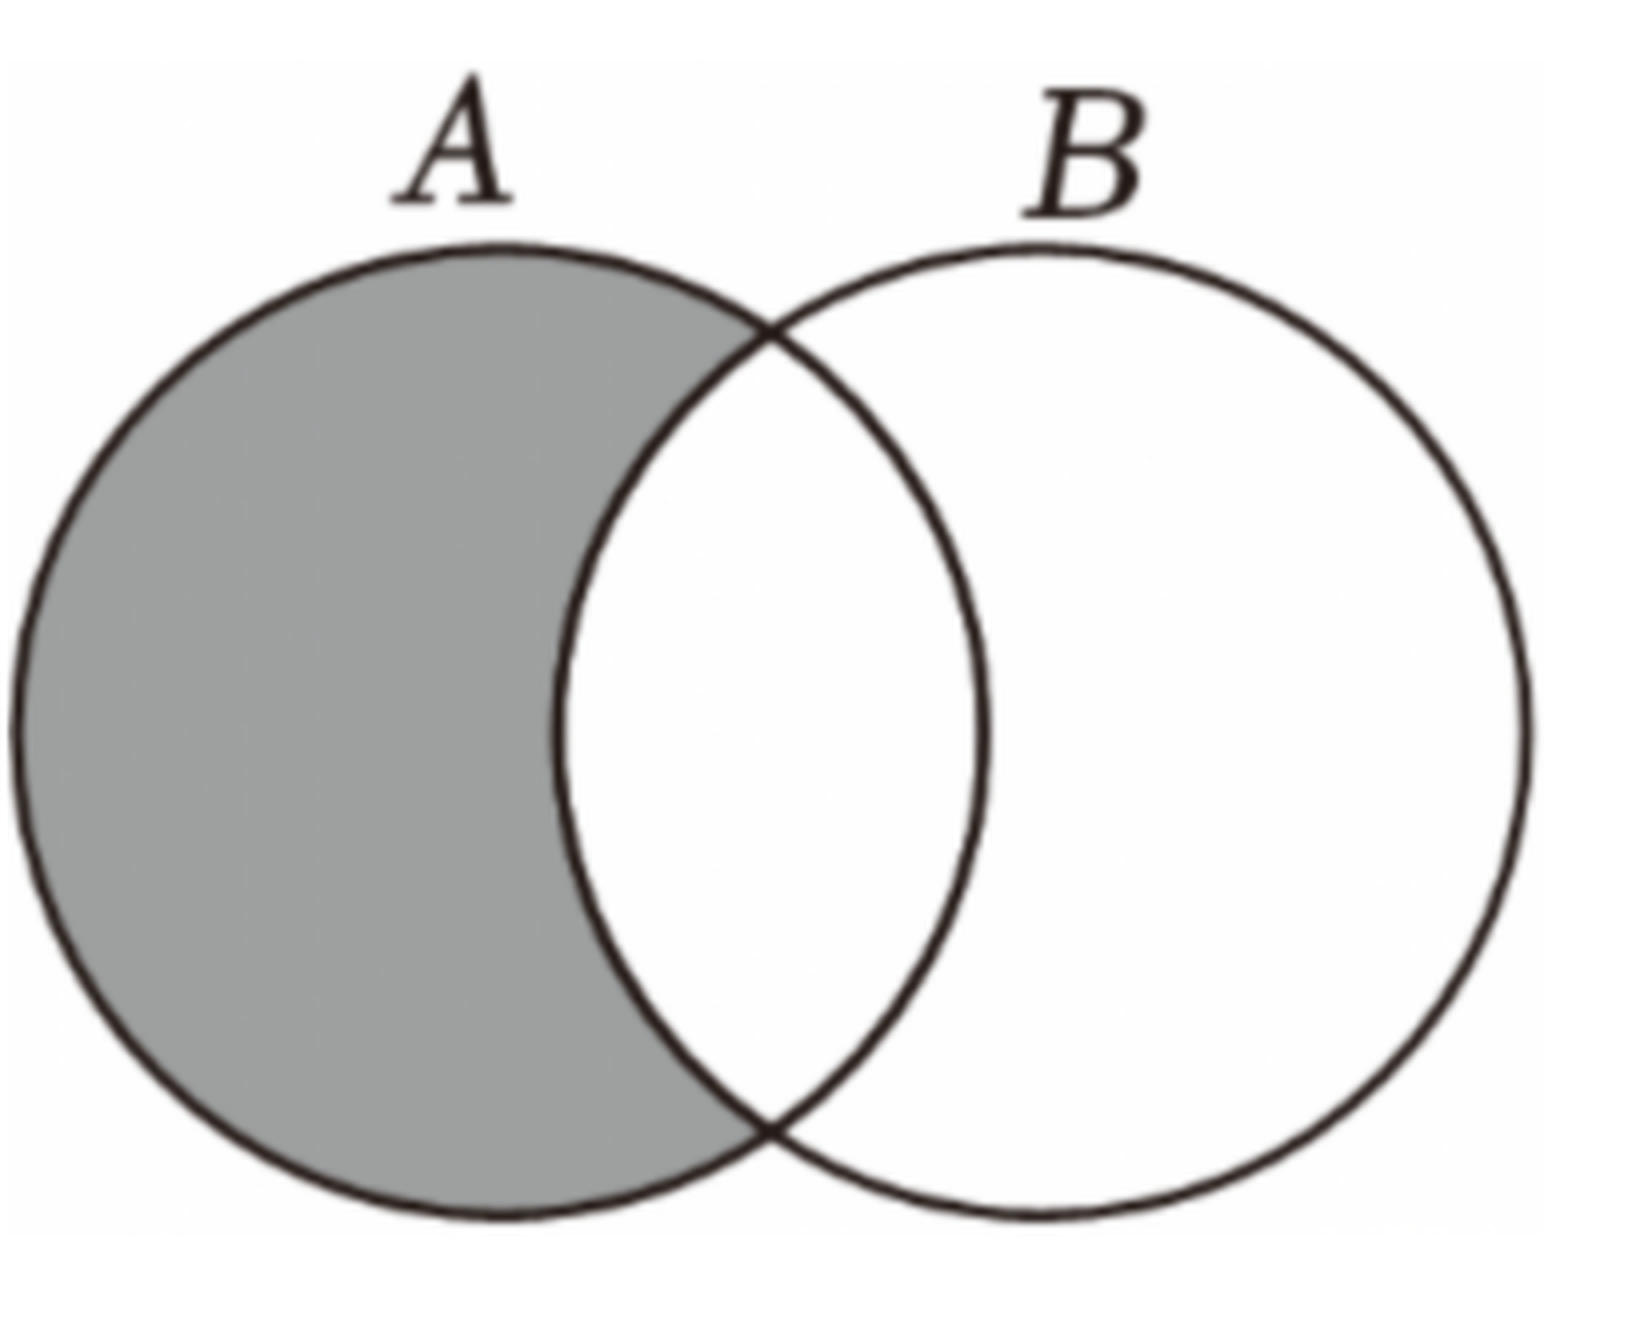
\includegraphics[width=0.30\textwidth]{figures/venn_A_minus_B_h38.png}
\end{center}

\ans{$\{1\}$}

\item 集合 $\{2,3,4,\cdots,2024,2025\}$ 的真子集的个数为 \blankline[4.4em].

\ans{$2^{2024}-1$}

\ifanswer
\solbegin
\step{集合 $\{2,3,4,\cdots,2024,2025\}$ 的真子集的个数为 $2^{2024}-1$.}
\solend

\fi

\item 已知集合 $A$ 中的元素都是正整数，其中最小的是 $1$，最大值是 $100$，除 $1$ 以外，每一个元
素都等于 $A$ 中的两个数（可以相同）的和，则集合 $A$ 中至少含有 \blankline[4.4em] 个元素.

\ans{$9$}

\ifanswer
\solbegin
\step{设 $A$ 中的数从小到大排列为 $1,a_1,a_2,\cdots,a_k,100$，}
\step{则 $a_1=1+1=2$；$3\leqslant a_2\leqslant 4$；$4\leqslant a_3\leqslant 8$；$5\leqslant a_4\leqslant 16$；$6\leqslant a_5\leqslant 32$；$7\leqslant a_6\leqslant 64$；}
\step{于是 $A$ 至少有八个数；}
\step{假设 $A$ 恰好有八个元素，由于 $a_5+a_6\leqslant 96<100$；}
\step{故必须有 $100=a_6+a_6$，$a_6=50$，}
\step{又 $a_4+a_5\leqslant 48$，同理 $a_5=25$，}
\step{但此时 $a_3+a_4\leqslant 24$，$a_5=2a_4$，$a_4=12.5$ 矛盾，}
\step{故 $A$ 不可能恰好有八个元素，因此 $A$ 至少有九个元素.}
\step{其九个数可以为 $1$，$2$，$3$，$6$，$12$，$13$，$25$，$50$，$100$.}
\solend

\fi

\item 已知集合 $\{x_1,x_2,x_3,x_4,x_5,x_6\}=\{1,2,3,4,5,6\}$，将 $x_i$ 与 $x_j$（其中 $i\in\{1,2,3\}$，
$j\in\{4,5,6\}$）的乘积 $x_ix_j$ 放入如图的 $3\times3$ 方格中，则方格中全部数之和的最大值为 \blankline[4.4em].

% 原卷的 $3\times3$ 方格是表格式内容（三行三列的公式），本稿按 高一03 的成例用 tabular 排出。
\begin{center}
\begin{tabular}{|c|c|c|}
\hline
$x_1x_4$ & $x_1x_5$ & $x_1x_6$ \\
\hline
$x_2x_4$ & $x_2x_5$ & $x_2x_6$ \\
\hline
$x_3x_4$ & $x_3x_5$ & $x_3x_6$ \\
\hline
\end{tabular}
\end{center}

\ans{$110$}

\ifanswer
\solbegin
\step{由表格数据得所有数之和为}
\step{$S=x_1x_4+x_1x_5+x_1x_6+x_2x_4+x_2x_5+x_2x_6+x_3x_4+x_3x_5+x_3x_6$，}
\step{所以 $S=(x_1+x_2+x_3)(x_4+x_5+x_6)$，}
\step{因为集合 $\{x_1,x_2,x_3,x_4,x_5,x_6\}=\{1,2,3,4,5,6\}$，}
\step{所以 $x_1+x_2+x_3+x_4+x_5+x_6=1+2+3+4+5+6=21$，}
\step{设 $t=x_1+x_2+x_3$，则 $6\leqslant t\leqslant 15$，$t\in\N^*$，}
\step{$S=t(21-t)=-\left(t-\dfrac{21}{2}\right)^2+\dfrac{441}{4}$，}
\step{当 $t=10$ 或 $t=11$ 时，$S=t(21-t)$ 取最大值，最大值为 $110$，}
\step{此时 $\{x_1,x_2,x_3\}=\{1,4,5\}$，$t=10$，所以可取最大值 $110$.}
\solend

\fi

\item 若 $[x]$ 表示不大于 $x$ 的最大整数，方程 $x^2-8[x]+7=0$ 的解集为 \blankline[4.4em].

\ans{$\{1,\sqrt{33},\sqrt{41},7\}$}

\ifanswer
\solbegin
\step{由题意，$x\geqslant[x]=\dfrac{x^2+7}{8}>0$，得 $x^2-8x+7\leqslant 0$，解得 $1\leqslant x\leqslant 7$，}
\step{$[x]=1$，$x^2=1$，$x=1$；}
\step{$[x]=2$，$x^2=9$，$x=3$ 与 $[x]=2$ 矛盾；}
\step{$[x]=3$，$x^2=17$，$x=\sqrt{17}$，$[x]=4$ 与 $[x]=3$ 矛盾；}
\step{$[x]=4$，$x^2=25$，$x=5$ 与 $[x]=4$ 矛盾；}
\step{$[x]=5$，$x^2=33$，$x=\sqrt{33}$，$[x]=5$；}
\step{$[x]=6$，$x^2=41$，$x=\sqrt{41}$，$[x]=6$；}
\step{$[x]=7$，$x^2=49$，$x=7$；}
\step{综上，方程 $x^2-8[x]+7=0$ 的解集为 $\{1,\sqrt{33},\sqrt{41},7\}$.}
\solend

\fi

\end{enumerate}

\bigsec{二、选择题}

\begin{enumerate}
\setcounter{enumi}{10}

\item 已知集合 $A=\{a,a^2\}$，$B=\{1,3\}$，若 $1\in A$，则 $A\cup B$ 中所有元素之和为\mbox{（\quad）}

\keepwithprev
A. $2$\qquad B. $3$\qquad C. $4$\qquad D. $5$

\ans{$B$}

\ifanswer
\solbegin
\step{因为 $1\in A$，集合 $A=\{a,a^2\}$，所以 $a=1$ 或 $a^2=1$，}
\step{若 $a=1$，则 $a=a^2$，与元素的互异性矛盾；}
\step{若 $a^2=1$，则 $a=1$（舍）或 $a=-1$，故 $A=\{-1,1\}$，$B=\{1,3\}$，}
\step{故 $A\cup B=\{-1,1,3\}$，所以 $A\cup B$ 中所有元素之和为 $-1+1+3=3$. 故选 $B$.}
\solend

\fi

\item 对于实数 $a$、$b$、$c$，下列命题正确的是\mbox{（\quad）}

\keepwithprev
A. 若 $a>b$，则 $ac^2>bc^2$\qquad B. 若 $a>b$，则 $a^2>b^2$

C. 若 $a>b$，则 $a|a|>b|b|$\qquad D. 若 $a>b>c>0$，则 $\dfrac{b}{a-b}<\dfrac{c}{a-c}$

\ans{$C$}

\ifanswer
\solbegin
\step{对于 $A$，若 $a>b$，$c=0$，则 $ac^2=bc^2$，故 $A$ 错误；}
\step{对于 $B$，若 $a>b$，取 $a=-1$，$b=-2$，则 $a^2<b^2$，故 $B$ 错误；}
\step{对于 $C$，若 $a>b>0$ 时，$a|a|-b|b|=a^2-b^2>0$，}
\step{当 $a>0>b$ 时，$a|a|-b|b|=a^2+b^2>0$，}
\step{当 $0>a>b$ 时，$a|a|-b|b|=b^2-a^2=(b-a)(b+a)>0$，}
\step{综上，若 $a>b$，则 $a|a|>b|b|$，故 $C$ 正确；}
\step{对于 $D$，若 $a>b>c>0$，$\dfrac{b}{a-b}-\dfrac{c}{a-c}=\dfrac{ab-bc-ac+bc}{(a-b)(a-c)}=\dfrac{a(b-c)}{(a-b)(a-c)}>0$，}
\step{故 $D$ 错误.}
\step{故选 $C$.}
\solend

\fi

\item 对于正整数集合 $A=\{a_1,a_2,\cdots,a_n\}(n\in\N^*,\ n\geqslant 3)$，如果去掉其中任意一个元素
$a_i(i=1,2,\cdots,n)$ 之后，剩余的所有元素组成的集合都能分为两个交集为空集的集合，且这
两个集合的所有元素之和相等，就称集合 $A$ 为平衡集. 记 $M=a_1+a_2+\cdots+a_n$. 若集合 $A$
是平衡集，并且存在 $a_i$ 为奇数，则集合 $A$ 中元素个数 $n$ 的奇偶性\mbox{（\quad）}

\keepwithprev
A. 与 $M$ 相关，既可以是奇数，又可以是偶数

B. 与 $M$ 无关，既可以是奇数，又可以是偶数

C. 与 $M$ 无关，必为偶数

D. 与 $M$ 无关，必为奇数

\ans{$D$}

\ifanswer
\solbegin
\step{正整数集合 $A=\{a_1,a_2,\cdots,a_n\}(n\in\N^*,\ n\geqslant 3)$，}
\step{因为集合 $A$ 是平衡集，设去掉元素 $a_i(i=1,2,\cdots,n)$，}
\step{由题意得 $A=A_1\cup A_2\cup\{a_i\}$，其中 $A_1\cap A_2=\varnothing$，}
\step{设集合 $A_1$ 和 $A_2$ 中的元素之和均为 $m$，所以 $M=2m+a_i$，其中 $i=1,2,\cdots,n$，}
\step{所以 $M-a_i=2m$，所以 $M-a_i$ 为偶数，其中 $i=1,2,\cdots,n$，}
\step{所以 $a_i(i=1,2,\cdots,n)$ 的奇偶性相同；}
\step{因为存在 $a_i$ 为奇数，所以 $a_i(i=1,2,\cdots,n)$ 均为奇数，}
\step{由 $M-a_i=2m$ 得 $M$ 也为奇数，且 $M=a_1+a_2+\cdots+a_n$，}
\step{所以 $n$ 也为奇数，所以 $n$ 必为奇数. 故选 $D$.}
\solend

\fi

\item 对于集合 $M=\{a\mid a=x^2-y^2,\ x\in\Z,\ y\in\Z\}$，给出如下三个结论：其中正确结论的个数
是\mbox{（\quad）}

\keepwithprev
①如果 $P=\{b\mid b=2n+1,\ n\in\Z\}$，那么 $P\sub M$；

②如果 $c=4n+2$，$n\in\Z$，那么 $c\notin M$；

③如果 $a_1\in M$，$a_2\in M$，那么 $a_1a_2\in M$.

\keepwithprev
A. $1$\qquad B. $2$\qquad C. $3$\qquad D. $0$

\ans{$C$}

\ifanswer
\solbegin
\step{对于①，$b=2n+1$，$n\in\Z$，则恒有 $2n+1=(n+1)^2-n^2$，}
\step{所以 $2n+1\in M$，即 $P=\{b\mid b=2n+1,n\in\Z\}$，则 $P\sub M$，①正确；}
\step{对于②，$c=4n+2$，$n\in\Z$，}
\step{若 $4n+2\in M$，则存在 $x$、$y\in\Z$ 使得 $x^2-y^2=4n+2$，}
\step{所以 $4n+2=(x+y)(x-y)$，又 $x+y$ 和 $x-y$ 同奇或同偶，}
\step{若 $x+y$ 和 $x-y$ 都是奇数，则 $(x+y)(x-y)$ 为奇数，而 $4n+2$ 是偶数；}
\step{若 $x+y$ 和 $x-y$ 都是偶数，则 $(x+y)(x-y)$ 能被 $4$ 整除，而 $4n+2$ 不能被 $4$ 整除，}
\step{所以 $4n+2\notin M$，即 $c\notin M$，②正确；}
\step{对于③，$a_1\in M$，$a_2\in M$，可设 $a_1=x_1^2-y_1^2$，$a_2=x_2^2-y_2^2$，$x_i$、$y_i\in\Z$；}
\step{则 $a_1a_2=(x_1^2-y_1^2)(x_2^2-y_2^2)=(x_1x_2)^2+(y_1y_2)^2-(x_1y_2)^2-(x_2y_1)^2$}
\step{$=(x_1x_2+y_1y_2)^2-(x_1y_2+x_2y_1)^2\in M$，那么 $a_1a_2\in M$，③正确.}
\step{综上，正确的命题是①②③. 故选 $C$.}
\solend

\fi

\end{enumerate}

\bigsec{三、解答题}

\begin{enumerate}
\setcounter{enumi}{14}

\item 已知 $A=\{x\mid a\leqslant x\leqslant -a+3\}$，$B=\{x\mid x<-1\text{ 或 }x>5\}$.

\begin{enumerate}[label=(\arabic*)]

\item 若 $A\cap B=\varnothing$，求 $a$ 的取值范围；

\item 若 $A\cup B=\R$，求 $a$ 的取值范围.

\end{enumerate}

\ans{（1）$[-1,+\infty)$；（2）$(-\infty,-2]$}

\ifanswer
\solbegin
\stepm{(1)}{①当 $A=\varnothing$ 时，$A\cap B=\varnothing$，需满足 $a>-a+3$，解得 $a>\dfrac32$，}
\step{故 $a$ 的取值范围为 $\left(\dfrac32,+\infty\right)$.}
\step{②当 $A\neq\varnothing$ 时，要使 $A\cap B=\varnothing$，需满足
$\begin{cases}a\leqslant\dfrac32\\[4pt] -a+3\leqslant 5\\[4pt] a\geqslant -1\end{cases}$，解得 $-1\leqslant a\leqslant\dfrac32$.}
\step{综上所述，$a$ 的取值范围是 $[-1,+\infty)$.}
\stepm{(2)}{因为 $A\cup B=\R$，$A=\{x\mid a\leqslant x\leqslant -a+3\}$，$B=\{x\mid x<-1\text{ 或 }x>5\}$，}
\step{所以 $\begin{cases}-a+3\geqslant 5\\[4pt] a\leqslant -1\end{cases}$，解得 $a\leqslant -2$，故所求 $a$ 的取值范围为 $(-\infty,-2]$.}
\solend

\fi

\ansspace[6]

\item 已知集合 $A=\{x\mid mx^2+x-2=0\}$，$B=\{x\mid 2x^2-5x-12=0\}$.

\begin{enumerate}[label=(\arabic*)]

\item 若 $A$ 中有且仅有 $1$ 个元素，求实数 $m$ 的值；

\item 已知集合 $C=A\cup B$，若 $C$ 的真子集有且仅有 $3$ 个，求实数 $m$ 的取值范围.

\end{enumerate}

\ans{（1）$m=0$ 或 $m=-\dfrac18$；（2）$\left\{m\mid m\leqslant -\dfrac18\right\}$}

\ifanswer
\solbegin
\stepm{(1)}{若 $m=0$，方程化为 $x-2=0$，此时方程有且仅有一个根 $x=2$；}
\step{若 $m\neq 0$，则 $\Delta=1^2-4\times m\times(-2)=0$，即 $m=-\dfrac18$ 时，}
\step{方程有两个相等的实根，此时集合 $A$ 中有且仅有一个元素，}
\step{所以实数 $m$ 的值为 $m=0$ 或 $m=-\dfrac18$；}
\stepm{(2)}{$B=\{x\mid 2x^2-5x-12=0\}=\left\{-\dfrac32,4\right\}$，}
\step{因为 $C=A\cup B$，若 $C$ 的真子集有且仅有 $3$ 个，则 $C$ 中有两个元素，}
\step{所以 $A\sub B$，由（1）得 $m=0$ 时，$A=\{2\}$，不符合 $A\sub B$，}
\step{当 $m\neq 0$ 时，若 $\Delta=1^2-4\times m\times(-2)<0$，解得 $m<-\dfrac18$，}
\step{此时 $A=\varnothing$，符合 $A\sub B$，}
\step{若 $\Delta=1^2-4\times m\times(-2)=0$，解得 $m=-\dfrac18$，}
\step{此时方程 $mx^2+x-2=0$ 的根为 $x=4$，集合 $A=\{4\}$，符合 $A\sub B$，}
\step{若 $\Delta=1^2-4\times m\times(-2)>0$，由 $A\sub B$，得 $A=\left\{-\dfrac32,4\right\}$，}
\step{此时有 $-\dfrac32+4=-\dfrac1m$ 且 $-\dfrac32\times 4=-\dfrac2m$，无解，}
\step{综上所述，实数 $m$ 的取值范围为 $\left\{m\mid m\leqslant -\dfrac18\right\}$.}
\solend

\fi

\ansspace[6]

\item 设 $A$ 是非空实数集，且 $0\notin A$. 若对于任意的 $x$、$y\in A$，都有 $xy\in A$，则称集合 $A$ 具
有性质 $P_1$；若对于任意的 $x$、$y\in A$，都有 $\dfrac xy\in A$，则称集合 $A$ 具有性质 $P_2$.

\begin{enumerate}[label=(\arabic*)]

\item 写出一个恰含有两个元素且具有性质 $P_1$ 的集合 $A$，并说明理由；

\item 证明：“非空实数集 $A$ 具有性质 $P_1$”是“非空实数集 $A$ 具有性质 $P_2$”的必要非充分条
件.

\end{enumerate}

\ans{（1）$A=\{-1,1\}$，理由见解析；（2）见解析}

\ifanswer
\solbegin
% 注：原卷本题 (1) 的解析里“证明”一词重复出现两次（一次接在分号后、一次另起一行），
%     本稿照原卷重复录入，未去重。
\stepm{(1)}{$A=\{-1,1\}$，证明：恰含有两个元素且具有性质 $P_1$ 的集合 $A=\{-1,1\}$；}
\step{证明：$1\times 1=1\in A$，$1\times(-1)=-1\in A$，$-1\times 1=-1\in A$，$-1\times(-1)=1\in A$；}
\stepm{(2)}{若集合 $A$ 具有性质 $P_2$，不妨设 $a\in A$，}
\step{由非空数集 $A$ 具有性质 $P_2$，有 $\dfrac aa=1\in A$.}
\step{①$A=\{1\}$，易得此时集合 $A$ 具有性质 $P_1$.}
\step{②数集 $A$ 只含有两个元素，不妨设 $A=\{1,a_1\}$，}
\step{由 $\dfrac{1}{a_1}=a_1$，且 $a_1\neq 1$，解得 $a_1=-1$，此时集合 $A$ 具有性质 $P_1$.}
\step{③实数集 $A$ 含有两个以上的元素，不妨设不为 $1$ 的元素 $a_1$、$a_2\in A$，}
\step{则有 $\dfrac{1}{a_1}\in A$，由于集合 $A$ 具有性质 $P_2$，}
\step{所以有 $a_2\div\dfrac{1}{a_1}=a_1a_2\in A$，这说明集合 $A$ 具有性质 $P_1$.}
\step{综上，若非空实数集 $A$ 具有性质 $P_2$，则集合 $A$ 具有性质 $P_1$，}
\step{所以“非空实数集 $A$ 具有性质 $P_1$”是“非空实数集 $A$ 具有性质 $P_2$”的}
\step{必要条件.}
\step{取正偶数集 $A=\{x\mid x=2n,\ n\in\N^*\}$，}
\step{对任意的 $2m$、$2n\in A$，$m$、$n\in\N^*$，}
\step{有 $2m\times 2n=4mn\in A$，故 $A$ 具有性质 $P_1$，}
\step{取 $x=2$，$y=4$，则 $\dfrac xy=\dfrac12\notin A$，故 $A$ 不具有性质 $P_2$，}
\step{所以“非空实数集 $A$ 具有性质 $P_1$”不是“非空实数集 $A$ 具有性质 $P_2$”的}
\step{充分条件.}
\step{综上，“非空实数集 $A$ 具有性质 $P_1$”是“非空实数集 $A$ 具有性质 $P_2$”的}
\step{必要非充分条件.}
\solend

\fi

\ansspace[8]

\item 已知命题 $p$：关于 $x$ 的方程 $x^2+mx+1=0$ 有两个不同的正根；命题 $q$：关于 $x$ 的方程
$4x^2+4(m-2)x=-1$ 有实根.

\begin{enumerate}[label=(\arabic*)]

\item 若命题 $q$ 为假命题，求整数 $m$ 的解集；

\item 若命题 $p$ 为真命题，且关于 $x$ 的方程 $x^2+mx+1=0$ 的两个实数根 $x_1$、$x_2$ 满足
$3x_1+2x_2=5$，求实数 $m$ 的取值集合；

\item 若命题 $p$ 和命题 $q$ 有且仅有一个成立，求实数 $m$ 的取值范围.

\end{enumerate}

\ans{（1）$\{2\}$；（2）$\left\{-\dfrac{13}{6}\right\}$；（3）$[-2,1]\cup[3,+\infty)$}

\ifanswer
\solbegin
\stepm{(1)}{命题 $q$：关于 $x$ 的方程 $4x^2+4(m-2)x=-1$ 有实根为假命题，}
\step{即 $4x^2+4(m-2)x+1=0$ 无实根，}
\step{则 $\Delta=16(m-2)^2-16<0$，则 $1<m<3$，则整数 $m$ 的解集为 $\{2\}$；}
\stepm{(2)}{若命题 $p$ 为真命题，且关于 $x$ 的方程 $x^2+mx+1=0$ 的两个实数根 $x_1$、$x_2$，}
\step{满足 $3x_1+2x_2=5$，则方程 $x^2+mx+1=0$ 有两个不同的正根，}
\step{则 $\begin{cases}\Delta=m^2-4>0\\[4pt] x_1+x_2=-m>0\end{cases}$，则 $m<-2$，}
\step{又 $\begin{cases}x_1+x_2=-m\\[4pt] x_1x_2=1\\[4pt] 3x_1+2x_2=5\end{cases}$，
则 $\begin{cases}x_1=5+2m\\[4pt] x_2=-3m-5\end{cases}$，则 $(5+2m)(-3m-5)=1$，}
\step{得 $m=-2$ 或 $m=-\dfrac{13}{6}$，又因为 $m<-2$，所以 $m=-\dfrac{13}{6}$，}
\step{所以实数 $m$ 的取值集合为 $\left\{-\dfrac{13}{6}\right\}$；}
\stepm{(3)}{由（2）得当 $p$ 为真时，则有 $m<-2$，}
\step{当 $q$ 为真时，$\Delta=16(m-2)^2-16\geqslant 0$，解得 $m\leqslant 1$ 或 $m\geqslant 3$，}
\step{又因为命题 $p$ 和命题 $q$ 只有一个为真，所以
$\begin{cases}m<-2\\[4pt] 1<m<3\end{cases}$ 或 $\begin{cases}m\geqslant -2\\[4pt] m\leqslant 1\text{ 或 }m\geqslant 3\end{cases}$，}
\step{解得 $-2\leqslant m\leqslant 1$ 或 $m\geqslant 3$，所以实数 $m$ 的取值范围为 $[-2,1]\cup[3,+\infty)$.}
\solend

\fi

\ansspace[8]

% 注：原卷此处作“设 $n\in\N^*$，集合含有 $3n$ 个元素”，**漏了符号 $U$**（应作“集合 $U$
%     含有 $3n$ 个元素”）——$U$ 直到本句末尾“则称 $U$ 为三分集合”才出现、此前无定义。
%     本稿照录未补，见文件头“原卷笔误/存疑”⑦。
\item 设 $n\in\N^*$，集合含有 $3n$ 个元素，若存在三个 $n$ 元集合 $A$、$B$、$C$ 满足如下两个条件，
则称 $U$ 为三分集合.

①$U=A\cup B\cup C$；

②$A$、$B$、$C$ 元素可分别排列为有序数组 $(a_1,a_2,\cdots,a_n)$，$(b_1,b_2,\cdots,b_n)$ 及
$(c_1,c_2,\cdots,c_n)$，使得对 $\forall i=1,2,\cdots,n$，均有 $a_i+b_i=c_i$.

特别地，当 $U=\{1,2,3,4,\cdots,3n-2,3n-1,3n\}$ 为三分集合时，称 $n$ 为完美三分数.

如：因为 $U=\{1,2,3\}$ 为三分集合，所以 $n=1$ 为最小完美三分数.

\begin{enumerate}[label=(\arabic*)]

\item 请判断下列两个集合是否为三分集合（直接写出结论）：

$U_1=\{1,2,3,4,5,6\}$，$U_2=\{1,3,5,7,8,9,10,11,12\}$；

\item 求出大于 $1$ 的最小完美三分数；

\item 请判断是否存在无穷多个完美三分数？若存在，请说明理由；若不存在，则求出最大的
完美三分数.

\end{enumerate}

\ans{（1）$U_1$ 不是三分集合，$U_2$ 是三分集合；（2）$4$；（3）存在，理由见解析}

\ifanswer
\solbegin
\stepm{(1)}{(i)$U_1=\{1,2,3,4,5,6\}$ 不是三分集合，下面用反证法证明：}
\step{证明：假设 $U=\{1,2,3,4,5,6\}$ 是三分集合，}
\step{设 $A=\{a_1,a_2\}$，$B=\{b_1,b_2\}$，$C=\{c_1,c_2\}$，不妨设 $c_1<c_2$，}
\step{因为 $a_1+b_1=c_1$，$a_2+b_2=c_2$，}
\step{所以 $a_1+b_1+a_2+b_2+c_1+c_2=2(c_1+c_2)=1+2+3+4+5+6=21$，}
% 注：原卷此步印“所以 $c_1+c_2=2$”，与上一行的 $2(c_1+c_2)=21$ **不自洽**
%     （应作 $\dfrac{21}2$）；同题 $n=3$ 处的同型推理原卷写的是 $\dfrac{45}2$，故此处是原卷笔误。
%     本稿照录未改，见文件头“原卷笔误/存疑”⑧。
\step{所以 $c_1+c_2=2$，这与 $c_1,c_2\in\N^*$ 矛盾，故假设错误，}
\step{故 $U_1=\{1,2,3,4,5,6\}$ 不是三分集合；}
\step{(ii)$U_2=\{1,3,5,7,8,9,10,11,12\}$ 是三分集合，理由如下：}
\step{令 $A=\{1,3,5\}$，$B=\{9,8,7\}$，$C=\{10,11,12\}$，}
\step{则 $A\cup B\cup C=U=\{1,3,5,7,8,9,10,11,12\}$，满足条件①；}
\step{又 $1+9=10$；$3+8=11$；$5+7=12$，所以满足条件②，}
\step{所以 $U_2=\{1,3,5,7,8,9,10,11,12\}$ 是三分集合；}
\stepm{(2)}{由（1）得，当 $n=2$ 时，$U=\{1,2,3,4,5,6\}$ 不是三分集合；}
\step{当 $n=3$ 时，$U=\{1,2,3,4,5,6,7,8,9\}$，}
\step{假设 $U=\{1,2,3,4,5,6,7,8,9\}$ 是三分集合，}
\step{同理由 $a_1+b_1+a_2+b_2+a_3+b_3+c_1+c_2+c_3$}
\step{$=2(c_1+c_2+c_3)=1+2+\cdots+9=45$，$c_1+c_2+c_3=\dfrac{45}{2}$，}
\step{可推出与 $c_1$、$c_2$、$c_3\in\N^*$ 矛盾，故假设也错误，}
\step{所以 $U=\{1,2,3,4,5,6,7,8,9\}$ 不是三分集合；}
\step{当 $n=4$ 时，$U=\{1,2,3,\cdots,12\}$，}
\step{存在三个 $4$ 元集合 $A=\{1,2,4,3\}$，$B=\{5,8,7,9\}$，$C=\{6,10,11,12\}$，}
\step{满足 $U=\{1,2,3,\cdots,12\}$ 为三分集合的两个条件，}
\step{故大于 $1$ 的最小完美三分数为 $4$；}
\stepm{(3)}{存在无穷多个完美三分数，理由如下：}
\step{由题意得，$n=1$ 为最小完美三分数，}
\step{当 $n=5$ 时，$U=\{1,2,3,\cdots,15\}$，}
\step{存在三个 $5$ 元集合 $A=\{1,3,5,7,2\}$，$B=\{11,10,9,8,4\}$，$C=\{12,13,14,15,6\}$，}
\step{满足三分集合的条件，故 $5$ 为完美三分数；}
\step{当 $n=21$ 时，$U=\{1,2,3,\cdots,63\}$，}
\step{存在如下三个 $21$ 元的集合满足三分集合的条件：}
\step{$A=\{1,3,5,7,\cdots,29,31,2,6,10,14,4\}$，}
\step{$B=\{47,46,45,44,\cdots,33,32,22,20,18,16,8\}$，}
\step{$C=\{48,49,50,51,\cdots,62,63,24,26,28,30,12\}$，}
\step{故 $21$ 为完美三分数.}
\step{首先证明：若 $n=k$，$k\in\N^*$ 为三分完美数，}
\step{则 $n=4k+1$，$k\in\N^*$ 也为三分完美数，}
% 注：下一行原卷印作“$U_{k+1}=U_{k+1}=\{2,3,\cdots,12k+3\}$”——等号两边记号相同，
%     依上下文疑当作 $U'_{k+1}=U_{4k+1}$，且此处集合自 2 起（前文 $U_{4k+1}$ 自 1 起）；
%     本稿照录原卷，未代为改写。
\step{证明：记 $U_k=\{1,2,3,\cdots,3k\}$，$U_{4k+1}=\{1,2,3,\cdots,12k+3\}$，}
\step{若 $n=k$，$k\in\N^*$ 为三分完美数，则 $U_k$ 为三分集合，}
\step{即存在三个 $k$ 元集合 $A$、$B$、$C$ 满足如下两个条件，}
\step{①$U_k=A\cup B\cup C$；}
\step{②$A$、$B$、$C$ 元素可分别排列为有序数组 $(a_1,a_2,\cdots,a_k)$，}
\step{$(b_1,b_2,\cdots,b_k)$ 及 $(c_1,c_2,\cdots,c_k)$，}
\step{使得对 $\forall i=1,2,3,\cdots,k$，均有 $a_i+b_i=c_i$，}
\step{则可得到对 $\forall i=1,2,3,\cdots,k$，$2a_i+2b_i=2c_i$，}
\step{故集合 $\{2,4,6,\cdots,6k\}$ 也满足三分集合的两个条件，其也为三分集合，}
\step{下面记集合 $\{2,4,6,\cdots,6k\}=2U_k$，}
\step{对 $n=4k+1$，集合 $U_{k+1}=U_{k+1}=\{2,3,\cdots,12k+3\}=(2U_k)\cup\complement_{U_{4k+1}}(2U_k)$，}
\step{构造集合 $A'=\{1,3,5,7,\cdots,6k+1\}$，共有 $3k+1$ 个奇数；}
% 注：下一行原卷印作“$B'=\{6k+3k+2,6k+3k+1,6k+3k,6k+3k-1,\cdots,6k+2\}$”，
%     按与后文 $C'$ 相接，前四项当写作 $9k+2$、$9k+1$、$9k$、$9k-1$；本稿照录原卷。
\step{集合 $B'=\{6k+3k+2,6k+3k+1,6k+3k,6k+3k-1,\cdots,6k+2\}$，}
\step{共有 $3k+1$ 个逐个减小的连续正整数；}
\step{集合 $C'=\{9k+3,9k+4,9k+5,9k+6,\cdots,12k+3\}$，}
\step{共有 $3k+1$ 个逐个增大的连续正整数；}
\step{得这三个 $3k+1$ 元集合 $A'$、$B'$、$C'$ 满足如下两个条件，}
\step{①集合 $A'\cup B'\cup C'=\complement_{U_{4k+1}}(2U_k)$；}
\step{②$A'$、$B'$、$C'$ 元素可分别排列为有序数组 $(a_1,a_2,\cdots,a_{3k+1})$，}
\step{$(b_1,b_2,\cdots,b_{3k+1})$ 及 $(c_1,c_2,\cdots,c_{3k+1})$，}
\step{使得对 $\forall i=1,2,3,\cdots,3k+1$，均有 $a_i+b_i=c_i$；}
\step{故 $\complement_{U_{4k+1}}(2U_k)$ 为三分集合，而已知 $U_k$ 为三分集合，}
\step{将其对应与 $A'$、$B'$、$C'$ 合并，}
% 注：原卷此处印“令 $A''=A\cup A'$”（$B''$、$C''$ 同）。按同段上文“记集合
%     $\{2,4,6,\cdots,6k\}=2U_k$”，此处疑当作 $A''=2A\cup A'$——否则
%     $A''\cup B''\cup C''=U_k\cup\complement_{U_{4k+1}}(2U_k)\neq U_{4k+1}$，与本段结论冲突。
%     本稿照录未改，见文件头“原卷笔误/存疑”⑨。
\step{令 $A''=A\cup A'$，$B''=B\cup B'$，$C''=C\cup C'$，}
\step{则这三个 $4k+1$ 元集合 $A''$、$B''$、$C''$，}
\step{满足 $A''\cup B''\cup C''=U_{4k+1}$，且满足条件②，}
\step{故 $U_{4k+1}=\{1,2,3,\cdots,12k+3\}$ 为三分集合，}
\step{因此可得，若 $n=k$ 为三分完美数，则 $n=4k+1$ 也为三分完美数，}
\step{由 $1$，$5$，$21$ 为完美三分数，结合所证结论得，存在无穷多个完美三分数.}
\solend

\fi

\ansspace*[12]

\end{enumerate}

\end{document}
"
%
% 原始材料是微信公众号图文（公众号“魔都数学加油站”连载“27学年高一 38”，署名“破晓”，
% 2026-09-26 21:29 发布，原文标题“27学年高一38——2026-2027年上海市大同中学高一上周末作业3”，
% 原文链接 https://mp.weixin.qq.com/s/O_O60vCIiGi2xponAo4irw ），正文为 12 张 PNG 页。
% **同一篇里各页分辨率不一致**（2560×3620 与 4762×6735 两档混排：第 1、10、11、12 页为
% 2560×3620，第 2—9 页为 4762×6735）。原文本身就是一份**讲评版**——有的题下方只印
% 【答案】行，有的只印【解析】。试题文字、答案与解析均照原卷录入，未改内容。卷面的粉色
% 斜水印“魔都数学加油站”属水印，未录入。
%
% 本卷共 **17 题**：填空题 8 题（第 3—10 题）、选择题 4 题（第 11—14 题）、解答题 5 题
% （第 15—19 题）；插图 1 张（第 6 题 Venn 图）。三版页数：试卷版 4 页 / 答案版 11 页 /
% 紧凑版 3 页，`Overfull`／`Underfull`／`Missing character` 告警均为 0。
%
% 卷首标题：原卷印作“2026-2027 年大同中学高一上周末作业 3”（公众号原文标题里的“上海市”
% 三字卷面标题行没有，本稿照卷面），年份区间按全稿惯例排 en dash，前缀照原卷保留“年”。
%
% 与原卷的排版差异（均已在 README“说明”中交代）：
%   ① 原文自**第 3 题**起（第 1、2 题未在该文中发布），故本稿题号亦自 3 起，填空题以
%      \setcounter{enumi}{2} 起编；选择、解答两节各按上一节末号另设 \setcounter
%      （选择题 \setcounter{enumi}{10}、解答题 \setcounter{enumi}{14}）；
%   ② 原卷本就印有“一、填空题”“二、选择题”“三、解答题”三节标题，本稿照原卷分节，
%      只把标题改排成全稿统一的“大节标题”样式；
%   ③ 原卷是“讲评版”：第 3、6 题只印【答案】行，第 4、5、7、8、9、10 题与第 11—19 题印
%      【解析】；本稿统一改为试卷版隐去、答案版以 \ans{}／\ifanswer 块给出，两版彻底分离。
%      其中第 4、5、7、8、9、10 题与第 11—14 题的答案，原卷写在【解析】末句，本稿另提为
%      \ans{}；第 15—19 题原卷只有【解析】、无独立答案行，本稿亦补了摘要式 \ans{}。
%      **故本卷 17 题每题都有 \ans**——比“只印【解析】的填空、解答题不另提 \ans”的
%      高一31／高一34 更彻底，与 高一21 第 11 题（填空，答案在【解析】末句，本稿另提）同类；
%      （本仓对“另提 \ans{}”的做法各卷不一，见 README 对应专记的核对面。）
%   ④ 数集记号原卷两套并用：第 3、5 题的实数集作粗体 $\mathbf{R}$，第 8、14、17、18 题等的
%      整数集、自然数集作斜体 $Z$、$N$，本稿按全稿惯例统一写作 $\R$、$\Z$、$\N$；
%   ⑤ 原卷填空的横线宽度不一（约 1.8—3.6 字宽），本稿按全稿惯例统一排 \blankline[4.4em]；
%   ⑥ 中文括注原卷用半角“(  )”，本稿按全稿惯例排全角；选择题的作答括注统一排
%      \mbox{（\quad）}（第 14 题的作答括注原卷印在 ①②③ 三个命题**之前**，本稿照原卷次序）；
%      数学式内部的括注（如第 4 题的 $p\%(0<p<100)$、第 13 题的 $a_i(i=1,2,\cdots,n)$）照原样
%      留在行内公式里，未改全角；
%   ⑦ 原卷并列的字母（“x,y”“a,b,c”）不加标点或作半角逗号，本稿按全稿惯例改排顿号；
%   ⑧ 第 6 题的 Venn 图取原卷截图、4× LANCZOS 放大（figures/venn_A_minus_B_h38.png，
%      见该处 \includegraphics 前的注释）；第 9 题的 $3\times3$ 方格属**表格式**内容，
%      本稿按 高一03 的成例用 tabular 排出，未截图；
%   ⑨ 原卷未印副标题，本稿按**本卷实际内容**补出副标题“集合与常用逻辑用语”（依据见下条）；
%   ⑩ 原卷【解析】**一个印刷行照录为一条 `\step`**（原卷的折行也照录为独立一条，如第 17 题
%      末三处“…的”／“必要条件.”这类跨行句、第 9 题“由表格数据得所有数之和为”／
%      “$S=\cdots$，”），使答案版的排布与原卷讲评版逐行对应；全卷 15 处【解析】合计
%      **191 条 `\step` ＝ 原卷 191 行**（逐处：5、5、1、9、9、9、4、9、9、12、6、14、21、13、65）。
%
% 副标题（\examtitlest 第二个参数）：本卷卷面未印副标题，由本稿补出，取值按 2026-09-26 起的
%   新口径“只用本卷实际内容的模块名”定为“集合与常用逻辑用语”。依据：全卷 17 题
%   （第 3—19 题）中，第 3、5、6、7、8、9、10、11、13、14、15、16、17、18、19 题共 15 题
%   是集合的运算与关系、子集计数、集合新定义（性质 $P_1$／$P_2$、平衡集、三分集合），以及
%   命题与逻辑（第 3 题即用反证法证明“$x+y>2\Rightarrow x>1$ 或 $y>1$”这一命题）；不等式只
%   出现在第 4 题（降价提价的应用比较）、第 12 题（不等式命题真假）与第 10 题解析里解一元
%   二次不等式，合计不足全卷的三分之一，故不并标“不等式”。
%
% 原卷笔误/存疑（均照抄原卷、未改，见源码中该处上方注释）：
%   ① 第 19 题 (3) 的证明里印作“集合 $U_{k+1}=U_{k+1}=\{2,3,\cdots,12k+3\}$”——等号两边
%      记号相同（依上下文疑当作 $U'_{k+1}=U_{4k+1}$），且此处集合自 $2$ 起，而前文
%      $U_{4k+1}=\{1,2,3,\cdots,12k+3\}$ 自 $1$ 起；本稿照录；
%   ② 第 19 题 (3) 的证明里印作
%      “$B'=\{6k+3k+2,6k+3k+1,6k+3k,6k+3k-1,\cdots,6k+2\}$”——按与后文
%      $C'=\{9k+3,9k+4,9k+5,9k+6,\cdots,12k+3\}$ 相接，前四项当写作 $9k+2$、$9k+1$、
%      $9k$、$9k-1$（即 $6k+3k+2$ 等），原卷即作“$6k+3k+\cdots$”形式，本稿照录；
%   ③ 第 19 题的术语前后不一：题干与 (1)(2)(3) 用“完美三分数”，而 (3) 的证明里五次写作
%      “三分完美数”（词序不同）；本稿五处都照录；
%   ④ 第 14 题题干作“给出如下三个结论：其中正确结论的个数是（\quad）”，此处冒号疑当作
%      逗号，本稿照录；
%   ⑤ 第 17 题题干作“非空实数集”，其解析有一处写作“非空数集”；本稿照录；
%   ⑥ 第 17 题 (1) 的【解析】原卷连写“…集合 $A=\{-1,1\}$；证明：…；证明：…”，“证明”
%      一词重复出现两次（第一次在分行处、第二次另起一行），本稿照原卷重复录入，未去重。
%   ⑦ 第 19 题**题干漏字**：原卷作“19.设 $n\in\N^*$，集合含有 $3n$ 个元素…则称 $U$ 为
%      三分集合”——首句漏了符号 $U$（应作“集合 $U$ 含有 $3n$ 个元素”），$U$ 直到结论句
%      才出现、此前无定义；本稿照录未补（见该处上方注释）。
%   ⑧ 第 19(1)(i) 的【解析】**自相矛盾**：上一行印“$a_1+b_1+a_2+b_2+c_1+c_2=2(c_1+c_2)
%      =1+2+3+4+5+6=21$”，下一行却印“所以 $c_1+c_2=2$”（由 $2(c_1+c_2)=21$ 应得
%      $c_1+c_2=\dfrac{21}2$，非整数、才与 $c_1,c_2\in\N^*$ 矛盾）；同题 $n=3$ 处的同型
%      推理原卷就写对了（$\dfrac{45}2$），故此处是原卷笔误；本稿照录未改（见该处上方注释）。
%   ⑨ 第 19(3) 的【解析】印“令 $A''=A\cup A'$，$B''=B\cup B'$，$C''=C\cup C'$”——按同段
%      上文“记集合 $\{2,4,6,\cdots,6k\}=2U_k$”，$A''$ 等疑当作 $2A\cup A'$（$B''$、$C''$ 同），
%      否则 $A''\cup B''\cup C''=U_k\cup\complement_{U_{4k+1}}(2U_k)\neq U_{4k+1}$；本稿照录未改
%      （见该处上方注释）。

\documentclass[a4paper,11pt]{article}
\usepackage{common}

\begin{document}

\examtitlest[3]{2026--2027 年大同中学高一上周末作业 3}{集合与常用逻辑用语}

\bigsec{一、填空题}

\begin{enumerate}
% 原卷填空题自第 3 题起（第 1、2 题未在该文中发布），须与选择、解答两节的 \setcounter 对齐
\setcounter{enumi}{2}

\item 设 $x$、$y\in\R$，若 $x+y>2$，则 $x>1$ 或 $y>1$ 是真命题. 这个命题可以用反证法去证明，
可以假设：\blankline[4.4em].

\ans{$x\leqslant 1$ 且 $y\leqslant 1$}

\item 已知某商品的原价为 $a$ 元，由于市场原因，先降价 $p\%(0<p<100)$ 出售，一段时间后，
再提价 $p\%$ 出售，则该商品提价后的售价 \blankline[4.4em] 该商品的原价（填“高于”“低于”或“等于”）.

\ans{低于}

\ifanswer
\solbegin
\step{由题意得第一次降价后的售价为 $a(1-p\%)$ 元，}
\step{第二次提价后的售价为 $a(1-p\%)(1+p\%)$ 元，}
\step{因为 $0<p<100$，所以 $0<p\%<1$，}
\step{因为 $a(1-p\%)(1+p\%)=a[1-(p\%)^2]<a$，}
\step{即该商品提价后的售价低于该商品的原价.}
\solend

\fi

\item 若集合 $A=\{x\mid ax^2+ax+1=0,\ a\in\R,\ x\in\R\}$ 的子集只有两个，则实数 $a=$ \blankline[4.4em].

\ans{$4$}

\ifanswer
\solbegin
\step{集合 $A=\{x\mid ax^2+ax+1=0\}$ 的子集只有两个，}
\step{所以 $A$ 有且只有一个元素，}
\step{①若 $a=0$，则 $A=\varnothing$ 不成立；}
\step{②若 $a\neq 0$，则 $\Delta=a^2-4a=0$，解得 $a=4$（$0$ 舍）.}
\step{故 $a=4$.}
\solend

\fi

\item 如图，已知集合 $A=\{1,2,3,4,5\}$，集合 $B=\{2,3,4,5,9\}$，则图中阴影部分所表示的
集合为 \blankline[4.4em].

% 图取原卷截图（01.png，2560×3620）右栏，4× LANCZOS 放大；为避免与 高一11 的
% figures/venn_A_minus_B.png 同名，按 高一32 的成例加 _h38 后缀。
\begin{center}
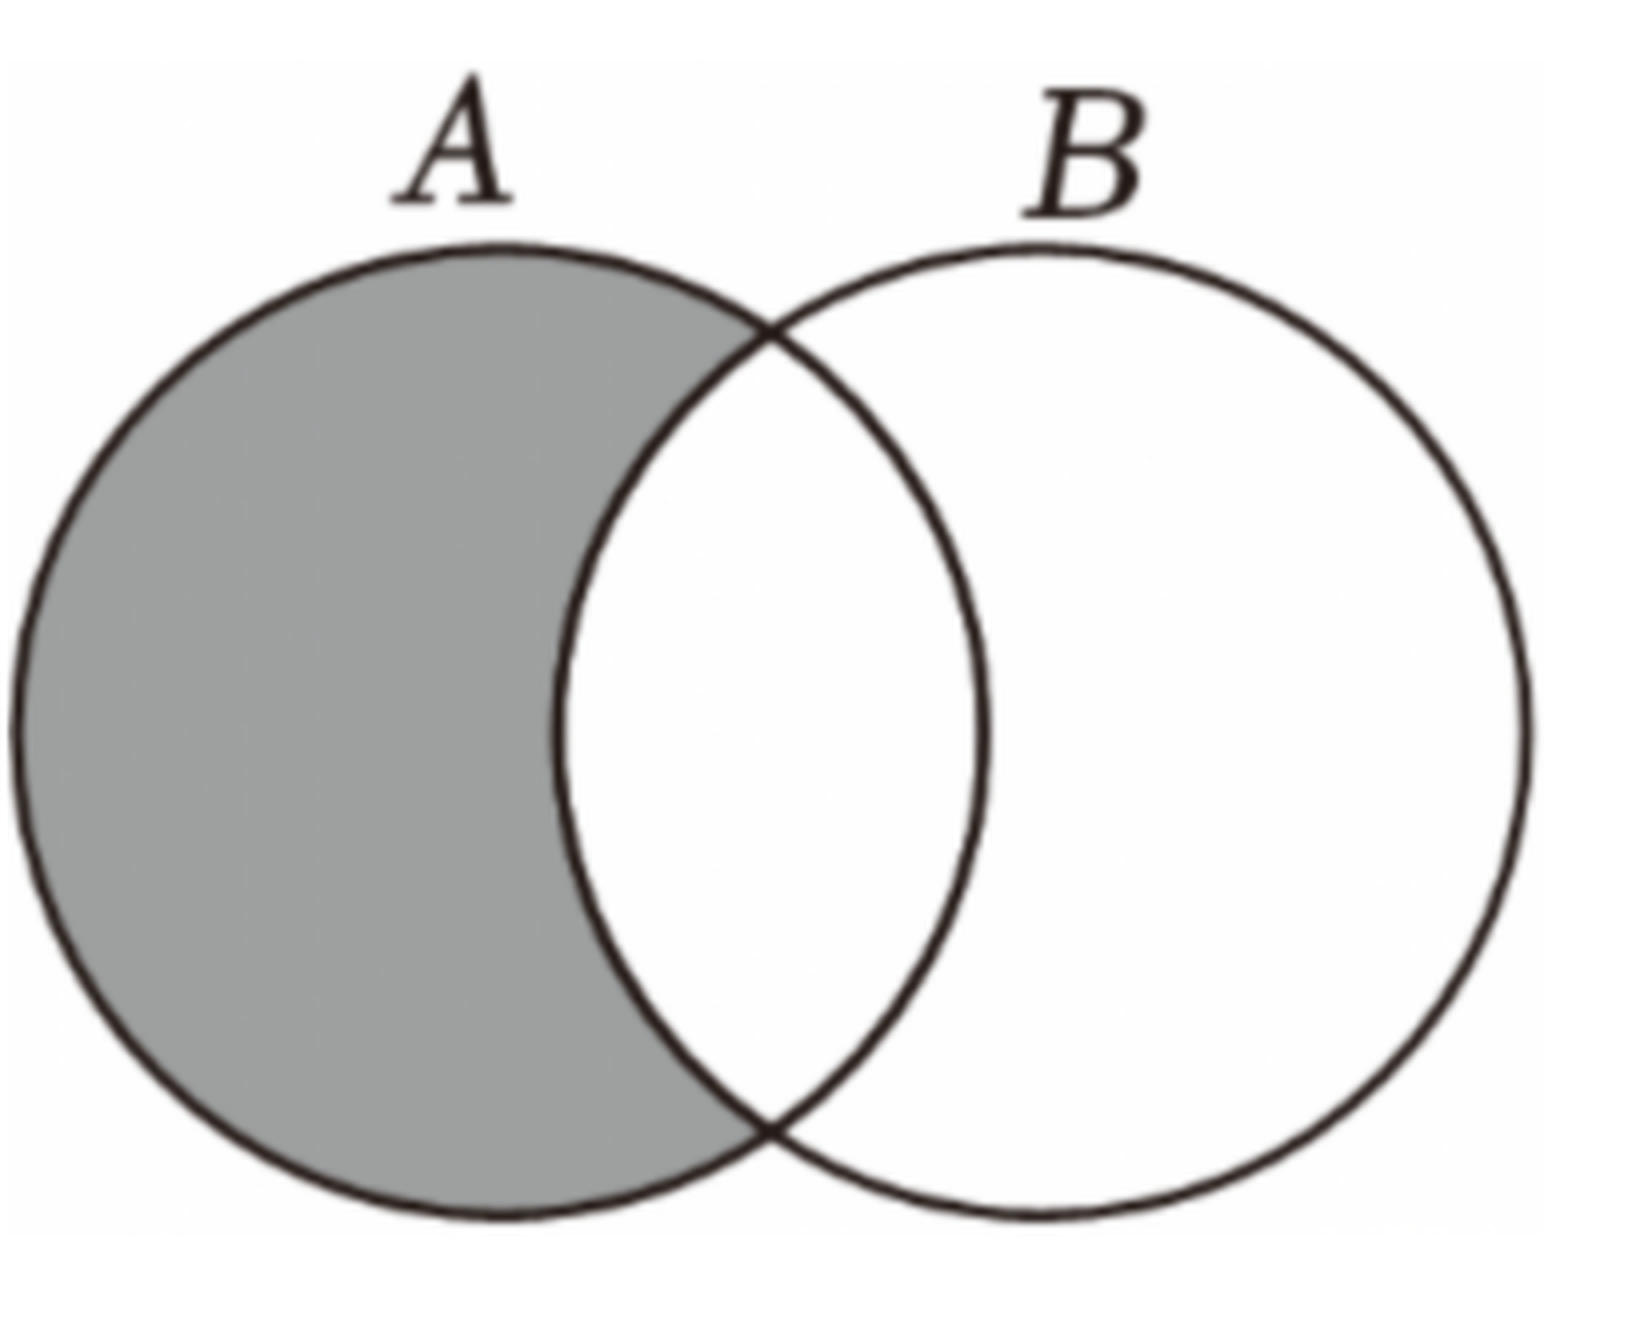
\includegraphics[width=0.30\textwidth]{figures/venn_A_minus_B_h38.png}
\end{center}

\ans{$\{1\}$}

\item 集合 $\{2,3,4,\cdots,2024,2025\}$ 的真子集的个数为 \blankline[4.4em].

\ans{$2^{2024}-1$}

\ifanswer
\solbegin
\step{集合 $\{2,3,4,\cdots,2024,2025\}$ 的真子集的个数为 $2^{2024}-1$.}
\solend

\fi

\item 已知集合 $A$ 中的元素都是正整数，其中最小的是 $1$，最大值是 $100$，除 $1$ 以外，每一个元
素都等于 $A$ 中的两个数（可以相同）的和，则集合 $A$ 中至少含有 \blankline[4.4em] 个元素.

\ans{$9$}

\ifanswer
\solbegin
\step{设 $A$ 中的数从小到大排列为 $1,a_1,a_2,\cdots,a_k,100$，}
\step{则 $a_1=1+1=2$；$3\leqslant a_2\leqslant 4$；$4\leqslant a_3\leqslant 8$；$5\leqslant a_4\leqslant 16$；$6\leqslant a_5\leqslant 32$；$7\leqslant a_6\leqslant 64$；}
\step{于是 $A$ 至少有八个数；}
\step{假设 $A$ 恰好有八个元素，由于 $a_5+a_6\leqslant 96<100$；}
\step{故必须有 $100=a_6+a_6$，$a_6=50$，}
\step{又 $a_4+a_5\leqslant 48$，同理 $a_5=25$，}
\step{但此时 $a_3+a_4\leqslant 24$，$a_5=2a_4$，$a_4=12.5$ 矛盾，}
\step{故 $A$ 不可能恰好有八个元素，因此 $A$ 至少有九个元素.}
\step{其九个数可以为 $1$，$2$，$3$，$6$，$12$，$13$，$25$，$50$，$100$.}
\solend

\fi

\item 已知集合 $\{x_1,x_2,x_3,x_4,x_5,x_6\}=\{1,2,3,4,5,6\}$，将 $x_i$ 与 $x_j$（其中 $i\in\{1,2,3\}$，
$j\in\{4,5,6\}$）的乘积 $x_ix_j$ 放入如图的 $3\times3$ 方格中，则方格中全部数之和的最大值为 \blankline[4.4em].

% 原卷的 $3\times3$ 方格是表格式内容（三行三列的公式），本稿按 高一03 的成例用 tabular 排出。
\begin{center}
\begin{tabular}{|c|c|c|}
\hline
$x_1x_4$ & $x_1x_5$ & $x_1x_6$ \\
\hline
$x_2x_4$ & $x_2x_5$ & $x_2x_6$ \\
\hline
$x_3x_4$ & $x_3x_5$ & $x_3x_6$ \\
\hline
\end{tabular}
\end{center}

\ans{$110$}

\ifanswer
\solbegin
\step{由表格数据得所有数之和为}
\step{$S=x_1x_4+x_1x_5+x_1x_6+x_2x_4+x_2x_5+x_2x_6+x_3x_4+x_3x_5+x_3x_6$，}
\step{所以 $S=(x_1+x_2+x_3)(x_4+x_5+x_6)$，}
\step{因为集合 $\{x_1,x_2,x_3,x_4,x_5,x_6\}=\{1,2,3,4,5,6\}$，}
\step{所以 $x_1+x_2+x_3+x_4+x_5+x_6=1+2+3+4+5+6=21$，}
\step{设 $t=x_1+x_2+x_3$，则 $6\leqslant t\leqslant 15$，$t\in\N^*$，}
\step{$S=t(21-t)=-\left(t-\dfrac{21}{2}\right)^2+\dfrac{441}{4}$，}
\step{当 $t=10$ 或 $t=11$ 时，$S=t(21-t)$ 取最大值，最大值为 $110$，}
\step{此时 $\{x_1,x_2,x_3\}=\{1,4,5\}$，$t=10$，所以可取最大值 $110$.}
\solend

\fi

\item 若 $[x]$ 表示不大于 $x$ 的最大整数，方程 $x^2-8[x]+7=0$ 的解集为 \blankline[4.4em].

\ans{$\{1,\sqrt{33},\sqrt{41},7\}$}

\ifanswer
\solbegin
\step{由题意，$x\geqslant[x]=\dfrac{x^2+7}{8}>0$，得 $x^2-8x+7\leqslant 0$，解得 $1\leqslant x\leqslant 7$，}
\step{$[x]=1$，$x^2=1$，$x=1$；}
\step{$[x]=2$，$x^2=9$，$x=3$ 与 $[x]=2$ 矛盾；}
\step{$[x]=3$，$x^2=17$，$x=\sqrt{17}$，$[x]=4$ 与 $[x]=3$ 矛盾；}
\step{$[x]=4$，$x^2=25$，$x=5$ 与 $[x]=4$ 矛盾；}
\step{$[x]=5$，$x^2=33$，$x=\sqrt{33}$，$[x]=5$；}
\step{$[x]=6$，$x^2=41$，$x=\sqrt{41}$，$[x]=6$；}
\step{$[x]=7$，$x^2=49$，$x=7$；}
\step{综上，方程 $x^2-8[x]+7=0$ 的解集为 $\{1,\sqrt{33},\sqrt{41},7\}$.}
\solend

\fi

\end{enumerate}

\bigsec{二、选择题}

\begin{enumerate}
\setcounter{enumi}{10}

\item 已知集合 $A=\{a,a^2\}$，$B=\{1,3\}$，若 $1\in A$，则 $A\cup B$ 中所有元素之和为\mbox{（\quad）}

\keepwithprev
A. $2$\qquad B. $3$\qquad C. $4$\qquad D. $5$

\ans{$B$}

\ifanswer
\solbegin
\step{因为 $1\in A$，集合 $A=\{a,a^2\}$，所以 $a=1$ 或 $a^2=1$，}
\step{若 $a=1$，则 $a=a^2$，与元素的互异性矛盾；}
\step{若 $a^2=1$，则 $a=1$（舍）或 $a=-1$，故 $A=\{-1,1\}$，$B=\{1,3\}$，}
\step{故 $A\cup B=\{-1,1,3\}$，所以 $A\cup B$ 中所有元素之和为 $-1+1+3=3$. 故选 $B$.}
\solend

\fi

\item 对于实数 $a$、$b$、$c$，下列命题正确的是\mbox{（\quad）}

\keepwithprev
A. 若 $a>b$，则 $ac^2>bc^2$\qquad B. 若 $a>b$，则 $a^2>b^2$

C. 若 $a>b$，则 $a|a|>b|b|$\qquad D. 若 $a>b>c>0$，则 $\dfrac{b}{a-b}<\dfrac{c}{a-c}$

\ans{$C$}

\ifanswer
\solbegin
\step{对于 $A$，若 $a>b$，$c=0$，则 $ac^2=bc^2$，故 $A$ 错误；}
\step{对于 $B$，若 $a>b$，取 $a=-1$，$b=-2$，则 $a^2<b^2$，故 $B$ 错误；}
\step{对于 $C$，若 $a>b>0$ 时，$a|a|-b|b|=a^2-b^2>0$，}
\step{当 $a>0>b$ 时，$a|a|-b|b|=a^2+b^2>0$，}
\step{当 $0>a>b$ 时，$a|a|-b|b|=b^2-a^2=(b-a)(b+a)>0$，}
\step{综上，若 $a>b$，则 $a|a|>b|b|$，故 $C$ 正确；}
\step{对于 $D$，若 $a>b>c>0$，$\dfrac{b}{a-b}-\dfrac{c}{a-c}=\dfrac{ab-bc-ac+bc}{(a-b)(a-c)}=\dfrac{a(b-c)}{(a-b)(a-c)}>0$，}
\step{故 $D$ 错误.}
\step{故选 $C$.}
\solend

\fi

\item 对于正整数集合 $A=\{a_1,a_2,\cdots,a_n\}(n\in\N^*,\ n\geqslant 3)$，如果去掉其中任意一个元素
$a_i(i=1,2,\cdots,n)$ 之后，剩余的所有元素组成的集合都能分为两个交集为空集的集合，且这
两个集合的所有元素之和相等，就称集合 $A$ 为平衡集. 记 $M=a_1+a_2+\cdots+a_n$. 若集合 $A$
是平衡集，并且存在 $a_i$ 为奇数，则集合 $A$ 中元素个数 $n$ 的奇偶性\mbox{（\quad）}

\keepwithprev
A. 与 $M$ 相关，既可以是奇数，又可以是偶数

B. 与 $M$ 无关，既可以是奇数，又可以是偶数

C. 与 $M$ 无关，必为偶数

D. 与 $M$ 无关，必为奇数

\ans{$D$}

\ifanswer
\solbegin
\step{正整数集合 $A=\{a_1,a_2,\cdots,a_n\}(n\in\N^*,\ n\geqslant 3)$，}
\step{因为集合 $A$ 是平衡集，设去掉元素 $a_i(i=1,2,\cdots,n)$，}
\step{由题意得 $A=A_1\cup A_2\cup\{a_i\}$，其中 $A_1\cap A_2=\varnothing$，}
\step{设集合 $A_1$ 和 $A_2$ 中的元素之和均为 $m$，所以 $M=2m+a_i$，其中 $i=1,2,\cdots,n$，}
\step{所以 $M-a_i=2m$，所以 $M-a_i$ 为偶数，其中 $i=1,2,\cdots,n$，}
\step{所以 $a_i(i=1,2,\cdots,n)$ 的奇偶性相同；}
\step{因为存在 $a_i$ 为奇数，所以 $a_i(i=1,2,\cdots,n)$ 均为奇数，}
\step{由 $M-a_i=2m$ 得 $M$ 也为奇数，且 $M=a_1+a_2+\cdots+a_n$，}
\step{所以 $n$ 也为奇数，所以 $n$ 必为奇数. 故选 $D$.}
\solend

\fi

\item 对于集合 $M=\{a\mid a=x^2-y^2,\ x\in\Z,\ y\in\Z\}$，给出如下三个结论：其中正确结论的个数
是\mbox{（\quad）}

\keepwithprev
①如果 $P=\{b\mid b=2n+1,\ n\in\Z\}$，那么 $P\sub M$；

②如果 $c=4n+2$，$n\in\Z$，那么 $c\notin M$；

③如果 $a_1\in M$，$a_2\in M$，那么 $a_1a_2\in M$.

\keepwithprev
A. $1$\qquad B. $2$\qquad C. $3$\qquad D. $0$

\ans{$C$}

\ifanswer
\solbegin
\step{对于①，$b=2n+1$，$n\in\Z$，则恒有 $2n+1=(n+1)^2-n^2$，}
\step{所以 $2n+1\in M$，即 $P=\{b\mid b=2n+1,n\in\Z\}$，则 $P\sub M$，①正确；}
\step{对于②，$c=4n+2$，$n\in\Z$，}
\step{若 $4n+2\in M$，则存在 $x$、$y\in\Z$ 使得 $x^2-y^2=4n+2$，}
\step{所以 $4n+2=(x+y)(x-y)$，又 $x+y$ 和 $x-y$ 同奇或同偶，}
\step{若 $x+y$ 和 $x-y$ 都是奇数，则 $(x+y)(x-y)$ 为奇数，而 $4n+2$ 是偶数；}
\step{若 $x+y$ 和 $x-y$ 都是偶数，则 $(x+y)(x-y)$ 能被 $4$ 整除，而 $4n+2$ 不能被 $4$ 整除，}
\step{所以 $4n+2\notin M$，即 $c\notin M$，②正确；}
\step{对于③，$a_1\in M$，$a_2\in M$，可设 $a_1=x_1^2-y_1^2$，$a_2=x_2^2-y_2^2$，$x_i$、$y_i\in\Z$；}
\step{则 $a_1a_2=(x_1^2-y_1^2)(x_2^2-y_2^2)=(x_1x_2)^2+(y_1y_2)^2-(x_1y_2)^2-(x_2y_1)^2$}
\step{$=(x_1x_2+y_1y_2)^2-(x_1y_2+x_2y_1)^2\in M$，那么 $a_1a_2\in M$，③正确.}
\step{综上，正确的命题是①②③. 故选 $C$.}
\solend

\fi

\end{enumerate}

\bigsec{三、解答题}

\begin{enumerate}
\setcounter{enumi}{14}

\item 已知 $A=\{x\mid a\leqslant x\leqslant -a+3\}$，$B=\{x\mid x<-1\text{ 或 }x>5\}$.

\begin{enumerate}[label=(\arabic*)]

\item 若 $A\cap B=\varnothing$，求 $a$ 的取值范围；

\item 若 $A\cup B=\R$，求 $a$ 的取值范围.

\end{enumerate}

\ans{（1）$[-1,+\infty)$；（2）$(-\infty,-2]$}

\ifanswer
\solbegin
\stepm{(1)}{①当 $A=\varnothing$ 时，$A\cap B=\varnothing$，需满足 $a>-a+3$，解得 $a>\dfrac32$，}
\step{故 $a$ 的取值范围为 $\left(\dfrac32,+\infty\right)$.}
\step{②当 $A\neq\varnothing$ 时，要使 $A\cap B=\varnothing$，需满足
$\begin{cases}a\leqslant\dfrac32\\[4pt] -a+3\leqslant 5\\[4pt] a\geqslant -1\end{cases}$，解得 $-1\leqslant a\leqslant\dfrac32$.}
\step{综上所述，$a$ 的取值范围是 $[-1,+\infty)$.}
\stepm{(2)}{因为 $A\cup B=\R$，$A=\{x\mid a\leqslant x\leqslant -a+3\}$，$B=\{x\mid x<-1\text{ 或 }x>5\}$，}
\step{所以 $\begin{cases}-a+3\geqslant 5\\[4pt] a\leqslant -1\end{cases}$，解得 $a\leqslant -2$，故所求 $a$ 的取值范围为 $(-\infty,-2]$.}
\solend

\fi

\ansspace[6]

\item 已知集合 $A=\{x\mid mx^2+x-2=0\}$，$B=\{x\mid 2x^2-5x-12=0\}$.

\begin{enumerate}[label=(\arabic*)]

\item 若 $A$ 中有且仅有 $1$ 个元素，求实数 $m$ 的值；

\item 已知集合 $C=A\cup B$，若 $C$ 的真子集有且仅有 $3$ 个，求实数 $m$ 的取值范围.

\end{enumerate}

\ans{（1）$m=0$ 或 $m=-\dfrac18$；（2）$\left\{m\mid m\leqslant -\dfrac18\right\}$}

\ifanswer
\solbegin
\stepm{(1)}{若 $m=0$，方程化为 $x-2=0$，此时方程有且仅有一个根 $x=2$；}
\step{若 $m\neq 0$，则 $\Delta=1^2-4\times m\times(-2)=0$，即 $m=-\dfrac18$ 时，}
\step{方程有两个相等的实根，此时集合 $A$ 中有且仅有一个元素，}
\step{所以实数 $m$ 的值为 $m=0$ 或 $m=-\dfrac18$；}
\stepm{(2)}{$B=\{x\mid 2x^2-5x-12=0\}=\left\{-\dfrac32,4\right\}$，}
\step{因为 $C=A\cup B$，若 $C$ 的真子集有且仅有 $3$ 个，则 $C$ 中有两个元素，}
\step{所以 $A\sub B$，由（1）得 $m=0$ 时，$A=\{2\}$，不符合 $A\sub B$，}
\step{当 $m\neq 0$ 时，若 $\Delta=1^2-4\times m\times(-2)<0$，解得 $m<-\dfrac18$，}
\step{此时 $A=\varnothing$，符合 $A\sub B$，}
\step{若 $\Delta=1^2-4\times m\times(-2)=0$，解得 $m=-\dfrac18$，}
\step{此时方程 $mx^2+x-2=0$ 的根为 $x=4$，集合 $A=\{4\}$，符合 $A\sub B$，}
\step{若 $\Delta=1^2-4\times m\times(-2)>0$，由 $A\sub B$，得 $A=\left\{-\dfrac32,4\right\}$，}
\step{此时有 $-\dfrac32+4=-\dfrac1m$ 且 $-\dfrac32\times 4=-\dfrac2m$，无解，}
\step{综上所述，实数 $m$ 的取值范围为 $\left\{m\mid m\leqslant -\dfrac18\right\}$.}
\solend

\fi

\ansspace[6]

\item 设 $A$ 是非空实数集，且 $0\notin A$. 若对于任意的 $x$、$y\in A$，都有 $xy\in A$，则称集合 $A$ 具
有性质 $P_1$；若对于任意的 $x$、$y\in A$，都有 $\dfrac xy\in A$，则称集合 $A$ 具有性质 $P_2$.

\begin{enumerate}[label=(\arabic*)]

\item 写出一个恰含有两个元素且具有性质 $P_1$ 的集合 $A$，并说明理由；

\item 证明：“非空实数集 $A$ 具有性质 $P_1$”是“非空实数集 $A$ 具有性质 $P_2$”的必要非充分条
件.

\end{enumerate}

\ans{（1）$A=\{-1,1\}$，理由见解析；（2）见解析}

\ifanswer
\solbegin
% 注：原卷本题 (1) 的解析里“证明”一词重复出现两次（一次接在分号后、一次另起一行），
%     本稿照原卷重复录入，未去重。
\stepm{(1)}{$A=\{-1,1\}$，证明：恰含有两个元素且具有性质 $P_1$ 的集合 $A=\{-1,1\}$；}
\step{证明：$1\times 1=1\in A$，$1\times(-1)=-1\in A$，$-1\times 1=-1\in A$，$-1\times(-1)=1\in A$；}
\stepm{(2)}{若集合 $A$ 具有性质 $P_2$，不妨设 $a\in A$，}
\step{由非空数集 $A$ 具有性质 $P_2$，有 $\dfrac aa=1\in A$.}
\step{①$A=\{1\}$，易得此时集合 $A$ 具有性质 $P_1$.}
\step{②数集 $A$ 只含有两个元素，不妨设 $A=\{1,a_1\}$，}
\step{由 $\dfrac{1}{a_1}=a_1$，且 $a_1\neq 1$，解得 $a_1=-1$，此时集合 $A$ 具有性质 $P_1$.}
\step{③实数集 $A$ 含有两个以上的元素，不妨设不为 $1$ 的元素 $a_1$、$a_2\in A$，}
\step{则有 $\dfrac{1}{a_1}\in A$，由于集合 $A$ 具有性质 $P_2$，}
\step{所以有 $a_2\div\dfrac{1}{a_1}=a_1a_2\in A$，这说明集合 $A$ 具有性质 $P_1$.}
\step{综上，若非空实数集 $A$ 具有性质 $P_2$，则集合 $A$ 具有性质 $P_1$，}
\step{所以“非空实数集 $A$ 具有性质 $P_1$”是“非空实数集 $A$ 具有性质 $P_2$”的}
\step{必要条件.}
\step{取正偶数集 $A=\{x\mid x=2n,\ n\in\N^*\}$，}
\step{对任意的 $2m$、$2n\in A$，$m$、$n\in\N^*$，}
\step{有 $2m\times 2n=4mn\in A$，故 $A$ 具有性质 $P_1$，}
\step{取 $x=2$，$y=4$，则 $\dfrac xy=\dfrac12\notin A$，故 $A$ 不具有性质 $P_2$，}
\step{所以“非空实数集 $A$ 具有性质 $P_1$”不是“非空实数集 $A$ 具有性质 $P_2$”的}
\step{充分条件.}
\step{综上，“非空实数集 $A$ 具有性质 $P_1$”是“非空实数集 $A$ 具有性质 $P_2$”的}
\step{必要非充分条件.}
\solend

\fi

\ansspace[8]

\item 已知命题 $p$：关于 $x$ 的方程 $x^2+mx+1=0$ 有两个不同的正根；命题 $q$：关于 $x$ 的方程
$4x^2+4(m-2)x=-1$ 有实根.

\begin{enumerate}[label=(\arabic*)]

\item 若命题 $q$ 为假命题，求整数 $m$ 的解集；

\item 若命题 $p$ 为真命题，且关于 $x$ 的方程 $x^2+mx+1=0$ 的两个实数根 $x_1$、$x_2$ 满足
$3x_1+2x_2=5$，求实数 $m$ 的取值集合；

\item 若命题 $p$ 和命题 $q$ 有且仅有一个成立，求实数 $m$ 的取值范围.

\end{enumerate}

\ans{（1）$\{2\}$；（2）$\left\{-\dfrac{13}{6}\right\}$；（3）$[-2,1]\cup[3,+\infty)$}

\ifanswer
\solbegin
\stepm{(1)}{命题 $q$：关于 $x$ 的方程 $4x^2+4(m-2)x=-1$ 有实根为假命题，}
\step{即 $4x^2+4(m-2)x+1=0$ 无实根，}
\step{则 $\Delta=16(m-2)^2-16<0$，则 $1<m<3$，则整数 $m$ 的解集为 $\{2\}$；}
\stepm{(2)}{若命题 $p$ 为真命题，且关于 $x$ 的方程 $x^2+mx+1=0$ 的两个实数根 $x_1$、$x_2$，}
\step{满足 $3x_1+2x_2=5$，则方程 $x^2+mx+1=0$ 有两个不同的正根，}
\step{则 $\begin{cases}\Delta=m^2-4>0\\[4pt] x_1+x_2=-m>0\end{cases}$，则 $m<-2$，}
\step{又 $\begin{cases}x_1+x_2=-m\\[4pt] x_1x_2=1\\[4pt] 3x_1+2x_2=5\end{cases}$，
则 $\begin{cases}x_1=5+2m\\[4pt] x_2=-3m-5\end{cases}$，则 $(5+2m)(-3m-5)=1$，}
\step{得 $m=-2$ 或 $m=-\dfrac{13}{6}$，又因为 $m<-2$，所以 $m=-\dfrac{13}{6}$，}
\step{所以实数 $m$ 的取值集合为 $\left\{-\dfrac{13}{6}\right\}$；}
\stepm{(3)}{由（2）得当 $p$ 为真时，则有 $m<-2$，}
\step{当 $q$ 为真时，$\Delta=16(m-2)^2-16\geqslant 0$，解得 $m\leqslant 1$ 或 $m\geqslant 3$，}
\step{又因为命题 $p$ 和命题 $q$ 只有一个为真，所以
$\begin{cases}m<-2\\[4pt] 1<m<3\end{cases}$ 或 $\begin{cases}m\geqslant -2\\[4pt] m\leqslant 1\text{ 或 }m\geqslant 3\end{cases}$，}
\step{解得 $-2\leqslant m\leqslant 1$ 或 $m\geqslant 3$，所以实数 $m$ 的取值范围为 $[-2,1]\cup[3,+\infty)$.}
\solend

\fi

\ansspace[8]

% 注：原卷此处作“设 $n\in\N^*$，集合含有 $3n$ 个元素”，**漏了符号 $U$**（应作“集合 $U$
%     含有 $3n$ 个元素”）——$U$ 直到本句末尾“则称 $U$ 为三分集合”才出现、此前无定义。
%     本稿照录未补，见文件头“原卷笔误/存疑”⑦。
\item 设 $n\in\N^*$，集合含有 $3n$ 个元素，若存在三个 $n$ 元集合 $A$、$B$、$C$ 满足如下两个条件，
则称 $U$ 为三分集合.

①$U=A\cup B\cup C$；

②$A$、$B$、$C$ 元素可分别排列为有序数组 $(a_1,a_2,\cdots,a_n)$，$(b_1,b_2,\cdots,b_n)$ 及
$(c_1,c_2,\cdots,c_n)$，使得对 $\forall i=1,2,\cdots,n$，均有 $a_i+b_i=c_i$.

特别地，当 $U=\{1,2,3,4,\cdots,3n-2,3n-1,3n\}$ 为三分集合时，称 $n$ 为完美三分数.

如：因为 $U=\{1,2,3\}$ 为三分集合，所以 $n=1$ 为最小完美三分数.

\begin{enumerate}[label=(\arabic*)]

\item 请判断下列两个集合是否为三分集合（直接写出结论）：

$U_1=\{1,2,3,4,5,6\}$，$U_2=\{1,3,5,7,8,9,10,11,12\}$；

\item 求出大于 $1$ 的最小完美三分数；

\item 请判断是否存在无穷多个完美三分数？若存在，请说明理由；若不存在，则求出最大的
完美三分数.

\end{enumerate}

\ans{（1）$U_1$ 不是三分集合，$U_2$ 是三分集合；（2）$4$；（3）存在，理由见解析}

\ifanswer
\solbegin
\stepm{(1)}{(i)$U_1=\{1,2,3,4,5,6\}$ 不是三分集合，下面用反证法证明：}
\step{证明：假设 $U=\{1,2,3,4,5,6\}$ 是三分集合，}
\step{设 $A=\{a_1,a_2\}$，$B=\{b_1,b_2\}$，$C=\{c_1,c_2\}$，不妨设 $c_1<c_2$，}
\step{因为 $a_1+b_1=c_1$，$a_2+b_2=c_2$，}
\step{所以 $a_1+b_1+a_2+b_2+c_1+c_2=2(c_1+c_2)=1+2+3+4+5+6=21$，}
% 注：原卷此步印“所以 $c_1+c_2=2$”，与上一行的 $2(c_1+c_2)=21$ **不自洽**
%     （应作 $\dfrac{21}2$）；同题 $n=3$ 处的同型推理原卷写的是 $\dfrac{45}2$，故此处是原卷笔误。
%     本稿照录未改，见文件头“原卷笔误/存疑”⑧。
\step{所以 $c_1+c_2=2$，这与 $c_1,c_2\in\N^*$ 矛盾，故假设错误，}
\step{故 $U_1=\{1,2,3,4,5,6\}$ 不是三分集合；}
\step{(ii)$U_2=\{1,3,5,7,8,9,10,11,12\}$ 是三分集合，理由如下：}
\step{令 $A=\{1,3,5\}$，$B=\{9,8,7\}$，$C=\{10,11,12\}$，}
\step{则 $A\cup B\cup C=U=\{1,3,5,7,8,9,10,11,12\}$，满足条件①；}
\step{又 $1+9=10$；$3+8=11$；$5+7=12$，所以满足条件②，}
\step{所以 $U_2=\{1,3,5,7,8,9,10,11,12\}$ 是三分集合；}
\stepm{(2)}{由（1）得，当 $n=2$ 时，$U=\{1,2,3,4,5,6\}$ 不是三分集合；}
\step{当 $n=3$ 时，$U=\{1,2,3,4,5,6,7,8,9\}$，}
\step{假设 $U=\{1,2,3,4,5,6,7,8,9\}$ 是三分集合，}
\step{同理由 $a_1+b_1+a_2+b_2+a_3+b_3+c_1+c_2+c_3$}
\step{$=2(c_1+c_2+c_3)=1+2+\cdots+9=45$，$c_1+c_2+c_3=\dfrac{45}{2}$，}
\step{可推出与 $c_1$、$c_2$、$c_3\in\N^*$ 矛盾，故假设也错误，}
\step{所以 $U=\{1,2,3,4,5,6,7,8,9\}$ 不是三分集合；}
\step{当 $n=4$ 时，$U=\{1,2,3,\cdots,12\}$，}
\step{存在三个 $4$ 元集合 $A=\{1,2,4,3\}$，$B=\{5,8,7,9\}$，$C=\{6,10,11,12\}$，}
\step{满足 $U=\{1,2,3,\cdots,12\}$ 为三分集合的两个条件，}
\step{故大于 $1$ 的最小完美三分数为 $4$；}
\stepm{(3)}{存在无穷多个完美三分数，理由如下：}
\step{由题意得，$n=1$ 为最小完美三分数，}
\step{当 $n=5$ 时，$U=\{1,2,3,\cdots,15\}$，}
\step{存在三个 $5$ 元集合 $A=\{1,3,5,7,2\}$，$B=\{11,10,9,8,4\}$，$C=\{12,13,14,15,6\}$，}
\step{满足三分集合的条件，故 $5$ 为完美三分数；}
\step{当 $n=21$ 时，$U=\{1,2,3,\cdots,63\}$，}
\step{存在如下三个 $21$ 元的集合满足三分集合的条件：}
\step{$A=\{1,3,5,7,\cdots,29,31,2,6,10,14,4\}$，}
\step{$B=\{47,46,45,44,\cdots,33,32,22,20,18,16,8\}$，}
\step{$C=\{48,49,50,51,\cdots,62,63,24,26,28,30,12\}$，}
\step{故 $21$ 为完美三分数.}
\step{首先证明：若 $n=k$，$k\in\N^*$ 为三分完美数，}
\step{则 $n=4k+1$，$k\in\N^*$ 也为三分完美数，}
% 注：下一行原卷印作“$U_{k+1}=U_{k+1}=\{2,3,\cdots,12k+3\}$”——等号两边记号相同，
%     依上下文疑当作 $U'_{k+1}=U_{4k+1}$，且此处集合自 2 起（前文 $U_{4k+1}$ 自 1 起）；
%     本稿照录原卷，未代为改写。
\step{证明：记 $U_k=\{1,2,3,\cdots,3k\}$，$U_{4k+1}=\{1,2,3,\cdots,12k+3\}$，}
\step{若 $n=k$，$k\in\N^*$ 为三分完美数，则 $U_k$ 为三分集合，}
\step{即存在三个 $k$ 元集合 $A$、$B$、$C$ 满足如下两个条件，}
\step{①$U_k=A\cup B\cup C$；}
\step{②$A$、$B$、$C$ 元素可分别排列为有序数组 $(a_1,a_2,\cdots,a_k)$，}
\step{$(b_1,b_2,\cdots,b_k)$ 及 $(c_1,c_2,\cdots,c_k)$，}
\step{使得对 $\forall i=1,2,3,\cdots,k$，均有 $a_i+b_i=c_i$，}
\step{则可得到对 $\forall i=1,2,3,\cdots,k$，$2a_i+2b_i=2c_i$，}
\step{故集合 $\{2,4,6,\cdots,6k\}$ 也满足三分集合的两个条件，其也为三分集合，}
\step{下面记集合 $\{2,4,6,\cdots,6k\}=2U_k$，}
\step{对 $n=4k+1$，集合 $U_{k+1}=U_{k+1}=\{2,3,\cdots,12k+3\}=(2U_k)\cup\complement_{U_{4k+1}}(2U_k)$，}
\step{构造集合 $A'=\{1,3,5,7,\cdots,6k+1\}$，共有 $3k+1$ 个奇数；}
% 注：下一行原卷印作“$B'=\{6k+3k+2,6k+3k+1,6k+3k,6k+3k-1,\cdots,6k+2\}$”，
%     按与后文 $C'$ 相接，前四项当写作 $9k+2$、$9k+1$、$9k$、$9k-1$；本稿照录原卷。
\step{集合 $B'=\{6k+3k+2,6k+3k+1,6k+3k,6k+3k-1,\cdots,6k+2\}$，}
\step{共有 $3k+1$ 个逐个减小的连续正整数；}
\step{集合 $C'=\{9k+3,9k+4,9k+5,9k+6,\cdots,12k+3\}$，}
\step{共有 $3k+1$ 个逐个增大的连续正整数；}
\step{得这三个 $3k+1$ 元集合 $A'$、$B'$、$C'$ 满足如下两个条件，}
\step{①集合 $A'\cup B'\cup C'=\complement_{U_{4k+1}}(2U_k)$；}
\step{②$A'$、$B'$、$C'$ 元素可分别排列为有序数组 $(a_1,a_2,\cdots,a_{3k+1})$，}
\step{$(b_1,b_2,\cdots,b_{3k+1})$ 及 $(c_1,c_2,\cdots,c_{3k+1})$，}
\step{使得对 $\forall i=1,2,3,\cdots,3k+1$，均有 $a_i+b_i=c_i$；}
\step{故 $\complement_{U_{4k+1}}(2U_k)$ 为三分集合，而已知 $U_k$ 为三分集合，}
\step{将其对应与 $A'$、$B'$、$C'$ 合并，}
% 注：原卷此处印“令 $A''=A\cup A'$”（$B''$、$C''$ 同）。按同段上文“记集合
%     $\{2,4,6,\cdots,6k\}=2U_k$”，此处疑当作 $A''=2A\cup A'$——否则
%     $A''\cup B''\cup C''=U_k\cup\complement_{U_{4k+1}}(2U_k)\neq U_{4k+1}$，与本段结论冲突。
%     本稿照录未改，见文件头“原卷笔误/存疑”⑨。
\step{令 $A''=A\cup A'$，$B''=B\cup B'$，$C''=C\cup C'$，}
\step{则这三个 $4k+1$ 元集合 $A''$、$B''$、$C''$，}
\step{满足 $A''\cup B''\cup C''=U_{4k+1}$，且满足条件②，}
\step{故 $U_{4k+1}=\{1,2,3,\cdots,12k+3\}$ 为三分集合，}
\step{因此可得，若 $n=k$ 为三分完美数，则 $n=4k+1$ 也为三分完美数，}
\step{由 $1$，$5$，$21$ 为完美三分数，结合所证结论得，存在无穷多个完美三分数.}
\solend

\fi

\ansspace*[12]

\end{enumerate}

\end{document}
"
% 紧凑版：xelatex "\def\iscompact{1}% 高一38_大同中学_周末作业3.tex
%   —— 高一上数学“2026-2027 年大同中学高一上周末作业 3”（试卷版/答案版）
% 试卷版：xelatex 高一38_大同中学_周末作业3.tex
% 答案版：xelatex "\def\isanswer{1}% 高一38_大同中学_周末作业3.tex
%   —— 高一上数学“2026-2027 年大同中学高一上周末作业 3”（试卷版/答案版）
% 试卷版：xelatex 高一38_大同中学_周末作业3.tex
% 答案版：xelatex "\def\isanswer{1}% 高一38_大同中学_周末作业3.tex
%   —— 高一上数学“2026-2027 年大同中学高一上周末作业 3”（试卷版/答案版）
% 试卷版：xelatex 高一38_大同中学_周末作业3.tex
% 答案版：xelatex "\def\isanswer{1}\input{高一38_大同中学_周末作业3.tex}"
% 紧凑版：xelatex "\def\iscompact{1}\input{高一38_大同中学_周末作业3.tex}"
%
% 原始材料是微信公众号图文（公众号“魔都数学加油站”连载“27学年高一 38”，署名“破晓”，
% 2026-09-26 21:29 发布，原文标题“27学年高一38——2026-2027年上海市大同中学高一上周末作业3”，
% 原文链接 https://mp.weixin.qq.com/s/O_O60vCIiGi2xponAo4irw ），正文为 12 张 PNG 页。
% **同一篇里各页分辨率不一致**（2560×3620 与 4762×6735 两档混排：第 1、10、11、12 页为
% 2560×3620，第 2—9 页为 4762×6735）。原文本身就是一份**讲评版**——有的题下方只印
% 【答案】行，有的只印【解析】。试题文字、答案与解析均照原卷录入，未改内容。卷面的粉色
% 斜水印“魔都数学加油站”属水印，未录入。
%
% 本卷共 **17 题**：填空题 8 题（第 3—10 题）、选择题 4 题（第 11—14 题）、解答题 5 题
% （第 15—19 题）；插图 1 张（第 6 题 Venn 图）。三版页数：试卷版 4 页 / 答案版 11 页 /
% 紧凑版 3 页，`Overfull`／`Underfull`／`Missing character` 告警均为 0。
%
% 卷首标题：原卷印作“2026-2027 年大同中学高一上周末作业 3”（公众号原文标题里的“上海市”
% 三字卷面标题行没有，本稿照卷面），年份区间按全稿惯例排 en dash，前缀照原卷保留“年”。
%
% 与原卷的排版差异（均已在 README“说明”中交代）：
%   ① 原文自**第 3 题**起（第 1、2 题未在该文中发布），故本稿题号亦自 3 起，填空题以
%      \setcounter{enumi}{2} 起编；选择、解答两节各按上一节末号另设 \setcounter
%      （选择题 \setcounter{enumi}{10}、解答题 \setcounter{enumi}{14}）；
%   ② 原卷本就印有“一、填空题”“二、选择题”“三、解答题”三节标题，本稿照原卷分节，
%      只把标题改排成全稿统一的“大节标题”样式；
%   ③ 原卷是“讲评版”：第 3、6 题只印【答案】行，第 4、5、7、8、9、10 题与第 11—19 题印
%      【解析】；本稿统一改为试卷版隐去、答案版以 \ans{}／\ifanswer 块给出，两版彻底分离。
%      其中第 4、5、7、8、9、10 题与第 11—14 题的答案，原卷写在【解析】末句，本稿另提为
%      \ans{}；第 15—19 题原卷只有【解析】、无独立答案行，本稿亦补了摘要式 \ans{}。
%      **故本卷 17 题每题都有 \ans**——比“只印【解析】的填空、解答题不另提 \ans”的
%      高一31／高一34 更彻底，与 高一21 第 11 题（填空，答案在【解析】末句，本稿另提）同类；
%      （本仓对“另提 \ans{}”的做法各卷不一，见 README 对应专记的核对面。）
%   ④ 数集记号原卷两套并用：第 3、5 题的实数集作粗体 $\mathbf{R}$，第 8、14、17、18 题等的
%      整数集、自然数集作斜体 $Z$、$N$，本稿按全稿惯例统一写作 $\R$、$\Z$、$\N$；
%   ⑤ 原卷填空的横线宽度不一（约 1.8—3.6 字宽），本稿按全稿惯例统一排 \blankline[4.4em]；
%   ⑥ 中文括注原卷用半角“(  )”，本稿按全稿惯例排全角；选择题的作答括注统一排
%      \mbox{（\quad）}（第 14 题的作答括注原卷印在 ①②③ 三个命题**之前**，本稿照原卷次序）；
%      数学式内部的括注（如第 4 题的 $p\%(0<p<100)$、第 13 题的 $a_i(i=1,2,\cdots,n)$）照原样
%      留在行内公式里，未改全角；
%   ⑦ 原卷并列的字母（“x,y”“a,b,c”）不加标点或作半角逗号，本稿按全稿惯例改排顿号；
%   ⑧ 第 6 题的 Venn 图取原卷截图、4× LANCZOS 放大（figures/venn_A_minus_B_h38.png，
%      见该处 \includegraphics 前的注释）；第 9 题的 $3\times3$ 方格属**表格式**内容，
%      本稿按 高一03 的成例用 tabular 排出，未截图；
%   ⑨ 原卷未印副标题，本稿按**本卷实际内容**补出副标题“集合与常用逻辑用语”（依据见下条）；
%   ⑩ 原卷【解析】**一个印刷行照录为一条 `\step`**（原卷的折行也照录为独立一条，如第 17 题
%      末三处“…的”／“必要条件.”这类跨行句、第 9 题“由表格数据得所有数之和为”／
%      “$S=\cdots$，”），使答案版的排布与原卷讲评版逐行对应；全卷 15 处【解析】合计
%      **191 条 `\step` ＝ 原卷 191 行**（逐处：5、5、1、9、9、9、4、9、9、12、6、14、21、13、65）。
%
% 副标题（\examtitlest 第二个参数）：本卷卷面未印副标题，由本稿补出，取值按 2026-09-26 起的
%   新口径“只用本卷实际内容的模块名”定为“集合与常用逻辑用语”。依据：全卷 17 题
%   （第 3—19 题）中，第 3、5、6、7、8、9、10、11、13、14、15、16、17、18、19 题共 15 题
%   是集合的运算与关系、子集计数、集合新定义（性质 $P_1$／$P_2$、平衡集、三分集合），以及
%   命题与逻辑（第 3 题即用反证法证明“$x+y>2\Rightarrow x>1$ 或 $y>1$”这一命题）；不等式只
%   出现在第 4 题（降价提价的应用比较）、第 12 题（不等式命题真假）与第 10 题解析里解一元
%   二次不等式，合计不足全卷的三分之一，故不并标“不等式”。
%
% 原卷笔误/存疑（均照抄原卷、未改，见源码中该处上方注释）：
%   ① 第 19 题 (3) 的证明里印作“集合 $U_{k+1}=U_{k+1}=\{2,3,\cdots,12k+3\}$”——等号两边
%      记号相同（依上下文疑当作 $U'_{k+1}=U_{4k+1}$），且此处集合自 $2$ 起，而前文
%      $U_{4k+1}=\{1,2,3,\cdots,12k+3\}$ 自 $1$ 起；本稿照录；
%   ② 第 19 题 (3) 的证明里印作
%      “$B'=\{6k+3k+2,6k+3k+1,6k+3k,6k+3k-1,\cdots,6k+2\}$”——按与后文
%      $C'=\{9k+3,9k+4,9k+5,9k+6,\cdots,12k+3\}$ 相接，前四项当写作 $9k+2$、$9k+1$、
%      $9k$、$9k-1$（即 $6k+3k+2$ 等），原卷即作“$6k+3k+\cdots$”形式，本稿照录；
%   ③ 第 19 题的术语前后不一：题干与 (1)(2)(3) 用“完美三分数”，而 (3) 的证明里五次写作
%      “三分完美数”（词序不同）；本稿五处都照录；
%   ④ 第 14 题题干作“给出如下三个结论：其中正确结论的个数是（\quad）”，此处冒号疑当作
%      逗号，本稿照录；
%   ⑤ 第 17 题题干作“非空实数集”，其解析有一处写作“非空数集”；本稿照录；
%   ⑥ 第 17 题 (1) 的【解析】原卷连写“…集合 $A=\{-1,1\}$；证明：…；证明：…”，“证明”
%      一词重复出现两次（第一次在分行处、第二次另起一行），本稿照原卷重复录入，未去重。
%   ⑦ 第 19 题**题干漏字**：原卷作“19.设 $n\in\N^*$，集合含有 $3n$ 个元素…则称 $U$ 为
%      三分集合”——首句漏了符号 $U$（应作“集合 $U$ 含有 $3n$ 个元素”），$U$ 直到结论句
%      才出现、此前无定义；本稿照录未补（见该处上方注释）。
%   ⑧ 第 19(1)(i) 的【解析】**自相矛盾**：上一行印“$a_1+b_1+a_2+b_2+c_1+c_2=2(c_1+c_2)
%      =1+2+3+4+5+6=21$”，下一行却印“所以 $c_1+c_2=2$”（由 $2(c_1+c_2)=21$ 应得
%      $c_1+c_2=\dfrac{21}2$，非整数、才与 $c_1,c_2\in\N^*$ 矛盾）；同题 $n=3$ 处的同型
%      推理原卷就写对了（$\dfrac{45}2$），故此处是原卷笔误；本稿照录未改（见该处上方注释）。
%   ⑨ 第 19(3) 的【解析】印“令 $A''=A\cup A'$，$B''=B\cup B'$，$C''=C\cup C'$”——按同段
%      上文“记集合 $\{2,4,6,\cdots,6k\}=2U_k$”，$A''$ 等疑当作 $2A\cup A'$（$B''$、$C''$ 同），
%      否则 $A''\cup B''\cup C''=U_k\cup\complement_{U_{4k+1}}(2U_k)\neq U_{4k+1}$；本稿照录未改
%      （见该处上方注释）。

\documentclass[a4paper,11pt]{article}
\usepackage{common}

\begin{document}

\examtitlest[3]{2026--2027 年大同中学高一上周末作业 3}{集合与常用逻辑用语}

\bigsec{一、填空题}

\begin{enumerate}
% 原卷填空题自第 3 题起（第 1、2 题未在该文中发布），须与选择、解答两节的 \setcounter 对齐
\setcounter{enumi}{2}

\item 设 $x$、$y\in\R$，若 $x+y>2$，则 $x>1$ 或 $y>1$ 是真命题. 这个命题可以用反证法去证明，
可以假设：\blankline[4.4em].

\ans{$x\leqslant 1$ 且 $y\leqslant 1$}

\item 已知某商品的原价为 $a$ 元，由于市场原因，先降价 $p\%(0<p<100)$ 出售，一段时间后，
再提价 $p\%$ 出售，则该商品提价后的售价 \blankline[4.4em] 该商品的原价（填“高于”“低于”或“等于”）.

\ans{低于}

\ifanswer
\solbegin
\step{由题意得第一次降价后的售价为 $a(1-p\%)$ 元，}
\step{第二次提价后的售价为 $a(1-p\%)(1+p\%)$ 元，}
\step{因为 $0<p<100$，所以 $0<p\%<1$，}
\step{因为 $a(1-p\%)(1+p\%)=a[1-(p\%)^2]<a$，}
\step{即该商品提价后的售价低于该商品的原价.}
\solend

\fi

\item 若集合 $A=\{x\mid ax^2+ax+1=0,\ a\in\R,\ x\in\R\}$ 的子集只有两个，则实数 $a=$ \blankline[4.4em].

\ans{$4$}

\ifanswer
\solbegin
\step{集合 $A=\{x\mid ax^2+ax+1=0\}$ 的子集只有两个，}
\step{所以 $A$ 有且只有一个元素，}
\step{①若 $a=0$，则 $A=\varnothing$ 不成立；}
\step{②若 $a\neq 0$，则 $\Delta=a^2-4a=0$，解得 $a=4$（$0$ 舍）.}
\step{故 $a=4$.}
\solend

\fi

\item 如图，已知集合 $A=\{1,2,3,4,5\}$，集合 $B=\{2,3,4,5,9\}$，则图中阴影部分所表示的
集合为 \blankline[4.4em].

% 图取原卷截图（01.png，2560×3620）右栏，4× LANCZOS 放大；为避免与 高一11 的
% figures/venn_A_minus_B.png 同名，按 高一32 的成例加 _h38 后缀。
\begin{center}
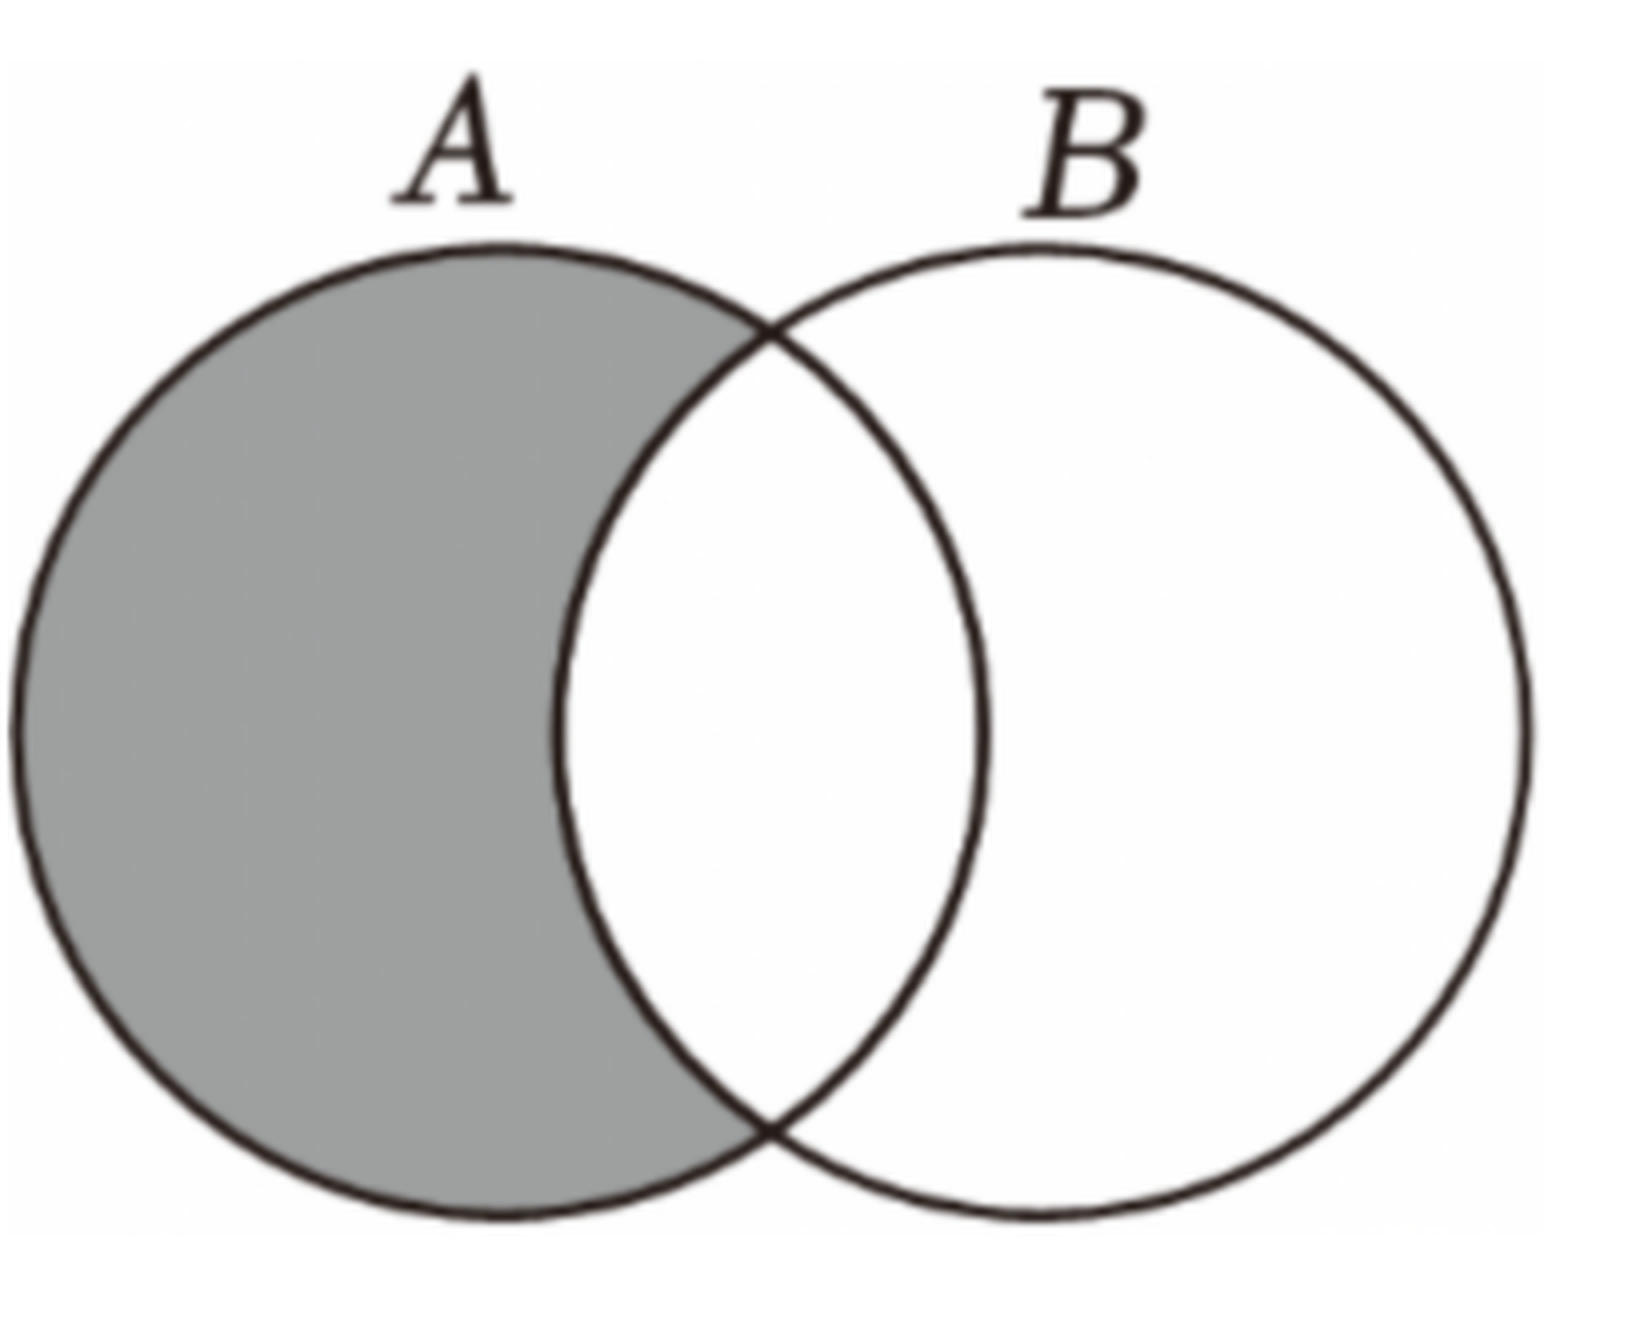
\includegraphics[width=0.30\textwidth]{figures/venn_A_minus_B_h38.png}
\end{center}

\ans{$\{1\}$}

\item 集合 $\{2,3,4,\cdots,2024,2025\}$ 的真子集的个数为 \blankline[4.4em].

\ans{$2^{2024}-1$}

\ifanswer
\solbegin
\step{集合 $\{2,3,4,\cdots,2024,2025\}$ 的真子集的个数为 $2^{2024}-1$.}
\solend

\fi

\item 已知集合 $A$ 中的元素都是正整数，其中最小的是 $1$，最大值是 $100$，除 $1$ 以外，每一个元
素都等于 $A$ 中的两个数（可以相同）的和，则集合 $A$ 中至少含有 \blankline[4.4em] 个元素.

\ans{$9$}

\ifanswer
\solbegin
\step{设 $A$ 中的数从小到大排列为 $1,a_1,a_2,\cdots,a_k,100$，}
\step{则 $a_1=1+1=2$；$3\leqslant a_2\leqslant 4$；$4\leqslant a_3\leqslant 8$；$5\leqslant a_4\leqslant 16$；$6\leqslant a_5\leqslant 32$；$7\leqslant a_6\leqslant 64$；}
\step{于是 $A$ 至少有八个数；}
\step{假设 $A$ 恰好有八个元素，由于 $a_5+a_6\leqslant 96<100$；}
\step{故必须有 $100=a_6+a_6$，$a_6=50$，}
\step{又 $a_4+a_5\leqslant 48$，同理 $a_5=25$，}
\step{但此时 $a_3+a_4\leqslant 24$，$a_5=2a_4$，$a_4=12.5$ 矛盾，}
\step{故 $A$ 不可能恰好有八个元素，因此 $A$ 至少有九个元素.}
\step{其九个数可以为 $1$，$2$，$3$，$6$，$12$，$13$，$25$，$50$，$100$.}
\solend

\fi

\item 已知集合 $\{x_1,x_2,x_3,x_4,x_5,x_6\}=\{1,2,3,4,5,6\}$，将 $x_i$ 与 $x_j$（其中 $i\in\{1,2,3\}$，
$j\in\{4,5,6\}$）的乘积 $x_ix_j$ 放入如图的 $3\times3$ 方格中，则方格中全部数之和的最大值为 \blankline[4.4em].

% 原卷的 $3\times3$ 方格是表格式内容（三行三列的公式），本稿按 高一03 的成例用 tabular 排出。
\begin{center}
\begin{tabular}{|c|c|c|}
\hline
$x_1x_4$ & $x_1x_5$ & $x_1x_6$ \\
\hline
$x_2x_4$ & $x_2x_5$ & $x_2x_6$ \\
\hline
$x_3x_4$ & $x_3x_5$ & $x_3x_6$ \\
\hline
\end{tabular}
\end{center}

\ans{$110$}

\ifanswer
\solbegin
\step{由表格数据得所有数之和为}
\step{$S=x_1x_4+x_1x_5+x_1x_6+x_2x_4+x_2x_5+x_2x_6+x_3x_4+x_3x_5+x_3x_6$，}
\step{所以 $S=(x_1+x_2+x_3)(x_4+x_5+x_6)$，}
\step{因为集合 $\{x_1,x_2,x_3,x_4,x_5,x_6\}=\{1,2,3,4,5,6\}$，}
\step{所以 $x_1+x_2+x_3+x_4+x_5+x_6=1+2+3+4+5+6=21$，}
\step{设 $t=x_1+x_2+x_3$，则 $6\leqslant t\leqslant 15$，$t\in\N^*$，}
\step{$S=t(21-t)=-\left(t-\dfrac{21}{2}\right)^2+\dfrac{441}{4}$，}
\step{当 $t=10$ 或 $t=11$ 时，$S=t(21-t)$ 取最大值，最大值为 $110$，}
\step{此时 $\{x_1,x_2,x_3\}=\{1,4,5\}$，$t=10$，所以可取最大值 $110$.}
\solend

\fi

\item 若 $[x]$ 表示不大于 $x$ 的最大整数，方程 $x^2-8[x]+7=0$ 的解集为 \blankline[4.4em].

\ans{$\{1,\sqrt{33},\sqrt{41},7\}$}

\ifanswer
\solbegin
\step{由题意，$x\geqslant[x]=\dfrac{x^2+7}{8}>0$，得 $x^2-8x+7\leqslant 0$，解得 $1\leqslant x\leqslant 7$，}
\step{$[x]=1$，$x^2=1$，$x=1$；}
\step{$[x]=2$，$x^2=9$，$x=3$ 与 $[x]=2$ 矛盾；}
\step{$[x]=3$，$x^2=17$，$x=\sqrt{17}$，$[x]=4$ 与 $[x]=3$ 矛盾；}
\step{$[x]=4$，$x^2=25$，$x=5$ 与 $[x]=4$ 矛盾；}
\step{$[x]=5$，$x^2=33$，$x=\sqrt{33}$，$[x]=5$；}
\step{$[x]=6$，$x^2=41$，$x=\sqrt{41}$，$[x]=6$；}
\step{$[x]=7$，$x^2=49$，$x=7$；}
\step{综上，方程 $x^2-8[x]+7=0$ 的解集为 $\{1,\sqrt{33},\sqrt{41},7\}$.}
\solend

\fi

\end{enumerate}

\bigsec{二、选择题}

\begin{enumerate}
\setcounter{enumi}{10}

\item 已知集合 $A=\{a,a^2\}$，$B=\{1,3\}$，若 $1\in A$，则 $A\cup B$ 中所有元素之和为\mbox{（\quad）}

\keepwithprev
A. $2$\qquad B. $3$\qquad C. $4$\qquad D. $5$

\ans{$B$}

\ifanswer
\solbegin
\step{因为 $1\in A$，集合 $A=\{a,a^2\}$，所以 $a=1$ 或 $a^2=1$，}
\step{若 $a=1$，则 $a=a^2$，与元素的互异性矛盾；}
\step{若 $a^2=1$，则 $a=1$（舍）或 $a=-1$，故 $A=\{-1,1\}$，$B=\{1,3\}$，}
\step{故 $A\cup B=\{-1,1,3\}$，所以 $A\cup B$ 中所有元素之和为 $-1+1+3=3$. 故选 $B$.}
\solend

\fi

\item 对于实数 $a$、$b$、$c$，下列命题正确的是\mbox{（\quad）}

\keepwithprev
A. 若 $a>b$，则 $ac^2>bc^2$\qquad B. 若 $a>b$，则 $a^2>b^2$

C. 若 $a>b$，则 $a|a|>b|b|$\qquad D. 若 $a>b>c>0$，则 $\dfrac{b}{a-b}<\dfrac{c}{a-c}$

\ans{$C$}

\ifanswer
\solbegin
\step{对于 $A$，若 $a>b$，$c=0$，则 $ac^2=bc^2$，故 $A$ 错误；}
\step{对于 $B$，若 $a>b$，取 $a=-1$，$b=-2$，则 $a^2<b^2$，故 $B$ 错误；}
\step{对于 $C$，若 $a>b>0$ 时，$a|a|-b|b|=a^2-b^2>0$，}
\step{当 $a>0>b$ 时，$a|a|-b|b|=a^2+b^2>0$，}
\step{当 $0>a>b$ 时，$a|a|-b|b|=b^2-a^2=(b-a)(b+a)>0$，}
\step{综上，若 $a>b$，则 $a|a|>b|b|$，故 $C$ 正确；}
\step{对于 $D$，若 $a>b>c>0$，$\dfrac{b}{a-b}-\dfrac{c}{a-c}=\dfrac{ab-bc-ac+bc}{(a-b)(a-c)}=\dfrac{a(b-c)}{(a-b)(a-c)}>0$，}
\step{故 $D$ 错误.}
\step{故选 $C$.}
\solend

\fi

\item 对于正整数集合 $A=\{a_1,a_2,\cdots,a_n\}(n\in\N^*,\ n\geqslant 3)$，如果去掉其中任意一个元素
$a_i(i=1,2,\cdots,n)$ 之后，剩余的所有元素组成的集合都能分为两个交集为空集的集合，且这
两个集合的所有元素之和相等，就称集合 $A$ 为平衡集. 记 $M=a_1+a_2+\cdots+a_n$. 若集合 $A$
是平衡集，并且存在 $a_i$ 为奇数，则集合 $A$ 中元素个数 $n$ 的奇偶性\mbox{（\quad）}

\keepwithprev
A. 与 $M$ 相关，既可以是奇数，又可以是偶数

B. 与 $M$ 无关，既可以是奇数，又可以是偶数

C. 与 $M$ 无关，必为偶数

D. 与 $M$ 无关，必为奇数

\ans{$D$}

\ifanswer
\solbegin
\step{正整数集合 $A=\{a_1,a_2,\cdots,a_n\}(n\in\N^*,\ n\geqslant 3)$，}
\step{因为集合 $A$ 是平衡集，设去掉元素 $a_i(i=1,2,\cdots,n)$，}
\step{由题意得 $A=A_1\cup A_2\cup\{a_i\}$，其中 $A_1\cap A_2=\varnothing$，}
\step{设集合 $A_1$ 和 $A_2$ 中的元素之和均为 $m$，所以 $M=2m+a_i$，其中 $i=1,2,\cdots,n$，}
\step{所以 $M-a_i=2m$，所以 $M-a_i$ 为偶数，其中 $i=1,2,\cdots,n$，}
\step{所以 $a_i(i=1,2,\cdots,n)$ 的奇偶性相同；}
\step{因为存在 $a_i$ 为奇数，所以 $a_i(i=1,2,\cdots,n)$ 均为奇数，}
\step{由 $M-a_i=2m$ 得 $M$ 也为奇数，且 $M=a_1+a_2+\cdots+a_n$，}
\step{所以 $n$ 也为奇数，所以 $n$ 必为奇数. 故选 $D$.}
\solend

\fi

\item 对于集合 $M=\{a\mid a=x^2-y^2,\ x\in\Z,\ y\in\Z\}$，给出如下三个结论：其中正确结论的个数
是\mbox{（\quad）}

\keepwithprev
①如果 $P=\{b\mid b=2n+1,\ n\in\Z\}$，那么 $P\sub M$；

②如果 $c=4n+2$，$n\in\Z$，那么 $c\notin M$；

③如果 $a_1\in M$，$a_2\in M$，那么 $a_1a_2\in M$.

\keepwithprev
A. $1$\qquad B. $2$\qquad C. $3$\qquad D. $0$

\ans{$C$}

\ifanswer
\solbegin
\step{对于①，$b=2n+1$，$n\in\Z$，则恒有 $2n+1=(n+1)^2-n^2$，}
\step{所以 $2n+1\in M$，即 $P=\{b\mid b=2n+1,n\in\Z\}$，则 $P\sub M$，①正确；}
\step{对于②，$c=4n+2$，$n\in\Z$，}
\step{若 $4n+2\in M$，则存在 $x$、$y\in\Z$ 使得 $x^2-y^2=4n+2$，}
\step{所以 $4n+2=(x+y)(x-y)$，又 $x+y$ 和 $x-y$ 同奇或同偶，}
\step{若 $x+y$ 和 $x-y$ 都是奇数，则 $(x+y)(x-y)$ 为奇数，而 $4n+2$ 是偶数；}
\step{若 $x+y$ 和 $x-y$ 都是偶数，则 $(x+y)(x-y)$ 能被 $4$ 整除，而 $4n+2$ 不能被 $4$ 整除，}
\step{所以 $4n+2\notin M$，即 $c\notin M$，②正确；}
\step{对于③，$a_1\in M$，$a_2\in M$，可设 $a_1=x_1^2-y_1^2$，$a_2=x_2^2-y_2^2$，$x_i$、$y_i\in\Z$；}
\step{则 $a_1a_2=(x_1^2-y_1^2)(x_2^2-y_2^2)=(x_1x_2)^2+(y_1y_2)^2-(x_1y_2)^2-(x_2y_1)^2$}
\step{$=(x_1x_2+y_1y_2)^2-(x_1y_2+x_2y_1)^2\in M$，那么 $a_1a_2\in M$，③正确.}
\step{综上，正确的命题是①②③. 故选 $C$.}
\solend

\fi

\end{enumerate}

\bigsec{三、解答题}

\begin{enumerate}
\setcounter{enumi}{14}

\item 已知 $A=\{x\mid a\leqslant x\leqslant -a+3\}$，$B=\{x\mid x<-1\text{ 或 }x>5\}$.

\begin{enumerate}[label=(\arabic*)]

\item 若 $A\cap B=\varnothing$，求 $a$ 的取值范围；

\item 若 $A\cup B=\R$，求 $a$ 的取值范围.

\end{enumerate}

\ans{（1）$[-1,+\infty)$；（2）$(-\infty,-2]$}

\ifanswer
\solbegin
\stepm{(1)}{①当 $A=\varnothing$ 时，$A\cap B=\varnothing$，需满足 $a>-a+3$，解得 $a>\dfrac32$，}
\step{故 $a$ 的取值范围为 $\left(\dfrac32,+\infty\right)$.}
\step{②当 $A\neq\varnothing$ 时，要使 $A\cap B=\varnothing$，需满足
$\begin{cases}a\leqslant\dfrac32\\[4pt] -a+3\leqslant 5\\[4pt] a\geqslant -1\end{cases}$，解得 $-1\leqslant a\leqslant\dfrac32$.}
\step{综上所述，$a$ 的取值范围是 $[-1,+\infty)$.}
\stepm{(2)}{因为 $A\cup B=\R$，$A=\{x\mid a\leqslant x\leqslant -a+3\}$，$B=\{x\mid x<-1\text{ 或 }x>5\}$，}
\step{所以 $\begin{cases}-a+3\geqslant 5\\[4pt] a\leqslant -1\end{cases}$，解得 $a\leqslant -2$，故所求 $a$ 的取值范围为 $(-\infty,-2]$.}
\solend

\fi

\ansspace[6]

\item 已知集合 $A=\{x\mid mx^2+x-2=0\}$，$B=\{x\mid 2x^2-5x-12=0\}$.

\begin{enumerate}[label=(\arabic*)]

\item 若 $A$ 中有且仅有 $1$ 个元素，求实数 $m$ 的值；

\item 已知集合 $C=A\cup B$，若 $C$ 的真子集有且仅有 $3$ 个，求实数 $m$ 的取值范围.

\end{enumerate}

\ans{（1）$m=0$ 或 $m=-\dfrac18$；（2）$\left\{m\mid m\leqslant -\dfrac18\right\}$}

\ifanswer
\solbegin
\stepm{(1)}{若 $m=0$，方程化为 $x-2=0$，此时方程有且仅有一个根 $x=2$；}
\step{若 $m\neq 0$，则 $\Delta=1^2-4\times m\times(-2)=0$，即 $m=-\dfrac18$ 时，}
\step{方程有两个相等的实根，此时集合 $A$ 中有且仅有一个元素，}
\step{所以实数 $m$ 的值为 $m=0$ 或 $m=-\dfrac18$；}
\stepm{(2)}{$B=\{x\mid 2x^2-5x-12=0\}=\left\{-\dfrac32,4\right\}$，}
\step{因为 $C=A\cup B$，若 $C$ 的真子集有且仅有 $3$ 个，则 $C$ 中有两个元素，}
\step{所以 $A\sub B$，由（1）得 $m=0$ 时，$A=\{2\}$，不符合 $A\sub B$，}
\step{当 $m\neq 0$ 时，若 $\Delta=1^2-4\times m\times(-2)<0$，解得 $m<-\dfrac18$，}
\step{此时 $A=\varnothing$，符合 $A\sub B$，}
\step{若 $\Delta=1^2-4\times m\times(-2)=0$，解得 $m=-\dfrac18$，}
\step{此时方程 $mx^2+x-2=0$ 的根为 $x=4$，集合 $A=\{4\}$，符合 $A\sub B$，}
\step{若 $\Delta=1^2-4\times m\times(-2)>0$，由 $A\sub B$，得 $A=\left\{-\dfrac32,4\right\}$，}
\step{此时有 $-\dfrac32+4=-\dfrac1m$ 且 $-\dfrac32\times 4=-\dfrac2m$，无解，}
\step{综上所述，实数 $m$ 的取值范围为 $\left\{m\mid m\leqslant -\dfrac18\right\}$.}
\solend

\fi

\ansspace[6]

\item 设 $A$ 是非空实数集，且 $0\notin A$. 若对于任意的 $x$、$y\in A$，都有 $xy\in A$，则称集合 $A$ 具
有性质 $P_1$；若对于任意的 $x$、$y\in A$，都有 $\dfrac xy\in A$，则称集合 $A$ 具有性质 $P_2$.

\begin{enumerate}[label=(\arabic*)]

\item 写出一个恰含有两个元素且具有性质 $P_1$ 的集合 $A$，并说明理由；

\item 证明：“非空实数集 $A$ 具有性质 $P_1$”是“非空实数集 $A$ 具有性质 $P_2$”的必要非充分条
件.

\end{enumerate}

\ans{（1）$A=\{-1,1\}$，理由见解析；（2）见解析}

\ifanswer
\solbegin
% 注：原卷本题 (1) 的解析里“证明”一词重复出现两次（一次接在分号后、一次另起一行），
%     本稿照原卷重复录入，未去重。
\stepm{(1)}{$A=\{-1,1\}$，证明：恰含有两个元素且具有性质 $P_1$ 的集合 $A=\{-1,1\}$；}
\step{证明：$1\times 1=1\in A$，$1\times(-1)=-1\in A$，$-1\times 1=-1\in A$，$-1\times(-1)=1\in A$；}
\stepm{(2)}{若集合 $A$ 具有性质 $P_2$，不妨设 $a\in A$，}
\step{由非空数集 $A$ 具有性质 $P_2$，有 $\dfrac aa=1\in A$.}
\step{①$A=\{1\}$，易得此时集合 $A$ 具有性质 $P_1$.}
\step{②数集 $A$ 只含有两个元素，不妨设 $A=\{1,a_1\}$，}
\step{由 $\dfrac{1}{a_1}=a_1$，且 $a_1\neq 1$，解得 $a_1=-1$，此时集合 $A$ 具有性质 $P_1$.}
\step{③实数集 $A$ 含有两个以上的元素，不妨设不为 $1$ 的元素 $a_1$、$a_2\in A$，}
\step{则有 $\dfrac{1}{a_1}\in A$，由于集合 $A$ 具有性质 $P_2$，}
\step{所以有 $a_2\div\dfrac{1}{a_1}=a_1a_2\in A$，这说明集合 $A$ 具有性质 $P_1$.}
\step{综上，若非空实数集 $A$ 具有性质 $P_2$，则集合 $A$ 具有性质 $P_1$，}
\step{所以“非空实数集 $A$ 具有性质 $P_1$”是“非空实数集 $A$ 具有性质 $P_2$”的}
\step{必要条件.}
\step{取正偶数集 $A=\{x\mid x=2n,\ n\in\N^*\}$，}
\step{对任意的 $2m$、$2n\in A$，$m$、$n\in\N^*$，}
\step{有 $2m\times 2n=4mn\in A$，故 $A$ 具有性质 $P_1$，}
\step{取 $x=2$，$y=4$，则 $\dfrac xy=\dfrac12\notin A$，故 $A$ 不具有性质 $P_2$，}
\step{所以“非空实数集 $A$ 具有性质 $P_1$”不是“非空实数集 $A$ 具有性质 $P_2$”的}
\step{充分条件.}
\step{综上，“非空实数集 $A$ 具有性质 $P_1$”是“非空实数集 $A$ 具有性质 $P_2$”的}
\step{必要非充分条件.}
\solend

\fi

\ansspace[8]

\item 已知命题 $p$：关于 $x$ 的方程 $x^2+mx+1=0$ 有两个不同的正根；命题 $q$：关于 $x$ 的方程
$4x^2+4(m-2)x=-1$ 有实根.

\begin{enumerate}[label=(\arabic*)]

\item 若命题 $q$ 为假命题，求整数 $m$ 的解集；

\item 若命题 $p$ 为真命题，且关于 $x$ 的方程 $x^2+mx+1=0$ 的两个实数根 $x_1$、$x_2$ 满足
$3x_1+2x_2=5$，求实数 $m$ 的取值集合；

\item 若命题 $p$ 和命题 $q$ 有且仅有一个成立，求实数 $m$ 的取值范围.

\end{enumerate}

\ans{（1）$\{2\}$；（2）$\left\{-\dfrac{13}{6}\right\}$；（3）$[-2,1]\cup[3,+\infty)$}

\ifanswer
\solbegin
\stepm{(1)}{命题 $q$：关于 $x$ 的方程 $4x^2+4(m-2)x=-1$ 有实根为假命题，}
\step{即 $4x^2+4(m-2)x+1=0$ 无实根，}
\step{则 $\Delta=16(m-2)^2-16<0$，则 $1<m<3$，则整数 $m$ 的解集为 $\{2\}$；}
\stepm{(2)}{若命题 $p$ 为真命题，且关于 $x$ 的方程 $x^2+mx+1=0$ 的两个实数根 $x_1$、$x_2$，}
\step{满足 $3x_1+2x_2=5$，则方程 $x^2+mx+1=0$ 有两个不同的正根，}
\step{则 $\begin{cases}\Delta=m^2-4>0\\[4pt] x_1+x_2=-m>0\end{cases}$，则 $m<-2$，}
\step{又 $\begin{cases}x_1+x_2=-m\\[4pt] x_1x_2=1\\[4pt] 3x_1+2x_2=5\end{cases}$，
则 $\begin{cases}x_1=5+2m\\[4pt] x_2=-3m-5\end{cases}$，则 $(5+2m)(-3m-5)=1$，}
\step{得 $m=-2$ 或 $m=-\dfrac{13}{6}$，又因为 $m<-2$，所以 $m=-\dfrac{13}{6}$，}
\step{所以实数 $m$ 的取值集合为 $\left\{-\dfrac{13}{6}\right\}$；}
\stepm{(3)}{由（2）得当 $p$ 为真时，则有 $m<-2$，}
\step{当 $q$ 为真时，$\Delta=16(m-2)^2-16\geqslant 0$，解得 $m\leqslant 1$ 或 $m\geqslant 3$，}
\step{又因为命题 $p$ 和命题 $q$ 只有一个为真，所以
$\begin{cases}m<-2\\[4pt] 1<m<3\end{cases}$ 或 $\begin{cases}m\geqslant -2\\[4pt] m\leqslant 1\text{ 或 }m\geqslant 3\end{cases}$，}
\step{解得 $-2\leqslant m\leqslant 1$ 或 $m\geqslant 3$，所以实数 $m$ 的取值范围为 $[-2,1]\cup[3,+\infty)$.}
\solend

\fi

\ansspace[8]

% 注：原卷此处作“设 $n\in\N^*$，集合含有 $3n$ 个元素”，**漏了符号 $U$**（应作“集合 $U$
%     含有 $3n$ 个元素”）——$U$ 直到本句末尾“则称 $U$ 为三分集合”才出现、此前无定义。
%     本稿照录未补，见文件头“原卷笔误/存疑”⑦。
\item 设 $n\in\N^*$，集合含有 $3n$ 个元素，若存在三个 $n$ 元集合 $A$、$B$、$C$ 满足如下两个条件，
则称 $U$ 为三分集合.

①$U=A\cup B\cup C$；

②$A$、$B$、$C$ 元素可分别排列为有序数组 $(a_1,a_2,\cdots,a_n)$，$(b_1,b_2,\cdots,b_n)$ 及
$(c_1,c_2,\cdots,c_n)$，使得对 $\forall i=1,2,\cdots,n$，均有 $a_i+b_i=c_i$.

特别地，当 $U=\{1,2,3,4,\cdots,3n-2,3n-1,3n\}$ 为三分集合时，称 $n$ 为完美三分数.

如：因为 $U=\{1,2,3\}$ 为三分集合，所以 $n=1$ 为最小完美三分数.

\begin{enumerate}[label=(\arabic*)]

\item 请判断下列两个集合是否为三分集合（直接写出结论）：

$U_1=\{1,2,3,4,5,6\}$，$U_2=\{1,3,5,7,8,9,10,11,12\}$；

\item 求出大于 $1$ 的最小完美三分数；

\item 请判断是否存在无穷多个完美三分数？若存在，请说明理由；若不存在，则求出最大的
完美三分数.

\end{enumerate}

\ans{（1）$U_1$ 不是三分集合，$U_2$ 是三分集合；（2）$4$；（3）存在，理由见解析}

\ifanswer
\solbegin
\stepm{(1)}{(i)$U_1=\{1,2,3,4,5,6\}$ 不是三分集合，下面用反证法证明：}
\step{证明：假设 $U=\{1,2,3,4,5,6\}$ 是三分集合，}
\step{设 $A=\{a_1,a_2\}$，$B=\{b_1,b_2\}$，$C=\{c_1,c_2\}$，不妨设 $c_1<c_2$，}
\step{因为 $a_1+b_1=c_1$，$a_2+b_2=c_2$，}
\step{所以 $a_1+b_1+a_2+b_2+c_1+c_2=2(c_1+c_2)=1+2+3+4+5+6=21$，}
% 注：原卷此步印“所以 $c_1+c_2=2$”，与上一行的 $2(c_1+c_2)=21$ **不自洽**
%     （应作 $\dfrac{21}2$）；同题 $n=3$ 处的同型推理原卷写的是 $\dfrac{45}2$，故此处是原卷笔误。
%     本稿照录未改，见文件头“原卷笔误/存疑”⑧。
\step{所以 $c_1+c_2=2$，这与 $c_1,c_2\in\N^*$ 矛盾，故假设错误，}
\step{故 $U_1=\{1,2,3,4,5,6\}$ 不是三分集合；}
\step{(ii)$U_2=\{1,3,5,7,8,9,10,11,12\}$ 是三分集合，理由如下：}
\step{令 $A=\{1,3,5\}$，$B=\{9,8,7\}$，$C=\{10,11,12\}$，}
\step{则 $A\cup B\cup C=U=\{1,3,5,7,8,9,10,11,12\}$，满足条件①；}
\step{又 $1+9=10$；$3+8=11$；$5+7=12$，所以满足条件②，}
\step{所以 $U_2=\{1,3,5,7,8,9,10,11,12\}$ 是三分集合；}
\stepm{(2)}{由（1）得，当 $n=2$ 时，$U=\{1,2,3,4,5,6\}$ 不是三分集合；}
\step{当 $n=3$ 时，$U=\{1,2,3,4,5,6,7,8,9\}$，}
\step{假设 $U=\{1,2,3,4,5,6,7,8,9\}$ 是三分集合，}
\step{同理由 $a_1+b_1+a_2+b_2+a_3+b_3+c_1+c_2+c_3$}
\step{$=2(c_1+c_2+c_3)=1+2+\cdots+9=45$，$c_1+c_2+c_3=\dfrac{45}{2}$，}
\step{可推出与 $c_1$、$c_2$、$c_3\in\N^*$ 矛盾，故假设也错误，}
\step{所以 $U=\{1,2,3,4,5,6,7,8,9\}$ 不是三分集合；}
\step{当 $n=4$ 时，$U=\{1,2,3,\cdots,12\}$，}
\step{存在三个 $4$ 元集合 $A=\{1,2,4,3\}$，$B=\{5,8,7,9\}$，$C=\{6,10,11,12\}$，}
\step{满足 $U=\{1,2,3,\cdots,12\}$ 为三分集合的两个条件，}
\step{故大于 $1$ 的最小完美三分数为 $4$；}
\stepm{(3)}{存在无穷多个完美三分数，理由如下：}
\step{由题意得，$n=1$ 为最小完美三分数，}
\step{当 $n=5$ 时，$U=\{1,2,3,\cdots,15\}$，}
\step{存在三个 $5$ 元集合 $A=\{1,3,5,7,2\}$，$B=\{11,10,9,8,4\}$，$C=\{12,13,14,15,6\}$，}
\step{满足三分集合的条件，故 $5$ 为完美三分数；}
\step{当 $n=21$ 时，$U=\{1,2,3,\cdots,63\}$，}
\step{存在如下三个 $21$ 元的集合满足三分集合的条件：}
\step{$A=\{1,3,5,7,\cdots,29,31,2,6,10,14,4\}$，}
\step{$B=\{47,46,45,44,\cdots,33,32,22,20,18,16,8\}$，}
\step{$C=\{48,49,50,51,\cdots,62,63,24,26,28,30,12\}$，}
\step{故 $21$ 为完美三分数.}
\step{首先证明：若 $n=k$，$k\in\N^*$ 为三分完美数，}
\step{则 $n=4k+1$，$k\in\N^*$ 也为三分完美数，}
% 注：下一行原卷印作“$U_{k+1}=U_{k+1}=\{2,3,\cdots,12k+3\}$”——等号两边记号相同，
%     依上下文疑当作 $U'_{k+1}=U_{4k+1}$，且此处集合自 2 起（前文 $U_{4k+1}$ 自 1 起）；
%     本稿照录原卷，未代为改写。
\step{证明：记 $U_k=\{1,2,3,\cdots,3k\}$，$U_{4k+1}=\{1,2,3,\cdots,12k+3\}$，}
\step{若 $n=k$，$k\in\N^*$ 为三分完美数，则 $U_k$ 为三分集合，}
\step{即存在三个 $k$ 元集合 $A$、$B$、$C$ 满足如下两个条件，}
\step{①$U_k=A\cup B\cup C$；}
\step{②$A$、$B$、$C$ 元素可分别排列为有序数组 $(a_1,a_2,\cdots,a_k)$，}
\step{$(b_1,b_2,\cdots,b_k)$ 及 $(c_1,c_2,\cdots,c_k)$，}
\step{使得对 $\forall i=1,2,3,\cdots,k$，均有 $a_i+b_i=c_i$，}
\step{则可得到对 $\forall i=1,2,3,\cdots,k$，$2a_i+2b_i=2c_i$，}
\step{故集合 $\{2,4,6,\cdots,6k\}$ 也满足三分集合的两个条件，其也为三分集合，}
\step{下面记集合 $\{2,4,6,\cdots,6k\}=2U_k$，}
\step{对 $n=4k+1$，集合 $U_{k+1}=U_{k+1}=\{2,3,\cdots,12k+3\}=(2U_k)\cup\complement_{U_{4k+1}}(2U_k)$，}
\step{构造集合 $A'=\{1,3,5,7,\cdots,6k+1\}$，共有 $3k+1$ 个奇数；}
% 注：下一行原卷印作“$B'=\{6k+3k+2,6k+3k+1,6k+3k,6k+3k-1,\cdots,6k+2\}$”，
%     按与后文 $C'$ 相接，前四项当写作 $9k+2$、$9k+1$、$9k$、$9k-1$；本稿照录原卷。
\step{集合 $B'=\{6k+3k+2,6k+3k+1,6k+3k,6k+3k-1,\cdots,6k+2\}$，}
\step{共有 $3k+1$ 个逐个减小的连续正整数；}
\step{集合 $C'=\{9k+3,9k+4,9k+5,9k+6,\cdots,12k+3\}$，}
\step{共有 $3k+1$ 个逐个增大的连续正整数；}
\step{得这三个 $3k+1$ 元集合 $A'$、$B'$、$C'$ 满足如下两个条件，}
\step{①集合 $A'\cup B'\cup C'=\complement_{U_{4k+1}}(2U_k)$；}
\step{②$A'$、$B'$、$C'$ 元素可分别排列为有序数组 $(a_1,a_2,\cdots,a_{3k+1})$，}
\step{$(b_1,b_2,\cdots,b_{3k+1})$ 及 $(c_1,c_2,\cdots,c_{3k+1})$，}
\step{使得对 $\forall i=1,2,3,\cdots,3k+1$，均有 $a_i+b_i=c_i$；}
\step{故 $\complement_{U_{4k+1}}(2U_k)$ 为三分集合，而已知 $U_k$ 为三分集合，}
\step{将其对应与 $A'$、$B'$、$C'$ 合并，}
% 注：原卷此处印“令 $A''=A\cup A'$”（$B''$、$C''$ 同）。按同段上文“记集合
%     $\{2,4,6,\cdots,6k\}=2U_k$”，此处疑当作 $A''=2A\cup A'$——否则
%     $A''\cup B''\cup C''=U_k\cup\complement_{U_{4k+1}}(2U_k)\neq U_{4k+1}$，与本段结论冲突。
%     本稿照录未改，见文件头“原卷笔误/存疑”⑨。
\step{令 $A''=A\cup A'$，$B''=B\cup B'$，$C''=C\cup C'$，}
\step{则这三个 $4k+1$ 元集合 $A''$、$B''$、$C''$，}
\step{满足 $A''\cup B''\cup C''=U_{4k+1}$，且满足条件②，}
\step{故 $U_{4k+1}=\{1,2,3,\cdots,12k+3\}$ 为三分集合，}
\step{因此可得，若 $n=k$ 为三分完美数，则 $n=4k+1$ 也为三分完美数，}
\step{由 $1$，$5$，$21$ 为完美三分数，结合所证结论得，存在无穷多个完美三分数.}
\solend

\fi

\ansspace*[12]

\end{enumerate}

\end{document}
"
% 紧凑版：xelatex "\def\iscompact{1}% 高一38_大同中学_周末作业3.tex
%   —— 高一上数学“2026-2027 年大同中学高一上周末作业 3”（试卷版/答案版）
% 试卷版：xelatex 高一38_大同中学_周末作业3.tex
% 答案版：xelatex "\def\isanswer{1}\input{高一38_大同中学_周末作业3.tex}"
% 紧凑版：xelatex "\def\iscompact{1}\input{高一38_大同中学_周末作业3.tex}"
%
% 原始材料是微信公众号图文（公众号“魔都数学加油站”连载“27学年高一 38”，署名“破晓”，
% 2026-09-26 21:29 发布，原文标题“27学年高一38——2026-2027年上海市大同中学高一上周末作业3”，
% 原文链接 https://mp.weixin.qq.com/s/O_O60vCIiGi2xponAo4irw ），正文为 12 张 PNG 页。
% **同一篇里各页分辨率不一致**（2560×3620 与 4762×6735 两档混排：第 1、10、11、12 页为
% 2560×3620，第 2—9 页为 4762×6735）。原文本身就是一份**讲评版**——有的题下方只印
% 【答案】行，有的只印【解析】。试题文字、答案与解析均照原卷录入，未改内容。卷面的粉色
% 斜水印“魔都数学加油站”属水印，未录入。
%
% 本卷共 **17 题**：填空题 8 题（第 3—10 题）、选择题 4 题（第 11—14 题）、解答题 5 题
% （第 15—19 题）；插图 1 张（第 6 题 Venn 图）。三版页数：试卷版 4 页 / 答案版 11 页 /
% 紧凑版 3 页，`Overfull`／`Underfull`／`Missing character` 告警均为 0。
%
% 卷首标题：原卷印作“2026-2027 年大同中学高一上周末作业 3”（公众号原文标题里的“上海市”
% 三字卷面标题行没有，本稿照卷面），年份区间按全稿惯例排 en dash，前缀照原卷保留“年”。
%
% 与原卷的排版差异（均已在 README“说明”中交代）：
%   ① 原文自**第 3 题**起（第 1、2 题未在该文中发布），故本稿题号亦自 3 起，填空题以
%      \setcounter{enumi}{2} 起编；选择、解答两节各按上一节末号另设 \setcounter
%      （选择题 \setcounter{enumi}{10}、解答题 \setcounter{enumi}{14}）；
%   ② 原卷本就印有“一、填空题”“二、选择题”“三、解答题”三节标题，本稿照原卷分节，
%      只把标题改排成全稿统一的“大节标题”样式；
%   ③ 原卷是“讲评版”：第 3、6 题只印【答案】行，第 4、5、7、8、9、10 题与第 11—19 题印
%      【解析】；本稿统一改为试卷版隐去、答案版以 \ans{}／\ifanswer 块给出，两版彻底分离。
%      其中第 4、5、7、8、9、10 题与第 11—14 题的答案，原卷写在【解析】末句，本稿另提为
%      \ans{}；第 15—19 题原卷只有【解析】、无独立答案行，本稿亦补了摘要式 \ans{}。
%      **故本卷 17 题每题都有 \ans**——比“只印【解析】的填空、解答题不另提 \ans”的
%      高一31／高一34 更彻底，与 高一21 第 11 题（填空，答案在【解析】末句，本稿另提）同类；
%      （本仓对“另提 \ans{}”的做法各卷不一，见 README 对应专记的核对面。）
%   ④ 数集记号原卷两套并用：第 3、5 题的实数集作粗体 $\mathbf{R}$，第 8、14、17、18 题等的
%      整数集、自然数集作斜体 $Z$、$N$，本稿按全稿惯例统一写作 $\R$、$\Z$、$\N$；
%   ⑤ 原卷填空的横线宽度不一（约 1.8—3.6 字宽），本稿按全稿惯例统一排 \blankline[4.4em]；
%   ⑥ 中文括注原卷用半角“(  )”，本稿按全稿惯例排全角；选择题的作答括注统一排
%      \mbox{（\quad）}（第 14 题的作答括注原卷印在 ①②③ 三个命题**之前**，本稿照原卷次序）；
%      数学式内部的括注（如第 4 题的 $p\%(0<p<100)$、第 13 题的 $a_i(i=1,2,\cdots,n)$）照原样
%      留在行内公式里，未改全角；
%   ⑦ 原卷并列的字母（“x,y”“a,b,c”）不加标点或作半角逗号，本稿按全稿惯例改排顿号；
%   ⑧ 第 6 题的 Venn 图取原卷截图、4× LANCZOS 放大（figures/venn_A_minus_B_h38.png，
%      见该处 \includegraphics 前的注释）；第 9 题的 $3\times3$ 方格属**表格式**内容，
%      本稿按 高一03 的成例用 tabular 排出，未截图；
%   ⑨ 原卷未印副标题，本稿按**本卷实际内容**补出副标题“集合与常用逻辑用语”（依据见下条）；
%   ⑩ 原卷【解析】**一个印刷行照录为一条 `\step`**（原卷的折行也照录为独立一条，如第 17 题
%      末三处“…的”／“必要条件.”这类跨行句、第 9 题“由表格数据得所有数之和为”／
%      “$S=\cdots$，”），使答案版的排布与原卷讲评版逐行对应；全卷 15 处【解析】合计
%      **191 条 `\step` ＝ 原卷 191 行**（逐处：5、5、1、9、9、9、4、9、9、12、6、14、21、13、65）。
%
% 副标题（\examtitlest 第二个参数）：本卷卷面未印副标题，由本稿补出，取值按 2026-09-26 起的
%   新口径“只用本卷实际内容的模块名”定为“集合与常用逻辑用语”。依据：全卷 17 题
%   （第 3—19 题）中，第 3、5、6、7、8、9、10、11、13、14、15、16、17、18、19 题共 15 题
%   是集合的运算与关系、子集计数、集合新定义（性质 $P_1$／$P_2$、平衡集、三分集合），以及
%   命题与逻辑（第 3 题即用反证法证明“$x+y>2\Rightarrow x>1$ 或 $y>1$”这一命题）；不等式只
%   出现在第 4 题（降价提价的应用比较）、第 12 题（不等式命题真假）与第 10 题解析里解一元
%   二次不等式，合计不足全卷的三分之一，故不并标“不等式”。
%
% 原卷笔误/存疑（均照抄原卷、未改，见源码中该处上方注释）：
%   ① 第 19 题 (3) 的证明里印作“集合 $U_{k+1}=U_{k+1}=\{2,3,\cdots,12k+3\}$”——等号两边
%      记号相同（依上下文疑当作 $U'_{k+1}=U_{4k+1}$），且此处集合自 $2$ 起，而前文
%      $U_{4k+1}=\{1,2,3,\cdots,12k+3\}$ 自 $1$ 起；本稿照录；
%   ② 第 19 题 (3) 的证明里印作
%      “$B'=\{6k+3k+2,6k+3k+1,6k+3k,6k+3k-1,\cdots,6k+2\}$”——按与后文
%      $C'=\{9k+3,9k+4,9k+5,9k+6,\cdots,12k+3\}$ 相接，前四项当写作 $9k+2$、$9k+1$、
%      $9k$、$9k-1$（即 $6k+3k+2$ 等），原卷即作“$6k+3k+\cdots$”形式，本稿照录；
%   ③ 第 19 题的术语前后不一：题干与 (1)(2)(3) 用“完美三分数”，而 (3) 的证明里五次写作
%      “三分完美数”（词序不同）；本稿五处都照录；
%   ④ 第 14 题题干作“给出如下三个结论：其中正确结论的个数是（\quad）”，此处冒号疑当作
%      逗号，本稿照录；
%   ⑤ 第 17 题题干作“非空实数集”，其解析有一处写作“非空数集”；本稿照录；
%   ⑥ 第 17 题 (1) 的【解析】原卷连写“…集合 $A=\{-1,1\}$；证明：…；证明：…”，“证明”
%      一词重复出现两次（第一次在分行处、第二次另起一行），本稿照原卷重复录入，未去重。
%   ⑦ 第 19 题**题干漏字**：原卷作“19.设 $n\in\N^*$，集合含有 $3n$ 个元素…则称 $U$ 为
%      三分集合”——首句漏了符号 $U$（应作“集合 $U$ 含有 $3n$ 个元素”），$U$ 直到结论句
%      才出现、此前无定义；本稿照录未补（见该处上方注释）。
%   ⑧ 第 19(1)(i) 的【解析】**自相矛盾**：上一行印“$a_1+b_1+a_2+b_2+c_1+c_2=2(c_1+c_2)
%      =1+2+3+4+5+6=21$”，下一行却印“所以 $c_1+c_2=2$”（由 $2(c_1+c_2)=21$ 应得
%      $c_1+c_2=\dfrac{21}2$，非整数、才与 $c_1,c_2\in\N^*$ 矛盾）；同题 $n=3$ 处的同型
%      推理原卷就写对了（$\dfrac{45}2$），故此处是原卷笔误；本稿照录未改（见该处上方注释）。
%   ⑨ 第 19(3) 的【解析】印“令 $A''=A\cup A'$，$B''=B\cup B'$，$C''=C\cup C'$”——按同段
%      上文“记集合 $\{2,4,6,\cdots,6k\}=2U_k$”，$A''$ 等疑当作 $2A\cup A'$（$B''$、$C''$ 同），
%      否则 $A''\cup B''\cup C''=U_k\cup\complement_{U_{4k+1}}(2U_k)\neq U_{4k+1}$；本稿照录未改
%      （见该处上方注释）。

\documentclass[a4paper,11pt]{article}
\usepackage{common}

\begin{document}

\examtitlest[3]{2026--2027 年大同中学高一上周末作业 3}{集合与常用逻辑用语}

\bigsec{一、填空题}

\begin{enumerate}
% 原卷填空题自第 3 题起（第 1、2 题未在该文中发布），须与选择、解答两节的 \setcounter 对齐
\setcounter{enumi}{2}

\item 设 $x$、$y\in\R$，若 $x+y>2$，则 $x>1$ 或 $y>1$ 是真命题. 这个命题可以用反证法去证明，
可以假设：\blankline[4.4em].

\ans{$x\leqslant 1$ 且 $y\leqslant 1$}

\item 已知某商品的原价为 $a$ 元，由于市场原因，先降价 $p\%(0<p<100)$ 出售，一段时间后，
再提价 $p\%$ 出售，则该商品提价后的售价 \blankline[4.4em] 该商品的原价（填“高于”“低于”或“等于”）.

\ans{低于}

\ifanswer
\solbegin
\step{由题意得第一次降价后的售价为 $a(1-p\%)$ 元，}
\step{第二次提价后的售价为 $a(1-p\%)(1+p\%)$ 元，}
\step{因为 $0<p<100$，所以 $0<p\%<1$，}
\step{因为 $a(1-p\%)(1+p\%)=a[1-(p\%)^2]<a$，}
\step{即该商品提价后的售价低于该商品的原价.}
\solend

\fi

\item 若集合 $A=\{x\mid ax^2+ax+1=0,\ a\in\R,\ x\in\R\}$ 的子集只有两个，则实数 $a=$ \blankline[4.4em].

\ans{$4$}

\ifanswer
\solbegin
\step{集合 $A=\{x\mid ax^2+ax+1=0\}$ 的子集只有两个，}
\step{所以 $A$ 有且只有一个元素，}
\step{①若 $a=0$，则 $A=\varnothing$ 不成立；}
\step{②若 $a\neq 0$，则 $\Delta=a^2-4a=0$，解得 $a=4$（$0$ 舍）.}
\step{故 $a=4$.}
\solend

\fi

\item 如图，已知集合 $A=\{1,2,3,4,5\}$，集合 $B=\{2,3,4,5,9\}$，则图中阴影部分所表示的
集合为 \blankline[4.4em].

% 图取原卷截图（01.png，2560×3620）右栏，4× LANCZOS 放大；为避免与 高一11 的
% figures/venn_A_minus_B.png 同名，按 高一32 的成例加 _h38 后缀。
\begin{center}
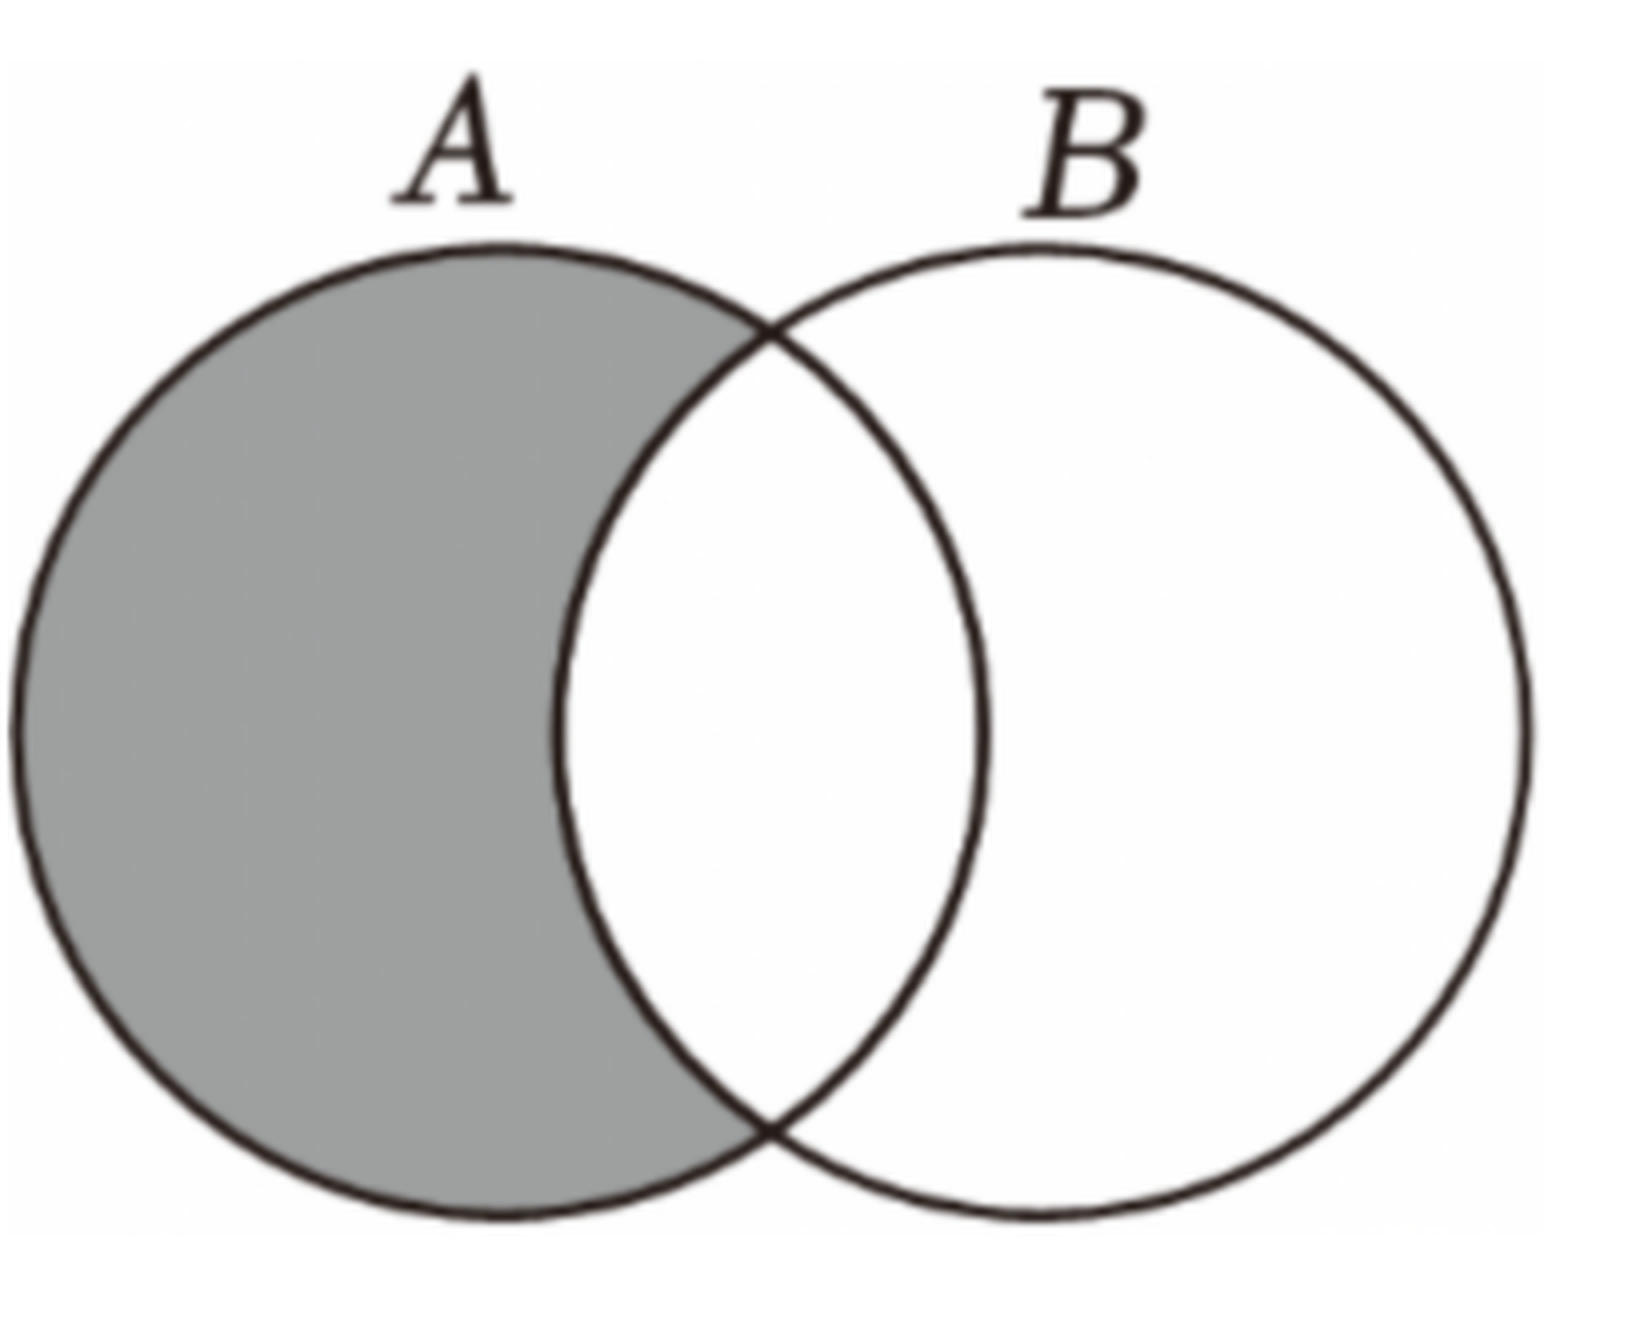
\includegraphics[width=0.30\textwidth]{figures/venn_A_minus_B_h38.png}
\end{center}

\ans{$\{1\}$}

\item 集合 $\{2,3,4,\cdots,2024,2025\}$ 的真子集的个数为 \blankline[4.4em].

\ans{$2^{2024}-1$}

\ifanswer
\solbegin
\step{集合 $\{2,3,4,\cdots,2024,2025\}$ 的真子集的个数为 $2^{2024}-1$.}
\solend

\fi

\item 已知集合 $A$ 中的元素都是正整数，其中最小的是 $1$，最大值是 $100$，除 $1$ 以外，每一个元
素都等于 $A$ 中的两个数（可以相同）的和，则集合 $A$ 中至少含有 \blankline[4.4em] 个元素.

\ans{$9$}

\ifanswer
\solbegin
\step{设 $A$ 中的数从小到大排列为 $1,a_1,a_2,\cdots,a_k,100$，}
\step{则 $a_1=1+1=2$；$3\leqslant a_2\leqslant 4$；$4\leqslant a_3\leqslant 8$；$5\leqslant a_4\leqslant 16$；$6\leqslant a_5\leqslant 32$；$7\leqslant a_6\leqslant 64$；}
\step{于是 $A$ 至少有八个数；}
\step{假设 $A$ 恰好有八个元素，由于 $a_5+a_6\leqslant 96<100$；}
\step{故必须有 $100=a_6+a_6$，$a_6=50$，}
\step{又 $a_4+a_5\leqslant 48$，同理 $a_5=25$，}
\step{但此时 $a_3+a_4\leqslant 24$，$a_5=2a_4$，$a_4=12.5$ 矛盾，}
\step{故 $A$ 不可能恰好有八个元素，因此 $A$ 至少有九个元素.}
\step{其九个数可以为 $1$，$2$，$3$，$6$，$12$，$13$，$25$，$50$，$100$.}
\solend

\fi

\item 已知集合 $\{x_1,x_2,x_3,x_4,x_5,x_6\}=\{1,2,3,4,5,6\}$，将 $x_i$ 与 $x_j$（其中 $i\in\{1,2,3\}$，
$j\in\{4,5,6\}$）的乘积 $x_ix_j$ 放入如图的 $3\times3$ 方格中，则方格中全部数之和的最大值为 \blankline[4.4em].

% 原卷的 $3\times3$ 方格是表格式内容（三行三列的公式），本稿按 高一03 的成例用 tabular 排出。
\begin{center}
\begin{tabular}{|c|c|c|}
\hline
$x_1x_4$ & $x_1x_5$ & $x_1x_6$ \\
\hline
$x_2x_4$ & $x_2x_5$ & $x_2x_6$ \\
\hline
$x_3x_4$ & $x_3x_5$ & $x_3x_6$ \\
\hline
\end{tabular}
\end{center}

\ans{$110$}

\ifanswer
\solbegin
\step{由表格数据得所有数之和为}
\step{$S=x_1x_4+x_1x_5+x_1x_6+x_2x_4+x_2x_5+x_2x_6+x_3x_4+x_3x_5+x_3x_6$，}
\step{所以 $S=(x_1+x_2+x_3)(x_4+x_5+x_6)$，}
\step{因为集合 $\{x_1,x_2,x_3,x_4,x_5,x_6\}=\{1,2,3,4,5,6\}$，}
\step{所以 $x_1+x_2+x_3+x_4+x_5+x_6=1+2+3+4+5+6=21$，}
\step{设 $t=x_1+x_2+x_3$，则 $6\leqslant t\leqslant 15$，$t\in\N^*$，}
\step{$S=t(21-t)=-\left(t-\dfrac{21}{2}\right)^2+\dfrac{441}{4}$，}
\step{当 $t=10$ 或 $t=11$ 时，$S=t(21-t)$ 取最大值，最大值为 $110$，}
\step{此时 $\{x_1,x_2,x_3\}=\{1,4,5\}$，$t=10$，所以可取最大值 $110$.}
\solend

\fi

\item 若 $[x]$ 表示不大于 $x$ 的最大整数，方程 $x^2-8[x]+7=0$ 的解集为 \blankline[4.4em].

\ans{$\{1,\sqrt{33},\sqrt{41},7\}$}

\ifanswer
\solbegin
\step{由题意，$x\geqslant[x]=\dfrac{x^2+7}{8}>0$，得 $x^2-8x+7\leqslant 0$，解得 $1\leqslant x\leqslant 7$，}
\step{$[x]=1$，$x^2=1$，$x=1$；}
\step{$[x]=2$，$x^2=9$，$x=3$ 与 $[x]=2$ 矛盾；}
\step{$[x]=3$，$x^2=17$，$x=\sqrt{17}$，$[x]=4$ 与 $[x]=3$ 矛盾；}
\step{$[x]=4$，$x^2=25$，$x=5$ 与 $[x]=4$ 矛盾；}
\step{$[x]=5$，$x^2=33$，$x=\sqrt{33}$，$[x]=5$；}
\step{$[x]=6$，$x^2=41$，$x=\sqrt{41}$，$[x]=6$；}
\step{$[x]=7$，$x^2=49$，$x=7$；}
\step{综上，方程 $x^2-8[x]+7=0$ 的解集为 $\{1,\sqrt{33},\sqrt{41},7\}$.}
\solend

\fi

\end{enumerate}

\bigsec{二、选择题}

\begin{enumerate}
\setcounter{enumi}{10}

\item 已知集合 $A=\{a,a^2\}$，$B=\{1,3\}$，若 $1\in A$，则 $A\cup B$ 中所有元素之和为\mbox{（\quad）}

\keepwithprev
A. $2$\qquad B. $3$\qquad C. $4$\qquad D. $5$

\ans{$B$}

\ifanswer
\solbegin
\step{因为 $1\in A$，集合 $A=\{a,a^2\}$，所以 $a=1$ 或 $a^2=1$，}
\step{若 $a=1$，则 $a=a^2$，与元素的互异性矛盾；}
\step{若 $a^2=1$，则 $a=1$（舍）或 $a=-1$，故 $A=\{-1,1\}$，$B=\{1,3\}$，}
\step{故 $A\cup B=\{-1,1,3\}$，所以 $A\cup B$ 中所有元素之和为 $-1+1+3=3$. 故选 $B$.}
\solend

\fi

\item 对于实数 $a$、$b$、$c$，下列命题正确的是\mbox{（\quad）}

\keepwithprev
A. 若 $a>b$，则 $ac^2>bc^2$\qquad B. 若 $a>b$，则 $a^2>b^2$

C. 若 $a>b$，则 $a|a|>b|b|$\qquad D. 若 $a>b>c>0$，则 $\dfrac{b}{a-b}<\dfrac{c}{a-c}$

\ans{$C$}

\ifanswer
\solbegin
\step{对于 $A$，若 $a>b$，$c=0$，则 $ac^2=bc^2$，故 $A$ 错误；}
\step{对于 $B$，若 $a>b$，取 $a=-1$，$b=-2$，则 $a^2<b^2$，故 $B$ 错误；}
\step{对于 $C$，若 $a>b>0$ 时，$a|a|-b|b|=a^2-b^2>0$，}
\step{当 $a>0>b$ 时，$a|a|-b|b|=a^2+b^2>0$，}
\step{当 $0>a>b$ 时，$a|a|-b|b|=b^2-a^2=(b-a)(b+a)>0$，}
\step{综上，若 $a>b$，则 $a|a|>b|b|$，故 $C$ 正确；}
\step{对于 $D$，若 $a>b>c>0$，$\dfrac{b}{a-b}-\dfrac{c}{a-c}=\dfrac{ab-bc-ac+bc}{(a-b)(a-c)}=\dfrac{a(b-c)}{(a-b)(a-c)}>0$，}
\step{故 $D$ 错误.}
\step{故选 $C$.}
\solend

\fi

\item 对于正整数集合 $A=\{a_1,a_2,\cdots,a_n\}(n\in\N^*,\ n\geqslant 3)$，如果去掉其中任意一个元素
$a_i(i=1,2,\cdots,n)$ 之后，剩余的所有元素组成的集合都能分为两个交集为空集的集合，且这
两个集合的所有元素之和相等，就称集合 $A$ 为平衡集. 记 $M=a_1+a_2+\cdots+a_n$. 若集合 $A$
是平衡集，并且存在 $a_i$ 为奇数，则集合 $A$ 中元素个数 $n$ 的奇偶性\mbox{（\quad）}

\keepwithprev
A. 与 $M$ 相关，既可以是奇数，又可以是偶数

B. 与 $M$ 无关，既可以是奇数，又可以是偶数

C. 与 $M$ 无关，必为偶数

D. 与 $M$ 无关，必为奇数

\ans{$D$}

\ifanswer
\solbegin
\step{正整数集合 $A=\{a_1,a_2,\cdots,a_n\}(n\in\N^*,\ n\geqslant 3)$，}
\step{因为集合 $A$ 是平衡集，设去掉元素 $a_i(i=1,2,\cdots,n)$，}
\step{由题意得 $A=A_1\cup A_2\cup\{a_i\}$，其中 $A_1\cap A_2=\varnothing$，}
\step{设集合 $A_1$ 和 $A_2$ 中的元素之和均为 $m$，所以 $M=2m+a_i$，其中 $i=1,2,\cdots,n$，}
\step{所以 $M-a_i=2m$，所以 $M-a_i$ 为偶数，其中 $i=1,2,\cdots,n$，}
\step{所以 $a_i(i=1,2,\cdots,n)$ 的奇偶性相同；}
\step{因为存在 $a_i$ 为奇数，所以 $a_i(i=1,2,\cdots,n)$ 均为奇数，}
\step{由 $M-a_i=2m$ 得 $M$ 也为奇数，且 $M=a_1+a_2+\cdots+a_n$，}
\step{所以 $n$ 也为奇数，所以 $n$ 必为奇数. 故选 $D$.}
\solend

\fi

\item 对于集合 $M=\{a\mid a=x^2-y^2,\ x\in\Z,\ y\in\Z\}$，给出如下三个结论：其中正确结论的个数
是\mbox{（\quad）}

\keepwithprev
①如果 $P=\{b\mid b=2n+1,\ n\in\Z\}$，那么 $P\sub M$；

②如果 $c=4n+2$，$n\in\Z$，那么 $c\notin M$；

③如果 $a_1\in M$，$a_2\in M$，那么 $a_1a_2\in M$.

\keepwithprev
A. $1$\qquad B. $2$\qquad C. $3$\qquad D. $0$

\ans{$C$}

\ifanswer
\solbegin
\step{对于①，$b=2n+1$，$n\in\Z$，则恒有 $2n+1=(n+1)^2-n^2$，}
\step{所以 $2n+1\in M$，即 $P=\{b\mid b=2n+1,n\in\Z\}$，则 $P\sub M$，①正确；}
\step{对于②，$c=4n+2$，$n\in\Z$，}
\step{若 $4n+2\in M$，则存在 $x$、$y\in\Z$ 使得 $x^2-y^2=4n+2$，}
\step{所以 $4n+2=(x+y)(x-y)$，又 $x+y$ 和 $x-y$ 同奇或同偶，}
\step{若 $x+y$ 和 $x-y$ 都是奇数，则 $(x+y)(x-y)$ 为奇数，而 $4n+2$ 是偶数；}
\step{若 $x+y$ 和 $x-y$ 都是偶数，则 $(x+y)(x-y)$ 能被 $4$ 整除，而 $4n+2$ 不能被 $4$ 整除，}
\step{所以 $4n+2\notin M$，即 $c\notin M$，②正确；}
\step{对于③，$a_1\in M$，$a_2\in M$，可设 $a_1=x_1^2-y_1^2$，$a_2=x_2^2-y_2^2$，$x_i$、$y_i\in\Z$；}
\step{则 $a_1a_2=(x_1^2-y_1^2)(x_2^2-y_2^2)=(x_1x_2)^2+(y_1y_2)^2-(x_1y_2)^2-(x_2y_1)^2$}
\step{$=(x_1x_2+y_1y_2)^2-(x_1y_2+x_2y_1)^2\in M$，那么 $a_1a_2\in M$，③正确.}
\step{综上，正确的命题是①②③. 故选 $C$.}
\solend

\fi

\end{enumerate}

\bigsec{三、解答题}

\begin{enumerate}
\setcounter{enumi}{14}

\item 已知 $A=\{x\mid a\leqslant x\leqslant -a+3\}$，$B=\{x\mid x<-1\text{ 或 }x>5\}$.

\begin{enumerate}[label=(\arabic*)]

\item 若 $A\cap B=\varnothing$，求 $a$ 的取值范围；

\item 若 $A\cup B=\R$，求 $a$ 的取值范围.

\end{enumerate}

\ans{（1）$[-1,+\infty)$；（2）$(-\infty,-2]$}

\ifanswer
\solbegin
\stepm{(1)}{①当 $A=\varnothing$ 时，$A\cap B=\varnothing$，需满足 $a>-a+3$，解得 $a>\dfrac32$，}
\step{故 $a$ 的取值范围为 $\left(\dfrac32,+\infty\right)$.}
\step{②当 $A\neq\varnothing$ 时，要使 $A\cap B=\varnothing$，需满足
$\begin{cases}a\leqslant\dfrac32\\[4pt] -a+3\leqslant 5\\[4pt] a\geqslant -1\end{cases}$，解得 $-1\leqslant a\leqslant\dfrac32$.}
\step{综上所述，$a$ 的取值范围是 $[-1,+\infty)$.}
\stepm{(2)}{因为 $A\cup B=\R$，$A=\{x\mid a\leqslant x\leqslant -a+3\}$，$B=\{x\mid x<-1\text{ 或 }x>5\}$，}
\step{所以 $\begin{cases}-a+3\geqslant 5\\[4pt] a\leqslant -1\end{cases}$，解得 $a\leqslant -2$，故所求 $a$ 的取值范围为 $(-\infty,-2]$.}
\solend

\fi

\ansspace[6]

\item 已知集合 $A=\{x\mid mx^2+x-2=0\}$，$B=\{x\mid 2x^2-5x-12=0\}$.

\begin{enumerate}[label=(\arabic*)]

\item 若 $A$ 中有且仅有 $1$ 个元素，求实数 $m$ 的值；

\item 已知集合 $C=A\cup B$，若 $C$ 的真子集有且仅有 $3$ 个，求实数 $m$ 的取值范围.

\end{enumerate}

\ans{（1）$m=0$ 或 $m=-\dfrac18$；（2）$\left\{m\mid m\leqslant -\dfrac18\right\}$}

\ifanswer
\solbegin
\stepm{(1)}{若 $m=0$，方程化为 $x-2=0$，此时方程有且仅有一个根 $x=2$；}
\step{若 $m\neq 0$，则 $\Delta=1^2-4\times m\times(-2)=0$，即 $m=-\dfrac18$ 时，}
\step{方程有两个相等的实根，此时集合 $A$ 中有且仅有一个元素，}
\step{所以实数 $m$ 的值为 $m=0$ 或 $m=-\dfrac18$；}
\stepm{(2)}{$B=\{x\mid 2x^2-5x-12=0\}=\left\{-\dfrac32,4\right\}$，}
\step{因为 $C=A\cup B$，若 $C$ 的真子集有且仅有 $3$ 个，则 $C$ 中有两个元素，}
\step{所以 $A\sub B$，由（1）得 $m=0$ 时，$A=\{2\}$，不符合 $A\sub B$，}
\step{当 $m\neq 0$ 时，若 $\Delta=1^2-4\times m\times(-2)<0$，解得 $m<-\dfrac18$，}
\step{此时 $A=\varnothing$，符合 $A\sub B$，}
\step{若 $\Delta=1^2-4\times m\times(-2)=0$，解得 $m=-\dfrac18$，}
\step{此时方程 $mx^2+x-2=0$ 的根为 $x=4$，集合 $A=\{4\}$，符合 $A\sub B$，}
\step{若 $\Delta=1^2-4\times m\times(-2)>0$，由 $A\sub B$，得 $A=\left\{-\dfrac32,4\right\}$，}
\step{此时有 $-\dfrac32+4=-\dfrac1m$ 且 $-\dfrac32\times 4=-\dfrac2m$，无解，}
\step{综上所述，实数 $m$ 的取值范围为 $\left\{m\mid m\leqslant -\dfrac18\right\}$.}
\solend

\fi

\ansspace[6]

\item 设 $A$ 是非空实数集，且 $0\notin A$. 若对于任意的 $x$、$y\in A$，都有 $xy\in A$，则称集合 $A$ 具
有性质 $P_1$；若对于任意的 $x$、$y\in A$，都有 $\dfrac xy\in A$，则称集合 $A$ 具有性质 $P_2$.

\begin{enumerate}[label=(\arabic*)]

\item 写出一个恰含有两个元素且具有性质 $P_1$ 的集合 $A$，并说明理由；

\item 证明：“非空实数集 $A$ 具有性质 $P_1$”是“非空实数集 $A$ 具有性质 $P_2$”的必要非充分条
件.

\end{enumerate}

\ans{（1）$A=\{-1,1\}$，理由见解析；（2）见解析}

\ifanswer
\solbegin
% 注：原卷本题 (1) 的解析里“证明”一词重复出现两次（一次接在分号后、一次另起一行），
%     本稿照原卷重复录入，未去重。
\stepm{(1)}{$A=\{-1,1\}$，证明：恰含有两个元素且具有性质 $P_1$ 的集合 $A=\{-1,1\}$；}
\step{证明：$1\times 1=1\in A$，$1\times(-1)=-1\in A$，$-1\times 1=-1\in A$，$-1\times(-1)=1\in A$；}
\stepm{(2)}{若集合 $A$ 具有性质 $P_2$，不妨设 $a\in A$，}
\step{由非空数集 $A$ 具有性质 $P_2$，有 $\dfrac aa=1\in A$.}
\step{①$A=\{1\}$，易得此时集合 $A$ 具有性质 $P_1$.}
\step{②数集 $A$ 只含有两个元素，不妨设 $A=\{1,a_1\}$，}
\step{由 $\dfrac{1}{a_1}=a_1$，且 $a_1\neq 1$，解得 $a_1=-1$，此时集合 $A$ 具有性质 $P_1$.}
\step{③实数集 $A$ 含有两个以上的元素，不妨设不为 $1$ 的元素 $a_1$、$a_2\in A$，}
\step{则有 $\dfrac{1}{a_1}\in A$，由于集合 $A$ 具有性质 $P_2$，}
\step{所以有 $a_2\div\dfrac{1}{a_1}=a_1a_2\in A$，这说明集合 $A$ 具有性质 $P_1$.}
\step{综上，若非空实数集 $A$ 具有性质 $P_2$，则集合 $A$ 具有性质 $P_1$，}
\step{所以“非空实数集 $A$ 具有性质 $P_1$”是“非空实数集 $A$ 具有性质 $P_2$”的}
\step{必要条件.}
\step{取正偶数集 $A=\{x\mid x=2n,\ n\in\N^*\}$，}
\step{对任意的 $2m$、$2n\in A$，$m$、$n\in\N^*$，}
\step{有 $2m\times 2n=4mn\in A$，故 $A$ 具有性质 $P_1$，}
\step{取 $x=2$，$y=4$，则 $\dfrac xy=\dfrac12\notin A$，故 $A$ 不具有性质 $P_2$，}
\step{所以“非空实数集 $A$ 具有性质 $P_1$”不是“非空实数集 $A$ 具有性质 $P_2$”的}
\step{充分条件.}
\step{综上，“非空实数集 $A$ 具有性质 $P_1$”是“非空实数集 $A$ 具有性质 $P_2$”的}
\step{必要非充分条件.}
\solend

\fi

\ansspace[8]

\item 已知命题 $p$：关于 $x$ 的方程 $x^2+mx+1=0$ 有两个不同的正根；命题 $q$：关于 $x$ 的方程
$4x^2+4(m-2)x=-1$ 有实根.

\begin{enumerate}[label=(\arabic*)]

\item 若命题 $q$ 为假命题，求整数 $m$ 的解集；

\item 若命题 $p$ 为真命题，且关于 $x$ 的方程 $x^2+mx+1=0$ 的两个实数根 $x_1$、$x_2$ 满足
$3x_1+2x_2=5$，求实数 $m$ 的取值集合；

\item 若命题 $p$ 和命题 $q$ 有且仅有一个成立，求实数 $m$ 的取值范围.

\end{enumerate}

\ans{（1）$\{2\}$；（2）$\left\{-\dfrac{13}{6}\right\}$；（3）$[-2,1]\cup[3,+\infty)$}

\ifanswer
\solbegin
\stepm{(1)}{命题 $q$：关于 $x$ 的方程 $4x^2+4(m-2)x=-1$ 有实根为假命题，}
\step{即 $4x^2+4(m-2)x+1=0$ 无实根，}
\step{则 $\Delta=16(m-2)^2-16<0$，则 $1<m<3$，则整数 $m$ 的解集为 $\{2\}$；}
\stepm{(2)}{若命题 $p$ 为真命题，且关于 $x$ 的方程 $x^2+mx+1=0$ 的两个实数根 $x_1$、$x_2$，}
\step{满足 $3x_1+2x_2=5$，则方程 $x^2+mx+1=0$ 有两个不同的正根，}
\step{则 $\begin{cases}\Delta=m^2-4>0\\[4pt] x_1+x_2=-m>0\end{cases}$，则 $m<-2$，}
\step{又 $\begin{cases}x_1+x_2=-m\\[4pt] x_1x_2=1\\[4pt] 3x_1+2x_2=5\end{cases}$，
则 $\begin{cases}x_1=5+2m\\[4pt] x_2=-3m-5\end{cases}$，则 $(5+2m)(-3m-5)=1$，}
\step{得 $m=-2$ 或 $m=-\dfrac{13}{6}$，又因为 $m<-2$，所以 $m=-\dfrac{13}{6}$，}
\step{所以实数 $m$ 的取值集合为 $\left\{-\dfrac{13}{6}\right\}$；}
\stepm{(3)}{由（2）得当 $p$ 为真时，则有 $m<-2$，}
\step{当 $q$ 为真时，$\Delta=16(m-2)^2-16\geqslant 0$，解得 $m\leqslant 1$ 或 $m\geqslant 3$，}
\step{又因为命题 $p$ 和命题 $q$ 只有一个为真，所以
$\begin{cases}m<-2\\[4pt] 1<m<3\end{cases}$ 或 $\begin{cases}m\geqslant -2\\[4pt] m\leqslant 1\text{ 或 }m\geqslant 3\end{cases}$，}
\step{解得 $-2\leqslant m\leqslant 1$ 或 $m\geqslant 3$，所以实数 $m$ 的取值范围为 $[-2,1]\cup[3,+\infty)$.}
\solend

\fi

\ansspace[8]

% 注：原卷此处作“设 $n\in\N^*$，集合含有 $3n$ 个元素”，**漏了符号 $U$**（应作“集合 $U$
%     含有 $3n$ 个元素”）——$U$ 直到本句末尾“则称 $U$ 为三分集合”才出现、此前无定义。
%     本稿照录未补，见文件头“原卷笔误/存疑”⑦。
\item 设 $n\in\N^*$，集合含有 $3n$ 个元素，若存在三个 $n$ 元集合 $A$、$B$、$C$ 满足如下两个条件，
则称 $U$ 为三分集合.

①$U=A\cup B\cup C$；

②$A$、$B$、$C$ 元素可分别排列为有序数组 $(a_1,a_2,\cdots,a_n)$，$(b_1,b_2,\cdots,b_n)$ 及
$(c_1,c_2,\cdots,c_n)$，使得对 $\forall i=1,2,\cdots,n$，均有 $a_i+b_i=c_i$.

特别地，当 $U=\{1,2,3,4,\cdots,3n-2,3n-1,3n\}$ 为三分集合时，称 $n$ 为完美三分数.

如：因为 $U=\{1,2,3\}$ 为三分集合，所以 $n=1$ 为最小完美三分数.

\begin{enumerate}[label=(\arabic*)]

\item 请判断下列两个集合是否为三分集合（直接写出结论）：

$U_1=\{1,2,3,4,5,6\}$，$U_2=\{1,3,5,7,8,9,10,11,12\}$；

\item 求出大于 $1$ 的最小完美三分数；

\item 请判断是否存在无穷多个完美三分数？若存在，请说明理由；若不存在，则求出最大的
完美三分数.

\end{enumerate}

\ans{（1）$U_1$ 不是三分集合，$U_2$ 是三分集合；（2）$4$；（3）存在，理由见解析}

\ifanswer
\solbegin
\stepm{(1)}{(i)$U_1=\{1,2,3,4,5,6\}$ 不是三分集合，下面用反证法证明：}
\step{证明：假设 $U=\{1,2,3,4,5,6\}$ 是三分集合，}
\step{设 $A=\{a_1,a_2\}$，$B=\{b_1,b_2\}$，$C=\{c_1,c_2\}$，不妨设 $c_1<c_2$，}
\step{因为 $a_1+b_1=c_1$，$a_2+b_2=c_2$，}
\step{所以 $a_1+b_1+a_2+b_2+c_1+c_2=2(c_1+c_2)=1+2+3+4+5+6=21$，}
% 注：原卷此步印“所以 $c_1+c_2=2$”，与上一行的 $2(c_1+c_2)=21$ **不自洽**
%     （应作 $\dfrac{21}2$）；同题 $n=3$ 处的同型推理原卷写的是 $\dfrac{45}2$，故此处是原卷笔误。
%     本稿照录未改，见文件头“原卷笔误/存疑”⑧。
\step{所以 $c_1+c_2=2$，这与 $c_1,c_2\in\N^*$ 矛盾，故假设错误，}
\step{故 $U_1=\{1,2,3,4,5,6\}$ 不是三分集合；}
\step{(ii)$U_2=\{1,3,5,7,8,9,10,11,12\}$ 是三分集合，理由如下：}
\step{令 $A=\{1,3,5\}$，$B=\{9,8,7\}$，$C=\{10,11,12\}$，}
\step{则 $A\cup B\cup C=U=\{1,3,5,7,8,9,10,11,12\}$，满足条件①；}
\step{又 $1+9=10$；$3+8=11$；$5+7=12$，所以满足条件②，}
\step{所以 $U_2=\{1,3,5,7,8,9,10,11,12\}$ 是三分集合；}
\stepm{(2)}{由（1）得，当 $n=2$ 时，$U=\{1,2,3,4,5,6\}$ 不是三分集合；}
\step{当 $n=3$ 时，$U=\{1,2,3,4,5,6,7,8,9\}$，}
\step{假设 $U=\{1,2,3,4,5,6,7,8,9\}$ 是三分集合，}
\step{同理由 $a_1+b_1+a_2+b_2+a_3+b_3+c_1+c_2+c_3$}
\step{$=2(c_1+c_2+c_3)=1+2+\cdots+9=45$，$c_1+c_2+c_3=\dfrac{45}{2}$，}
\step{可推出与 $c_1$、$c_2$、$c_3\in\N^*$ 矛盾，故假设也错误，}
\step{所以 $U=\{1,2,3,4,5,6,7,8,9\}$ 不是三分集合；}
\step{当 $n=4$ 时，$U=\{1,2,3,\cdots,12\}$，}
\step{存在三个 $4$ 元集合 $A=\{1,2,4,3\}$，$B=\{5,8,7,9\}$，$C=\{6,10,11,12\}$，}
\step{满足 $U=\{1,2,3,\cdots,12\}$ 为三分集合的两个条件，}
\step{故大于 $1$ 的最小完美三分数为 $4$；}
\stepm{(3)}{存在无穷多个完美三分数，理由如下：}
\step{由题意得，$n=1$ 为最小完美三分数，}
\step{当 $n=5$ 时，$U=\{1,2,3,\cdots,15\}$，}
\step{存在三个 $5$ 元集合 $A=\{1,3,5,7,2\}$，$B=\{11,10,9,8,4\}$，$C=\{12,13,14,15,6\}$，}
\step{满足三分集合的条件，故 $5$ 为完美三分数；}
\step{当 $n=21$ 时，$U=\{1,2,3,\cdots,63\}$，}
\step{存在如下三个 $21$ 元的集合满足三分集合的条件：}
\step{$A=\{1,3,5,7,\cdots,29,31,2,6,10,14,4\}$，}
\step{$B=\{47,46,45,44,\cdots,33,32,22,20,18,16,8\}$，}
\step{$C=\{48,49,50,51,\cdots,62,63,24,26,28,30,12\}$，}
\step{故 $21$ 为完美三分数.}
\step{首先证明：若 $n=k$，$k\in\N^*$ 为三分完美数，}
\step{则 $n=4k+1$，$k\in\N^*$ 也为三分完美数，}
% 注：下一行原卷印作“$U_{k+1}=U_{k+1}=\{2,3,\cdots,12k+3\}$”——等号两边记号相同，
%     依上下文疑当作 $U'_{k+1}=U_{4k+1}$，且此处集合自 2 起（前文 $U_{4k+1}$ 自 1 起）；
%     本稿照录原卷，未代为改写。
\step{证明：记 $U_k=\{1,2,3,\cdots,3k\}$，$U_{4k+1}=\{1,2,3,\cdots,12k+3\}$，}
\step{若 $n=k$，$k\in\N^*$ 为三分完美数，则 $U_k$ 为三分集合，}
\step{即存在三个 $k$ 元集合 $A$、$B$、$C$ 满足如下两个条件，}
\step{①$U_k=A\cup B\cup C$；}
\step{②$A$、$B$、$C$ 元素可分别排列为有序数组 $(a_1,a_2,\cdots,a_k)$，}
\step{$(b_1,b_2,\cdots,b_k)$ 及 $(c_1,c_2,\cdots,c_k)$，}
\step{使得对 $\forall i=1,2,3,\cdots,k$，均有 $a_i+b_i=c_i$，}
\step{则可得到对 $\forall i=1,2,3,\cdots,k$，$2a_i+2b_i=2c_i$，}
\step{故集合 $\{2,4,6,\cdots,6k\}$ 也满足三分集合的两个条件，其也为三分集合，}
\step{下面记集合 $\{2,4,6,\cdots,6k\}=2U_k$，}
\step{对 $n=4k+1$，集合 $U_{k+1}=U_{k+1}=\{2,3,\cdots,12k+3\}=(2U_k)\cup\complement_{U_{4k+1}}(2U_k)$，}
\step{构造集合 $A'=\{1,3,5,7,\cdots,6k+1\}$，共有 $3k+1$ 个奇数；}
% 注：下一行原卷印作“$B'=\{6k+3k+2,6k+3k+1,6k+3k,6k+3k-1,\cdots,6k+2\}$”，
%     按与后文 $C'$ 相接，前四项当写作 $9k+2$、$9k+1$、$9k$、$9k-1$；本稿照录原卷。
\step{集合 $B'=\{6k+3k+2,6k+3k+1,6k+3k,6k+3k-1,\cdots,6k+2\}$，}
\step{共有 $3k+1$ 个逐个减小的连续正整数；}
\step{集合 $C'=\{9k+3,9k+4,9k+5,9k+6,\cdots,12k+3\}$，}
\step{共有 $3k+1$ 个逐个增大的连续正整数；}
\step{得这三个 $3k+1$ 元集合 $A'$、$B'$、$C'$ 满足如下两个条件，}
\step{①集合 $A'\cup B'\cup C'=\complement_{U_{4k+1}}(2U_k)$；}
\step{②$A'$、$B'$、$C'$ 元素可分别排列为有序数组 $(a_1,a_2,\cdots,a_{3k+1})$，}
\step{$(b_1,b_2,\cdots,b_{3k+1})$ 及 $(c_1,c_2,\cdots,c_{3k+1})$，}
\step{使得对 $\forall i=1,2,3,\cdots,3k+1$，均有 $a_i+b_i=c_i$；}
\step{故 $\complement_{U_{4k+1}}(2U_k)$ 为三分集合，而已知 $U_k$ 为三分集合，}
\step{将其对应与 $A'$、$B'$、$C'$ 合并，}
% 注：原卷此处印“令 $A''=A\cup A'$”（$B''$、$C''$ 同）。按同段上文“记集合
%     $\{2,4,6,\cdots,6k\}=2U_k$”，此处疑当作 $A''=2A\cup A'$——否则
%     $A''\cup B''\cup C''=U_k\cup\complement_{U_{4k+1}}(2U_k)\neq U_{4k+1}$，与本段结论冲突。
%     本稿照录未改，见文件头“原卷笔误/存疑”⑨。
\step{令 $A''=A\cup A'$，$B''=B\cup B'$，$C''=C\cup C'$，}
\step{则这三个 $4k+1$ 元集合 $A''$、$B''$、$C''$，}
\step{满足 $A''\cup B''\cup C''=U_{4k+1}$，且满足条件②，}
\step{故 $U_{4k+1}=\{1,2,3,\cdots,12k+3\}$ 为三分集合，}
\step{因此可得，若 $n=k$ 为三分完美数，则 $n=4k+1$ 也为三分完美数，}
\step{由 $1$，$5$，$21$ 为完美三分数，结合所证结论得，存在无穷多个完美三分数.}
\solend

\fi

\ansspace*[12]

\end{enumerate}

\end{document}
"
%
% 原始材料是微信公众号图文（公众号“魔都数学加油站”连载“27学年高一 38”，署名“破晓”，
% 2026-09-26 21:29 发布，原文标题“27学年高一38——2026-2027年上海市大同中学高一上周末作业3”，
% 原文链接 https://mp.weixin.qq.com/s/O_O60vCIiGi2xponAo4irw ），正文为 12 张 PNG 页。
% **同一篇里各页分辨率不一致**（2560×3620 与 4762×6735 两档混排：第 1、10、11、12 页为
% 2560×3620，第 2—9 页为 4762×6735）。原文本身就是一份**讲评版**——有的题下方只印
% 【答案】行，有的只印【解析】。试题文字、答案与解析均照原卷录入，未改内容。卷面的粉色
% 斜水印“魔都数学加油站”属水印，未录入。
%
% 本卷共 **17 题**：填空题 8 题（第 3—10 题）、选择题 4 题（第 11—14 题）、解答题 5 题
% （第 15—19 题）；插图 1 张（第 6 题 Venn 图）。三版页数：试卷版 4 页 / 答案版 11 页 /
% 紧凑版 3 页，`Overfull`／`Underfull`／`Missing character` 告警均为 0。
%
% 卷首标题：原卷印作“2026-2027 年大同中学高一上周末作业 3”（公众号原文标题里的“上海市”
% 三字卷面标题行没有，本稿照卷面），年份区间按全稿惯例排 en dash，前缀照原卷保留“年”。
%
% 与原卷的排版差异（均已在 README“说明”中交代）：
%   ① 原文自**第 3 题**起（第 1、2 题未在该文中发布），故本稿题号亦自 3 起，填空题以
%      \setcounter{enumi}{2} 起编；选择、解答两节各按上一节末号另设 \setcounter
%      （选择题 \setcounter{enumi}{10}、解答题 \setcounter{enumi}{14}）；
%   ② 原卷本就印有“一、填空题”“二、选择题”“三、解答题”三节标题，本稿照原卷分节，
%      只把标题改排成全稿统一的“大节标题”样式；
%   ③ 原卷是“讲评版”：第 3、6 题只印【答案】行，第 4、5、7、8、9、10 题与第 11—19 题印
%      【解析】；本稿统一改为试卷版隐去、答案版以 \ans{}／\ifanswer 块给出，两版彻底分离。
%      其中第 4、5、7、8、9、10 题与第 11—14 题的答案，原卷写在【解析】末句，本稿另提为
%      \ans{}；第 15—19 题原卷只有【解析】、无独立答案行，本稿亦补了摘要式 \ans{}。
%      **故本卷 17 题每题都有 \ans**——比“只印【解析】的填空、解答题不另提 \ans”的
%      高一31／高一34 更彻底，与 高一21 第 11 题（填空，答案在【解析】末句，本稿另提）同类；
%      （本仓对“另提 \ans{}”的做法各卷不一，见 README 对应专记的核对面。）
%   ④ 数集记号原卷两套并用：第 3、5 题的实数集作粗体 $\mathbf{R}$，第 8、14、17、18 题等的
%      整数集、自然数集作斜体 $Z$、$N$，本稿按全稿惯例统一写作 $\R$、$\Z$、$\N$；
%   ⑤ 原卷填空的横线宽度不一（约 1.8—3.6 字宽），本稿按全稿惯例统一排 \blankline[4.4em]；
%   ⑥ 中文括注原卷用半角“(  )”，本稿按全稿惯例排全角；选择题的作答括注统一排
%      \mbox{（\quad）}（第 14 题的作答括注原卷印在 ①②③ 三个命题**之前**，本稿照原卷次序）；
%      数学式内部的括注（如第 4 题的 $p\%(0<p<100)$、第 13 题的 $a_i(i=1,2,\cdots,n)$）照原样
%      留在行内公式里，未改全角；
%   ⑦ 原卷并列的字母（“x,y”“a,b,c”）不加标点或作半角逗号，本稿按全稿惯例改排顿号；
%   ⑧ 第 6 题的 Venn 图取原卷截图、4× LANCZOS 放大（figures/venn_A_minus_B_h38.png，
%      见该处 \includegraphics 前的注释）；第 9 题的 $3\times3$ 方格属**表格式**内容，
%      本稿按 高一03 的成例用 tabular 排出，未截图；
%   ⑨ 原卷未印副标题，本稿按**本卷实际内容**补出副标题“集合与常用逻辑用语”（依据见下条）；
%   ⑩ 原卷【解析】**一个印刷行照录为一条 `\step`**（原卷的折行也照录为独立一条，如第 17 题
%      末三处“…的”／“必要条件.”这类跨行句、第 9 题“由表格数据得所有数之和为”／
%      “$S=\cdots$，”），使答案版的排布与原卷讲评版逐行对应；全卷 15 处【解析】合计
%      **191 条 `\step` ＝ 原卷 191 行**（逐处：5、5、1、9、9、9、4、9、9、12、6、14、21、13、65）。
%
% 副标题（\examtitlest 第二个参数）：本卷卷面未印副标题，由本稿补出，取值按 2026-09-26 起的
%   新口径“只用本卷实际内容的模块名”定为“集合与常用逻辑用语”。依据：全卷 17 题
%   （第 3—19 题）中，第 3、5、6、7、8、9、10、11、13、14、15、16、17、18、19 题共 15 题
%   是集合的运算与关系、子集计数、集合新定义（性质 $P_1$／$P_2$、平衡集、三分集合），以及
%   命题与逻辑（第 3 题即用反证法证明“$x+y>2\Rightarrow x>1$ 或 $y>1$”这一命题）；不等式只
%   出现在第 4 题（降价提价的应用比较）、第 12 题（不等式命题真假）与第 10 题解析里解一元
%   二次不等式，合计不足全卷的三分之一，故不并标“不等式”。
%
% 原卷笔误/存疑（均照抄原卷、未改，见源码中该处上方注释）：
%   ① 第 19 题 (3) 的证明里印作“集合 $U_{k+1}=U_{k+1}=\{2,3,\cdots,12k+3\}$”——等号两边
%      记号相同（依上下文疑当作 $U'_{k+1}=U_{4k+1}$），且此处集合自 $2$ 起，而前文
%      $U_{4k+1}=\{1,2,3,\cdots,12k+3\}$ 自 $1$ 起；本稿照录；
%   ② 第 19 题 (3) 的证明里印作
%      “$B'=\{6k+3k+2,6k+3k+1,6k+3k,6k+3k-1,\cdots,6k+2\}$”——按与后文
%      $C'=\{9k+3,9k+4,9k+5,9k+6,\cdots,12k+3\}$ 相接，前四项当写作 $9k+2$、$9k+1$、
%      $9k$、$9k-1$（即 $6k+3k+2$ 等），原卷即作“$6k+3k+\cdots$”形式，本稿照录；
%   ③ 第 19 题的术语前后不一：题干与 (1)(2)(3) 用“完美三分数”，而 (3) 的证明里五次写作
%      “三分完美数”（词序不同）；本稿五处都照录；
%   ④ 第 14 题题干作“给出如下三个结论：其中正确结论的个数是（\quad）”，此处冒号疑当作
%      逗号，本稿照录；
%   ⑤ 第 17 题题干作“非空实数集”，其解析有一处写作“非空数集”；本稿照录；
%   ⑥ 第 17 题 (1) 的【解析】原卷连写“…集合 $A=\{-1,1\}$；证明：…；证明：…”，“证明”
%      一词重复出现两次（第一次在分行处、第二次另起一行），本稿照原卷重复录入，未去重。
%   ⑦ 第 19 题**题干漏字**：原卷作“19.设 $n\in\N^*$，集合含有 $3n$ 个元素…则称 $U$ 为
%      三分集合”——首句漏了符号 $U$（应作“集合 $U$ 含有 $3n$ 个元素”），$U$ 直到结论句
%      才出现、此前无定义；本稿照录未补（见该处上方注释）。
%   ⑧ 第 19(1)(i) 的【解析】**自相矛盾**：上一行印“$a_1+b_1+a_2+b_2+c_1+c_2=2(c_1+c_2)
%      =1+2+3+4+5+6=21$”，下一行却印“所以 $c_1+c_2=2$”（由 $2(c_1+c_2)=21$ 应得
%      $c_1+c_2=\dfrac{21}2$，非整数、才与 $c_1,c_2\in\N^*$ 矛盾）；同题 $n=3$ 处的同型
%      推理原卷就写对了（$\dfrac{45}2$），故此处是原卷笔误；本稿照录未改（见该处上方注释）。
%   ⑨ 第 19(3) 的【解析】印“令 $A''=A\cup A'$，$B''=B\cup B'$，$C''=C\cup C'$”——按同段
%      上文“记集合 $\{2,4,6,\cdots,6k\}=2U_k$”，$A''$ 等疑当作 $2A\cup A'$（$B''$、$C''$ 同），
%      否则 $A''\cup B''\cup C''=U_k\cup\complement_{U_{4k+1}}(2U_k)\neq U_{4k+1}$；本稿照录未改
%      （见该处上方注释）。

\documentclass[a4paper,11pt]{article}
\usepackage{common}

\begin{document}

\examtitlest[3]{2026--2027 年大同中学高一上周末作业 3}{集合与常用逻辑用语}

\bigsec{一、填空题}

\begin{enumerate}
% 原卷填空题自第 3 题起（第 1、2 题未在该文中发布），须与选择、解答两节的 \setcounter 对齐
\setcounter{enumi}{2}

\item 设 $x$、$y\in\R$，若 $x+y>2$，则 $x>1$ 或 $y>1$ 是真命题. 这个命题可以用反证法去证明，
可以假设：\blankline[4.4em].

\ans{$x\leqslant 1$ 且 $y\leqslant 1$}

\item 已知某商品的原价为 $a$ 元，由于市场原因，先降价 $p\%(0<p<100)$ 出售，一段时间后，
再提价 $p\%$ 出售，则该商品提价后的售价 \blankline[4.4em] 该商品的原价（填“高于”“低于”或“等于”）.

\ans{低于}

\ifanswer
\solbegin
\step{由题意得第一次降价后的售价为 $a(1-p\%)$ 元，}
\step{第二次提价后的售价为 $a(1-p\%)(1+p\%)$ 元，}
\step{因为 $0<p<100$，所以 $0<p\%<1$，}
\step{因为 $a(1-p\%)(1+p\%)=a[1-(p\%)^2]<a$，}
\step{即该商品提价后的售价低于该商品的原价.}
\solend

\fi

\item 若集合 $A=\{x\mid ax^2+ax+1=0,\ a\in\R,\ x\in\R\}$ 的子集只有两个，则实数 $a=$ \blankline[4.4em].

\ans{$4$}

\ifanswer
\solbegin
\step{集合 $A=\{x\mid ax^2+ax+1=0\}$ 的子集只有两个，}
\step{所以 $A$ 有且只有一个元素，}
\step{①若 $a=0$，则 $A=\varnothing$ 不成立；}
\step{②若 $a\neq 0$，则 $\Delta=a^2-4a=0$，解得 $a=4$（$0$ 舍）.}
\step{故 $a=4$.}
\solend

\fi

\item 如图，已知集合 $A=\{1,2,3,4,5\}$，集合 $B=\{2,3,4,5,9\}$，则图中阴影部分所表示的
集合为 \blankline[4.4em].

% 图取原卷截图（01.png，2560×3620）右栏，4× LANCZOS 放大；为避免与 高一11 的
% figures/venn_A_minus_B.png 同名，按 高一32 的成例加 _h38 后缀。
\begin{center}
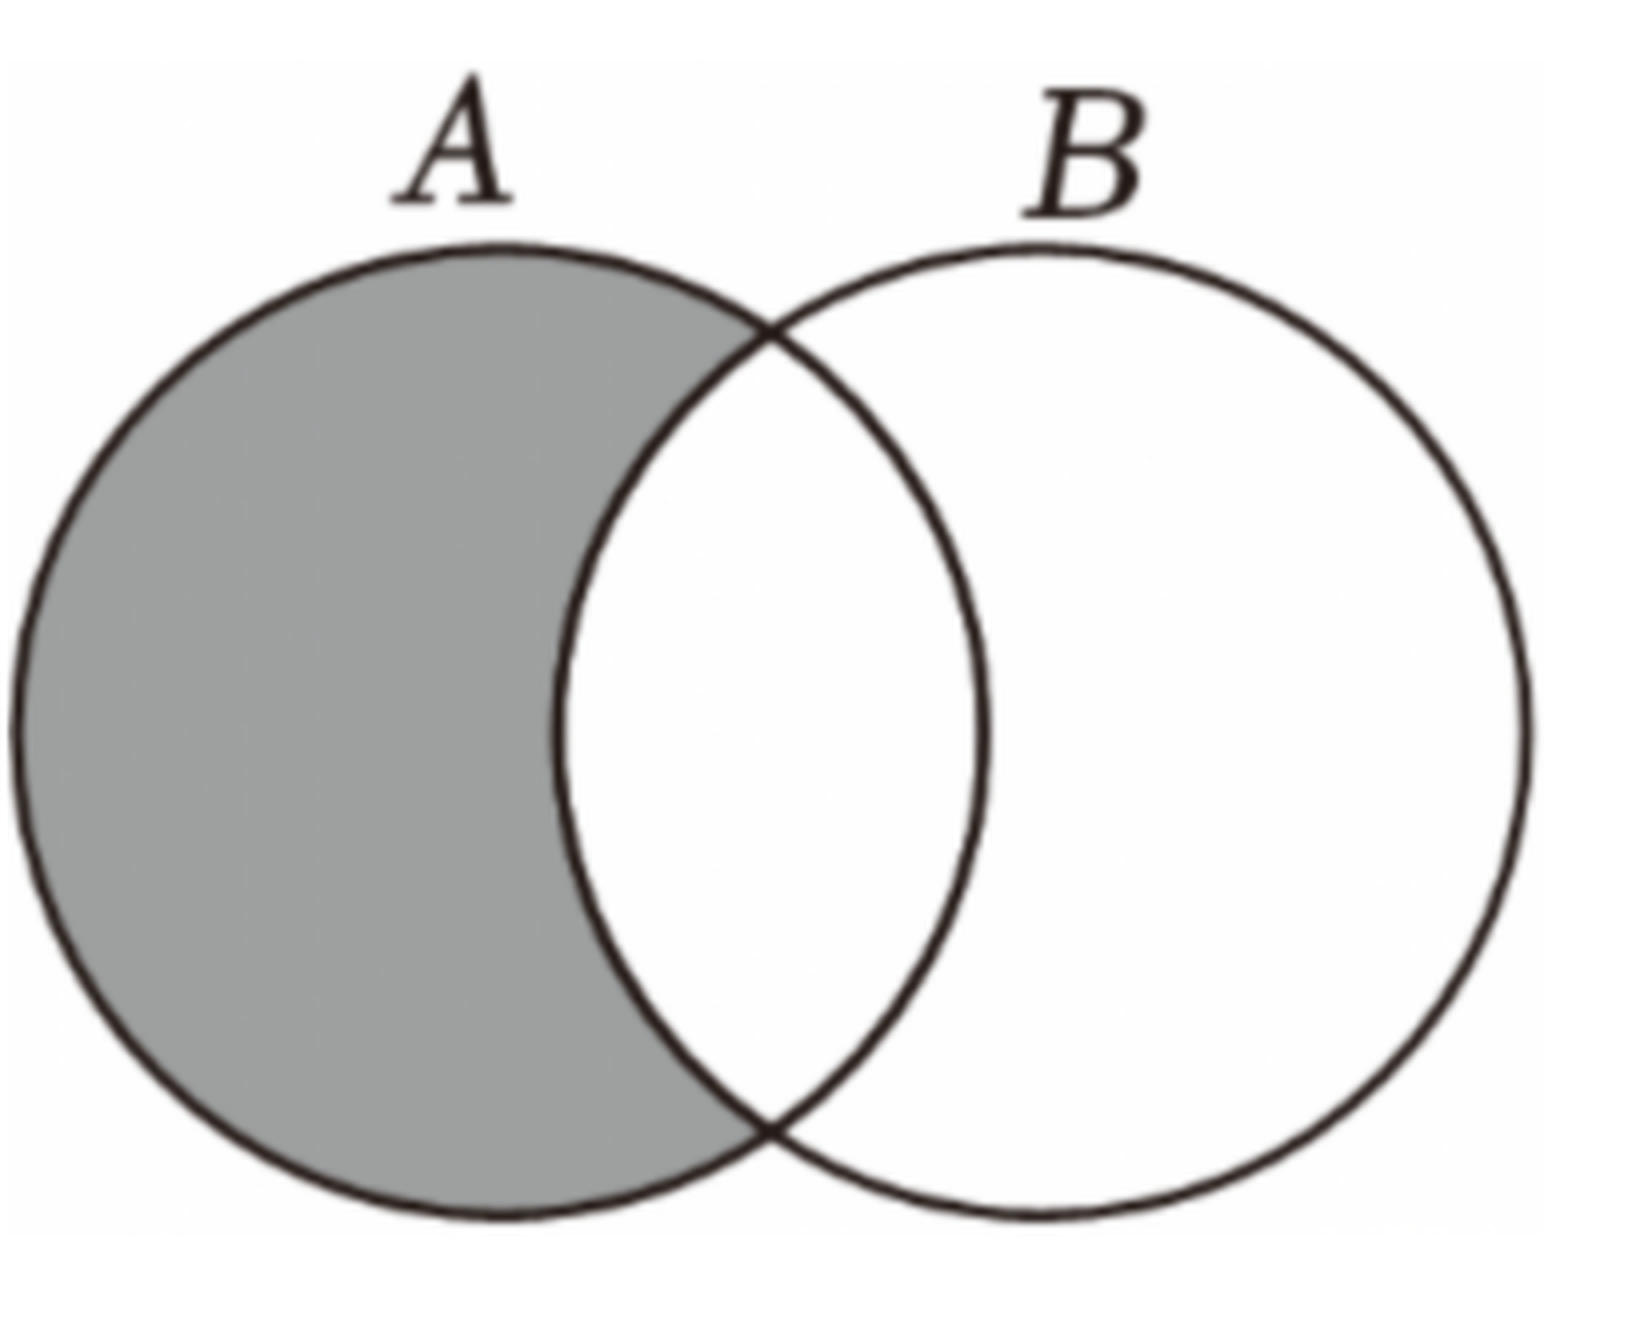
\includegraphics[width=0.30\textwidth]{figures/venn_A_minus_B_h38.png}
\end{center}

\ans{$\{1\}$}

\item 集合 $\{2,3,4,\cdots,2024,2025\}$ 的真子集的个数为 \blankline[4.4em].

\ans{$2^{2024}-1$}

\ifanswer
\solbegin
\step{集合 $\{2,3,4,\cdots,2024,2025\}$ 的真子集的个数为 $2^{2024}-1$.}
\solend

\fi

\item 已知集合 $A$ 中的元素都是正整数，其中最小的是 $1$，最大值是 $100$，除 $1$ 以外，每一个元
素都等于 $A$ 中的两个数（可以相同）的和，则集合 $A$ 中至少含有 \blankline[4.4em] 个元素.

\ans{$9$}

\ifanswer
\solbegin
\step{设 $A$ 中的数从小到大排列为 $1,a_1,a_2,\cdots,a_k,100$，}
\step{则 $a_1=1+1=2$；$3\leqslant a_2\leqslant 4$；$4\leqslant a_3\leqslant 8$；$5\leqslant a_4\leqslant 16$；$6\leqslant a_5\leqslant 32$；$7\leqslant a_6\leqslant 64$；}
\step{于是 $A$ 至少有八个数；}
\step{假设 $A$ 恰好有八个元素，由于 $a_5+a_6\leqslant 96<100$；}
\step{故必须有 $100=a_6+a_6$，$a_6=50$，}
\step{又 $a_4+a_5\leqslant 48$，同理 $a_5=25$，}
\step{但此时 $a_3+a_4\leqslant 24$，$a_5=2a_4$，$a_4=12.5$ 矛盾，}
\step{故 $A$ 不可能恰好有八个元素，因此 $A$ 至少有九个元素.}
\step{其九个数可以为 $1$，$2$，$3$，$6$，$12$，$13$，$25$，$50$，$100$.}
\solend

\fi

\item 已知集合 $\{x_1,x_2,x_3,x_4,x_5,x_6\}=\{1,2,3,4,5,6\}$，将 $x_i$ 与 $x_j$（其中 $i\in\{1,2,3\}$，
$j\in\{4,5,6\}$）的乘积 $x_ix_j$ 放入如图的 $3\times3$ 方格中，则方格中全部数之和的最大值为 \blankline[4.4em].

% 原卷的 $3\times3$ 方格是表格式内容（三行三列的公式），本稿按 高一03 的成例用 tabular 排出。
\begin{center}
\begin{tabular}{|c|c|c|}
\hline
$x_1x_4$ & $x_1x_5$ & $x_1x_6$ \\
\hline
$x_2x_4$ & $x_2x_5$ & $x_2x_6$ \\
\hline
$x_3x_4$ & $x_3x_5$ & $x_3x_6$ \\
\hline
\end{tabular}
\end{center}

\ans{$110$}

\ifanswer
\solbegin
\step{由表格数据得所有数之和为}
\step{$S=x_1x_4+x_1x_5+x_1x_6+x_2x_4+x_2x_5+x_2x_6+x_3x_4+x_3x_5+x_3x_6$，}
\step{所以 $S=(x_1+x_2+x_3)(x_4+x_5+x_6)$，}
\step{因为集合 $\{x_1,x_2,x_3,x_4,x_5,x_6\}=\{1,2,3,4,5,6\}$，}
\step{所以 $x_1+x_2+x_3+x_4+x_5+x_6=1+2+3+4+5+6=21$，}
\step{设 $t=x_1+x_2+x_3$，则 $6\leqslant t\leqslant 15$，$t\in\N^*$，}
\step{$S=t(21-t)=-\left(t-\dfrac{21}{2}\right)^2+\dfrac{441}{4}$，}
\step{当 $t=10$ 或 $t=11$ 时，$S=t(21-t)$ 取最大值，最大值为 $110$，}
\step{此时 $\{x_1,x_2,x_3\}=\{1,4,5\}$，$t=10$，所以可取最大值 $110$.}
\solend

\fi

\item 若 $[x]$ 表示不大于 $x$ 的最大整数，方程 $x^2-8[x]+7=0$ 的解集为 \blankline[4.4em].

\ans{$\{1,\sqrt{33},\sqrt{41},7\}$}

\ifanswer
\solbegin
\step{由题意，$x\geqslant[x]=\dfrac{x^2+7}{8}>0$，得 $x^2-8x+7\leqslant 0$，解得 $1\leqslant x\leqslant 7$，}
\step{$[x]=1$，$x^2=1$，$x=1$；}
\step{$[x]=2$，$x^2=9$，$x=3$ 与 $[x]=2$ 矛盾；}
\step{$[x]=3$，$x^2=17$，$x=\sqrt{17}$，$[x]=4$ 与 $[x]=3$ 矛盾；}
\step{$[x]=4$，$x^2=25$，$x=5$ 与 $[x]=4$ 矛盾；}
\step{$[x]=5$，$x^2=33$，$x=\sqrt{33}$，$[x]=5$；}
\step{$[x]=6$，$x^2=41$，$x=\sqrt{41}$，$[x]=6$；}
\step{$[x]=7$，$x^2=49$，$x=7$；}
\step{综上，方程 $x^2-8[x]+7=0$ 的解集为 $\{1,\sqrt{33},\sqrt{41},7\}$.}
\solend

\fi

\end{enumerate}

\bigsec{二、选择题}

\begin{enumerate}
\setcounter{enumi}{10}

\item 已知集合 $A=\{a,a^2\}$，$B=\{1,3\}$，若 $1\in A$，则 $A\cup B$ 中所有元素之和为\mbox{（\quad）}

\keepwithprev
A. $2$\qquad B. $3$\qquad C. $4$\qquad D. $5$

\ans{$B$}

\ifanswer
\solbegin
\step{因为 $1\in A$，集合 $A=\{a,a^2\}$，所以 $a=1$ 或 $a^2=1$，}
\step{若 $a=1$，则 $a=a^2$，与元素的互异性矛盾；}
\step{若 $a^2=1$，则 $a=1$（舍）或 $a=-1$，故 $A=\{-1,1\}$，$B=\{1,3\}$，}
\step{故 $A\cup B=\{-1,1,3\}$，所以 $A\cup B$ 中所有元素之和为 $-1+1+3=3$. 故选 $B$.}
\solend

\fi

\item 对于实数 $a$、$b$、$c$，下列命题正确的是\mbox{（\quad）}

\keepwithprev
A. 若 $a>b$，则 $ac^2>bc^2$\qquad B. 若 $a>b$，则 $a^2>b^2$

C. 若 $a>b$，则 $a|a|>b|b|$\qquad D. 若 $a>b>c>0$，则 $\dfrac{b}{a-b}<\dfrac{c}{a-c}$

\ans{$C$}

\ifanswer
\solbegin
\step{对于 $A$，若 $a>b$，$c=0$，则 $ac^2=bc^2$，故 $A$ 错误；}
\step{对于 $B$，若 $a>b$，取 $a=-1$，$b=-2$，则 $a^2<b^2$，故 $B$ 错误；}
\step{对于 $C$，若 $a>b>0$ 时，$a|a|-b|b|=a^2-b^2>0$，}
\step{当 $a>0>b$ 时，$a|a|-b|b|=a^2+b^2>0$，}
\step{当 $0>a>b$ 时，$a|a|-b|b|=b^2-a^2=(b-a)(b+a)>0$，}
\step{综上，若 $a>b$，则 $a|a|>b|b|$，故 $C$ 正确；}
\step{对于 $D$，若 $a>b>c>0$，$\dfrac{b}{a-b}-\dfrac{c}{a-c}=\dfrac{ab-bc-ac+bc}{(a-b)(a-c)}=\dfrac{a(b-c)}{(a-b)(a-c)}>0$，}
\step{故 $D$ 错误.}
\step{故选 $C$.}
\solend

\fi

\item 对于正整数集合 $A=\{a_1,a_2,\cdots,a_n\}(n\in\N^*,\ n\geqslant 3)$，如果去掉其中任意一个元素
$a_i(i=1,2,\cdots,n)$ 之后，剩余的所有元素组成的集合都能分为两个交集为空集的集合，且这
两个集合的所有元素之和相等，就称集合 $A$ 为平衡集. 记 $M=a_1+a_2+\cdots+a_n$. 若集合 $A$
是平衡集，并且存在 $a_i$ 为奇数，则集合 $A$ 中元素个数 $n$ 的奇偶性\mbox{（\quad）}

\keepwithprev
A. 与 $M$ 相关，既可以是奇数，又可以是偶数

B. 与 $M$ 无关，既可以是奇数，又可以是偶数

C. 与 $M$ 无关，必为偶数

D. 与 $M$ 无关，必为奇数

\ans{$D$}

\ifanswer
\solbegin
\step{正整数集合 $A=\{a_1,a_2,\cdots,a_n\}(n\in\N^*,\ n\geqslant 3)$，}
\step{因为集合 $A$ 是平衡集，设去掉元素 $a_i(i=1,2,\cdots,n)$，}
\step{由题意得 $A=A_1\cup A_2\cup\{a_i\}$，其中 $A_1\cap A_2=\varnothing$，}
\step{设集合 $A_1$ 和 $A_2$ 中的元素之和均为 $m$，所以 $M=2m+a_i$，其中 $i=1,2,\cdots,n$，}
\step{所以 $M-a_i=2m$，所以 $M-a_i$ 为偶数，其中 $i=1,2,\cdots,n$，}
\step{所以 $a_i(i=1,2,\cdots,n)$ 的奇偶性相同；}
\step{因为存在 $a_i$ 为奇数，所以 $a_i(i=1,2,\cdots,n)$ 均为奇数，}
\step{由 $M-a_i=2m$ 得 $M$ 也为奇数，且 $M=a_1+a_2+\cdots+a_n$，}
\step{所以 $n$ 也为奇数，所以 $n$ 必为奇数. 故选 $D$.}
\solend

\fi

\item 对于集合 $M=\{a\mid a=x^2-y^2,\ x\in\Z,\ y\in\Z\}$，给出如下三个结论：其中正确结论的个数
是\mbox{（\quad）}

\keepwithprev
①如果 $P=\{b\mid b=2n+1,\ n\in\Z\}$，那么 $P\sub M$；

②如果 $c=4n+2$，$n\in\Z$，那么 $c\notin M$；

③如果 $a_1\in M$，$a_2\in M$，那么 $a_1a_2\in M$.

\keepwithprev
A. $1$\qquad B. $2$\qquad C. $3$\qquad D. $0$

\ans{$C$}

\ifanswer
\solbegin
\step{对于①，$b=2n+1$，$n\in\Z$，则恒有 $2n+1=(n+1)^2-n^2$，}
\step{所以 $2n+1\in M$，即 $P=\{b\mid b=2n+1,n\in\Z\}$，则 $P\sub M$，①正确；}
\step{对于②，$c=4n+2$，$n\in\Z$，}
\step{若 $4n+2\in M$，则存在 $x$、$y\in\Z$ 使得 $x^2-y^2=4n+2$，}
\step{所以 $4n+2=(x+y)(x-y)$，又 $x+y$ 和 $x-y$ 同奇或同偶，}
\step{若 $x+y$ 和 $x-y$ 都是奇数，则 $(x+y)(x-y)$ 为奇数，而 $4n+2$ 是偶数；}
\step{若 $x+y$ 和 $x-y$ 都是偶数，则 $(x+y)(x-y)$ 能被 $4$ 整除，而 $4n+2$ 不能被 $4$ 整除，}
\step{所以 $4n+2\notin M$，即 $c\notin M$，②正确；}
\step{对于③，$a_1\in M$，$a_2\in M$，可设 $a_1=x_1^2-y_1^2$，$a_2=x_2^2-y_2^2$，$x_i$、$y_i\in\Z$；}
\step{则 $a_1a_2=(x_1^2-y_1^2)(x_2^2-y_2^2)=(x_1x_2)^2+(y_1y_2)^2-(x_1y_2)^2-(x_2y_1)^2$}
\step{$=(x_1x_2+y_1y_2)^2-(x_1y_2+x_2y_1)^2\in M$，那么 $a_1a_2\in M$，③正确.}
\step{综上，正确的命题是①②③. 故选 $C$.}
\solend

\fi

\end{enumerate}

\bigsec{三、解答题}

\begin{enumerate}
\setcounter{enumi}{14}

\item 已知 $A=\{x\mid a\leqslant x\leqslant -a+3\}$，$B=\{x\mid x<-1\text{ 或 }x>5\}$.

\begin{enumerate}[label=(\arabic*)]

\item 若 $A\cap B=\varnothing$，求 $a$ 的取值范围；

\item 若 $A\cup B=\R$，求 $a$ 的取值范围.

\end{enumerate}

\ans{（1）$[-1,+\infty)$；（2）$(-\infty,-2]$}

\ifanswer
\solbegin
\stepm{(1)}{①当 $A=\varnothing$ 时，$A\cap B=\varnothing$，需满足 $a>-a+3$，解得 $a>\dfrac32$，}
\step{故 $a$ 的取值范围为 $\left(\dfrac32,+\infty\right)$.}
\step{②当 $A\neq\varnothing$ 时，要使 $A\cap B=\varnothing$，需满足
$\begin{cases}a\leqslant\dfrac32\\[4pt] -a+3\leqslant 5\\[4pt] a\geqslant -1\end{cases}$，解得 $-1\leqslant a\leqslant\dfrac32$.}
\step{综上所述，$a$ 的取值范围是 $[-1,+\infty)$.}
\stepm{(2)}{因为 $A\cup B=\R$，$A=\{x\mid a\leqslant x\leqslant -a+3\}$，$B=\{x\mid x<-1\text{ 或 }x>5\}$，}
\step{所以 $\begin{cases}-a+3\geqslant 5\\[4pt] a\leqslant -1\end{cases}$，解得 $a\leqslant -2$，故所求 $a$ 的取值范围为 $(-\infty,-2]$.}
\solend

\fi

\ansspace[6]

\item 已知集合 $A=\{x\mid mx^2+x-2=0\}$，$B=\{x\mid 2x^2-5x-12=0\}$.

\begin{enumerate}[label=(\arabic*)]

\item 若 $A$ 中有且仅有 $1$ 个元素，求实数 $m$ 的值；

\item 已知集合 $C=A\cup B$，若 $C$ 的真子集有且仅有 $3$ 个，求实数 $m$ 的取值范围.

\end{enumerate}

\ans{（1）$m=0$ 或 $m=-\dfrac18$；（2）$\left\{m\mid m\leqslant -\dfrac18\right\}$}

\ifanswer
\solbegin
\stepm{(1)}{若 $m=0$，方程化为 $x-2=0$，此时方程有且仅有一个根 $x=2$；}
\step{若 $m\neq 0$，则 $\Delta=1^2-4\times m\times(-2)=0$，即 $m=-\dfrac18$ 时，}
\step{方程有两个相等的实根，此时集合 $A$ 中有且仅有一个元素，}
\step{所以实数 $m$ 的值为 $m=0$ 或 $m=-\dfrac18$；}
\stepm{(2)}{$B=\{x\mid 2x^2-5x-12=0\}=\left\{-\dfrac32,4\right\}$，}
\step{因为 $C=A\cup B$，若 $C$ 的真子集有且仅有 $3$ 个，则 $C$ 中有两个元素，}
\step{所以 $A\sub B$，由（1）得 $m=0$ 时，$A=\{2\}$，不符合 $A\sub B$，}
\step{当 $m\neq 0$ 时，若 $\Delta=1^2-4\times m\times(-2)<0$，解得 $m<-\dfrac18$，}
\step{此时 $A=\varnothing$，符合 $A\sub B$，}
\step{若 $\Delta=1^2-4\times m\times(-2)=0$，解得 $m=-\dfrac18$，}
\step{此时方程 $mx^2+x-2=0$ 的根为 $x=4$，集合 $A=\{4\}$，符合 $A\sub B$，}
\step{若 $\Delta=1^2-4\times m\times(-2)>0$，由 $A\sub B$，得 $A=\left\{-\dfrac32,4\right\}$，}
\step{此时有 $-\dfrac32+4=-\dfrac1m$ 且 $-\dfrac32\times 4=-\dfrac2m$，无解，}
\step{综上所述，实数 $m$ 的取值范围为 $\left\{m\mid m\leqslant -\dfrac18\right\}$.}
\solend

\fi

\ansspace[6]

\item 设 $A$ 是非空实数集，且 $0\notin A$. 若对于任意的 $x$、$y\in A$，都有 $xy\in A$，则称集合 $A$ 具
有性质 $P_1$；若对于任意的 $x$、$y\in A$，都有 $\dfrac xy\in A$，则称集合 $A$ 具有性质 $P_2$.

\begin{enumerate}[label=(\arabic*)]

\item 写出一个恰含有两个元素且具有性质 $P_1$ 的集合 $A$，并说明理由；

\item 证明：“非空实数集 $A$ 具有性质 $P_1$”是“非空实数集 $A$ 具有性质 $P_2$”的必要非充分条
件.

\end{enumerate}

\ans{（1）$A=\{-1,1\}$，理由见解析；（2）见解析}

\ifanswer
\solbegin
% 注：原卷本题 (1) 的解析里“证明”一词重复出现两次（一次接在分号后、一次另起一行），
%     本稿照原卷重复录入，未去重。
\stepm{(1)}{$A=\{-1,1\}$，证明：恰含有两个元素且具有性质 $P_1$ 的集合 $A=\{-1,1\}$；}
\step{证明：$1\times 1=1\in A$，$1\times(-1)=-1\in A$，$-1\times 1=-1\in A$，$-1\times(-1)=1\in A$；}
\stepm{(2)}{若集合 $A$ 具有性质 $P_2$，不妨设 $a\in A$，}
\step{由非空数集 $A$ 具有性质 $P_2$，有 $\dfrac aa=1\in A$.}
\step{①$A=\{1\}$，易得此时集合 $A$ 具有性质 $P_1$.}
\step{②数集 $A$ 只含有两个元素，不妨设 $A=\{1,a_1\}$，}
\step{由 $\dfrac{1}{a_1}=a_1$，且 $a_1\neq 1$，解得 $a_1=-1$，此时集合 $A$ 具有性质 $P_1$.}
\step{③实数集 $A$ 含有两个以上的元素，不妨设不为 $1$ 的元素 $a_1$、$a_2\in A$，}
\step{则有 $\dfrac{1}{a_1}\in A$，由于集合 $A$ 具有性质 $P_2$，}
\step{所以有 $a_2\div\dfrac{1}{a_1}=a_1a_2\in A$，这说明集合 $A$ 具有性质 $P_1$.}
\step{综上，若非空实数集 $A$ 具有性质 $P_2$，则集合 $A$ 具有性质 $P_1$，}
\step{所以“非空实数集 $A$ 具有性质 $P_1$”是“非空实数集 $A$ 具有性质 $P_2$”的}
\step{必要条件.}
\step{取正偶数集 $A=\{x\mid x=2n,\ n\in\N^*\}$，}
\step{对任意的 $2m$、$2n\in A$，$m$、$n\in\N^*$，}
\step{有 $2m\times 2n=4mn\in A$，故 $A$ 具有性质 $P_1$，}
\step{取 $x=2$，$y=4$，则 $\dfrac xy=\dfrac12\notin A$，故 $A$ 不具有性质 $P_2$，}
\step{所以“非空实数集 $A$ 具有性质 $P_1$”不是“非空实数集 $A$ 具有性质 $P_2$”的}
\step{充分条件.}
\step{综上，“非空实数集 $A$ 具有性质 $P_1$”是“非空实数集 $A$ 具有性质 $P_2$”的}
\step{必要非充分条件.}
\solend

\fi

\ansspace[8]

\item 已知命题 $p$：关于 $x$ 的方程 $x^2+mx+1=0$ 有两个不同的正根；命题 $q$：关于 $x$ 的方程
$4x^2+4(m-2)x=-1$ 有实根.

\begin{enumerate}[label=(\arabic*)]

\item 若命题 $q$ 为假命题，求整数 $m$ 的解集；

\item 若命题 $p$ 为真命题，且关于 $x$ 的方程 $x^2+mx+1=0$ 的两个实数根 $x_1$、$x_2$ 满足
$3x_1+2x_2=5$，求实数 $m$ 的取值集合；

\item 若命题 $p$ 和命题 $q$ 有且仅有一个成立，求实数 $m$ 的取值范围.

\end{enumerate}

\ans{（1）$\{2\}$；（2）$\left\{-\dfrac{13}{6}\right\}$；（3）$[-2,1]\cup[3,+\infty)$}

\ifanswer
\solbegin
\stepm{(1)}{命题 $q$：关于 $x$ 的方程 $4x^2+4(m-2)x=-1$ 有实根为假命题，}
\step{即 $4x^2+4(m-2)x+1=0$ 无实根，}
\step{则 $\Delta=16(m-2)^2-16<0$，则 $1<m<3$，则整数 $m$ 的解集为 $\{2\}$；}
\stepm{(2)}{若命题 $p$ 为真命题，且关于 $x$ 的方程 $x^2+mx+1=0$ 的两个实数根 $x_1$、$x_2$，}
\step{满足 $3x_1+2x_2=5$，则方程 $x^2+mx+1=0$ 有两个不同的正根，}
\step{则 $\begin{cases}\Delta=m^2-4>0\\[4pt] x_1+x_2=-m>0\end{cases}$，则 $m<-2$，}
\step{又 $\begin{cases}x_1+x_2=-m\\[4pt] x_1x_2=1\\[4pt] 3x_1+2x_2=5\end{cases}$，
则 $\begin{cases}x_1=5+2m\\[4pt] x_2=-3m-5\end{cases}$，则 $(5+2m)(-3m-5)=1$，}
\step{得 $m=-2$ 或 $m=-\dfrac{13}{6}$，又因为 $m<-2$，所以 $m=-\dfrac{13}{6}$，}
\step{所以实数 $m$ 的取值集合为 $\left\{-\dfrac{13}{6}\right\}$；}
\stepm{(3)}{由（2）得当 $p$ 为真时，则有 $m<-2$，}
\step{当 $q$ 为真时，$\Delta=16(m-2)^2-16\geqslant 0$，解得 $m\leqslant 1$ 或 $m\geqslant 3$，}
\step{又因为命题 $p$ 和命题 $q$ 只有一个为真，所以
$\begin{cases}m<-2\\[4pt] 1<m<3\end{cases}$ 或 $\begin{cases}m\geqslant -2\\[4pt] m\leqslant 1\text{ 或 }m\geqslant 3\end{cases}$，}
\step{解得 $-2\leqslant m\leqslant 1$ 或 $m\geqslant 3$，所以实数 $m$ 的取值范围为 $[-2,1]\cup[3,+\infty)$.}
\solend

\fi

\ansspace[8]

% 注：原卷此处作“设 $n\in\N^*$，集合含有 $3n$ 个元素”，**漏了符号 $U$**（应作“集合 $U$
%     含有 $3n$ 个元素”）——$U$ 直到本句末尾“则称 $U$ 为三分集合”才出现、此前无定义。
%     本稿照录未补，见文件头“原卷笔误/存疑”⑦。
\item 设 $n\in\N^*$，集合含有 $3n$ 个元素，若存在三个 $n$ 元集合 $A$、$B$、$C$ 满足如下两个条件，
则称 $U$ 为三分集合.

①$U=A\cup B\cup C$；

②$A$、$B$、$C$ 元素可分别排列为有序数组 $(a_1,a_2,\cdots,a_n)$，$(b_1,b_2,\cdots,b_n)$ 及
$(c_1,c_2,\cdots,c_n)$，使得对 $\forall i=1,2,\cdots,n$，均有 $a_i+b_i=c_i$.

特别地，当 $U=\{1,2,3,4,\cdots,3n-2,3n-1,3n\}$ 为三分集合时，称 $n$ 为完美三分数.

如：因为 $U=\{1,2,3\}$ 为三分集合，所以 $n=1$ 为最小完美三分数.

\begin{enumerate}[label=(\arabic*)]

\item 请判断下列两个集合是否为三分集合（直接写出结论）：

$U_1=\{1,2,3,4,5,6\}$，$U_2=\{1,3,5,7,8,9,10,11,12\}$；

\item 求出大于 $1$ 的最小完美三分数；

\item 请判断是否存在无穷多个完美三分数？若存在，请说明理由；若不存在，则求出最大的
完美三分数.

\end{enumerate}

\ans{（1）$U_1$ 不是三分集合，$U_2$ 是三分集合；（2）$4$；（3）存在，理由见解析}

\ifanswer
\solbegin
\stepm{(1)}{(i)$U_1=\{1,2,3,4,5,6\}$ 不是三分集合，下面用反证法证明：}
\step{证明：假设 $U=\{1,2,3,4,5,6\}$ 是三分集合，}
\step{设 $A=\{a_1,a_2\}$，$B=\{b_1,b_2\}$，$C=\{c_1,c_2\}$，不妨设 $c_1<c_2$，}
\step{因为 $a_1+b_1=c_1$，$a_2+b_2=c_2$，}
\step{所以 $a_1+b_1+a_2+b_2+c_1+c_2=2(c_1+c_2)=1+2+3+4+5+6=21$，}
% 注：原卷此步印“所以 $c_1+c_2=2$”，与上一行的 $2(c_1+c_2)=21$ **不自洽**
%     （应作 $\dfrac{21}2$）；同题 $n=3$ 处的同型推理原卷写的是 $\dfrac{45}2$，故此处是原卷笔误。
%     本稿照录未改，见文件头“原卷笔误/存疑”⑧。
\step{所以 $c_1+c_2=2$，这与 $c_1,c_2\in\N^*$ 矛盾，故假设错误，}
\step{故 $U_1=\{1,2,3,4,5,6\}$ 不是三分集合；}
\step{(ii)$U_2=\{1,3,5,7,8,9,10,11,12\}$ 是三分集合，理由如下：}
\step{令 $A=\{1,3,5\}$，$B=\{9,8,7\}$，$C=\{10,11,12\}$，}
\step{则 $A\cup B\cup C=U=\{1,3,5,7,8,9,10,11,12\}$，满足条件①；}
\step{又 $1+9=10$；$3+8=11$；$5+7=12$，所以满足条件②，}
\step{所以 $U_2=\{1,3,5,7,8,9,10,11,12\}$ 是三分集合；}
\stepm{(2)}{由（1）得，当 $n=2$ 时，$U=\{1,2,3,4,5,6\}$ 不是三分集合；}
\step{当 $n=3$ 时，$U=\{1,2,3,4,5,6,7,8,9\}$，}
\step{假设 $U=\{1,2,3,4,5,6,7,8,9\}$ 是三分集合，}
\step{同理由 $a_1+b_1+a_2+b_2+a_3+b_3+c_1+c_2+c_3$}
\step{$=2(c_1+c_2+c_3)=1+2+\cdots+9=45$，$c_1+c_2+c_3=\dfrac{45}{2}$，}
\step{可推出与 $c_1$、$c_2$、$c_3\in\N^*$ 矛盾，故假设也错误，}
\step{所以 $U=\{1,2,3,4,5,6,7,8,9\}$ 不是三分集合；}
\step{当 $n=4$ 时，$U=\{1,2,3,\cdots,12\}$，}
\step{存在三个 $4$ 元集合 $A=\{1,2,4,3\}$，$B=\{5,8,7,9\}$，$C=\{6,10,11,12\}$，}
\step{满足 $U=\{1,2,3,\cdots,12\}$ 为三分集合的两个条件，}
\step{故大于 $1$ 的最小完美三分数为 $4$；}
\stepm{(3)}{存在无穷多个完美三分数，理由如下：}
\step{由题意得，$n=1$ 为最小完美三分数，}
\step{当 $n=5$ 时，$U=\{1,2,3,\cdots,15\}$，}
\step{存在三个 $5$ 元集合 $A=\{1,3,5,7,2\}$，$B=\{11,10,9,8,4\}$，$C=\{12,13,14,15,6\}$，}
\step{满足三分集合的条件，故 $5$ 为完美三分数；}
\step{当 $n=21$ 时，$U=\{1,2,3,\cdots,63\}$，}
\step{存在如下三个 $21$ 元的集合满足三分集合的条件：}
\step{$A=\{1,3,5,7,\cdots,29,31,2,6,10,14,4\}$，}
\step{$B=\{47,46,45,44,\cdots,33,32,22,20,18,16,8\}$，}
\step{$C=\{48,49,50,51,\cdots,62,63,24,26,28,30,12\}$，}
\step{故 $21$ 为完美三分数.}
\step{首先证明：若 $n=k$，$k\in\N^*$ 为三分完美数，}
\step{则 $n=4k+1$，$k\in\N^*$ 也为三分完美数，}
% 注：下一行原卷印作“$U_{k+1}=U_{k+1}=\{2,3,\cdots,12k+3\}$”——等号两边记号相同，
%     依上下文疑当作 $U'_{k+1}=U_{4k+1}$，且此处集合自 2 起（前文 $U_{4k+1}$ 自 1 起）；
%     本稿照录原卷，未代为改写。
\step{证明：记 $U_k=\{1,2,3,\cdots,3k\}$，$U_{4k+1}=\{1,2,3,\cdots,12k+3\}$，}
\step{若 $n=k$，$k\in\N^*$ 为三分完美数，则 $U_k$ 为三分集合，}
\step{即存在三个 $k$ 元集合 $A$、$B$、$C$ 满足如下两个条件，}
\step{①$U_k=A\cup B\cup C$；}
\step{②$A$、$B$、$C$ 元素可分别排列为有序数组 $(a_1,a_2,\cdots,a_k)$，}
\step{$(b_1,b_2,\cdots,b_k)$ 及 $(c_1,c_2,\cdots,c_k)$，}
\step{使得对 $\forall i=1,2,3,\cdots,k$，均有 $a_i+b_i=c_i$，}
\step{则可得到对 $\forall i=1,2,3,\cdots,k$，$2a_i+2b_i=2c_i$，}
\step{故集合 $\{2,4,6,\cdots,6k\}$ 也满足三分集合的两个条件，其也为三分集合，}
\step{下面记集合 $\{2,4,6,\cdots,6k\}=2U_k$，}
\step{对 $n=4k+1$，集合 $U_{k+1}=U_{k+1}=\{2,3,\cdots,12k+3\}=(2U_k)\cup\complement_{U_{4k+1}}(2U_k)$，}
\step{构造集合 $A'=\{1,3,5,7,\cdots,6k+1\}$，共有 $3k+1$ 个奇数；}
% 注：下一行原卷印作“$B'=\{6k+3k+2,6k+3k+1,6k+3k,6k+3k-1,\cdots,6k+2\}$”，
%     按与后文 $C'$ 相接，前四项当写作 $9k+2$、$9k+1$、$9k$、$9k-1$；本稿照录原卷。
\step{集合 $B'=\{6k+3k+2,6k+3k+1,6k+3k,6k+3k-1,\cdots,6k+2\}$，}
\step{共有 $3k+1$ 个逐个减小的连续正整数；}
\step{集合 $C'=\{9k+3,9k+4,9k+5,9k+6,\cdots,12k+3\}$，}
\step{共有 $3k+1$ 个逐个增大的连续正整数；}
\step{得这三个 $3k+1$ 元集合 $A'$、$B'$、$C'$ 满足如下两个条件，}
\step{①集合 $A'\cup B'\cup C'=\complement_{U_{4k+1}}(2U_k)$；}
\step{②$A'$、$B'$、$C'$ 元素可分别排列为有序数组 $(a_1,a_2,\cdots,a_{3k+1})$，}
\step{$(b_1,b_2,\cdots,b_{3k+1})$ 及 $(c_1,c_2,\cdots,c_{3k+1})$，}
\step{使得对 $\forall i=1,2,3,\cdots,3k+1$，均有 $a_i+b_i=c_i$；}
\step{故 $\complement_{U_{4k+1}}(2U_k)$ 为三分集合，而已知 $U_k$ 为三分集合，}
\step{将其对应与 $A'$、$B'$、$C'$ 合并，}
% 注：原卷此处印“令 $A''=A\cup A'$”（$B''$、$C''$ 同）。按同段上文“记集合
%     $\{2,4,6,\cdots,6k\}=2U_k$”，此处疑当作 $A''=2A\cup A'$——否则
%     $A''\cup B''\cup C''=U_k\cup\complement_{U_{4k+1}}(2U_k)\neq U_{4k+1}$，与本段结论冲突。
%     本稿照录未改，见文件头“原卷笔误/存疑”⑨。
\step{令 $A''=A\cup A'$，$B''=B\cup B'$，$C''=C\cup C'$，}
\step{则这三个 $4k+1$ 元集合 $A''$、$B''$、$C''$，}
\step{满足 $A''\cup B''\cup C''=U_{4k+1}$，且满足条件②，}
\step{故 $U_{4k+1}=\{1,2,3,\cdots,12k+3\}$ 为三分集合，}
\step{因此可得，若 $n=k$ 为三分完美数，则 $n=4k+1$ 也为三分完美数，}
\step{由 $1$，$5$，$21$ 为完美三分数，结合所证结论得，存在无穷多个完美三分数.}
\solend

\fi

\ansspace*[12]

\end{enumerate}

\end{document}
"
% 紧凑版：xelatex "\def\iscompact{1}% 高一38_大同中学_周末作业3.tex
%   —— 高一上数学“2026-2027 年大同中学高一上周末作业 3”（试卷版/答案版）
% 试卷版：xelatex 高一38_大同中学_周末作业3.tex
% 答案版：xelatex "\def\isanswer{1}% 高一38_大同中学_周末作业3.tex
%   —— 高一上数学“2026-2027 年大同中学高一上周末作业 3”（试卷版/答案版）
% 试卷版：xelatex 高一38_大同中学_周末作业3.tex
% 答案版：xelatex "\def\isanswer{1}\input{高一38_大同中学_周末作业3.tex}"
% 紧凑版：xelatex "\def\iscompact{1}\input{高一38_大同中学_周末作业3.tex}"
%
% 原始材料是微信公众号图文（公众号“魔都数学加油站”连载“27学年高一 38”，署名“破晓”，
% 2026-09-26 21:29 发布，原文标题“27学年高一38——2026-2027年上海市大同中学高一上周末作业3”，
% 原文链接 https://mp.weixin.qq.com/s/O_O60vCIiGi2xponAo4irw ），正文为 12 张 PNG 页。
% **同一篇里各页分辨率不一致**（2560×3620 与 4762×6735 两档混排：第 1、10、11、12 页为
% 2560×3620，第 2—9 页为 4762×6735）。原文本身就是一份**讲评版**——有的题下方只印
% 【答案】行，有的只印【解析】。试题文字、答案与解析均照原卷录入，未改内容。卷面的粉色
% 斜水印“魔都数学加油站”属水印，未录入。
%
% 本卷共 **17 题**：填空题 8 题（第 3—10 题）、选择题 4 题（第 11—14 题）、解答题 5 题
% （第 15—19 题）；插图 1 张（第 6 题 Venn 图）。三版页数：试卷版 4 页 / 答案版 11 页 /
% 紧凑版 3 页，`Overfull`／`Underfull`／`Missing character` 告警均为 0。
%
% 卷首标题：原卷印作“2026-2027 年大同中学高一上周末作业 3”（公众号原文标题里的“上海市”
% 三字卷面标题行没有，本稿照卷面），年份区间按全稿惯例排 en dash，前缀照原卷保留“年”。
%
% 与原卷的排版差异（均已在 README“说明”中交代）：
%   ① 原文自**第 3 题**起（第 1、2 题未在该文中发布），故本稿题号亦自 3 起，填空题以
%      \setcounter{enumi}{2} 起编；选择、解答两节各按上一节末号另设 \setcounter
%      （选择题 \setcounter{enumi}{10}、解答题 \setcounter{enumi}{14}）；
%   ② 原卷本就印有“一、填空题”“二、选择题”“三、解答题”三节标题，本稿照原卷分节，
%      只把标题改排成全稿统一的“大节标题”样式；
%   ③ 原卷是“讲评版”：第 3、6 题只印【答案】行，第 4、5、7、8、9、10 题与第 11—19 题印
%      【解析】；本稿统一改为试卷版隐去、答案版以 \ans{}／\ifanswer 块给出，两版彻底分离。
%      其中第 4、5、7、8、9、10 题与第 11—14 题的答案，原卷写在【解析】末句，本稿另提为
%      \ans{}；第 15—19 题原卷只有【解析】、无独立答案行，本稿亦补了摘要式 \ans{}。
%      **故本卷 17 题每题都有 \ans**——比“只印【解析】的填空、解答题不另提 \ans”的
%      高一31／高一34 更彻底，与 高一21 第 11 题（填空，答案在【解析】末句，本稿另提）同类；
%      （本仓对“另提 \ans{}”的做法各卷不一，见 README 对应专记的核对面。）
%   ④ 数集记号原卷两套并用：第 3、5 题的实数集作粗体 $\mathbf{R}$，第 8、14、17、18 题等的
%      整数集、自然数集作斜体 $Z$、$N$，本稿按全稿惯例统一写作 $\R$、$\Z$、$\N$；
%   ⑤ 原卷填空的横线宽度不一（约 1.8—3.6 字宽），本稿按全稿惯例统一排 \blankline[4.4em]；
%   ⑥ 中文括注原卷用半角“(  )”，本稿按全稿惯例排全角；选择题的作答括注统一排
%      \mbox{（\quad）}（第 14 题的作答括注原卷印在 ①②③ 三个命题**之前**，本稿照原卷次序）；
%      数学式内部的括注（如第 4 题的 $p\%(0<p<100)$、第 13 题的 $a_i(i=1,2,\cdots,n)$）照原样
%      留在行内公式里，未改全角；
%   ⑦ 原卷并列的字母（“x,y”“a,b,c”）不加标点或作半角逗号，本稿按全稿惯例改排顿号；
%   ⑧ 第 6 题的 Venn 图取原卷截图、4× LANCZOS 放大（figures/venn_A_minus_B_h38.png，
%      见该处 \includegraphics 前的注释）；第 9 题的 $3\times3$ 方格属**表格式**内容，
%      本稿按 高一03 的成例用 tabular 排出，未截图；
%   ⑨ 原卷未印副标题，本稿按**本卷实际内容**补出副标题“集合与常用逻辑用语”（依据见下条）；
%   ⑩ 原卷【解析】**一个印刷行照录为一条 `\step`**（原卷的折行也照录为独立一条，如第 17 题
%      末三处“…的”／“必要条件.”这类跨行句、第 9 题“由表格数据得所有数之和为”／
%      “$S=\cdots$，”），使答案版的排布与原卷讲评版逐行对应；全卷 15 处【解析】合计
%      **191 条 `\step` ＝ 原卷 191 行**（逐处：5、5、1、9、9、9、4、9、9、12、6、14、21、13、65）。
%
% 副标题（\examtitlest 第二个参数）：本卷卷面未印副标题，由本稿补出，取值按 2026-09-26 起的
%   新口径“只用本卷实际内容的模块名”定为“集合与常用逻辑用语”。依据：全卷 17 题
%   （第 3—19 题）中，第 3、5、6、7、8、9、10、11、13、14、15、16、17、18、19 题共 15 题
%   是集合的运算与关系、子集计数、集合新定义（性质 $P_1$／$P_2$、平衡集、三分集合），以及
%   命题与逻辑（第 3 题即用反证法证明“$x+y>2\Rightarrow x>1$ 或 $y>1$”这一命题）；不等式只
%   出现在第 4 题（降价提价的应用比较）、第 12 题（不等式命题真假）与第 10 题解析里解一元
%   二次不等式，合计不足全卷的三分之一，故不并标“不等式”。
%
% 原卷笔误/存疑（均照抄原卷、未改，见源码中该处上方注释）：
%   ① 第 19 题 (3) 的证明里印作“集合 $U_{k+1}=U_{k+1}=\{2,3,\cdots,12k+3\}$”——等号两边
%      记号相同（依上下文疑当作 $U'_{k+1}=U_{4k+1}$），且此处集合自 $2$ 起，而前文
%      $U_{4k+1}=\{1,2,3,\cdots,12k+3\}$ 自 $1$ 起；本稿照录；
%   ② 第 19 题 (3) 的证明里印作
%      “$B'=\{6k+3k+2,6k+3k+1,6k+3k,6k+3k-1,\cdots,6k+2\}$”——按与后文
%      $C'=\{9k+3,9k+4,9k+5,9k+6,\cdots,12k+3\}$ 相接，前四项当写作 $9k+2$、$9k+1$、
%      $9k$、$9k-1$（即 $6k+3k+2$ 等），原卷即作“$6k+3k+\cdots$”形式，本稿照录；
%   ③ 第 19 题的术语前后不一：题干与 (1)(2)(3) 用“完美三分数”，而 (3) 的证明里五次写作
%      “三分完美数”（词序不同）；本稿五处都照录；
%   ④ 第 14 题题干作“给出如下三个结论：其中正确结论的个数是（\quad）”，此处冒号疑当作
%      逗号，本稿照录；
%   ⑤ 第 17 题题干作“非空实数集”，其解析有一处写作“非空数集”；本稿照录；
%   ⑥ 第 17 题 (1) 的【解析】原卷连写“…集合 $A=\{-1,1\}$；证明：…；证明：…”，“证明”
%      一词重复出现两次（第一次在分行处、第二次另起一行），本稿照原卷重复录入，未去重。
%   ⑦ 第 19 题**题干漏字**：原卷作“19.设 $n\in\N^*$，集合含有 $3n$ 个元素…则称 $U$ 为
%      三分集合”——首句漏了符号 $U$（应作“集合 $U$ 含有 $3n$ 个元素”），$U$ 直到结论句
%      才出现、此前无定义；本稿照录未补（见该处上方注释）。
%   ⑧ 第 19(1)(i) 的【解析】**自相矛盾**：上一行印“$a_1+b_1+a_2+b_2+c_1+c_2=2(c_1+c_2)
%      =1+2+3+4+5+6=21$”，下一行却印“所以 $c_1+c_2=2$”（由 $2(c_1+c_2)=21$ 应得
%      $c_1+c_2=\dfrac{21}2$，非整数、才与 $c_1,c_2\in\N^*$ 矛盾）；同题 $n=3$ 处的同型
%      推理原卷就写对了（$\dfrac{45}2$），故此处是原卷笔误；本稿照录未改（见该处上方注释）。
%   ⑨ 第 19(3) 的【解析】印“令 $A''=A\cup A'$，$B''=B\cup B'$，$C''=C\cup C'$”——按同段
%      上文“记集合 $\{2,4,6,\cdots,6k\}=2U_k$”，$A''$ 等疑当作 $2A\cup A'$（$B''$、$C''$ 同），
%      否则 $A''\cup B''\cup C''=U_k\cup\complement_{U_{4k+1}}(2U_k)\neq U_{4k+1}$；本稿照录未改
%      （见该处上方注释）。

\documentclass[a4paper,11pt]{article}
\usepackage{common}

\begin{document}

\examtitlest[3]{2026--2027 年大同中学高一上周末作业 3}{集合与常用逻辑用语}

\bigsec{一、填空题}

\begin{enumerate}
% 原卷填空题自第 3 题起（第 1、2 题未在该文中发布），须与选择、解答两节的 \setcounter 对齐
\setcounter{enumi}{2}

\item 设 $x$、$y\in\R$，若 $x+y>2$，则 $x>1$ 或 $y>1$ 是真命题. 这个命题可以用反证法去证明，
可以假设：\blankline[4.4em].

\ans{$x\leqslant 1$ 且 $y\leqslant 1$}

\item 已知某商品的原价为 $a$ 元，由于市场原因，先降价 $p\%(0<p<100)$ 出售，一段时间后，
再提价 $p\%$ 出售，则该商品提价后的售价 \blankline[4.4em] 该商品的原价（填“高于”“低于”或“等于”）.

\ans{低于}

\ifanswer
\solbegin
\step{由题意得第一次降价后的售价为 $a(1-p\%)$ 元，}
\step{第二次提价后的售价为 $a(1-p\%)(1+p\%)$ 元，}
\step{因为 $0<p<100$，所以 $0<p\%<1$，}
\step{因为 $a(1-p\%)(1+p\%)=a[1-(p\%)^2]<a$，}
\step{即该商品提价后的售价低于该商品的原价.}
\solend

\fi

\item 若集合 $A=\{x\mid ax^2+ax+1=0,\ a\in\R,\ x\in\R\}$ 的子集只有两个，则实数 $a=$ \blankline[4.4em].

\ans{$4$}

\ifanswer
\solbegin
\step{集合 $A=\{x\mid ax^2+ax+1=0\}$ 的子集只有两个，}
\step{所以 $A$ 有且只有一个元素，}
\step{①若 $a=0$，则 $A=\varnothing$ 不成立；}
\step{②若 $a\neq 0$，则 $\Delta=a^2-4a=0$，解得 $a=4$（$0$ 舍）.}
\step{故 $a=4$.}
\solend

\fi

\item 如图，已知集合 $A=\{1,2,3,4,5\}$，集合 $B=\{2,3,4,5,9\}$，则图中阴影部分所表示的
集合为 \blankline[4.4em].

% 图取原卷截图（01.png，2560×3620）右栏，4× LANCZOS 放大；为避免与 高一11 的
% figures/venn_A_minus_B.png 同名，按 高一32 的成例加 _h38 后缀。
\begin{center}
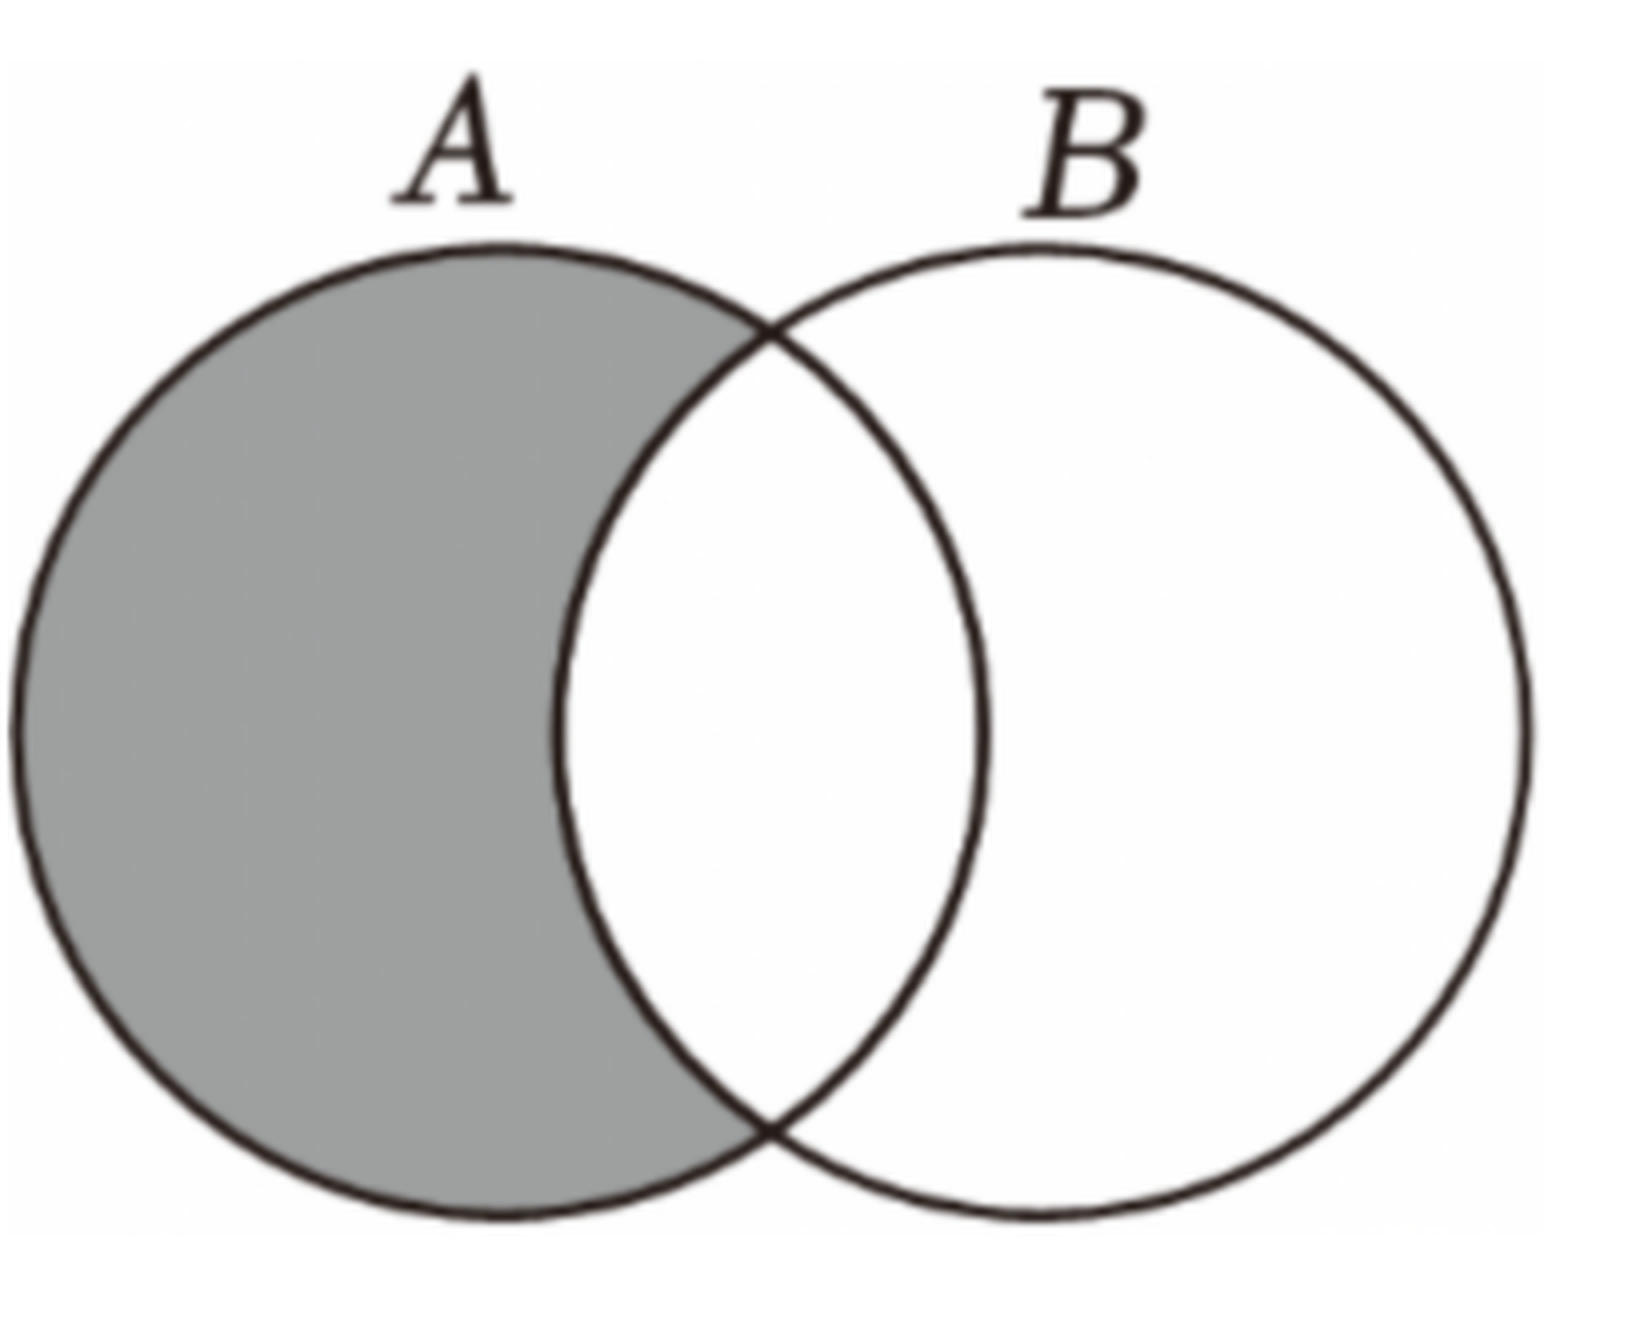
\includegraphics[width=0.30\textwidth]{figures/venn_A_minus_B_h38.png}
\end{center}

\ans{$\{1\}$}

\item 集合 $\{2,3,4,\cdots,2024,2025\}$ 的真子集的个数为 \blankline[4.4em].

\ans{$2^{2024}-1$}

\ifanswer
\solbegin
\step{集合 $\{2,3,4,\cdots,2024,2025\}$ 的真子集的个数为 $2^{2024}-1$.}
\solend

\fi

\item 已知集合 $A$ 中的元素都是正整数，其中最小的是 $1$，最大值是 $100$，除 $1$ 以外，每一个元
素都等于 $A$ 中的两个数（可以相同）的和，则集合 $A$ 中至少含有 \blankline[4.4em] 个元素.

\ans{$9$}

\ifanswer
\solbegin
\step{设 $A$ 中的数从小到大排列为 $1,a_1,a_2,\cdots,a_k,100$，}
\step{则 $a_1=1+1=2$；$3\leqslant a_2\leqslant 4$；$4\leqslant a_3\leqslant 8$；$5\leqslant a_4\leqslant 16$；$6\leqslant a_5\leqslant 32$；$7\leqslant a_6\leqslant 64$；}
\step{于是 $A$ 至少有八个数；}
\step{假设 $A$ 恰好有八个元素，由于 $a_5+a_6\leqslant 96<100$；}
\step{故必须有 $100=a_6+a_6$，$a_6=50$，}
\step{又 $a_4+a_5\leqslant 48$，同理 $a_5=25$，}
\step{但此时 $a_3+a_4\leqslant 24$，$a_5=2a_4$，$a_4=12.5$ 矛盾，}
\step{故 $A$ 不可能恰好有八个元素，因此 $A$ 至少有九个元素.}
\step{其九个数可以为 $1$，$2$，$3$，$6$，$12$，$13$，$25$，$50$，$100$.}
\solend

\fi

\item 已知集合 $\{x_1,x_2,x_3,x_4,x_5,x_6\}=\{1,2,3,4,5,6\}$，将 $x_i$ 与 $x_j$（其中 $i\in\{1,2,3\}$，
$j\in\{4,5,6\}$）的乘积 $x_ix_j$ 放入如图的 $3\times3$ 方格中，则方格中全部数之和的最大值为 \blankline[4.4em].

% 原卷的 $3\times3$ 方格是表格式内容（三行三列的公式），本稿按 高一03 的成例用 tabular 排出。
\begin{center}
\begin{tabular}{|c|c|c|}
\hline
$x_1x_4$ & $x_1x_5$ & $x_1x_6$ \\
\hline
$x_2x_4$ & $x_2x_5$ & $x_2x_6$ \\
\hline
$x_3x_4$ & $x_3x_5$ & $x_3x_6$ \\
\hline
\end{tabular}
\end{center}

\ans{$110$}

\ifanswer
\solbegin
\step{由表格数据得所有数之和为}
\step{$S=x_1x_4+x_1x_5+x_1x_6+x_2x_4+x_2x_5+x_2x_6+x_3x_4+x_3x_5+x_3x_6$，}
\step{所以 $S=(x_1+x_2+x_3)(x_4+x_5+x_6)$，}
\step{因为集合 $\{x_1,x_2,x_3,x_4,x_5,x_6\}=\{1,2,3,4,5,6\}$，}
\step{所以 $x_1+x_2+x_3+x_4+x_5+x_6=1+2+3+4+5+6=21$，}
\step{设 $t=x_1+x_2+x_3$，则 $6\leqslant t\leqslant 15$，$t\in\N^*$，}
\step{$S=t(21-t)=-\left(t-\dfrac{21}{2}\right)^2+\dfrac{441}{4}$，}
\step{当 $t=10$ 或 $t=11$ 时，$S=t(21-t)$ 取最大值，最大值为 $110$，}
\step{此时 $\{x_1,x_2,x_3\}=\{1,4,5\}$，$t=10$，所以可取最大值 $110$.}
\solend

\fi

\item 若 $[x]$ 表示不大于 $x$ 的最大整数，方程 $x^2-8[x]+7=0$ 的解集为 \blankline[4.4em].

\ans{$\{1,\sqrt{33},\sqrt{41},7\}$}

\ifanswer
\solbegin
\step{由题意，$x\geqslant[x]=\dfrac{x^2+7}{8}>0$，得 $x^2-8x+7\leqslant 0$，解得 $1\leqslant x\leqslant 7$，}
\step{$[x]=1$，$x^2=1$，$x=1$；}
\step{$[x]=2$，$x^2=9$，$x=3$ 与 $[x]=2$ 矛盾；}
\step{$[x]=3$，$x^2=17$，$x=\sqrt{17}$，$[x]=4$ 与 $[x]=3$ 矛盾；}
\step{$[x]=4$，$x^2=25$，$x=5$ 与 $[x]=4$ 矛盾；}
\step{$[x]=5$，$x^2=33$，$x=\sqrt{33}$，$[x]=5$；}
\step{$[x]=6$，$x^2=41$，$x=\sqrt{41}$，$[x]=6$；}
\step{$[x]=7$，$x^2=49$，$x=7$；}
\step{综上，方程 $x^2-8[x]+7=0$ 的解集为 $\{1,\sqrt{33},\sqrt{41},7\}$.}
\solend

\fi

\end{enumerate}

\bigsec{二、选择题}

\begin{enumerate}
\setcounter{enumi}{10}

\item 已知集合 $A=\{a,a^2\}$，$B=\{1,3\}$，若 $1\in A$，则 $A\cup B$ 中所有元素之和为\mbox{（\quad）}

\keepwithprev
A. $2$\qquad B. $3$\qquad C. $4$\qquad D. $5$

\ans{$B$}

\ifanswer
\solbegin
\step{因为 $1\in A$，集合 $A=\{a,a^2\}$，所以 $a=1$ 或 $a^2=1$，}
\step{若 $a=1$，则 $a=a^2$，与元素的互异性矛盾；}
\step{若 $a^2=1$，则 $a=1$（舍）或 $a=-1$，故 $A=\{-1,1\}$，$B=\{1,3\}$，}
\step{故 $A\cup B=\{-1,1,3\}$，所以 $A\cup B$ 中所有元素之和为 $-1+1+3=3$. 故选 $B$.}
\solend

\fi

\item 对于实数 $a$、$b$、$c$，下列命题正确的是\mbox{（\quad）}

\keepwithprev
A. 若 $a>b$，则 $ac^2>bc^2$\qquad B. 若 $a>b$，则 $a^2>b^2$

C. 若 $a>b$，则 $a|a|>b|b|$\qquad D. 若 $a>b>c>0$，则 $\dfrac{b}{a-b}<\dfrac{c}{a-c}$

\ans{$C$}

\ifanswer
\solbegin
\step{对于 $A$，若 $a>b$，$c=0$，则 $ac^2=bc^2$，故 $A$ 错误；}
\step{对于 $B$，若 $a>b$，取 $a=-1$，$b=-2$，则 $a^2<b^2$，故 $B$ 错误；}
\step{对于 $C$，若 $a>b>0$ 时，$a|a|-b|b|=a^2-b^2>0$，}
\step{当 $a>0>b$ 时，$a|a|-b|b|=a^2+b^2>0$，}
\step{当 $0>a>b$ 时，$a|a|-b|b|=b^2-a^2=(b-a)(b+a)>0$，}
\step{综上，若 $a>b$，则 $a|a|>b|b|$，故 $C$ 正确；}
\step{对于 $D$，若 $a>b>c>0$，$\dfrac{b}{a-b}-\dfrac{c}{a-c}=\dfrac{ab-bc-ac+bc}{(a-b)(a-c)}=\dfrac{a(b-c)}{(a-b)(a-c)}>0$，}
\step{故 $D$ 错误.}
\step{故选 $C$.}
\solend

\fi

\item 对于正整数集合 $A=\{a_1,a_2,\cdots,a_n\}(n\in\N^*,\ n\geqslant 3)$，如果去掉其中任意一个元素
$a_i(i=1,2,\cdots,n)$ 之后，剩余的所有元素组成的集合都能分为两个交集为空集的集合，且这
两个集合的所有元素之和相等，就称集合 $A$ 为平衡集. 记 $M=a_1+a_2+\cdots+a_n$. 若集合 $A$
是平衡集，并且存在 $a_i$ 为奇数，则集合 $A$ 中元素个数 $n$ 的奇偶性\mbox{（\quad）}

\keepwithprev
A. 与 $M$ 相关，既可以是奇数，又可以是偶数

B. 与 $M$ 无关，既可以是奇数，又可以是偶数

C. 与 $M$ 无关，必为偶数

D. 与 $M$ 无关，必为奇数

\ans{$D$}

\ifanswer
\solbegin
\step{正整数集合 $A=\{a_1,a_2,\cdots,a_n\}(n\in\N^*,\ n\geqslant 3)$，}
\step{因为集合 $A$ 是平衡集，设去掉元素 $a_i(i=1,2,\cdots,n)$，}
\step{由题意得 $A=A_1\cup A_2\cup\{a_i\}$，其中 $A_1\cap A_2=\varnothing$，}
\step{设集合 $A_1$ 和 $A_2$ 中的元素之和均为 $m$，所以 $M=2m+a_i$，其中 $i=1,2,\cdots,n$，}
\step{所以 $M-a_i=2m$，所以 $M-a_i$ 为偶数，其中 $i=1,2,\cdots,n$，}
\step{所以 $a_i(i=1,2,\cdots,n)$ 的奇偶性相同；}
\step{因为存在 $a_i$ 为奇数，所以 $a_i(i=1,2,\cdots,n)$ 均为奇数，}
\step{由 $M-a_i=2m$ 得 $M$ 也为奇数，且 $M=a_1+a_2+\cdots+a_n$，}
\step{所以 $n$ 也为奇数，所以 $n$ 必为奇数. 故选 $D$.}
\solend

\fi

\item 对于集合 $M=\{a\mid a=x^2-y^2,\ x\in\Z,\ y\in\Z\}$，给出如下三个结论：其中正确结论的个数
是\mbox{（\quad）}

\keepwithprev
①如果 $P=\{b\mid b=2n+1,\ n\in\Z\}$，那么 $P\sub M$；

②如果 $c=4n+2$，$n\in\Z$，那么 $c\notin M$；

③如果 $a_1\in M$，$a_2\in M$，那么 $a_1a_2\in M$.

\keepwithprev
A. $1$\qquad B. $2$\qquad C. $3$\qquad D. $0$

\ans{$C$}

\ifanswer
\solbegin
\step{对于①，$b=2n+1$，$n\in\Z$，则恒有 $2n+1=(n+1)^2-n^2$，}
\step{所以 $2n+1\in M$，即 $P=\{b\mid b=2n+1,n\in\Z\}$，则 $P\sub M$，①正确；}
\step{对于②，$c=4n+2$，$n\in\Z$，}
\step{若 $4n+2\in M$，则存在 $x$、$y\in\Z$ 使得 $x^2-y^2=4n+2$，}
\step{所以 $4n+2=(x+y)(x-y)$，又 $x+y$ 和 $x-y$ 同奇或同偶，}
\step{若 $x+y$ 和 $x-y$ 都是奇数，则 $(x+y)(x-y)$ 为奇数，而 $4n+2$ 是偶数；}
\step{若 $x+y$ 和 $x-y$ 都是偶数，则 $(x+y)(x-y)$ 能被 $4$ 整除，而 $4n+2$ 不能被 $4$ 整除，}
\step{所以 $4n+2\notin M$，即 $c\notin M$，②正确；}
\step{对于③，$a_1\in M$，$a_2\in M$，可设 $a_1=x_1^2-y_1^2$，$a_2=x_2^2-y_2^2$，$x_i$、$y_i\in\Z$；}
\step{则 $a_1a_2=(x_1^2-y_1^2)(x_2^2-y_2^2)=(x_1x_2)^2+(y_1y_2)^2-(x_1y_2)^2-(x_2y_1)^2$}
\step{$=(x_1x_2+y_1y_2)^2-(x_1y_2+x_2y_1)^2\in M$，那么 $a_1a_2\in M$，③正确.}
\step{综上，正确的命题是①②③. 故选 $C$.}
\solend

\fi

\end{enumerate}

\bigsec{三、解答题}

\begin{enumerate}
\setcounter{enumi}{14}

\item 已知 $A=\{x\mid a\leqslant x\leqslant -a+3\}$，$B=\{x\mid x<-1\text{ 或 }x>5\}$.

\begin{enumerate}[label=(\arabic*)]

\item 若 $A\cap B=\varnothing$，求 $a$ 的取值范围；

\item 若 $A\cup B=\R$，求 $a$ 的取值范围.

\end{enumerate}

\ans{（1）$[-1,+\infty)$；（2）$(-\infty,-2]$}

\ifanswer
\solbegin
\stepm{(1)}{①当 $A=\varnothing$ 时，$A\cap B=\varnothing$，需满足 $a>-a+3$，解得 $a>\dfrac32$，}
\step{故 $a$ 的取值范围为 $\left(\dfrac32,+\infty\right)$.}
\step{②当 $A\neq\varnothing$ 时，要使 $A\cap B=\varnothing$，需满足
$\begin{cases}a\leqslant\dfrac32\\[4pt] -a+3\leqslant 5\\[4pt] a\geqslant -1\end{cases}$，解得 $-1\leqslant a\leqslant\dfrac32$.}
\step{综上所述，$a$ 的取值范围是 $[-1,+\infty)$.}
\stepm{(2)}{因为 $A\cup B=\R$，$A=\{x\mid a\leqslant x\leqslant -a+3\}$，$B=\{x\mid x<-1\text{ 或 }x>5\}$，}
\step{所以 $\begin{cases}-a+3\geqslant 5\\[4pt] a\leqslant -1\end{cases}$，解得 $a\leqslant -2$，故所求 $a$ 的取值范围为 $(-\infty,-2]$.}
\solend

\fi

\ansspace[6]

\item 已知集合 $A=\{x\mid mx^2+x-2=0\}$，$B=\{x\mid 2x^2-5x-12=0\}$.

\begin{enumerate}[label=(\arabic*)]

\item 若 $A$ 中有且仅有 $1$ 个元素，求实数 $m$ 的值；

\item 已知集合 $C=A\cup B$，若 $C$ 的真子集有且仅有 $3$ 个，求实数 $m$ 的取值范围.

\end{enumerate}

\ans{（1）$m=0$ 或 $m=-\dfrac18$；（2）$\left\{m\mid m\leqslant -\dfrac18\right\}$}

\ifanswer
\solbegin
\stepm{(1)}{若 $m=0$，方程化为 $x-2=0$，此时方程有且仅有一个根 $x=2$；}
\step{若 $m\neq 0$，则 $\Delta=1^2-4\times m\times(-2)=0$，即 $m=-\dfrac18$ 时，}
\step{方程有两个相等的实根，此时集合 $A$ 中有且仅有一个元素，}
\step{所以实数 $m$ 的值为 $m=0$ 或 $m=-\dfrac18$；}
\stepm{(2)}{$B=\{x\mid 2x^2-5x-12=0\}=\left\{-\dfrac32,4\right\}$，}
\step{因为 $C=A\cup B$，若 $C$ 的真子集有且仅有 $3$ 个，则 $C$ 中有两个元素，}
\step{所以 $A\sub B$，由（1）得 $m=0$ 时，$A=\{2\}$，不符合 $A\sub B$，}
\step{当 $m\neq 0$ 时，若 $\Delta=1^2-4\times m\times(-2)<0$，解得 $m<-\dfrac18$，}
\step{此时 $A=\varnothing$，符合 $A\sub B$，}
\step{若 $\Delta=1^2-4\times m\times(-2)=0$，解得 $m=-\dfrac18$，}
\step{此时方程 $mx^2+x-2=0$ 的根为 $x=4$，集合 $A=\{4\}$，符合 $A\sub B$，}
\step{若 $\Delta=1^2-4\times m\times(-2)>0$，由 $A\sub B$，得 $A=\left\{-\dfrac32,4\right\}$，}
\step{此时有 $-\dfrac32+4=-\dfrac1m$ 且 $-\dfrac32\times 4=-\dfrac2m$，无解，}
\step{综上所述，实数 $m$ 的取值范围为 $\left\{m\mid m\leqslant -\dfrac18\right\}$.}
\solend

\fi

\ansspace[6]

\item 设 $A$ 是非空实数集，且 $0\notin A$. 若对于任意的 $x$、$y\in A$，都有 $xy\in A$，则称集合 $A$ 具
有性质 $P_1$；若对于任意的 $x$、$y\in A$，都有 $\dfrac xy\in A$，则称集合 $A$ 具有性质 $P_2$.

\begin{enumerate}[label=(\arabic*)]

\item 写出一个恰含有两个元素且具有性质 $P_1$ 的集合 $A$，并说明理由；

\item 证明：“非空实数集 $A$ 具有性质 $P_1$”是“非空实数集 $A$ 具有性质 $P_2$”的必要非充分条
件.

\end{enumerate}

\ans{（1）$A=\{-1,1\}$，理由见解析；（2）见解析}

\ifanswer
\solbegin
% 注：原卷本题 (1) 的解析里“证明”一词重复出现两次（一次接在分号后、一次另起一行），
%     本稿照原卷重复录入，未去重。
\stepm{(1)}{$A=\{-1,1\}$，证明：恰含有两个元素且具有性质 $P_1$ 的集合 $A=\{-1,1\}$；}
\step{证明：$1\times 1=1\in A$，$1\times(-1)=-1\in A$，$-1\times 1=-1\in A$，$-1\times(-1)=1\in A$；}
\stepm{(2)}{若集合 $A$ 具有性质 $P_2$，不妨设 $a\in A$，}
\step{由非空数集 $A$ 具有性质 $P_2$，有 $\dfrac aa=1\in A$.}
\step{①$A=\{1\}$，易得此时集合 $A$ 具有性质 $P_1$.}
\step{②数集 $A$ 只含有两个元素，不妨设 $A=\{1,a_1\}$，}
\step{由 $\dfrac{1}{a_1}=a_1$，且 $a_1\neq 1$，解得 $a_1=-1$，此时集合 $A$ 具有性质 $P_1$.}
\step{③实数集 $A$ 含有两个以上的元素，不妨设不为 $1$ 的元素 $a_1$、$a_2\in A$，}
\step{则有 $\dfrac{1}{a_1}\in A$，由于集合 $A$ 具有性质 $P_2$，}
\step{所以有 $a_2\div\dfrac{1}{a_1}=a_1a_2\in A$，这说明集合 $A$ 具有性质 $P_1$.}
\step{综上，若非空实数集 $A$ 具有性质 $P_2$，则集合 $A$ 具有性质 $P_1$，}
\step{所以“非空实数集 $A$ 具有性质 $P_1$”是“非空实数集 $A$ 具有性质 $P_2$”的}
\step{必要条件.}
\step{取正偶数集 $A=\{x\mid x=2n,\ n\in\N^*\}$，}
\step{对任意的 $2m$、$2n\in A$，$m$、$n\in\N^*$，}
\step{有 $2m\times 2n=4mn\in A$，故 $A$ 具有性质 $P_1$，}
\step{取 $x=2$，$y=4$，则 $\dfrac xy=\dfrac12\notin A$，故 $A$ 不具有性质 $P_2$，}
\step{所以“非空实数集 $A$ 具有性质 $P_1$”不是“非空实数集 $A$ 具有性质 $P_2$”的}
\step{充分条件.}
\step{综上，“非空实数集 $A$ 具有性质 $P_1$”是“非空实数集 $A$ 具有性质 $P_2$”的}
\step{必要非充分条件.}
\solend

\fi

\ansspace[8]

\item 已知命题 $p$：关于 $x$ 的方程 $x^2+mx+1=0$ 有两个不同的正根；命题 $q$：关于 $x$ 的方程
$4x^2+4(m-2)x=-1$ 有实根.

\begin{enumerate}[label=(\arabic*)]

\item 若命题 $q$ 为假命题，求整数 $m$ 的解集；

\item 若命题 $p$ 为真命题，且关于 $x$ 的方程 $x^2+mx+1=0$ 的两个实数根 $x_1$、$x_2$ 满足
$3x_1+2x_2=5$，求实数 $m$ 的取值集合；

\item 若命题 $p$ 和命题 $q$ 有且仅有一个成立，求实数 $m$ 的取值范围.

\end{enumerate}

\ans{（1）$\{2\}$；（2）$\left\{-\dfrac{13}{6}\right\}$；（3）$[-2,1]\cup[3,+\infty)$}

\ifanswer
\solbegin
\stepm{(1)}{命题 $q$：关于 $x$ 的方程 $4x^2+4(m-2)x=-1$ 有实根为假命题，}
\step{即 $4x^2+4(m-2)x+1=0$ 无实根，}
\step{则 $\Delta=16(m-2)^2-16<0$，则 $1<m<3$，则整数 $m$ 的解集为 $\{2\}$；}
\stepm{(2)}{若命题 $p$ 为真命题，且关于 $x$ 的方程 $x^2+mx+1=0$ 的两个实数根 $x_1$、$x_2$，}
\step{满足 $3x_1+2x_2=5$，则方程 $x^2+mx+1=0$ 有两个不同的正根，}
\step{则 $\begin{cases}\Delta=m^2-4>0\\[4pt] x_1+x_2=-m>0\end{cases}$，则 $m<-2$，}
\step{又 $\begin{cases}x_1+x_2=-m\\[4pt] x_1x_2=1\\[4pt] 3x_1+2x_2=5\end{cases}$，
则 $\begin{cases}x_1=5+2m\\[4pt] x_2=-3m-5\end{cases}$，则 $(5+2m)(-3m-5)=1$，}
\step{得 $m=-2$ 或 $m=-\dfrac{13}{6}$，又因为 $m<-2$，所以 $m=-\dfrac{13}{6}$，}
\step{所以实数 $m$ 的取值集合为 $\left\{-\dfrac{13}{6}\right\}$；}
\stepm{(3)}{由（2）得当 $p$ 为真时，则有 $m<-2$，}
\step{当 $q$ 为真时，$\Delta=16(m-2)^2-16\geqslant 0$，解得 $m\leqslant 1$ 或 $m\geqslant 3$，}
\step{又因为命题 $p$ 和命题 $q$ 只有一个为真，所以
$\begin{cases}m<-2\\[4pt] 1<m<3\end{cases}$ 或 $\begin{cases}m\geqslant -2\\[4pt] m\leqslant 1\text{ 或 }m\geqslant 3\end{cases}$，}
\step{解得 $-2\leqslant m\leqslant 1$ 或 $m\geqslant 3$，所以实数 $m$ 的取值范围为 $[-2,1]\cup[3,+\infty)$.}
\solend

\fi

\ansspace[8]

% 注：原卷此处作“设 $n\in\N^*$，集合含有 $3n$ 个元素”，**漏了符号 $U$**（应作“集合 $U$
%     含有 $3n$ 个元素”）——$U$ 直到本句末尾“则称 $U$ 为三分集合”才出现、此前无定义。
%     本稿照录未补，见文件头“原卷笔误/存疑”⑦。
\item 设 $n\in\N^*$，集合含有 $3n$ 个元素，若存在三个 $n$ 元集合 $A$、$B$、$C$ 满足如下两个条件，
则称 $U$ 为三分集合.

①$U=A\cup B\cup C$；

②$A$、$B$、$C$ 元素可分别排列为有序数组 $(a_1,a_2,\cdots,a_n)$，$(b_1,b_2,\cdots,b_n)$ 及
$(c_1,c_2,\cdots,c_n)$，使得对 $\forall i=1,2,\cdots,n$，均有 $a_i+b_i=c_i$.

特别地，当 $U=\{1,2,3,4,\cdots,3n-2,3n-1,3n\}$ 为三分集合时，称 $n$ 为完美三分数.

如：因为 $U=\{1,2,3\}$ 为三分集合，所以 $n=1$ 为最小完美三分数.

\begin{enumerate}[label=(\arabic*)]

\item 请判断下列两个集合是否为三分集合（直接写出结论）：

$U_1=\{1,2,3,4,5,6\}$，$U_2=\{1,3,5,7,8,9,10,11,12\}$；

\item 求出大于 $1$ 的最小完美三分数；

\item 请判断是否存在无穷多个完美三分数？若存在，请说明理由；若不存在，则求出最大的
完美三分数.

\end{enumerate}

\ans{（1）$U_1$ 不是三分集合，$U_2$ 是三分集合；（2）$4$；（3）存在，理由见解析}

\ifanswer
\solbegin
\stepm{(1)}{(i)$U_1=\{1,2,3,4,5,6\}$ 不是三分集合，下面用反证法证明：}
\step{证明：假设 $U=\{1,2,3,4,5,6\}$ 是三分集合，}
\step{设 $A=\{a_1,a_2\}$，$B=\{b_1,b_2\}$，$C=\{c_1,c_2\}$，不妨设 $c_1<c_2$，}
\step{因为 $a_1+b_1=c_1$，$a_2+b_2=c_2$，}
\step{所以 $a_1+b_1+a_2+b_2+c_1+c_2=2(c_1+c_2)=1+2+3+4+5+6=21$，}
% 注：原卷此步印“所以 $c_1+c_2=2$”，与上一行的 $2(c_1+c_2)=21$ **不自洽**
%     （应作 $\dfrac{21}2$）；同题 $n=3$ 处的同型推理原卷写的是 $\dfrac{45}2$，故此处是原卷笔误。
%     本稿照录未改，见文件头“原卷笔误/存疑”⑧。
\step{所以 $c_1+c_2=2$，这与 $c_1,c_2\in\N^*$ 矛盾，故假设错误，}
\step{故 $U_1=\{1,2,3,4,5,6\}$ 不是三分集合；}
\step{(ii)$U_2=\{1,3,5,7,8,9,10,11,12\}$ 是三分集合，理由如下：}
\step{令 $A=\{1,3,5\}$，$B=\{9,8,7\}$，$C=\{10,11,12\}$，}
\step{则 $A\cup B\cup C=U=\{1,3,5,7,8,9,10,11,12\}$，满足条件①；}
\step{又 $1+9=10$；$3+8=11$；$5+7=12$，所以满足条件②，}
\step{所以 $U_2=\{1,3,5,7,8,9,10,11,12\}$ 是三分集合；}
\stepm{(2)}{由（1）得，当 $n=2$ 时，$U=\{1,2,3,4,5,6\}$ 不是三分集合；}
\step{当 $n=3$ 时，$U=\{1,2,3,4,5,6,7,8,9\}$，}
\step{假设 $U=\{1,2,3,4,5,6,7,8,9\}$ 是三分集合，}
\step{同理由 $a_1+b_1+a_2+b_2+a_3+b_3+c_1+c_2+c_3$}
\step{$=2(c_1+c_2+c_3)=1+2+\cdots+9=45$，$c_1+c_2+c_3=\dfrac{45}{2}$，}
\step{可推出与 $c_1$、$c_2$、$c_3\in\N^*$ 矛盾，故假设也错误，}
\step{所以 $U=\{1,2,3,4,5,6,7,8,9\}$ 不是三分集合；}
\step{当 $n=4$ 时，$U=\{1,2,3,\cdots,12\}$，}
\step{存在三个 $4$ 元集合 $A=\{1,2,4,3\}$，$B=\{5,8,7,9\}$，$C=\{6,10,11,12\}$，}
\step{满足 $U=\{1,2,3,\cdots,12\}$ 为三分集合的两个条件，}
\step{故大于 $1$ 的最小完美三分数为 $4$；}
\stepm{(3)}{存在无穷多个完美三分数，理由如下：}
\step{由题意得，$n=1$ 为最小完美三分数，}
\step{当 $n=5$ 时，$U=\{1,2,3,\cdots,15\}$，}
\step{存在三个 $5$ 元集合 $A=\{1,3,5,7,2\}$，$B=\{11,10,9,8,4\}$，$C=\{12,13,14,15,6\}$，}
\step{满足三分集合的条件，故 $5$ 为完美三分数；}
\step{当 $n=21$ 时，$U=\{1,2,3,\cdots,63\}$，}
\step{存在如下三个 $21$ 元的集合满足三分集合的条件：}
\step{$A=\{1,3,5,7,\cdots,29,31,2,6,10,14,4\}$，}
\step{$B=\{47,46,45,44,\cdots,33,32,22,20,18,16,8\}$，}
\step{$C=\{48,49,50,51,\cdots,62,63,24,26,28,30,12\}$，}
\step{故 $21$ 为完美三分数.}
\step{首先证明：若 $n=k$，$k\in\N^*$ 为三分完美数，}
\step{则 $n=4k+1$，$k\in\N^*$ 也为三分完美数，}
% 注：下一行原卷印作“$U_{k+1}=U_{k+1}=\{2,3,\cdots,12k+3\}$”——等号两边记号相同，
%     依上下文疑当作 $U'_{k+1}=U_{4k+1}$，且此处集合自 2 起（前文 $U_{4k+1}$ 自 1 起）；
%     本稿照录原卷，未代为改写。
\step{证明：记 $U_k=\{1,2,3,\cdots,3k\}$，$U_{4k+1}=\{1,2,3,\cdots,12k+3\}$，}
\step{若 $n=k$，$k\in\N^*$ 为三分完美数，则 $U_k$ 为三分集合，}
\step{即存在三个 $k$ 元集合 $A$、$B$、$C$ 满足如下两个条件，}
\step{①$U_k=A\cup B\cup C$；}
\step{②$A$、$B$、$C$ 元素可分别排列为有序数组 $(a_1,a_2,\cdots,a_k)$，}
\step{$(b_1,b_2,\cdots,b_k)$ 及 $(c_1,c_2,\cdots,c_k)$，}
\step{使得对 $\forall i=1,2,3,\cdots,k$，均有 $a_i+b_i=c_i$，}
\step{则可得到对 $\forall i=1,2,3,\cdots,k$，$2a_i+2b_i=2c_i$，}
\step{故集合 $\{2,4,6,\cdots,6k\}$ 也满足三分集合的两个条件，其也为三分集合，}
\step{下面记集合 $\{2,4,6,\cdots,6k\}=2U_k$，}
\step{对 $n=4k+1$，集合 $U_{k+1}=U_{k+1}=\{2,3,\cdots,12k+3\}=(2U_k)\cup\complement_{U_{4k+1}}(2U_k)$，}
\step{构造集合 $A'=\{1,3,5,7,\cdots,6k+1\}$，共有 $3k+1$ 个奇数；}
% 注：下一行原卷印作“$B'=\{6k+3k+2,6k+3k+1,6k+3k,6k+3k-1,\cdots,6k+2\}$”，
%     按与后文 $C'$ 相接，前四项当写作 $9k+2$、$9k+1$、$9k$、$9k-1$；本稿照录原卷。
\step{集合 $B'=\{6k+3k+2,6k+3k+1,6k+3k,6k+3k-1,\cdots,6k+2\}$，}
\step{共有 $3k+1$ 个逐个减小的连续正整数；}
\step{集合 $C'=\{9k+3,9k+4,9k+5,9k+6,\cdots,12k+3\}$，}
\step{共有 $3k+1$ 个逐个增大的连续正整数；}
\step{得这三个 $3k+1$ 元集合 $A'$、$B'$、$C'$ 满足如下两个条件，}
\step{①集合 $A'\cup B'\cup C'=\complement_{U_{4k+1}}(2U_k)$；}
\step{②$A'$、$B'$、$C'$ 元素可分别排列为有序数组 $(a_1,a_2,\cdots,a_{3k+1})$，}
\step{$(b_1,b_2,\cdots,b_{3k+1})$ 及 $(c_1,c_2,\cdots,c_{3k+1})$，}
\step{使得对 $\forall i=1,2,3,\cdots,3k+1$，均有 $a_i+b_i=c_i$；}
\step{故 $\complement_{U_{4k+1}}(2U_k)$ 为三分集合，而已知 $U_k$ 为三分集合，}
\step{将其对应与 $A'$、$B'$、$C'$ 合并，}
% 注：原卷此处印“令 $A''=A\cup A'$”（$B''$、$C''$ 同）。按同段上文“记集合
%     $\{2,4,6,\cdots,6k\}=2U_k$”，此处疑当作 $A''=2A\cup A'$——否则
%     $A''\cup B''\cup C''=U_k\cup\complement_{U_{4k+1}}(2U_k)\neq U_{4k+1}$，与本段结论冲突。
%     本稿照录未改，见文件头“原卷笔误/存疑”⑨。
\step{令 $A''=A\cup A'$，$B''=B\cup B'$，$C''=C\cup C'$，}
\step{则这三个 $4k+1$ 元集合 $A''$、$B''$、$C''$，}
\step{满足 $A''\cup B''\cup C''=U_{4k+1}$，且满足条件②，}
\step{故 $U_{4k+1}=\{1,2,3,\cdots,12k+3\}$ 为三分集合，}
\step{因此可得，若 $n=k$ 为三分完美数，则 $n=4k+1$ 也为三分完美数，}
\step{由 $1$，$5$，$21$ 为完美三分数，结合所证结论得，存在无穷多个完美三分数.}
\solend

\fi

\ansspace*[12]

\end{enumerate}

\end{document}
"
% 紧凑版：xelatex "\def\iscompact{1}% 高一38_大同中学_周末作业3.tex
%   —— 高一上数学“2026-2027 年大同中学高一上周末作业 3”（试卷版/答案版）
% 试卷版：xelatex 高一38_大同中学_周末作业3.tex
% 答案版：xelatex "\def\isanswer{1}\input{高一38_大同中学_周末作业3.tex}"
% 紧凑版：xelatex "\def\iscompact{1}\input{高一38_大同中学_周末作业3.tex}"
%
% 原始材料是微信公众号图文（公众号“魔都数学加油站”连载“27学年高一 38”，署名“破晓”，
% 2026-09-26 21:29 发布，原文标题“27学年高一38——2026-2027年上海市大同中学高一上周末作业3”，
% 原文链接 https://mp.weixin.qq.com/s/O_O60vCIiGi2xponAo4irw ），正文为 12 张 PNG 页。
% **同一篇里各页分辨率不一致**（2560×3620 与 4762×6735 两档混排：第 1、10、11、12 页为
% 2560×3620，第 2—9 页为 4762×6735）。原文本身就是一份**讲评版**——有的题下方只印
% 【答案】行，有的只印【解析】。试题文字、答案与解析均照原卷录入，未改内容。卷面的粉色
% 斜水印“魔都数学加油站”属水印，未录入。
%
% 本卷共 **17 题**：填空题 8 题（第 3—10 题）、选择题 4 题（第 11—14 题）、解答题 5 题
% （第 15—19 题）；插图 1 张（第 6 题 Venn 图）。三版页数：试卷版 4 页 / 答案版 11 页 /
% 紧凑版 3 页，`Overfull`／`Underfull`／`Missing character` 告警均为 0。
%
% 卷首标题：原卷印作“2026-2027 年大同中学高一上周末作业 3”（公众号原文标题里的“上海市”
% 三字卷面标题行没有，本稿照卷面），年份区间按全稿惯例排 en dash，前缀照原卷保留“年”。
%
% 与原卷的排版差异（均已在 README“说明”中交代）：
%   ① 原文自**第 3 题**起（第 1、2 题未在该文中发布），故本稿题号亦自 3 起，填空题以
%      \setcounter{enumi}{2} 起编；选择、解答两节各按上一节末号另设 \setcounter
%      （选择题 \setcounter{enumi}{10}、解答题 \setcounter{enumi}{14}）；
%   ② 原卷本就印有“一、填空题”“二、选择题”“三、解答题”三节标题，本稿照原卷分节，
%      只把标题改排成全稿统一的“大节标题”样式；
%   ③ 原卷是“讲评版”：第 3、6 题只印【答案】行，第 4、5、7、8、9、10 题与第 11—19 题印
%      【解析】；本稿统一改为试卷版隐去、答案版以 \ans{}／\ifanswer 块给出，两版彻底分离。
%      其中第 4、5、7、8、9、10 题与第 11—14 题的答案，原卷写在【解析】末句，本稿另提为
%      \ans{}；第 15—19 题原卷只有【解析】、无独立答案行，本稿亦补了摘要式 \ans{}。
%      **故本卷 17 题每题都有 \ans**——比“只印【解析】的填空、解答题不另提 \ans”的
%      高一31／高一34 更彻底，与 高一21 第 11 题（填空，答案在【解析】末句，本稿另提）同类；
%      （本仓对“另提 \ans{}”的做法各卷不一，见 README 对应专记的核对面。）
%   ④ 数集记号原卷两套并用：第 3、5 题的实数集作粗体 $\mathbf{R}$，第 8、14、17、18 题等的
%      整数集、自然数集作斜体 $Z$、$N$，本稿按全稿惯例统一写作 $\R$、$\Z$、$\N$；
%   ⑤ 原卷填空的横线宽度不一（约 1.8—3.6 字宽），本稿按全稿惯例统一排 \blankline[4.4em]；
%   ⑥ 中文括注原卷用半角“(  )”，本稿按全稿惯例排全角；选择题的作答括注统一排
%      \mbox{（\quad）}（第 14 题的作答括注原卷印在 ①②③ 三个命题**之前**，本稿照原卷次序）；
%      数学式内部的括注（如第 4 题的 $p\%(0<p<100)$、第 13 题的 $a_i(i=1,2,\cdots,n)$）照原样
%      留在行内公式里，未改全角；
%   ⑦ 原卷并列的字母（“x,y”“a,b,c”）不加标点或作半角逗号，本稿按全稿惯例改排顿号；
%   ⑧ 第 6 题的 Venn 图取原卷截图、4× LANCZOS 放大（figures/venn_A_minus_B_h38.png，
%      见该处 \includegraphics 前的注释）；第 9 题的 $3\times3$ 方格属**表格式**内容，
%      本稿按 高一03 的成例用 tabular 排出，未截图；
%   ⑨ 原卷未印副标题，本稿按**本卷实际内容**补出副标题“集合与常用逻辑用语”（依据见下条）；
%   ⑩ 原卷【解析】**一个印刷行照录为一条 `\step`**（原卷的折行也照录为独立一条，如第 17 题
%      末三处“…的”／“必要条件.”这类跨行句、第 9 题“由表格数据得所有数之和为”／
%      “$S=\cdots$，”），使答案版的排布与原卷讲评版逐行对应；全卷 15 处【解析】合计
%      **191 条 `\step` ＝ 原卷 191 行**（逐处：5、5、1、9、9、9、4、9、9、12、6、14、21、13、65）。
%
% 副标题（\examtitlest 第二个参数）：本卷卷面未印副标题，由本稿补出，取值按 2026-09-26 起的
%   新口径“只用本卷实际内容的模块名”定为“集合与常用逻辑用语”。依据：全卷 17 题
%   （第 3—19 题）中，第 3、5、6、7、8、9、10、11、13、14、15、16、17、18、19 题共 15 题
%   是集合的运算与关系、子集计数、集合新定义（性质 $P_1$／$P_2$、平衡集、三分集合），以及
%   命题与逻辑（第 3 题即用反证法证明“$x+y>2\Rightarrow x>1$ 或 $y>1$”这一命题）；不等式只
%   出现在第 4 题（降价提价的应用比较）、第 12 题（不等式命题真假）与第 10 题解析里解一元
%   二次不等式，合计不足全卷的三分之一，故不并标“不等式”。
%
% 原卷笔误/存疑（均照抄原卷、未改，见源码中该处上方注释）：
%   ① 第 19 题 (3) 的证明里印作“集合 $U_{k+1}=U_{k+1}=\{2,3,\cdots,12k+3\}$”——等号两边
%      记号相同（依上下文疑当作 $U'_{k+1}=U_{4k+1}$），且此处集合自 $2$ 起，而前文
%      $U_{4k+1}=\{1,2,3,\cdots,12k+3\}$ 自 $1$ 起；本稿照录；
%   ② 第 19 题 (3) 的证明里印作
%      “$B'=\{6k+3k+2,6k+3k+1,6k+3k,6k+3k-1,\cdots,6k+2\}$”——按与后文
%      $C'=\{9k+3,9k+4,9k+5,9k+6,\cdots,12k+3\}$ 相接，前四项当写作 $9k+2$、$9k+1$、
%      $9k$、$9k-1$（即 $6k+3k+2$ 等），原卷即作“$6k+3k+\cdots$”形式，本稿照录；
%   ③ 第 19 题的术语前后不一：题干与 (1)(2)(3) 用“完美三分数”，而 (3) 的证明里五次写作
%      “三分完美数”（词序不同）；本稿五处都照录；
%   ④ 第 14 题题干作“给出如下三个结论：其中正确结论的个数是（\quad）”，此处冒号疑当作
%      逗号，本稿照录；
%   ⑤ 第 17 题题干作“非空实数集”，其解析有一处写作“非空数集”；本稿照录；
%   ⑥ 第 17 题 (1) 的【解析】原卷连写“…集合 $A=\{-1,1\}$；证明：…；证明：…”，“证明”
%      一词重复出现两次（第一次在分行处、第二次另起一行），本稿照原卷重复录入，未去重。
%   ⑦ 第 19 题**题干漏字**：原卷作“19.设 $n\in\N^*$，集合含有 $3n$ 个元素…则称 $U$ 为
%      三分集合”——首句漏了符号 $U$（应作“集合 $U$ 含有 $3n$ 个元素”），$U$ 直到结论句
%      才出现、此前无定义；本稿照录未补（见该处上方注释）。
%   ⑧ 第 19(1)(i) 的【解析】**自相矛盾**：上一行印“$a_1+b_1+a_2+b_2+c_1+c_2=2(c_1+c_2)
%      =1+2+3+4+5+6=21$”，下一行却印“所以 $c_1+c_2=2$”（由 $2(c_1+c_2)=21$ 应得
%      $c_1+c_2=\dfrac{21}2$，非整数、才与 $c_1,c_2\in\N^*$ 矛盾）；同题 $n=3$ 处的同型
%      推理原卷就写对了（$\dfrac{45}2$），故此处是原卷笔误；本稿照录未改（见该处上方注释）。
%   ⑨ 第 19(3) 的【解析】印“令 $A''=A\cup A'$，$B''=B\cup B'$，$C''=C\cup C'$”——按同段
%      上文“记集合 $\{2,4,6,\cdots,6k\}=2U_k$”，$A''$ 等疑当作 $2A\cup A'$（$B''$、$C''$ 同），
%      否则 $A''\cup B''\cup C''=U_k\cup\complement_{U_{4k+1}}(2U_k)\neq U_{4k+1}$；本稿照录未改
%      （见该处上方注释）。

\documentclass[a4paper,11pt]{article}
\usepackage{common}

\begin{document}

\examtitlest[3]{2026--2027 年大同中学高一上周末作业 3}{集合与常用逻辑用语}

\bigsec{一、填空题}

\begin{enumerate}
% 原卷填空题自第 3 题起（第 1、2 题未在该文中发布），须与选择、解答两节的 \setcounter 对齐
\setcounter{enumi}{2}

\item 设 $x$、$y\in\R$，若 $x+y>2$，则 $x>1$ 或 $y>1$ 是真命题. 这个命题可以用反证法去证明，
可以假设：\blankline[4.4em].

\ans{$x\leqslant 1$ 且 $y\leqslant 1$}

\item 已知某商品的原价为 $a$ 元，由于市场原因，先降价 $p\%(0<p<100)$ 出售，一段时间后，
再提价 $p\%$ 出售，则该商品提价后的售价 \blankline[4.4em] 该商品的原价（填“高于”“低于”或“等于”）.

\ans{低于}

\ifanswer
\solbegin
\step{由题意得第一次降价后的售价为 $a(1-p\%)$ 元，}
\step{第二次提价后的售价为 $a(1-p\%)(1+p\%)$ 元，}
\step{因为 $0<p<100$，所以 $0<p\%<1$，}
\step{因为 $a(1-p\%)(1+p\%)=a[1-(p\%)^2]<a$，}
\step{即该商品提价后的售价低于该商品的原价.}
\solend

\fi

\item 若集合 $A=\{x\mid ax^2+ax+1=0,\ a\in\R,\ x\in\R\}$ 的子集只有两个，则实数 $a=$ \blankline[4.4em].

\ans{$4$}

\ifanswer
\solbegin
\step{集合 $A=\{x\mid ax^2+ax+1=0\}$ 的子集只有两个，}
\step{所以 $A$ 有且只有一个元素，}
\step{①若 $a=0$，则 $A=\varnothing$ 不成立；}
\step{②若 $a\neq 0$，则 $\Delta=a^2-4a=0$，解得 $a=4$（$0$ 舍）.}
\step{故 $a=4$.}
\solend

\fi

\item 如图，已知集合 $A=\{1,2,3,4,5\}$，集合 $B=\{2,3,4,5,9\}$，则图中阴影部分所表示的
集合为 \blankline[4.4em].

% 图取原卷截图（01.png，2560×3620）右栏，4× LANCZOS 放大；为避免与 高一11 的
% figures/venn_A_minus_B.png 同名，按 高一32 的成例加 _h38 后缀。
\begin{center}
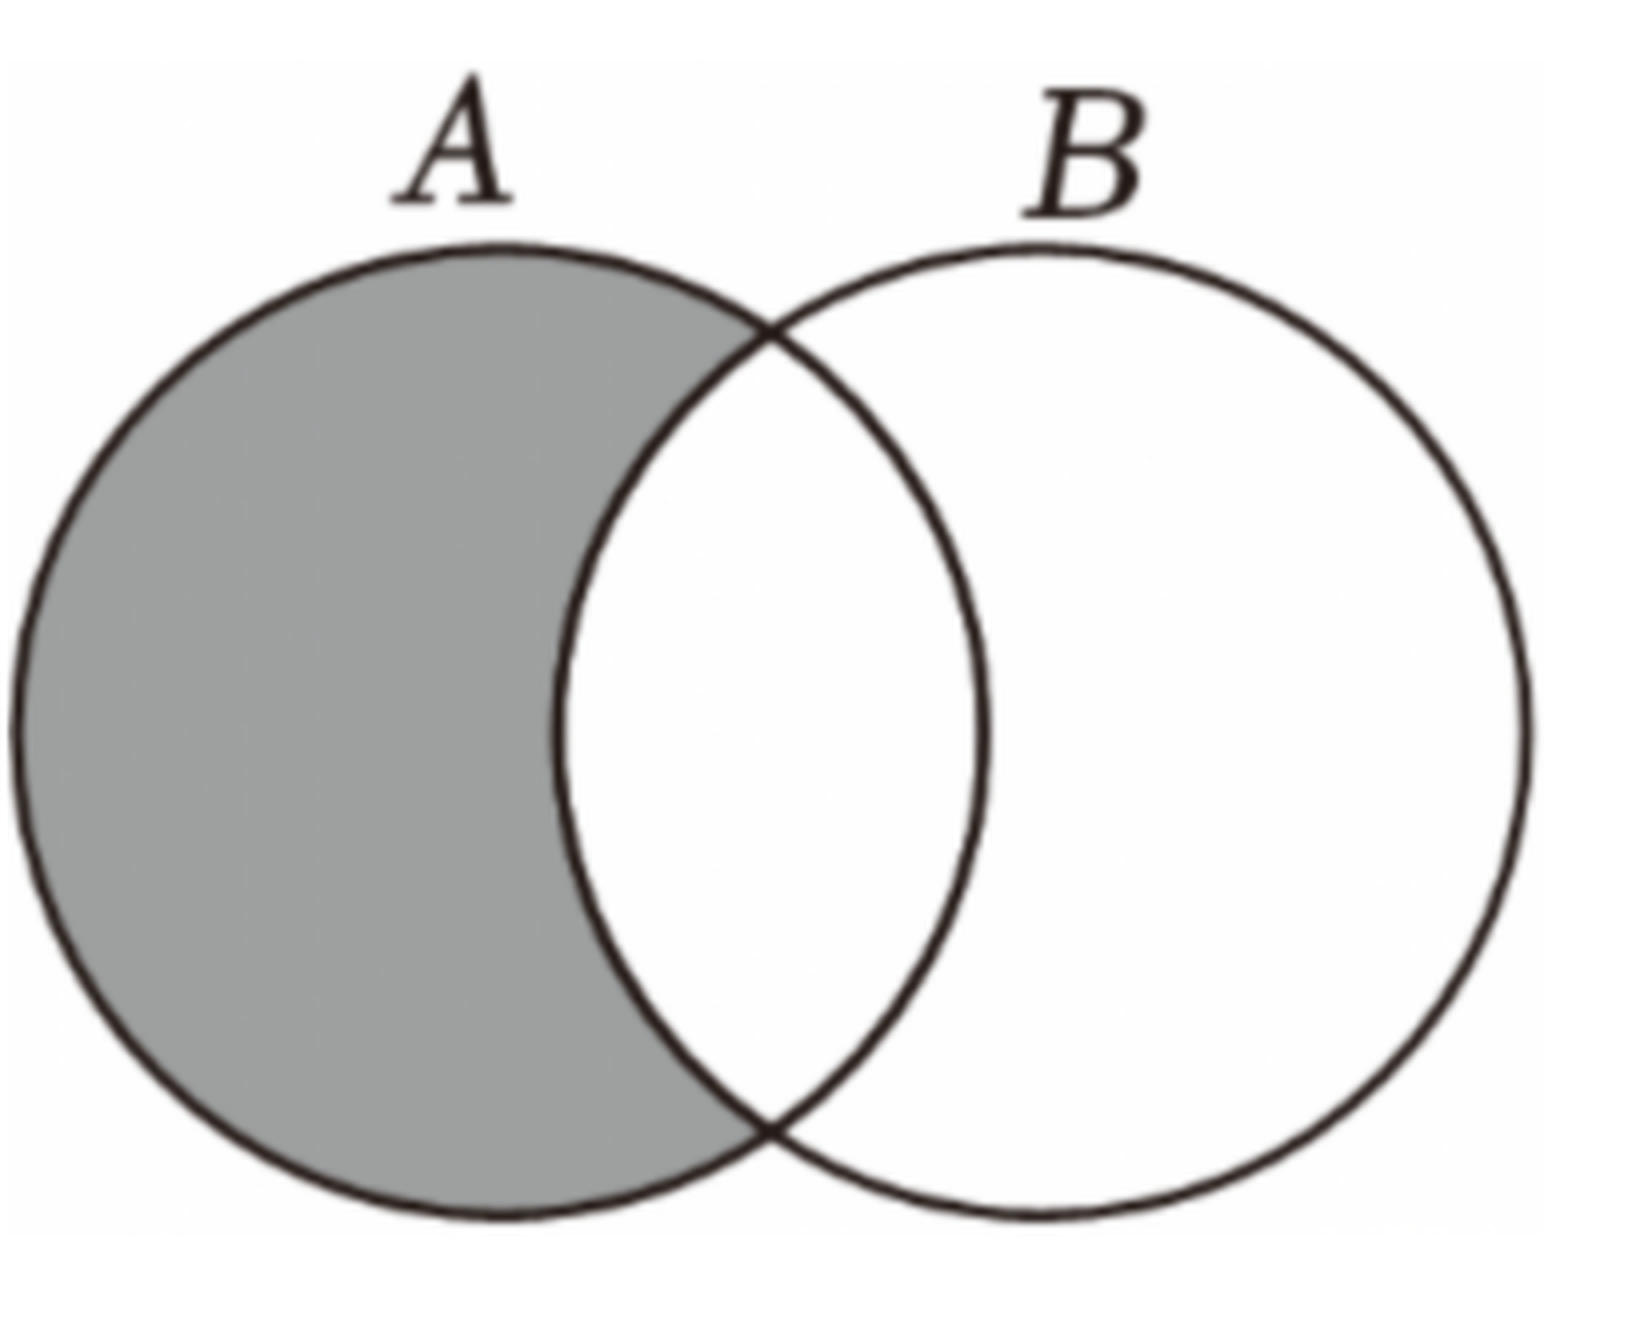
\includegraphics[width=0.30\textwidth]{figures/venn_A_minus_B_h38.png}
\end{center}

\ans{$\{1\}$}

\item 集合 $\{2,3,4,\cdots,2024,2025\}$ 的真子集的个数为 \blankline[4.4em].

\ans{$2^{2024}-1$}

\ifanswer
\solbegin
\step{集合 $\{2,3,4,\cdots,2024,2025\}$ 的真子集的个数为 $2^{2024}-1$.}
\solend

\fi

\item 已知集合 $A$ 中的元素都是正整数，其中最小的是 $1$，最大值是 $100$，除 $1$ 以外，每一个元
素都等于 $A$ 中的两个数（可以相同）的和，则集合 $A$ 中至少含有 \blankline[4.4em] 个元素.

\ans{$9$}

\ifanswer
\solbegin
\step{设 $A$ 中的数从小到大排列为 $1,a_1,a_2,\cdots,a_k,100$，}
\step{则 $a_1=1+1=2$；$3\leqslant a_2\leqslant 4$；$4\leqslant a_3\leqslant 8$；$5\leqslant a_4\leqslant 16$；$6\leqslant a_5\leqslant 32$；$7\leqslant a_6\leqslant 64$；}
\step{于是 $A$ 至少有八个数；}
\step{假设 $A$ 恰好有八个元素，由于 $a_5+a_6\leqslant 96<100$；}
\step{故必须有 $100=a_6+a_6$，$a_6=50$，}
\step{又 $a_4+a_5\leqslant 48$，同理 $a_5=25$，}
\step{但此时 $a_3+a_4\leqslant 24$，$a_5=2a_4$，$a_4=12.5$ 矛盾，}
\step{故 $A$ 不可能恰好有八个元素，因此 $A$ 至少有九个元素.}
\step{其九个数可以为 $1$，$2$，$3$，$6$，$12$，$13$，$25$，$50$，$100$.}
\solend

\fi

\item 已知集合 $\{x_1,x_2,x_3,x_4,x_5,x_6\}=\{1,2,3,4,5,6\}$，将 $x_i$ 与 $x_j$（其中 $i\in\{1,2,3\}$，
$j\in\{4,5,6\}$）的乘积 $x_ix_j$ 放入如图的 $3\times3$ 方格中，则方格中全部数之和的最大值为 \blankline[4.4em].

% 原卷的 $3\times3$ 方格是表格式内容（三行三列的公式），本稿按 高一03 的成例用 tabular 排出。
\begin{center}
\begin{tabular}{|c|c|c|}
\hline
$x_1x_4$ & $x_1x_5$ & $x_1x_6$ \\
\hline
$x_2x_4$ & $x_2x_5$ & $x_2x_6$ \\
\hline
$x_3x_4$ & $x_3x_5$ & $x_3x_6$ \\
\hline
\end{tabular}
\end{center}

\ans{$110$}

\ifanswer
\solbegin
\step{由表格数据得所有数之和为}
\step{$S=x_1x_4+x_1x_5+x_1x_6+x_2x_4+x_2x_5+x_2x_6+x_3x_4+x_3x_5+x_3x_6$，}
\step{所以 $S=(x_1+x_2+x_3)(x_4+x_5+x_6)$，}
\step{因为集合 $\{x_1,x_2,x_3,x_4,x_5,x_6\}=\{1,2,3,4,5,6\}$，}
\step{所以 $x_1+x_2+x_3+x_4+x_5+x_6=1+2+3+4+5+6=21$，}
\step{设 $t=x_1+x_2+x_3$，则 $6\leqslant t\leqslant 15$，$t\in\N^*$，}
\step{$S=t(21-t)=-\left(t-\dfrac{21}{2}\right)^2+\dfrac{441}{4}$，}
\step{当 $t=10$ 或 $t=11$ 时，$S=t(21-t)$ 取最大值，最大值为 $110$，}
\step{此时 $\{x_1,x_2,x_3\}=\{1,4,5\}$，$t=10$，所以可取最大值 $110$.}
\solend

\fi

\item 若 $[x]$ 表示不大于 $x$ 的最大整数，方程 $x^2-8[x]+7=0$ 的解集为 \blankline[4.4em].

\ans{$\{1,\sqrt{33},\sqrt{41},7\}$}

\ifanswer
\solbegin
\step{由题意，$x\geqslant[x]=\dfrac{x^2+7}{8}>0$，得 $x^2-8x+7\leqslant 0$，解得 $1\leqslant x\leqslant 7$，}
\step{$[x]=1$，$x^2=1$，$x=1$；}
\step{$[x]=2$，$x^2=9$，$x=3$ 与 $[x]=2$ 矛盾；}
\step{$[x]=3$，$x^2=17$，$x=\sqrt{17}$，$[x]=4$ 与 $[x]=3$ 矛盾；}
\step{$[x]=4$，$x^2=25$，$x=5$ 与 $[x]=4$ 矛盾；}
\step{$[x]=5$，$x^2=33$，$x=\sqrt{33}$，$[x]=5$；}
\step{$[x]=6$，$x^2=41$，$x=\sqrt{41}$，$[x]=6$；}
\step{$[x]=7$，$x^2=49$，$x=7$；}
\step{综上，方程 $x^2-8[x]+7=0$ 的解集为 $\{1,\sqrt{33},\sqrt{41},7\}$.}
\solend

\fi

\end{enumerate}

\bigsec{二、选择题}

\begin{enumerate}
\setcounter{enumi}{10}

\item 已知集合 $A=\{a,a^2\}$，$B=\{1,3\}$，若 $1\in A$，则 $A\cup B$ 中所有元素之和为\mbox{（\quad）}

\keepwithprev
A. $2$\qquad B. $3$\qquad C. $4$\qquad D. $5$

\ans{$B$}

\ifanswer
\solbegin
\step{因为 $1\in A$，集合 $A=\{a,a^2\}$，所以 $a=1$ 或 $a^2=1$，}
\step{若 $a=1$，则 $a=a^2$，与元素的互异性矛盾；}
\step{若 $a^2=1$，则 $a=1$（舍）或 $a=-1$，故 $A=\{-1,1\}$，$B=\{1,3\}$，}
\step{故 $A\cup B=\{-1,1,3\}$，所以 $A\cup B$ 中所有元素之和为 $-1+1+3=3$. 故选 $B$.}
\solend

\fi

\item 对于实数 $a$、$b$、$c$，下列命题正确的是\mbox{（\quad）}

\keepwithprev
A. 若 $a>b$，则 $ac^2>bc^2$\qquad B. 若 $a>b$，则 $a^2>b^2$

C. 若 $a>b$，则 $a|a|>b|b|$\qquad D. 若 $a>b>c>0$，则 $\dfrac{b}{a-b}<\dfrac{c}{a-c}$

\ans{$C$}

\ifanswer
\solbegin
\step{对于 $A$，若 $a>b$，$c=0$，则 $ac^2=bc^2$，故 $A$ 错误；}
\step{对于 $B$，若 $a>b$，取 $a=-1$，$b=-2$，则 $a^2<b^2$，故 $B$ 错误；}
\step{对于 $C$，若 $a>b>0$ 时，$a|a|-b|b|=a^2-b^2>0$，}
\step{当 $a>0>b$ 时，$a|a|-b|b|=a^2+b^2>0$，}
\step{当 $0>a>b$ 时，$a|a|-b|b|=b^2-a^2=(b-a)(b+a)>0$，}
\step{综上，若 $a>b$，则 $a|a|>b|b|$，故 $C$ 正确；}
\step{对于 $D$，若 $a>b>c>0$，$\dfrac{b}{a-b}-\dfrac{c}{a-c}=\dfrac{ab-bc-ac+bc}{(a-b)(a-c)}=\dfrac{a(b-c)}{(a-b)(a-c)}>0$，}
\step{故 $D$ 错误.}
\step{故选 $C$.}
\solend

\fi

\item 对于正整数集合 $A=\{a_1,a_2,\cdots,a_n\}(n\in\N^*,\ n\geqslant 3)$，如果去掉其中任意一个元素
$a_i(i=1,2,\cdots,n)$ 之后，剩余的所有元素组成的集合都能分为两个交集为空集的集合，且这
两个集合的所有元素之和相等，就称集合 $A$ 为平衡集. 记 $M=a_1+a_2+\cdots+a_n$. 若集合 $A$
是平衡集，并且存在 $a_i$ 为奇数，则集合 $A$ 中元素个数 $n$ 的奇偶性\mbox{（\quad）}

\keepwithprev
A. 与 $M$ 相关，既可以是奇数，又可以是偶数

B. 与 $M$ 无关，既可以是奇数，又可以是偶数

C. 与 $M$ 无关，必为偶数

D. 与 $M$ 无关，必为奇数

\ans{$D$}

\ifanswer
\solbegin
\step{正整数集合 $A=\{a_1,a_2,\cdots,a_n\}(n\in\N^*,\ n\geqslant 3)$，}
\step{因为集合 $A$ 是平衡集，设去掉元素 $a_i(i=1,2,\cdots,n)$，}
\step{由题意得 $A=A_1\cup A_2\cup\{a_i\}$，其中 $A_1\cap A_2=\varnothing$，}
\step{设集合 $A_1$ 和 $A_2$ 中的元素之和均为 $m$，所以 $M=2m+a_i$，其中 $i=1,2,\cdots,n$，}
\step{所以 $M-a_i=2m$，所以 $M-a_i$ 为偶数，其中 $i=1,2,\cdots,n$，}
\step{所以 $a_i(i=1,2,\cdots,n)$ 的奇偶性相同；}
\step{因为存在 $a_i$ 为奇数，所以 $a_i(i=1,2,\cdots,n)$ 均为奇数，}
\step{由 $M-a_i=2m$ 得 $M$ 也为奇数，且 $M=a_1+a_2+\cdots+a_n$，}
\step{所以 $n$ 也为奇数，所以 $n$ 必为奇数. 故选 $D$.}
\solend

\fi

\item 对于集合 $M=\{a\mid a=x^2-y^2,\ x\in\Z,\ y\in\Z\}$，给出如下三个结论：其中正确结论的个数
是\mbox{（\quad）}

\keepwithprev
①如果 $P=\{b\mid b=2n+1,\ n\in\Z\}$，那么 $P\sub M$；

②如果 $c=4n+2$，$n\in\Z$，那么 $c\notin M$；

③如果 $a_1\in M$，$a_2\in M$，那么 $a_1a_2\in M$.

\keepwithprev
A. $1$\qquad B. $2$\qquad C. $3$\qquad D. $0$

\ans{$C$}

\ifanswer
\solbegin
\step{对于①，$b=2n+1$，$n\in\Z$，则恒有 $2n+1=(n+1)^2-n^2$，}
\step{所以 $2n+1\in M$，即 $P=\{b\mid b=2n+1,n\in\Z\}$，则 $P\sub M$，①正确；}
\step{对于②，$c=4n+2$，$n\in\Z$，}
\step{若 $4n+2\in M$，则存在 $x$、$y\in\Z$ 使得 $x^2-y^2=4n+2$，}
\step{所以 $4n+2=(x+y)(x-y)$，又 $x+y$ 和 $x-y$ 同奇或同偶，}
\step{若 $x+y$ 和 $x-y$ 都是奇数，则 $(x+y)(x-y)$ 为奇数，而 $4n+2$ 是偶数；}
\step{若 $x+y$ 和 $x-y$ 都是偶数，则 $(x+y)(x-y)$ 能被 $4$ 整除，而 $4n+2$ 不能被 $4$ 整除，}
\step{所以 $4n+2\notin M$，即 $c\notin M$，②正确；}
\step{对于③，$a_1\in M$，$a_2\in M$，可设 $a_1=x_1^2-y_1^2$，$a_2=x_2^2-y_2^2$，$x_i$、$y_i\in\Z$；}
\step{则 $a_1a_2=(x_1^2-y_1^2)(x_2^2-y_2^2)=(x_1x_2)^2+(y_1y_2)^2-(x_1y_2)^2-(x_2y_1)^2$}
\step{$=(x_1x_2+y_1y_2)^2-(x_1y_2+x_2y_1)^2\in M$，那么 $a_1a_2\in M$，③正确.}
\step{综上，正确的命题是①②③. 故选 $C$.}
\solend

\fi

\end{enumerate}

\bigsec{三、解答题}

\begin{enumerate}
\setcounter{enumi}{14}

\item 已知 $A=\{x\mid a\leqslant x\leqslant -a+3\}$，$B=\{x\mid x<-1\text{ 或 }x>5\}$.

\begin{enumerate}[label=(\arabic*)]

\item 若 $A\cap B=\varnothing$，求 $a$ 的取值范围；

\item 若 $A\cup B=\R$，求 $a$ 的取值范围.

\end{enumerate}

\ans{（1）$[-1,+\infty)$；（2）$(-\infty,-2]$}

\ifanswer
\solbegin
\stepm{(1)}{①当 $A=\varnothing$ 时，$A\cap B=\varnothing$，需满足 $a>-a+3$，解得 $a>\dfrac32$，}
\step{故 $a$ 的取值范围为 $\left(\dfrac32,+\infty\right)$.}
\step{②当 $A\neq\varnothing$ 时，要使 $A\cap B=\varnothing$，需满足
$\begin{cases}a\leqslant\dfrac32\\[4pt] -a+3\leqslant 5\\[4pt] a\geqslant -1\end{cases}$，解得 $-1\leqslant a\leqslant\dfrac32$.}
\step{综上所述，$a$ 的取值范围是 $[-1,+\infty)$.}
\stepm{(2)}{因为 $A\cup B=\R$，$A=\{x\mid a\leqslant x\leqslant -a+3\}$，$B=\{x\mid x<-1\text{ 或 }x>5\}$，}
\step{所以 $\begin{cases}-a+3\geqslant 5\\[4pt] a\leqslant -1\end{cases}$，解得 $a\leqslant -2$，故所求 $a$ 的取值范围为 $(-\infty,-2]$.}
\solend

\fi

\ansspace[6]

\item 已知集合 $A=\{x\mid mx^2+x-2=0\}$，$B=\{x\mid 2x^2-5x-12=0\}$.

\begin{enumerate}[label=(\arabic*)]

\item 若 $A$ 中有且仅有 $1$ 个元素，求实数 $m$ 的值；

\item 已知集合 $C=A\cup B$，若 $C$ 的真子集有且仅有 $3$ 个，求实数 $m$ 的取值范围.

\end{enumerate}

\ans{（1）$m=0$ 或 $m=-\dfrac18$；（2）$\left\{m\mid m\leqslant -\dfrac18\right\}$}

\ifanswer
\solbegin
\stepm{(1)}{若 $m=0$，方程化为 $x-2=0$，此时方程有且仅有一个根 $x=2$；}
\step{若 $m\neq 0$，则 $\Delta=1^2-4\times m\times(-2)=0$，即 $m=-\dfrac18$ 时，}
\step{方程有两个相等的实根，此时集合 $A$ 中有且仅有一个元素，}
\step{所以实数 $m$ 的值为 $m=0$ 或 $m=-\dfrac18$；}
\stepm{(2)}{$B=\{x\mid 2x^2-5x-12=0\}=\left\{-\dfrac32,4\right\}$，}
\step{因为 $C=A\cup B$，若 $C$ 的真子集有且仅有 $3$ 个，则 $C$ 中有两个元素，}
\step{所以 $A\sub B$，由（1）得 $m=0$ 时，$A=\{2\}$，不符合 $A\sub B$，}
\step{当 $m\neq 0$ 时，若 $\Delta=1^2-4\times m\times(-2)<0$，解得 $m<-\dfrac18$，}
\step{此时 $A=\varnothing$，符合 $A\sub B$，}
\step{若 $\Delta=1^2-4\times m\times(-2)=0$，解得 $m=-\dfrac18$，}
\step{此时方程 $mx^2+x-2=0$ 的根为 $x=4$，集合 $A=\{4\}$，符合 $A\sub B$，}
\step{若 $\Delta=1^2-4\times m\times(-2)>0$，由 $A\sub B$，得 $A=\left\{-\dfrac32,4\right\}$，}
\step{此时有 $-\dfrac32+4=-\dfrac1m$ 且 $-\dfrac32\times 4=-\dfrac2m$，无解，}
\step{综上所述，实数 $m$ 的取值范围为 $\left\{m\mid m\leqslant -\dfrac18\right\}$.}
\solend

\fi

\ansspace[6]

\item 设 $A$ 是非空实数集，且 $0\notin A$. 若对于任意的 $x$、$y\in A$，都有 $xy\in A$，则称集合 $A$ 具
有性质 $P_1$；若对于任意的 $x$、$y\in A$，都有 $\dfrac xy\in A$，则称集合 $A$ 具有性质 $P_2$.

\begin{enumerate}[label=(\arabic*)]

\item 写出一个恰含有两个元素且具有性质 $P_1$ 的集合 $A$，并说明理由；

\item 证明：“非空实数集 $A$ 具有性质 $P_1$”是“非空实数集 $A$ 具有性质 $P_2$”的必要非充分条
件.

\end{enumerate}

\ans{（1）$A=\{-1,1\}$，理由见解析；（2）见解析}

\ifanswer
\solbegin
% 注：原卷本题 (1) 的解析里“证明”一词重复出现两次（一次接在分号后、一次另起一行），
%     本稿照原卷重复录入，未去重。
\stepm{(1)}{$A=\{-1,1\}$，证明：恰含有两个元素且具有性质 $P_1$ 的集合 $A=\{-1,1\}$；}
\step{证明：$1\times 1=1\in A$，$1\times(-1)=-1\in A$，$-1\times 1=-1\in A$，$-1\times(-1)=1\in A$；}
\stepm{(2)}{若集合 $A$ 具有性质 $P_2$，不妨设 $a\in A$，}
\step{由非空数集 $A$ 具有性质 $P_2$，有 $\dfrac aa=1\in A$.}
\step{①$A=\{1\}$，易得此时集合 $A$ 具有性质 $P_1$.}
\step{②数集 $A$ 只含有两个元素，不妨设 $A=\{1,a_1\}$，}
\step{由 $\dfrac{1}{a_1}=a_1$，且 $a_1\neq 1$，解得 $a_1=-1$，此时集合 $A$ 具有性质 $P_1$.}
\step{③实数集 $A$ 含有两个以上的元素，不妨设不为 $1$ 的元素 $a_1$、$a_2\in A$，}
\step{则有 $\dfrac{1}{a_1}\in A$，由于集合 $A$ 具有性质 $P_2$，}
\step{所以有 $a_2\div\dfrac{1}{a_1}=a_1a_2\in A$，这说明集合 $A$ 具有性质 $P_1$.}
\step{综上，若非空实数集 $A$ 具有性质 $P_2$，则集合 $A$ 具有性质 $P_1$，}
\step{所以“非空实数集 $A$ 具有性质 $P_1$”是“非空实数集 $A$ 具有性质 $P_2$”的}
\step{必要条件.}
\step{取正偶数集 $A=\{x\mid x=2n,\ n\in\N^*\}$，}
\step{对任意的 $2m$、$2n\in A$，$m$、$n\in\N^*$，}
\step{有 $2m\times 2n=4mn\in A$，故 $A$ 具有性质 $P_1$，}
\step{取 $x=2$，$y=4$，则 $\dfrac xy=\dfrac12\notin A$，故 $A$ 不具有性质 $P_2$，}
\step{所以“非空实数集 $A$ 具有性质 $P_1$”不是“非空实数集 $A$ 具有性质 $P_2$”的}
\step{充分条件.}
\step{综上，“非空实数集 $A$ 具有性质 $P_1$”是“非空实数集 $A$ 具有性质 $P_2$”的}
\step{必要非充分条件.}
\solend

\fi

\ansspace[8]

\item 已知命题 $p$：关于 $x$ 的方程 $x^2+mx+1=0$ 有两个不同的正根；命题 $q$：关于 $x$ 的方程
$4x^2+4(m-2)x=-1$ 有实根.

\begin{enumerate}[label=(\arabic*)]

\item 若命题 $q$ 为假命题，求整数 $m$ 的解集；

\item 若命题 $p$ 为真命题，且关于 $x$ 的方程 $x^2+mx+1=0$ 的两个实数根 $x_1$、$x_2$ 满足
$3x_1+2x_2=5$，求实数 $m$ 的取值集合；

\item 若命题 $p$ 和命题 $q$ 有且仅有一个成立，求实数 $m$ 的取值范围.

\end{enumerate}

\ans{（1）$\{2\}$；（2）$\left\{-\dfrac{13}{6}\right\}$；（3）$[-2,1]\cup[3,+\infty)$}

\ifanswer
\solbegin
\stepm{(1)}{命题 $q$：关于 $x$ 的方程 $4x^2+4(m-2)x=-1$ 有实根为假命题，}
\step{即 $4x^2+4(m-2)x+1=0$ 无实根，}
\step{则 $\Delta=16(m-2)^2-16<0$，则 $1<m<3$，则整数 $m$ 的解集为 $\{2\}$；}
\stepm{(2)}{若命题 $p$ 为真命题，且关于 $x$ 的方程 $x^2+mx+1=0$ 的两个实数根 $x_1$、$x_2$，}
\step{满足 $3x_1+2x_2=5$，则方程 $x^2+mx+1=0$ 有两个不同的正根，}
\step{则 $\begin{cases}\Delta=m^2-4>0\\[4pt] x_1+x_2=-m>0\end{cases}$，则 $m<-2$，}
\step{又 $\begin{cases}x_1+x_2=-m\\[4pt] x_1x_2=1\\[4pt] 3x_1+2x_2=5\end{cases}$，
则 $\begin{cases}x_1=5+2m\\[4pt] x_2=-3m-5\end{cases}$，则 $(5+2m)(-3m-5)=1$，}
\step{得 $m=-2$ 或 $m=-\dfrac{13}{6}$，又因为 $m<-2$，所以 $m=-\dfrac{13}{6}$，}
\step{所以实数 $m$ 的取值集合为 $\left\{-\dfrac{13}{6}\right\}$；}
\stepm{(3)}{由（2）得当 $p$ 为真时，则有 $m<-2$，}
\step{当 $q$ 为真时，$\Delta=16(m-2)^2-16\geqslant 0$，解得 $m\leqslant 1$ 或 $m\geqslant 3$，}
\step{又因为命题 $p$ 和命题 $q$ 只有一个为真，所以
$\begin{cases}m<-2\\[4pt] 1<m<3\end{cases}$ 或 $\begin{cases}m\geqslant -2\\[4pt] m\leqslant 1\text{ 或 }m\geqslant 3\end{cases}$，}
\step{解得 $-2\leqslant m\leqslant 1$ 或 $m\geqslant 3$，所以实数 $m$ 的取值范围为 $[-2,1]\cup[3,+\infty)$.}
\solend

\fi

\ansspace[8]

% 注：原卷此处作“设 $n\in\N^*$，集合含有 $3n$ 个元素”，**漏了符号 $U$**（应作“集合 $U$
%     含有 $3n$ 个元素”）——$U$ 直到本句末尾“则称 $U$ 为三分集合”才出现、此前无定义。
%     本稿照录未补，见文件头“原卷笔误/存疑”⑦。
\item 设 $n\in\N^*$，集合含有 $3n$ 个元素，若存在三个 $n$ 元集合 $A$、$B$、$C$ 满足如下两个条件，
则称 $U$ 为三分集合.

①$U=A\cup B\cup C$；

②$A$、$B$、$C$ 元素可分别排列为有序数组 $(a_1,a_2,\cdots,a_n)$，$(b_1,b_2,\cdots,b_n)$ 及
$(c_1,c_2,\cdots,c_n)$，使得对 $\forall i=1,2,\cdots,n$，均有 $a_i+b_i=c_i$.

特别地，当 $U=\{1,2,3,4,\cdots,3n-2,3n-1,3n\}$ 为三分集合时，称 $n$ 为完美三分数.

如：因为 $U=\{1,2,3\}$ 为三分集合，所以 $n=1$ 为最小完美三分数.

\begin{enumerate}[label=(\arabic*)]

\item 请判断下列两个集合是否为三分集合（直接写出结论）：

$U_1=\{1,2,3,4,5,6\}$，$U_2=\{1,3,5,7,8,9,10,11,12\}$；

\item 求出大于 $1$ 的最小完美三分数；

\item 请判断是否存在无穷多个完美三分数？若存在，请说明理由；若不存在，则求出最大的
完美三分数.

\end{enumerate}

\ans{（1）$U_1$ 不是三分集合，$U_2$ 是三分集合；（2）$4$；（3）存在，理由见解析}

\ifanswer
\solbegin
\stepm{(1)}{(i)$U_1=\{1,2,3,4,5,6\}$ 不是三分集合，下面用反证法证明：}
\step{证明：假设 $U=\{1,2,3,4,5,6\}$ 是三分集合，}
\step{设 $A=\{a_1,a_2\}$，$B=\{b_1,b_2\}$，$C=\{c_1,c_2\}$，不妨设 $c_1<c_2$，}
\step{因为 $a_1+b_1=c_1$，$a_2+b_2=c_2$，}
\step{所以 $a_1+b_1+a_2+b_2+c_1+c_2=2(c_1+c_2)=1+2+3+4+5+6=21$，}
% 注：原卷此步印“所以 $c_1+c_2=2$”，与上一行的 $2(c_1+c_2)=21$ **不自洽**
%     （应作 $\dfrac{21}2$）；同题 $n=3$ 处的同型推理原卷写的是 $\dfrac{45}2$，故此处是原卷笔误。
%     本稿照录未改，见文件头“原卷笔误/存疑”⑧。
\step{所以 $c_1+c_2=2$，这与 $c_1,c_2\in\N^*$ 矛盾，故假设错误，}
\step{故 $U_1=\{1,2,3,4,5,6\}$ 不是三分集合；}
\step{(ii)$U_2=\{1,3,5,7,8,9,10,11,12\}$ 是三分集合，理由如下：}
\step{令 $A=\{1,3,5\}$，$B=\{9,8,7\}$，$C=\{10,11,12\}$，}
\step{则 $A\cup B\cup C=U=\{1,3,5,7,8,9,10,11,12\}$，满足条件①；}
\step{又 $1+9=10$；$3+8=11$；$5+7=12$，所以满足条件②，}
\step{所以 $U_2=\{1,3,5,7,8,9,10,11,12\}$ 是三分集合；}
\stepm{(2)}{由（1）得，当 $n=2$ 时，$U=\{1,2,3,4,5,6\}$ 不是三分集合；}
\step{当 $n=3$ 时，$U=\{1,2,3,4,5,6,7,8,9\}$，}
\step{假设 $U=\{1,2,3,4,5,6,7,8,9\}$ 是三分集合，}
\step{同理由 $a_1+b_1+a_2+b_2+a_3+b_3+c_1+c_2+c_3$}
\step{$=2(c_1+c_2+c_3)=1+2+\cdots+9=45$，$c_1+c_2+c_3=\dfrac{45}{2}$，}
\step{可推出与 $c_1$、$c_2$、$c_3\in\N^*$ 矛盾，故假设也错误，}
\step{所以 $U=\{1,2,3,4,5,6,7,8,9\}$ 不是三分集合；}
\step{当 $n=4$ 时，$U=\{1,2,3,\cdots,12\}$，}
\step{存在三个 $4$ 元集合 $A=\{1,2,4,3\}$，$B=\{5,8,7,9\}$，$C=\{6,10,11,12\}$，}
\step{满足 $U=\{1,2,3,\cdots,12\}$ 为三分集合的两个条件，}
\step{故大于 $1$ 的最小完美三分数为 $4$；}
\stepm{(3)}{存在无穷多个完美三分数，理由如下：}
\step{由题意得，$n=1$ 为最小完美三分数，}
\step{当 $n=5$ 时，$U=\{1,2,3,\cdots,15\}$，}
\step{存在三个 $5$ 元集合 $A=\{1,3,5,7,2\}$，$B=\{11,10,9,8,4\}$，$C=\{12,13,14,15,6\}$，}
\step{满足三分集合的条件，故 $5$ 为完美三分数；}
\step{当 $n=21$ 时，$U=\{1,2,3,\cdots,63\}$，}
\step{存在如下三个 $21$ 元的集合满足三分集合的条件：}
\step{$A=\{1,3,5,7,\cdots,29,31,2,6,10,14,4\}$，}
\step{$B=\{47,46,45,44,\cdots,33,32,22,20,18,16,8\}$，}
\step{$C=\{48,49,50,51,\cdots,62,63,24,26,28,30,12\}$，}
\step{故 $21$ 为完美三分数.}
\step{首先证明：若 $n=k$，$k\in\N^*$ 为三分完美数，}
\step{则 $n=4k+1$，$k\in\N^*$ 也为三分完美数，}
% 注：下一行原卷印作“$U_{k+1}=U_{k+1}=\{2,3,\cdots,12k+3\}$”——等号两边记号相同，
%     依上下文疑当作 $U'_{k+1}=U_{4k+1}$，且此处集合自 2 起（前文 $U_{4k+1}$ 自 1 起）；
%     本稿照录原卷，未代为改写。
\step{证明：记 $U_k=\{1,2,3,\cdots,3k\}$，$U_{4k+1}=\{1,2,3,\cdots,12k+3\}$，}
\step{若 $n=k$，$k\in\N^*$ 为三分完美数，则 $U_k$ 为三分集合，}
\step{即存在三个 $k$ 元集合 $A$、$B$、$C$ 满足如下两个条件，}
\step{①$U_k=A\cup B\cup C$；}
\step{②$A$、$B$、$C$ 元素可分别排列为有序数组 $(a_1,a_2,\cdots,a_k)$，}
\step{$(b_1,b_2,\cdots,b_k)$ 及 $(c_1,c_2,\cdots,c_k)$，}
\step{使得对 $\forall i=1,2,3,\cdots,k$，均有 $a_i+b_i=c_i$，}
\step{则可得到对 $\forall i=1,2,3,\cdots,k$，$2a_i+2b_i=2c_i$，}
\step{故集合 $\{2,4,6,\cdots,6k\}$ 也满足三分集合的两个条件，其也为三分集合，}
\step{下面记集合 $\{2,4,6,\cdots,6k\}=2U_k$，}
\step{对 $n=4k+1$，集合 $U_{k+1}=U_{k+1}=\{2,3,\cdots,12k+3\}=(2U_k)\cup\complement_{U_{4k+1}}(2U_k)$，}
\step{构造集合 $A'=\{1,3,5,7,\cdots,6k+1\}$，共有 $3k+1$ 个奇数；}
% 注：下一行原卷印作“$B'=\{6k+3k+2,6k+3k+1,6k+3k,6k+3k-1,\cdots,6k+2\}$”，
%     按与后文 $C'$ 相接，前四项当写作 $9k+2$、$9k+1$、$9k$、$9k-1$；本稿照录原卷。
\step{集合 $B'=\{6k+3k+2,6k+3k+1,6k+3k,6k+3k-1,\cdots,6k+2\}$，}
\step{共有 $3k+1$ 个逐个减小的连续正整数；}
\step{集合 $C'=\{9k+3,9k+4,9k+5,9k+6,\cdots,12k+3\}$，}
\step{共有 $3k+1$ 个逐个增大的连续正整数；}
\step{得这三个 $3k+1$ 元集合 $A'$、$B'$、$C'$ 满足如下两个条件，}
\step{①集合 $A'\cup B'\cup C'=\complement_{U_{4k+1}}(2U_k)$；}
\step{②$A'$、$B'$、$C'$ 元素可分别排列为有序数组 $(a_1,a_2,\cdots,a_{3k+1})$，}
\step{$(b_1,b_2,\cdots,b_{3k+1})$ 及 $(c_1,c_2,\cdots,c_{3k+1})$，}
\step{使得对 $\forall i=1,2,3,\cdots,3k+1$，均有 $a_i+b_i=c_i$；}
\step{故 $\complement_{U_{4k+1}}(2U_k)$ 为三分集合，而已知 $U_k$ 为三分集合，}
\step{将其对应与 $A'$、$B'$、$C'$ 合并，}
% 注：原卷此处印“令 $A''=A\cup A'$”（$B''$、$C''$ 同）。按同段上文“记集合
%     $\{2,4,6,\cdots,6k\}=2U_k$”，此处疑当作 $A''=2A\cup A'$——否则
%     $A''\cup B''\cup C''=U_k\cup\complement_{U_{4k+1}}(2U_k)\neq U_{4k+1}$，与本段结论冲突。
%     本稿照录未改，见文件头“原卷笔误/存疑”⑨。
\step{令 $A''=A\cup A'$，$B''=B\cup B'$，$C''=C\cup C'$，}
\step{则这三个 $4k+1$ 元集合 $A''$、$B''$、$C''$，}
\step{满足 $A''\cup B''\cup C''=U_{4k+1}$，且满足条件②，}
\step{故 $U_{4k+1}=\{1,2,3,\cdots,12k+3\}$ 为三分集合，}
\step{因此可得，若 $n=k$ 为三分完美数，则 $n=4k+1$ 也为三分完美数，}
\step{由 $1$，$5$，$21$ 为完美三分数，结合所证结论得，存在无穷多个完美三分数.}
\solend

\fi

\ansspace*[12]

\end{enumerate}

\end{document}
"
%
% 原始材料是微信公众号图文（公众号“魔都数学加油站”连载“27学年高一 38”，署名“破晓”，
% 2026-09-26 21:29 发布，原文标题“27学年高一38——2026-2027年上海市大同中学高一上周末作业3”，
% 原文链接 https://mp.weixin.qq.com/s/O_O60vCIiGi2xponAo4irw ），正文为 12 张 PNG 页。
% **同一篇里各页分辨率不一致**（2560×3620 与 4762×6735 两档混排：第 1、10、11、12 页为
% 2560×3620，第 2—9 页为 4762×6735）。原文本身就是一份**讲评版**——有的题下方只印
% 【答案】行，有的只印【解析】。试题文字、答案与解析均照原卷录入，未改内容。卷面的粉色
% 斜水印“魔都数学加油站”属水印，未录入。
%
% 本卷共 **17 题**：填空题 8 题（第 3—10 题）、选择题 4 题（第 11—14 题）、解答题 5 题
% （第 15—19 题）；插图 1 张（第 6 题 Venn 图）。三版页数：试卷版 4 页 / 答案版 11 页 /
% 紧凑版 3 页，`Overfull`／`Underfull`／`Missing character` 告警均为 0。
%
% 卷首标题：原卷印作“2026-2027 年大同中学高一上周末作业 3”（公众号原文标题里的“上海市”
% 三字卷面标题行没有，本稿照卷面），年份区间按全稿惯例排 en dash，前缀照原卷保留“年”。
%
% 与原卷的排版差异（均已在 README“说明”中交代）：
%   ① 原文自**第 3 题**起（第 1、2 题未在该文中发布），故本稿题号亦自 3 起，填空题以
%      \setcounter{enumi}{2} 起编；选择、解答两节各按上一节末号另设 \setcounter
%      （选择题 \setcounter{enumi}{10}、解答题 \setcounter{enumi}{14}）；
%   ② 原卷本就印有“一、填空题”“二、选择题”“三、解答题”三节标题，本稿照原卷分节，
%      只把标题改排成全稿统一的“大节标题”样式；
%   ③ 原卷是“讲评版”：第 3、6 题只印【答案】行，第 4、5、7、8、9、10 题与第 11—19 题印
%      【解析】；本稿统一改为试卷版隐去、答案版以 \ans{}／\ifanswer 块给出，两版彻底分离。
%      其中第 4、5、7、8、9、10 题与第 11—14 题的答案，原卷写在【解析】末句，本稿另提为
%      \ans{}；第 15—19 题原卷只有【解析】、无独立答案行，本稿亦补了摘要式 \ans{}。
%      **故本卷 17 题每题都有 \ans**——比“只印【解析】的填空、解答题不另提 \ans”的
%      高一31／高一34 更彻底，与 高一21 第 11 题（填空，答案在【解析】末句，本稿另提）同类；
%      （本仓对“另提 \ans{}”的做法各卷不一，见 README 对应专记的核对面。）
%   ④ 数集记号原卷两套并用：第 3、5 题的实数集作粗体 $\mathbf{R}$，第 8、14、17、18 题等的
%      整数集、自然数集作斜体 $Z$、$N$，本稿按全稿惯例统一写作 $\R$、$\Z$、$\N$；
%   ⑤ 原卷填空的横线宽度不一（约 1.8—3.6 字宽），本稿按全稿惯例统一排 \blankline[4.4em]；
%   ⑥ 中文括注原卷用半角“(  )”，本稿按全稿惯例排全角；选择题的作答括注统一排
%      \mbox{（\quad）}（第 14 题的作答括注原卷印在 ①②③ 三个命题**之前**，本稿照原卷次序）；
%      数学式内部的括注（如第 4 题的 $p\%(0<p<100)$、第 13 题的 $a_i(i=1,2,\cdots,n)$）照原样
%      留在行内公式里，未改全角；
%   ⑦ 原卷并列的字母（“x,y”“a,b,c”）不加标点或作半角逗号，本稿按全稿惯例改排顿号；
%   ⑧ 第 6 题的 Venn 图取原卷截图、4× LANCZOS 放大（figures/venn_A_minus_B_h38.png，
%      见该处 \includegraphics 前的注释）；第 9 题的 $3\times3$ 方格属**表格式**内容，
%      本稿按 高一03 的成例用 tabular 排出，未截图；
%   ⑨ 原卷未印副标题，本稿按**本卷实际内容**补出副标题“集合与常用逻辑用语”（依据见下条）；
%   ⑩ 原卷【解析】**一个印刷行照录为一条 `\step`**（原卷的折行也照录为独立一条，如第 17 题
%      末三处“…的”／“必要条件.”这类跨行句、第 9 题“由表格数据得所有数之和为”／
%      “$S=\cdots$，”），使答案版的排布与原卷讲评版逐行对应；全卷 15 处【解析】合计
%      **191 条 `\step` ＝ 原卷 191 行**（逐处：5、5、1、9、9、9、4、9、9、12、6、14、21、13、65）。
%
% 副标题（\examtitlest 第二个参数）：本卷卷面未印副标题，由本稿补出，取值按 2026-09-26 起的
%   新口径“只用本卷实际内容的模块名”定为“集合与常用逻辑用语”。依据：全卷 17 题
%   （第 3—19 题）中，第 3、5、6、7、8、9、10、11、13、14、15、16、17、18、19 题共 15 题
%   是集合的运算与关系、子集计数、集合新定义（性质 $P_1$／$P_2$、平衡集、三分集合），以及
%   命题与逻辑（第 3 题即用反证法证明“$x+y>2\Rightarrow x>1$ 或 $y>1$”这一命题）；不等式只
%   出现在第 4 题（降价提价的应用比较）、第 12 题（不等式命题真假）与第 10 题解析里解一元
%   二次不等式，合计不足全卷的三分之一，故不并标“不等式”。
%
% 原卷笔误/存疑（均照抄原卷、未改，见源码中该处上方注释）：
%   ① 第 19 题 (3) 的证明里印作“集合 $U_{k+1}=U_{k+1}=\{2,3,\cdots,12k+3\}$”——等号两边
%      记号相同（依上下文疑当作 $U'_{k+1}=U_{4k+1}$），且此处集合自 $2$ 起，而前文
%      $U_{4k+1}=\{1,2,3,\cdots,12k+3\}$ 自 $1$ 起；本稿照录；
%   ② 第 19 题 (3) 的证明里印作
%      “$B'=\{6k+3k+2,6k+3k+1,6k+3k,6k+3k-1,\cdots,6k+2\}$”——按与后文
%      $C'=\{9k+3,9k+4,9k+5,9k+6,\cdots,12k+3\}$ 相接，前四项当写作 $9k+2$、$9k+1$、
%      $9k$、$9k-1$（即 $6k+3k+2$ 等），原卷即作“$6k+3k+\cdots$”形式，本稿照录；
%   ③ 第 19 题的术语前后不一：题干与 (1)(2)(3) 用“完美三分数”，而 (3) 的证明里五次写作
%      “三分完美数”（词序不同）；本稿五处都照录；
%   ④ 第 14 题题干作“给出如下三个结论：其中正确结论的个数是（\quad）”，此处冒号疑当作
%      逗号，本稿照录；
%   ⑤ 第 17 题题干作“非空实数集”，其解析有一处写作“非空数集”；本稿照录；
%   ⑥ 第 17 题 (1) 的【解析】原卷连写“…集合 $A=\{-1,1\}$；证明：…；证明：…”，“证明”
%      一词重复出现两次（第一次在分行处、第二次另起一行），本稿照原卷重复录入，未去重。
%   ⑦ 第 19 题**题干漏字**：原卷作“19.设 $n\in\N^*$，集合含有 $3n$ 个元素…则称 $U$ 为
%      三分集合”——首句漏了符号 $U$（应作“集合 $U$ 含有 $3n$ 个元素”），$U$ 直到结论句
%      才出现、此前无定义；本稿照录未补（见该处上方注释）。
%   ⑧ 第 19(1)(i) 的【解析】**自相矛盾**：上一行印“$a_1+b_1+a_2+b_2+c_1+c_2=2(c_1+c_2)
%      =1+2+3+4+5+6=21$”，下一行却印“所以 $c_1+c_2=2$”（由 $2(c_1+c_2)=21$ 应得
%      $c_1+c_2=\dfrac{21}2$，非整数、才与 $c_1,c_2\in\N^*$ 矛盾）；同题 $n=3$ 处的同型
%      推理原卷就写对了（$\dfrac{45}2$），故此处是原卷笔误；本稿照录未改（见该处上方注释）。
%   ⑨ 第 19(3) 的【解析】印“令 $A''=A\cup A'$，$B''=B\cup B'$，$C''=C\cup C'$”——按同段
%      上文“记集合 $\{2,4,6,\cdots,6k\}=2U_k$”，$A''$ 等疑当作 $2A\cup A'$（$B''$、$C''$ 同），
%      否则 $A''\cup B''\cup C''=U_k\cup\complement_{U_{4k+1}}(2U_k)\neq U_{4k+1}$；本稿照录未改
%      （见该处上方注释）。

\documentclass[a4paper,11pt]{article}
\usepackage{common}

\begin{document}

\examtitlest[3]{2026--2027 年大同中学高一上周末作业 3}{集合与常用逻辑用语}

\bigsec{一、填空题}

\begin{enumerate}
% 原卷填空题自第 3 题起（第 1、2 题未在该文中发布），须与选择、解答两节的 \setcounter 对齐
\setcounter{enumi}{2}

\item 设 $x$、$y\in\R$，若 $x+y>2$，则 $x>1$ 或 $y>1$ 是真命题. 这个命题可以用反证法去证明，
可以假设：\blankline[4.4em].

\ans{$x\leqslant 1$ 且 $y\leqslant 1$}

\item 已知某商品的原价为 $a$ 元，由于市场原因，先降价 $p\%(0<p<100)$ 出售，一段时间后，
再提价 $p\%$ 出售，则该商品提价后的售价 \blankline[4.4em] 该商品的原价（填“高于”“低于”或“等于”）.

\ans{低于}

\ifanswer
\solbegin
\step{由题意得第一次降价后的售价为 $a(1-p\%)$ 元，}
\step{第二次提价后的售价为 $a(1-p\%)(1+p\%)$ 元，}
\step{因为 $0<p<100$，所以 $0<p\%<1$，}
\step{因为 $a(1-p\%)(1+p\%)=a[1-(p\%)^2]<a$，}
\step{即该商品提价后的售价低于该商品的原价.}
\solend

\fi

\item 若集合 $A=\{x\mid ax^2+ax+1=0,\ a\in\R,\ x\in\R\}$ 的子集只有两个，则实数 $a=$ \blankline[4.4em].

\ans{$4$}

\ifanswer
\solbegin
\step{集合 $A=\{x\mid ax^2+ax+1=0\}$ 的子集只有两个，}
\step{所以 $A$ 有且只有一个元素，}
\step{①若 $a=0$，则 $A=\varnothing$ 不成立；}
\step{②若 $a\neq 0$，则 $\Delta=a^2-4a=0$，解得 $a=4$（$0$ 舍）.}
\step{故 $a=4$.}
\solend

\fi

\item 如图，已知集合 $A=\{1,2,3,4,5\}$，集合 $B=\{2,3,4,5,9\}$，则图中阴影部分所表示的
集合为 \blankline[4.4em].

% 图取原卷截图（01.png，2560×3620）右栏，4× LANCZOS 放大；为避免与 高一11 的
% figures/venn_A_minus_B.png 同名，按 高一32 的成例加 _h38 后缀。
\begin{center}
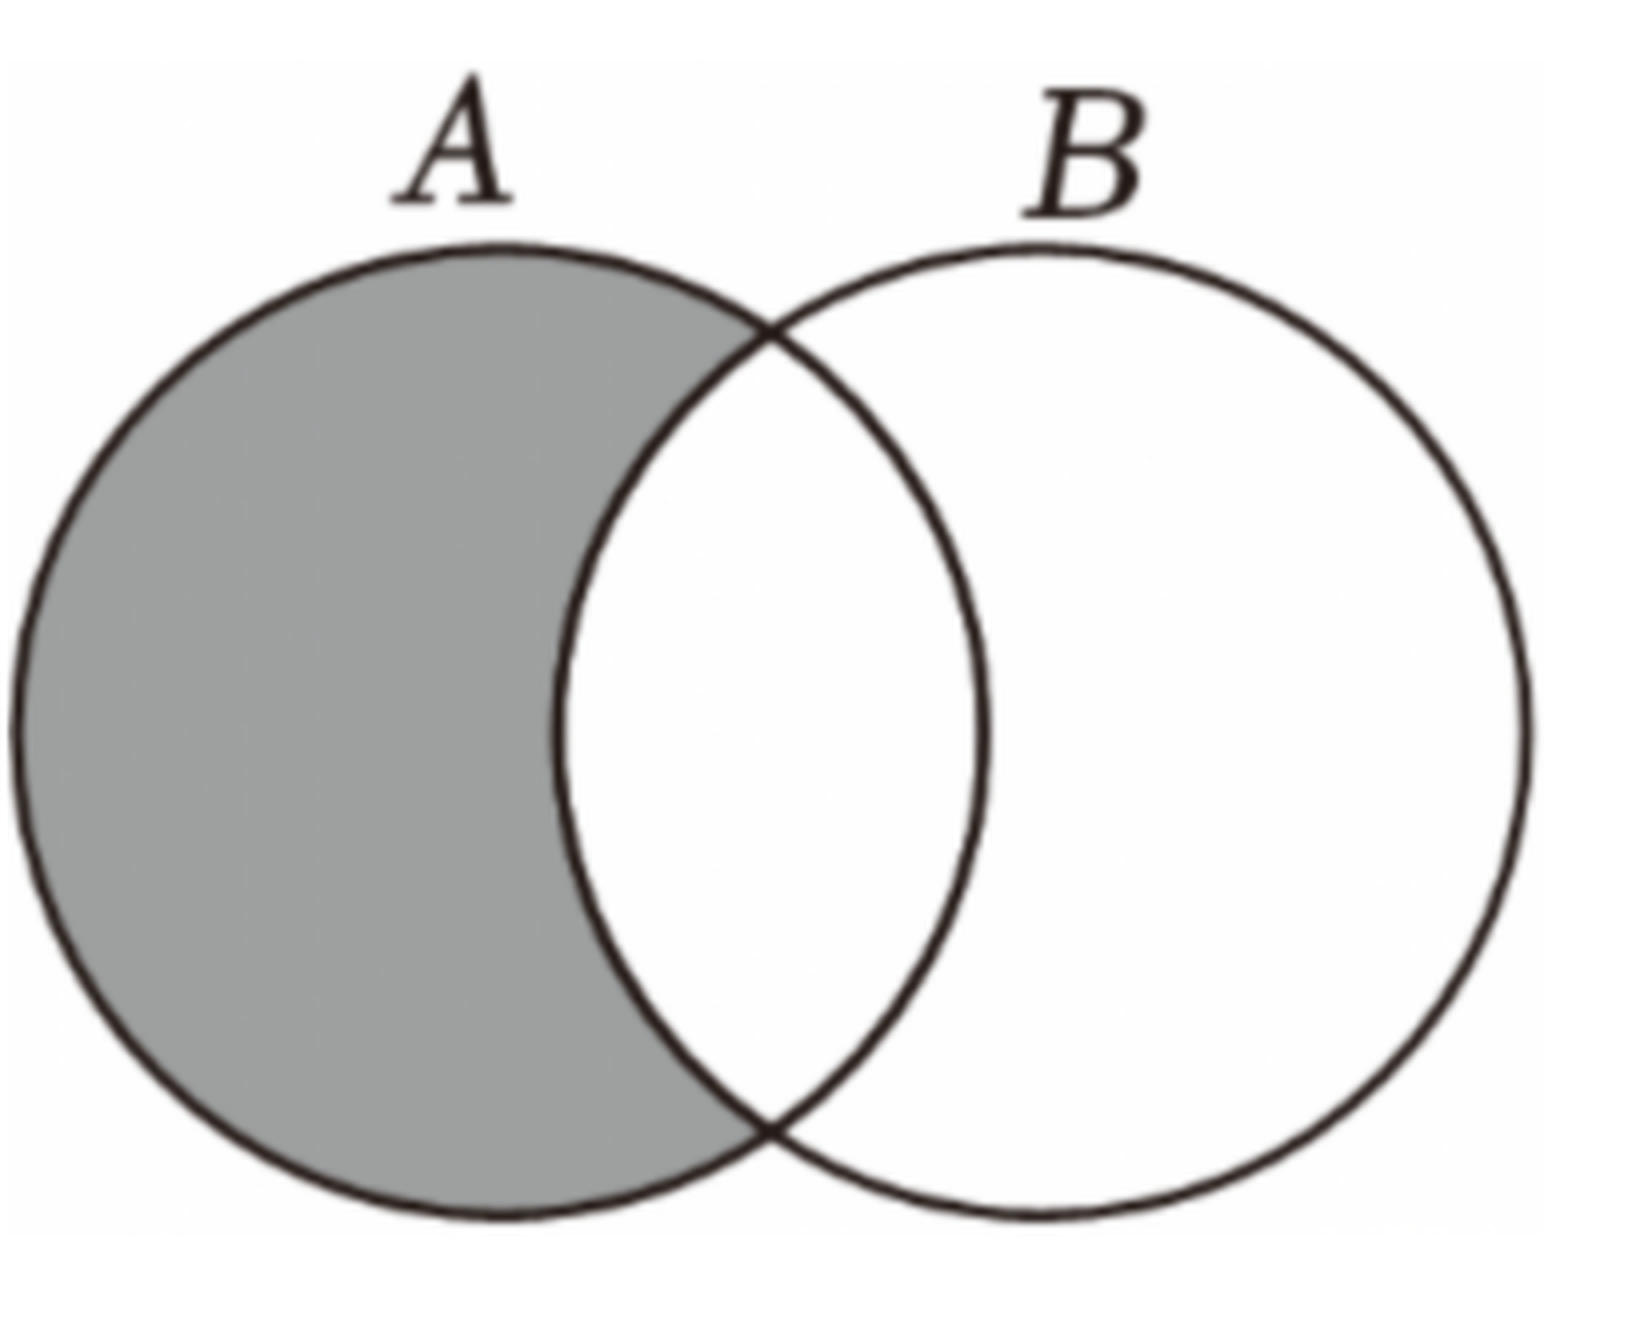
\includegraphics[width=0.30\textwidth]{figures/venn_A_minus_B_h38.png}
\end{center}

\ans{$\{1\}$}

\item 集合 $\{2,3,4,\cdots,2024,2025\}$ 的真子集的个数为 \blankline[4.4em].

\ans{$2^{2024}-1$}

\ifanswer
\solbegin
\step{集合 $\{2,3,4,\cdots,2024,2025\}$ 的真子集的个数为 $2^{2024}-1$.}
\solend

\fi

\item 已知集合 $A$ 中的元素都是正整数，其中最小的是 $1$，最大值是 $100$，除 $1$ 以外，每一个元
素都等于 $A$ 中的两个数（可以相同）的和，则集合 $A$ 中至少含有 \blankline[4.4em] 个元素.

\ans{$9$}

\ifanswer
\solbegin
\step{设 $A$ 中的数从小到大排列为 $1,a_1,a_2,\cdots,a_k,100$，}
\step{则 $a_1=1+1=2$；$3\leqslant a_2\leqslant 4$；$4\leqslant a_3\leqslant 8$；$5\leqslant a_4\leqslant 16$；$6\leqslant a_5\leqslant 32$；$7\leqslant a_6\leqslant 64$；}
\step{于是 $A$ 至少有八个数；}
\step{假设 $A$ 恰好有八个元素，由于 $a_5+a_6\leqslant 96<100$；}
\step{故必须有 $100=a_6+a_6$，$a_6=50$，}
\step{又 $a_4+a_5\leqslant 48$，同理 $a_5=25$，}
\step{但此时 $a_3+a_4\leqslant 24$，$a_5=2a_4$，$a_4=12.5$ 矛盾，}
\step{故 $A$ 不可能恰好有八个元素，因此 $A$ 至少有九个元素.}
\step{其九个数可以为 $1$，$2$，$3$，$6$，$12$，$13$，$25$，$50$，$100$.}
\solend

\fi

\item 已知集合 $\{x_1,x_2,x_3,x_4,x_5,x_6\}=\{1,2,3,4,5,6\}$，将 $x_i$ 与 $x_j$（其中 $i\in\{1,2,3\}$，
$j\in\{4,5,6\}$）的乘积 $x_ix_j$ 放入如图的 $3\times3$ 方格中，则方格中全部数之和的最大值为 \blankline[4.4em].

% 原卷的 $3\times3$ 方格是表格式内容（三行三列的公式），本稿按 高一03 的成例用 tabular 排出。
\begin{center}
\begin{tabular}{|c|c|c|}
\hline
$x_1x_4$ & $x_1x_5$ & $x_1x_6$ \\
\hline
$x_2x_4$ & $x_2x_5$ & $x_2x_6$ \\
\hline
$x_3x_4$ & $x_3x_5$ & $x_3x_6$ \\
\hline
\end{tabular}
\end{center}

\ans{$110$}

\ifanswer
\solbegin
\step{由表格数据得所有数之和为}
\step{$S=x_1x_4+x_1x_5+x_1x_6+x_2x_4+x_2x_5+x_2x_6+x_3x_4+x_3x_5+x_3x_6$，}
\step{所以 $S=(x_1+x_2+x_3)(x_4+x_5+x_6)$，}
\step{因为集合 $\{x_1,x_2,x_3,x_4,x_5,x_6\}=\{1,2,3,4,5,6\}$，}
\step{所以 $x_1+x_2+x_3+x_4+x_5+x_6=1+2+3+4+5+6=21$，}
\step{设 $t=x_1+x_2+x_3$，则 $6\leqslant t\leqslant 15$，$t\in\N^*$，}
\step{$S=t(21-t)=-\left(t-\dfrac{21}{2}\right)^2+\dfrac{441}{4}$，}
\step{当 $t=10$ 或 $t=11$ 时，$S=t(21-t)$ 取最大值，最大值为 $110$，}
\step{此时 $\{x_1,x_2,x_3\}=\{1,4,5\}$，$t=10$，所以可取最大值 $110$.}
\solend

\fi

\item 若 $[x]$ 表示不大于 $x$ 的最大整数，方程 $x^2-8[x]+7=0$ 的解集为 \blankline[4.4em].

\ans{$\{1,\sqrt{33},\sqrt{41},7\}$}

\ifanswer
\solbegin
\step{由题意，$x\geqslant[x]=\dfrac{x^2+7}{8}>0$，得 $x^2-8x+7\leqslant 0$，解得 $1\leqslant x\leqslant 7$，}
\step{$[x]=1$，$x^2=1$，$x=1$；}
\step{$[x]=2$，$x^2=9$，$x=3$ 与 $[x]=2$ 矛盾；}
\step{$[x]=3$，$x^2=17$，$x=\sqrt{17}$，$[x]=4$ 与 $[x]=3$ 矛盾；}
\step{$[x]=4$，$x^2=25$，$x=5$ 与 $[x]=4$ 矛盾；}
\step{$[x]=5$，$x^2=33$，$x=\sqrt{33}$，$[x]=5$；}
\step{$[x]=6$，$x^2=41$，$x=\sqrt{41}$，$[x]=6$；}
\step{$[x]=7$，$x^2=49$，$x=7$；}
\step{综上，方程 $x^2-8[x]+7=0$ 的解集为 $\{1,\sqrt{33},\sqrt{41},7\}$.}
\solend

\fi

\end{enumerate}

\bigsec{二、选择题}

\begin{enumerate}
\setcounter{enumi}{10}

\item 已知集合 $A=\{a,a^2\}$，$B=\{1,3\}$，若 $1\in A$，则 $A\cup B$ 中所有元素之和为\mbox{（\quad）}

\keepwithprev
A. $2$\qquad B. $3$\qquad C. $4$\qquad D. $5$

\ans{$B$}

\ifanswer
\solbegin
\step{因为 $1\in A$，集合 $A=\{a,a^2\}$，所以 $a=1$ 或 $a^2=1$，}
\step{若 $a=1$，则 $a=a^2$，与元素的互异性矛盾；}
\step{若 $a^2=1$，则 $a=1$（舍）或 $a=-1$，故 $A=\{-1,1\}$，$B=\{1,3\}$，}
\step{故 $A\cup B=\{-1,1,3\}$，所以 $A\cup B$ 中所有元素之和为 $-1+1+3=3$. 故选 $B$.}
\solend

\fi

\item 对于实数 $a$、$b$、$c$，下列命题正确的是\mbox{（\quad）}

\keepwithprev
A. 若 $a>b$，则 $ac^2>bc^2$\qquad B. 若 $a>b$，则 $a^2>b^2$

C. 若 $a>b$，则 $a|a|>b|b|$\qquad D. 若 $a>b>c>0$，则 $\dfrac{b}{a-b}<\dfrac{c}{a-c}$

\ans{$C$}

\ifanswer
\solbegin
\step{对于 $A$，若 $a>b$，$c=0$，则 $ac^2=bc^2$，故 $A$ 错误；}
\step{对于 $B$，若 $a>b$，取 $a=-1$，$b=-2$，则 $a^2<b^2$，故 $B$ 错误；}
\step{对于 $C$，若 $a>b>0$ 时，$a|a|-b|b|=a^2-b^2>0$，}
\step{当 $a>0>b$ 时，$a|a|-b|b|=a^2+b^2>0$，}
\step{当 $0>a>b$ 时，$a|a|-b|b|=b^2-a^2=(b-a)(b+a)>0$，}
\step{综上，若 $a>b$，则 $a|a|>b|b|$，故 $C$ 正确；}
\step{对于 $D$，若 $a>b>c>0$，$\dfrac{b}{a-b}-\dfrac{c}{a-c}=\dfrac{ab-bc-ac+bc}{(a-b)(a-c)}=\dfrac{a(b-c)}{(a-b)(a-c)}>0$，}
\step{故 $D$ 错误.}
\step{故选 $C$.}
\solend

\fi

\item 对于正整数集合 $A=\{a_1,a_2,\cdots,a_n\}(n\in\N^*,\ n\geqslant 3)$，如果去掉其中任意一个元素
$a_i(i=1,2,\cdots,n)$ 之后，剩余的所有元素组成的集合都能分为两个交集为空集的集合，且这
两个集合的所有元素之和相等，就称集合 $A$ 为平衡集. 记 $M=a_1+a_2+\cdots+a_n$. 若集合 $A$
是平衡集，并且存在 $a_i$ 为奇数，则集合 $A$ 中元素个数 $n$ 的奇偶性\mbox{（\quad）}

\keepwithprev
A. 与 $M$ 相关，既可以是奇数，又可以是偶数

B. 与 $M$ 无关，既可以是奇数，又可以是偶数

C. 与 $M$ 无关，必为偶数

D. 与 $M$ 无关，必为奇数

\ans{$D$}

\ifanswer
\solbegin
\step{正整数集合 $A=\{a_1,a_2,\cdots,a_n\}(n\in\N^*,\ n\geqslant 3)$，}
\step{因为集合 $A$ 是平衡集，设去掉元素 $a_i(i=1,2,\cdots,n)$，}
\step{由题意得 $A=A_1\cup A_2\cup\{a_i\}$，其中 $A_1\cap A_2=\varnothing$，}
\step{设集合 $A_1$ 和 $A_2$ 中的元素之和均为 $m$，所以 $M=2m+a_i$，其中 $i=1,2,\cdots,n$，}
\step{所以 $M-a_i=2m$，所以 $M-a_i$ 为偶数，其中 $i=1,2,\cdots,n$，}
\step{所以 $a_i(i=1,2,\cdots,n)$ 的奇偶性相同；}
\step{因为存在 $a_i$ 为奇数，所以 $a_i(i=1,2,\cdots,n)$ 均为奇数，}
\step{由 $M-a_i=2m$ 得 $M$ 也为奇数，且 $M=a_1+a_2+\cdots+a_n$，}
\step{所以 $n$ 也为奇数，所以 $n$ 必为奇数. 故选 $D$.}
\solend

\fi

\item 对于集合 $M=\{a\mid a=x^2-y^2,\ x\in\Z,\ y\in\Z\}$，给出如下三个结论：其中正确结论的个数
是\mbox{（\quad）}

\keepwithprev
①如果 $P=\{b\mid b=2n+1,\ n\in\Z\}$，那么 $P\sub M$；

②如果 $c=4n+2$，$n\in\Z$，那么 $c\notin M$；

③如果 $a_1\in M$，$a_2\in M$，那么 $a_1a_2\in M$.

\keepwithprev
A. $1$\qquad B. $2$\qquad C. $3$\qquad D. $0$

\ans{$C$}

\ifanswer
\solbegin
\step{对于①，$b=2n+1$，$n\in\Z$，则恒有 $2n+1=(n+1)^2-n^2$，}
\step{所以 $2n+1\in M$，即 $P=\{b\mid b=2n+1,n\in\Z\}$，则 $P\sub M$，①正确；}
\step{对于②，$c=4n+2$，$n\in\Z$，}
\step{若 $4n+2\in M$，则存在 $x$、$y\in\Z$ 使得 $x^2-y^2=4n+2$，}
\step{所以 $4n+2=(x+y)(x-y)$，又 $x+y$ 和 $x-y$ 同奇或同偶，}
\step{若 $x+y$ 和 $x-y$ 都是奇数，则 $(x+y)(x-y)$ 为奇数，而 $4n+2$ 是偶数；}
\step{若 $x+y$ 和 $x-y$ 都是偶数，则 $(x+y)(x-y)$ 能被 $4$ 整除，而 $4n+2$ 不能被 $4$ 整除，}
\step{所以 $4n+2\notin M$，即 $c\notin M$，②正确；}
\step{对于③，$a_1\in M$，$a_2\in M$，可设 $a_1=x_1^2-y_1^2$，$a_2=x_2^2-y_2^2$，$x_i$、$y_i\in\Z$；}
\step{则 $a_1a_2=(x_1^2-y_1^2)(x_2^2-y_2^2)=(x_1x_2)^2+(y_1y_2)^2-(x_1y_2)^2-(x_2y_1)^2$}
\step{$=(x_1x_2+y_1y_2)^2-(x_1y_2+x_2y_1)^2\in M$，那么 $a_1a_2\in M$，③正确.}
\step{综上，正确的命题是①②③. 故选 $C$.}
\solend

\fi

\end{enumerate}

\bigsec{三、解答题}

\begin{enumerate}
\setcounter{enumi}{14}

\item 已知 $A=\{x\mid a\leqslant x\leqslant -a+3\}$，$B=\{x\mid x<-1\text{ 或 }x>5\}$.

\begin{enumerate}[label=(\arabic*)]

\item 若 $A\cap B=\varnothing$，求 $a$ 的取值范围；

\item 若 $A\cup B=\R$，求 $a$ 的取值范围.

\end{enumerate}

\ans{（1）$[-1,+\infty)$；（2）$(-\infty,-2]$}

\ifanswer
\solbegin
\stepm{(1)}{①当 $A=\varnothing$ 时，$A\cap B=\varnothing$，需满足 $a>-a+3$，解得 $a>\dfrac32$，}
\step{故 $a$ 的取值范围为 $\left(\dfrac32,+\infty\right)$.}
\step{②当 $A\neq\varnothing$ 时，要使 $A\cap B=\varnothing$，需满足
$\begin{cases}a\leqslant\dfrac32\\[4pt] -a+3\leqslant 5\\[4pt] a\geqslant -1\end{cases}$，解得 $-1\leqslant a\leqslant\dfrac32$.}
\step{综上所述，$a$ 的取值范围是 $[-1,+\infty)$.}
\stepm{(2)}{因为 $A\cup B=\R$，$A=\{x\mid a\leqslant x\leqslant -a+3\}$，$B=\{x\mid x<-1\text{ 或 }x>5\}$，}
\step{所以 $\begin{cases}-a+3\geqslant 5\\[4pt] a\leqslant -1\end{cases}$，解得 $a\leqslant -2$，故所求 $a$ 的取值范围为 $(-\infty,-2]$.}
\solend

\fi

\ansspace[6]

\item 已知集合 $A=\{x\mid mx^2+x-2=0\}$，$B=\{x\mid 2x^2-5x-12=0\}$.

\begin{enumerate}[label=(\arabic*)]

\item 若 $A$ 中有且仅有 $1$ 个元素，求实数 $m$ 的值；

\item 已知集合 $C=A\cup B$，若 $C$ 的真子集有且仅有 $3$ 个，求实数 $m$ 的取值范围.

\end{enumerate}

\ans{（1）$m=0$ 或 $m=-\dfrac18$；（2）$\left\{m\mid m\leqslant -\dfrac18\right\}$}

\ifanswer
\solbegin
\stepm{(1)}{若 $m=0$，方程化为 $x-2=0$，此时方程有且仅有一个根 $x=2$；}
\step{若 $m\neq 0$，则 $\Delta=1^2-4\times m\times(-2)=0$，即 $m=-\dfrac18$ 时，}
\step{方程有两个相等的实根，此时集合 $A$ 中有且仅有一个元素，}
\step{所以实数 $m$ 的值为 $m=0$ 或 $m=-\dfrac18$；}
\stepm{(2)}{$B=\{x\mid 2x^2-5x-12=0\}=\left\{-\dfrac32,4\right\}$，}
\step{因为 $C=A\cup B$，若 $C$ 的真子集有且仅有 $3$ 个，则 $C$ 中有两个元素，}
\step{所以 $A\sub B$，由（1）得 $m=0$ 时，$A=\{2\}$，不符合 $A\sub B$，}
\step{当 $m\neq 0$ 时，若 $\Delta=1^2-4\times m\times(-2)<0$，解得 $m<-\dfrac18$，}
\step{此时 $A=\varnothing$，符合 $A\sub B$，}
\step{若 $\Delta=1^2-4\times m\times(-2)=0$，解得 $m=-\dfrac18$，}
\step{此时方程 $mx^2+x-2=0$ 的根为 $x=4$，集合 $A=\{4\}$，符合 $A\sub B$，}
\step{若 $\Delta=1^2-4\times m\times(-2)>0$，由 $A\sub B$，得 $A=\left\{-\dfrac32,4\right\}$，}
\step{此时有 $-\dfrac32+4=-\dfrac1m$ 且 $-\dfrac32\times 4=-\dfrac2m$，无解，}
\step{综上所述，实数 $m$ 的取值范围为 $\left\{m\mid m\leqslant -\dfrac18\right\}$.}
\solend

\fi

\ansspace[6]

\item 设 $A$ 是非空实数集，且 $0\notin A$. 若对于任意的 $x$、$y\in A$，都有 $xy\in A$，则称集合 $A$ 具
有性质 $P_1$；若对于任意的 $x$、$y\in A$，都有 $\dfrac xy\in A$，则称集合 $A$ 具有性质 $P_2$.

\begin{enumerate}[label=(\arabic*)]

\item 写出一个恰含有两个元素且具有性质 $P_1$ 的集合 $A$，并说明理由；

\item 证明：“非空实数集 $A$ 具有性质 $P_1$”是“非空实数集 $A$ 具有性质 $P_2$”的必要非充分条
件.

\end{enumerate}

\ans{（1）$A=\{-1,1\}$，理由见解析；（2）见解析}

\ifanswer
\solbegin
% 注：原卷本题 (1) 的解析里“证明”一词重复出现两次（一次接在分号后、一次另起一行），
%     本稿照原卷重复录入，未去重。
\stepm{(1)}{$A=\{-1,1\}$，证明：恰含有两个元素且具有性质 $P_1$ 的集合 $A=\{-1,1\}$；}
\step{证明：$1\times 1=1\in A$，$1\times(-1)=-1\in A$，$-1\times 1=-1\in A$，$-1\times(-1)=1\in A$；}
\stepm{(2)}{若集合 $A$ 具有性质 $P_2$，不妨设 $a\in A$，}
\step{由非空数集 $A$ 具有性质 $P_2$，有 $\dfrac aa=1\in A$.}
\step{①$A=\{1\}$，易得此时集合 $A$ 具有性质 $P_1$.}
\step{②数集 $A$ 只含有两个元素，不妨设 $A=\{1,a_1\}$，}
\step{由 $\dfrac{1}{a_1}=a_1$，且 $a_1\neq 1$，解得 $a_1=-1$，此时集合 $A$ 具有性质 $P_1$.}
\step{③实数集 $A$ 含有两个以上的元素，不妨设不为 $1$ 的元素 $a_1$、$a_2\in A$，}
\step{则有 $\dfrac{1}{a_1}\in A$，由于集合 $A$ 具有性质 $P_2$，}
\step{所以有 $a_2\div\dfrac{1}{a_1}=a_1a_2\in A$，这说明集合 $A$ 具有性质 $P_1$.}
\step{综上，若非空实数集 $A$ 具有性质 $P_2$，则集合 $A$ 具有性质 $P_1$，}
\step{所以“非空实数集 $A$ 具有性质 $P_1$”是“非空实数集 $A$ 具有性质 $P_2$”的}
\step{必要条件.}
\step{取正偶数集 $A=\{x\mid x=2n,\ n\in\N^*\}$，}
\step{对任意的 $2m$、$2n\in A$，$m$、$n\in\N^*$，}
\step{有 $2m\times 2n=4mn\in A$，故 $A$ 具有性质 $P_1$，}
\step{取 $x=2$，$y=4$，则 $\dfrac xy=\dfrac12\notin A$，故 $A$ 不具有性质 $P_2$，}
\step{所以“非空实数集 $A$ 具有性质 $P_1$”不是“非空实数集 $A$ 具有性质 $P_2$”的}
\step{充分条件.}
\step{综上，“非空实数集 $A$ 具有性质 $P_1$”是“非空实数集 $A$ 具有性质 $P_2$”的}
\step{必要非充分条件.}
\solend

\fi

\ansspace[8]

\item 已知命题 $p$：关于 $x$ 的方程 $x^2+mx+1=0$ 有两个不同的正根；命题 $q$：关于 $x$ 的方程
$4x^2+4(m-2)x=-1$ 有实根.

\begin{enumerate}[label=(\arabic*)]

\item 若命题 $q$ 为假命题，求整数 $m$ 的解集；

\item 若命题 $p$ 为真命题，且关于 $x$ 的方程 $x^2+mx+1=0$ 的两个实数根 $x_1$、$x_2$ 满足
$3x_1+2x_2=5$，求实数 $m$ 的取值集合；

\item 若命题 $p$ 和命题 $q$ 有且仅有一个成立，求实数 $m$ 的取值范围.

\end{enumerate}

\ans{（1）$\{2\}$；（2）$\left\{-\dfrac{13}{6}\right\}$；（3）$[-2,1]\cup[3,+\infty)$}

\ifanswer
\solbegin
\stepm{(1)}{命题 $q$：关于 $x$ 的方程 $4x^2+4(m-2)x=-1$ 有实根为假命题，}
\step{即 $4x^2+4(m-2)x+1=0$ 无实根，}
\step{则 $\Delta=16(m-2)^2-16<0$，则 $1<m<3$，则整数 $m$ 的解集为 $\{2\}$；}
\stepm{(2)}{若命题 $p$ 为真命题，且关于 $x$ 的方程 $x^2+mx+1=0$ 的两个实数根 $x_1$、$x_2$，}
\step{满足 $3x_1+2x_2=5$，则方程 $x^2+mx+1=0$ 有两个不同的正根，}
\step{则 $\begin{cases}\Delta=m^2-4>0\\[4pt] x_1+x_2=-m>0\end{cases}$，则 $m<-2$，}
\step{又 $\begin{cases}x_1+x_2=-m\\[4pt] x_1x_2=1\\[4pt] 3x_1+2x_2=5\end{cases}$，
则 $\begin{cases}x_1=5+2m\\[4pt] x_2=-3m-5\end{cases}$，则 $(5+2m)(-3m-5)=1$，}
\step{得 $m=-2$ 或 $m=-\dfrac{13}{6}$，又因为 $m<-2$，所以 $m=-\dfrac{13}{6}$，}
\step{所以实数 $m$ 的取值集合为 $\left\{-\dfrac{13}{6}\right\}$；}
\stepm{(3)}{由（2）得当 $p$ 为真时，则有 $m<-2$，}
\step{当 $q$ 为真时，$\Delta=16(m-2)^2-16\geqslant 0$，解得 $m\leqslant 1$ 或 $m\geqslant 3$，}
\step{又因为命题 $p$ 和命题 $q$ 只有一个为真，所以
$\begin{cases}m<-2\\[4pt] 1<m<3\end{cases}$ 或 $\begin{cases}m\geqslant -2\\[4pt] m\leqslant 1\text{ 或 }m\geqslant 3\end{cases}$，}
\step{解得 $-2\leqslant m\leqslant 1$ 或 $m\geqslant 3$，所以实数 $m$ 的取值范围为 $[-2,1]\cup[3,+\infty)$.}
\solend

\fi

\ansspace[8]

% 注：原卷此处作“设 $n\in\N^*$，集合含有 $3n$ 个元素”，**漏了符号 $U$**（应作“集合 $U$
%     含有 $3n$ 个元素”）——$U$ 直到本句末尾“则称 $U$ 为三分集合”才出现、此前无定义。
%     本稿照录未补，见文件头“原卷笔误/存疑”⑦。
\item 设 $n\in\N^*$，集合含有 $3n$ 个元素，若存在三个 $n$ 元集合 $A$、$B$、$C$ 满足如下两个条件，
则称 $U$ 为三分集合.

①$U=A\cup B\cup C$；

②$A$、$B$、$C$ 元素可分别排列为有序数组 $(a_1,a_2,\cdots,a_n)$，$(b_1,b_2,\cdots,b_n)$ 及
$(c_1,c_2,\cdots,c_n)$，使得对 $\forall i=1,2,\cdots,n$，均有 $a_i+b_i=c_i$.

特别地，当 $U=\{1,2,3,4,\cdots,3n-2,3n-1,3n\}$ 为三分集合时，称 $n$ 为完美三分数.

如：因为 $U=\{1,2,3\}$ 为三分集合，所以 $n=1$ 为最小完美三分数.

\begin{enumerate}[label=(\arabic*)]

\item 请判断下列两个集合是否为三分集合（直接写出结论）：

$U_1=\{1,2,3,4,5,6\}$，$U_2=\{1,3,5,7,8,9,10,11,12\}$；

\item 求出大于 $1$ 的最小完美三分数；

\item 请判断是否存在无穷多个完美三分数？若存在，请说明理由；若不存在，则求出最大的
完美三分数.

\end{enumerate}

\ans{（1）$U_1$ 不是三分集合，$U_2$ 是三分集合；（2）$4$；（3）存在，理由见解析}

\ifanswer
\solbegin
\stepm{(1)}{(i)$U_1=\{1,2,3,4,5,6\}$ 不是三分集合，下面用反证法证明：}
\step{证明：假设 $U=\{1,2,3,4,5,6\}$ 是三分集合，}
\step{设 $A=\{a_1,a_2\}$，$B=\{b_1,b_2\}$，$C=\{c_1,c_2\}$，不妨设 $c_1<c_2$，}
\step{因为 $a_1+b_1=c_1$，$a_2+b_2=c_2$，}
\step{所以 $a_1+b_1+a_2+b_2+c_1+c_2=2(c_1+c_2)=1+2+3+4+5+6=21$，}
% 注：原卷此步印“所以 $c_1+c_2=2$”，与上一行的 $2(c_1+c_2)=21$ **不自洽**
%     （应作 $\dfrac{21}2$）；同题 $n=3$ 处的同型推理原卷写的是 $\dfrac{45}2$，故此处是原卷笔误。
%     本稿照录未改，见文件头“原卷笔误/存疑”⑧。
\step{所以 $c_1+c_2=2$，这与 $c_1,c_2\in\N^*$ 矛盾，故假设错误，}
\step{故 $U_1=\{1,2,3,4,5,6\}$ 不是三分集合；}
\step{(ii)$U_2=\{1,3,5,7,8,9,10,11,12\}$ 是三分集合，理由如下：}
\step{令 $A=\{1,3,5\}$，$B=\{9,8,7\}$，$C=\{10,11,12\}$，}
\step{则 $A\cup B\cup C=U=\{1,3,5,7,8,9,10,11,12\}$，满足条件①；}
\step{又 $1+9=10$；$3+8=11$；$5+7=12$，所以满足条件②，}
\step{所以 $U_2=\{1,3,5,7,8,9,10,11,12\}$ 是三分集合；}
\stepm{(2)}{由（1）得，当 $n=2$ 时，$U=\{1,2,3,4,5,6\}$ 不是三分集合；}
\step{当 $n=3$ 时，$U=\{1,2,3,4,5,6,7,8,9\}$，}
\step{假设 $U=\{1,2,3,4,5,6,7,8,9\}$ 是三分集合，}
\step{同理由 $a_1+b_1+a_2+b_2+a_3+b_3+c_1+c_2+c_3$}
\step{$=2(c_1+c_2+c_3)=1+2+\cdots+9=45$，$c_1+c_2+c_3=\dfrac{45}{2}$，}
\step{可推出与 $c_1$、$c_2$、$c_3\in\N^*$ 矛盾，故假设也错误，}
\step{所以 $U=\{1,2,3,4,5,6,7,8,9\}$ 不是三分集合；}
\step{当 $n=4$ 时，$U=\{1,2,3,\cdots,12\}$，}
\step{存在三个 $4$ 元集合 $A=\{1,2,4,3\}$，$B=\{5,8,7,9\}$，$C=\{6,10,11,12\}$，}
\step{满足 $U=\{1,2,3,\cdots,12\}$ 为三分集合的两个条件，}
\step{故大于 $1$ 的最小完美三分数为 $4$；}
\stepm{(3)}{存在无穷多个完美三分数，理由如下：}
\step{由题意得，$n=1$ 为最小完美三分数，}
\step{当 $n=5$ 时，$U=\{1,2,3,\cdots,15\}$，}
\step{存在三个 $5$ 元集合 $A=\{1,3,5,7,2\}$，$B=\{11,10,9,8,4\}$，$C=\{12,13,14,15,6\}$，}
\step{满足三分集合的条件，故 $5$ 为完美三分数；}
\step{当 $n=21$ 时，$U=\{1,2,3,\cdots,63\}$，}
\step{存在如下三个 $21$ 元的集合满足三分集合的条件：}
\step{$A=\{1,3,5,7,\cdots,29,31,2,6,10,14,4\}$，}
\step{$B=\{47,46,45,44,\cdots,33,32,22,20,18,16,8\}$，}
\step{$C=\{48,49,50,51,\cdots,62,63,24,26,28,30,12\}$，}
\step{故 $21$ 为完美三分数.}
\step{首先证明：若 $n=k$，$k\in\N^*$ 为三分完美数，}
\step{则 $n=4k+1$，$k\in\N^*$ 也为三分完美数，}
% 注：下一行原卷印作“$U_{k+1}=U_{k+1}=\{2,3,\cdots,12k+3\}$”——等号两边记号相同，
%     依上下文疑当作 $U'_{k+1}=U_{4k+1}$，且此处集合自 2 起（前文 $U_{4k+1}$ 自 1 起）；
%     本稿照录原卷，未代为改写。
\step{证明：记 $U_k=\{1,2,3,\cdots,3k\}$，$U_{4k+1}=\{1,2,3,\cdots,12k+3\}$，}
\step{若 $n=k$，$k\in\N^*$ 为三分完美数，则 $U_k$ 为三分集合，}
\step{即存在三个 $k$ 元集合 $A$、$B$、$C$ 满足如下两个条件，}
\step{①$U_k=A\cup B\cup C$；}
\step{②$A$、$B$、$C$ 元素可分别排列为有序数组 $(a_1,a_2,\cdots,a_k)$，}
\step{$(b_1,b_2,\cdots,b_k)$ 及 $(c_1,c_2,\cdots,c_k)$，}
\step{使得对 $\forall i=1,2,3,\cdots,k$，均有 $a_i+b_i=c_i$，}
\step{则可得到对 $\forall i=1,2,3,\cdots,k$，$2a_i+2b_i=2c_i$，}
\step{故集合 $\{2,4,6,\cdots,6k\}$ 也满足三分集合的两个条件，其也为三分集合，}
\step{下面记集合 $\{2,4,6,\cdots,6k\}=2U_k$，}
\step{对 $n=4k+1$，集合 $U_{k+1}=U_{k+1}=\{2,3,\cdots,12k+3\}=(2U_k)\cup\complement_{U_{4k+1}}(2U_k)$，}
\step{构造集合 $A'=\{1,3,5,7,\cdots,6k+1\}$，共有 $3k+1$ 个奇数；}
% 注：下一行原卷印作“$B'=\{6k+3k+2,6k+3k+1,6k+3k,6k+3k-1,\cdots,6k+2\}$”，
%     按与后文 $C'$ 相接，前四项当写作 $9k+2$、$9k+1$、$9k$、$9k-1$；本稿照录原卷。
\step{集合 $B'=\{6k+3k+2,6k+3k+1,6k+3k,6k+3k-1,\cdots,6k+2\}$，}
\step{共有 $3k+1$ 个逐个减小的连续正整数；}
\step{集合 $C'=\{9k+3,9k+4,9k+5,9k+6,\cdots,12k+3\}$，}
\step{共有 $3k+1$ 个逐个增大的连续正整数；}
\step{得这三个 $3k+1$ 元集合 $A'$、$B'$、$C'$ 满足如下两个条件，}
\step{①集合 $A'\cup B'\cup C'=\complement_{U_{4k+1}}(2U_k)$；}
\step{②$A'$、$B'$、$C'$ 元素可分别排列为有序数组 $(a_1,a_2,\cdots,a_{3k+1})$，}
\step{$(b_1,b_2,\cdots,b_{3k+1})$ 及 $(c_1,c_2,\cdots,c_{3k+1})$，}
\step{使得对 $\forall i=1,2,3,\cdots,3k+1$，均有 $a_i+b_i=c_i$；}
\step{故 $\complement_{U_{4k+1}}(2U_k)$ 为三分集合，而已知 $U_k$ 为三分集合，}
\step{将其对应与 $A'$、$B'$、$C'$ 合并，}
% 注：原卷此处印“令 $A''=A\cup A'$”（$B''$、$C''$ 同）。按同段上文“记集合
%     $\{2,4,6,\cdots,6k\}=2U_k$”，此处疑当作 $A''=2A\cup A'$——否则
%     $A''\cup B''\cup C''=U_k\cup\complement_{U_{4k+1}}(2U_k)\neq U_{4k+1}$，与本段结论冲突。
%     本稿照录未改，见文件头“原卷笔误/存疑”⑨。
\step{令 $A''=A\cup A'$，$B''=B\cup B'$，$C''=C\cup C'$，}
\step{则这三个 $4k+1$ 元集合 $A''$、$B''$、$C''$，}
\step{满足 $A''\cup B''\cup C''=U_{4k+1}$，且满足条件②，}
\step{故 $U_{4k+1}=\{1,2,3,\cdots,12k+3\}$ 为三分集合，}
\step{因此可得，若 $n=k$ 为三分完美数，则 $n=4k+1$ 也为三分完美数，}
\step{由 $1$，$5$，$21$ 为完美三分数，结合所证结论得，存在无穷多个完美三分数.}
\solend

\fi

\ansspace*[12]

\end{enumerate}

\end{document}
"
%
% 原始材料是微信公众号图文（公众号“魔都数学加油站”连载“27学年高一 38”，署名“破晓”，
% 2026-09-26 21:29 发布，原文标题“27学年高一38——2026-2027年上海市大同中学高一上周末作业3”，
% 原文链接 https://mp.weixin.qq.com/s/O_O60vCIiGi2xponAo4irw ），正文为 12 张 PNG 页。
% **同一篇里各页分辨率不一致**（2560×3620 与 4762×6735 两档混排：第 1、10、11、12 页为
% 2560×3620，第 2—9 页为 4762×6735）。原文本身就是一份**讲评版**——有的题下方只印
% 【答案】行，有的只印【解析】。试题文字、答案与解析均照原卷录入，未改内容。卷面的粉色
% 斜水印“魔都数学加油站”属水印，未录入。
%
% 本卷共 **17 题**：填空题 8 题（第 3—10 题）、选择题 4 题（第 11—14 题）、解答题 5 题
% （第 15—19 题）；插图 1 张（第 6 题 Venn 图）。三版页数：试卷版 4 页 / 答案版 11 页 /
% 紧凑版 3 页，`Overfull`／`Underfull`／`Missing character` 告警均为 0。
%
% 卷首标题：原卷印作“2026-2027 年大同中学高一上周末作业 3”（公众号原文标题里的“上海市”
% 三字卷面标题行没有，本稿照卷面），年份区间按全稿惯例排 en dash，前缀照原卷保留“年”。
%
% 与原卷的排版差异（均已在 README“说明”中交代）：
%   ① 原文自**第 3 题**起（第 1、2 题未在该文中发布），故本稿题号亦自 3 起，填空题以
%      \setcounter{enumi}{2} 起编；选择、解答两节各按上一节末号另设 \setcounter
%      （选择题 \setcounter{enumi}{10}、解答题 \setcounter{enumi}{14}）；
%   ② 原卷本就印有“一、填空题”“二、选择题”“三、解答题”三节标题，本稿照原卷分节，
%      只把标题改排成全稿统一的“大节标题”样式；
%   ③ 原卷是“讲评版”：第 3、6 题只印【答案】行，第 4、5、7、8、9、10 题与第 11—19 题印
%      【解析】；本稿统一改为试卷版隐去、答案版以 \ans{}／\ifanswer 块给出，两版彻底分离。
%      其中第 4、5、7、8、9、10 题与第 11—14 题的答案，原卷写在【解析】末句，本稿另提为
%      \ans{}；第 15—19 题原卷只有【解析】、无独立答案行，本稿亦补了摘要式 \ans{}。
%      **故本卷 17 题每题都有 \ans**——比“只印【解析】的填空、解答题不另提 \ans”的
%      高一31／高一34 更彻底，与 高一21 第 11 题（填空，答案在【解析】末句，本稿另提）同类；
%      （本仓对“另提 \ans{}”的做法各卷不一，见 README 对应专记的核对面。）
%   ④ 数集记号原卷两套并用：第 3、5 题的实数集作粗体 $\mathbf{R}$，第 8、14、17、18 题等的
%      整数集、自然数集作斜体 $Z$、$N$，本稿按全稿惯例统一写作 $\R$、$\Z$、$\N$；
%   ⑤ 原卷填空的横线宽度不一（约 1.8—3.6 字宽），本稿按全稿惯例统一排 \blankline[4.4em]；
%   ⑥ 中文括注原卷用半角“(  )”，本稿按全稿惯例排全角；选择题的作答括注统一排
%      \mbox{（\quad）}（第 14 题的作答括注原卷印在 ①②③ 三个命题**之前**，本稿照原卷次序）；
%      数学式内部的括注（如第 4 题的 $p\%(0<p<100)$、第 13 题的 $a_i(i=1,2,\cdots,n)$）照原样
%      留在行内公式里，未改全角；
%   ⑦ 原卷并列的字母（“x,y”“a,b,c”）不加标点或作半角逗号，本稿按全稿惯例改排顿号；
%   ⑧ 第 6 题的 Venn 图取原卷截图、4× LANCZOS 放大（figures/venn_A_minus_B_h38.png，
%      见该处 \includegraphics 前的注释）；第 9 题的 $3\times3$ 方格属**表格式**内容，
%      本稿按 高一03 的成例用 tabular 排出，未截图；
%   ⑨ 原卷未印副标题，本稿按**本卷实际内容**补出副标题“集合与常用逻辑用语”（依据见下条）；
%   ⑩ 原卷【解析】**一个印刷行照录为一条 `\step`**（原卷的折行也照录为独立一条，如第 17 题
%      末三处“…的”／“必要条件.”这类跨行句、第 9 题“由表格数据得所有数之和为”／
%      “$S=\cdots$，”），使答案版的排布与原卷讲评版逐行对应；全卷 15 处【解析】合计
%      **191 条 `\step` ＝ 原卷 191 行**（逐处：5、5、1、9、9、9、4、9、9、12、6、14、21、13、65）。
%
% 副标题（\examtitlest 第二个参数）：本卷卷面未印副标题，由本稿补出，取值按 2026-09-26 起的
%   新口径“只用本卷实际内容的模块名”定为“集合与常用逻辑用语”。依据：全卷 17 题
%   （第 3—19 题）中，第 3、5、6、7、8、9、10、11、13、14、15、16、17、18、19 题共 15 题
%   是集合的运算与关系、子集计数、集合新定义（性质 $P_1$／$P_2$、平衡集、三分集合），以及
%   命题与逻辑（第 3 题即用反证法证明“$x+y>2\Rightarrow x>1$ 或 $y>1$”这一命题）；不等式只
%   出现在第 4 题（降价提价的应用比较）、第 12 题（不等式命题真假）与第 10 题解析里解一元
%   二次不等式，合计不足全卷的三分之一，故不并标“不等式”。
%
% 原卷笔误/存疑（均照抄原卷、未改，见源码中该处上方注释）：
%   ① 第 19 题 (3) 的证明里印作“集合 $U_{k+1}=U_{k+1}=\{2,3,\cdots,12k+3\}$”——等号两边
%      记号相同（依上下文疑当作 $U'_{k+1}=U_{4k+1}$），且此处集合自 $2$ 起，而前文
%      $U_{4k+1}=\{1,2,3,\cdots,12k+3\}$ 自 $1$ 起；本稿照录；
%   ② 第 19 题 (3) 的证明里印作
%      “$B'=\{6k+3k+2,6k+3k+1,6k+3k,6k+3k-1,\cdots,6k+2\}$”——按与后文
%      $C'=\{9k+3,9k+4,9k+5,9k+6,\cdots,12k+3\}$ 相接，前四项当写作 $9k+2$、$9k+1$、
%      $9k$、$9k-1$（即 $6k+3k+2$ 等），原卷即作“$6k+3k+\cdots$”形式，本稿照录；
%   ③ 第 19 题的术语前后不一：题干与 (1)(2)(3) 用“完美三分数”，而 (3) 的证明里五次写作
%      “三分完美数”（词序不同）；本稿五处都照录；
%   ④ 第 14 题题干作“给出如下三个结论：其中正确结论的个数是（\quad）”，此处冒号疑当作
%      逗号，本稿照录；
%   ⑤ 第 17 题题干作“非空实数集”，其解析有一处写作“非空数集”；本稿照录；
%   ⑥ 第 17 题 (1) 的【解析】原卷连写“…集合 $A=\{-1,1\}$；证明：…；证明：…”，“证明”
%      一词重复出现两次（第一次在分行处、第二次另起一行），本稿照原卷重复录入，未去重。
%   ⑦ 第 19 题**题干漏字**：原卷作“19.设 $n\in\N^*$，集合含有 $3n$ 个元素…则称 $U$ 为
%      三分集合”——首句漏了符号 $U$（应作“集合 $U$ 含有 $3n$ 个元素”），$U$ 直到结论句
%      才出现、此前无定义；本稿照录未补（见该处上方注释）。
%   ⑧ 第 19(1)(i) 的【解析】**自相矛盾**：上一行印“$a_1+b_1+a_2+b_2+c_1+c_2=2(c_1+c_2)
%      =1+2+3+4+5+6=21$”，下一行却印“所以 $c_1+c_2=2$”（由 $2(c_1+c_2)=21$ 应得
%      $c_1+c_2=\dfrac{21}2$，非整数、才与 $c_1,c_2\in\N^*$ 矛盾）；同题 $n=3$ 处的同型
%      推理原卷就写对了（$\dfrac{45}2$），故此处是原卷笔误；本稿照录未改（见该处上方注释）。
%   ⑨ 第 19(3) 的【解析】印“令 $A''=A\cup A'$，$B''=B\cup B'$，$C''=C\cup C'$”——按同段
%      上文“记集合 $\{2,4,6,\cdots,6k\}=2U_k$”，$A''$ 等疑当作 $2A\cup A'$（$B''$、$C''$ 同），
%      否则 $A''\cup B''\cup C''=U_k\cup\complement_{U_{4k+1}}(2U_k)\neq U_{4k+1}$；本稿照录未改
%      （见该处上方注释）。

\documentclass[a4paper,11pt]{article}
\usepackage{common}

\begin{document}

\examtitlest[3]{2026--2027 年大同中学高一上周末作业 3}{集合与常用逻辑用语}

\bigsec{一、填空题}

\begin{enumerate}
% 原卷填空题自第 3 题起（第 1、2 题未在该文中发布），须与选择、解答两节的 \setcounter 对齐
\setcounter{enumi}{2}

\item 设 $x$、$y\in\R$，若 $x+y>2$，则 $x>1$ 或 $y>1$ 是真命题. 这个命题可以用反证法去证明，
可以假设：\blankline[4.4em].

\ans{$x\leqslant 1$ 且 $y\leqslant 1$}

\item 已知某商品的原价为 $a$ 元，由于市场原因，先降价 $p\%(0<p<100)$ 出售，一段时间后，
再提价 $p\%$ 出售，则该商品提价后的售价 \blankline[4.4em] 该商品的原价（填“高于”“低于”或“等于”）.

\ans{低于}

\ifanswer
\solbegin
\step{由题意得第一次降价后的售价为 $a(1-p\%)$ 元，}
\step{第二次提价后的售价为 $a(1-p\%)(1+p\%)$ 元，}
\step{因为 $0<p<100$，所以 $0<p\%<1$，}
\step{因为 $a(1-p\%)(1+p\%)=a[1-(p\%)^2]<a$，}
\step{即该商品提价后的售价低于该商品的原价.}
\solend

\fi

\item 若集合 $A=\{x\mid ax^2+ax+1=0,\ a\in\R,\ x\in\R\}$ 的子集只有两个，则实数 $a=$ \blankline[4.4em].

\ans{$4$}

\ifanswer
\solbegin
\step{集合 $A=\{x\mid ax^2+ax+1=0\}$ 的子集只有两个，}
\step{所以 $A$ 有且只有一个元素，}
\step{①若 $a=0$，则 $A=\varnothing$ 不成立；}
\step{②若 $a\neq 0$，则 $\Delta=a^2-4a=0$，解得 $a=4$（$0$ 舍）.}
\step{故 $a=4$.}
\solend

\fi

\item 如图，已知集合 $A=\{1,2,3,4,5\}$，集合 $B=\{2,3,4,5,9\}$，则图中阴影部分所表示的
集合为 \blankline[4.4em].

% 图取原卷截图（01.png，2560×3620）右栏，4× LANCZOS 放大；为避免与 高一11 的
% figures/venn_A_minus_B.png 同名，按 高一32 的成例加 _h38 后缀。
\begin{center}
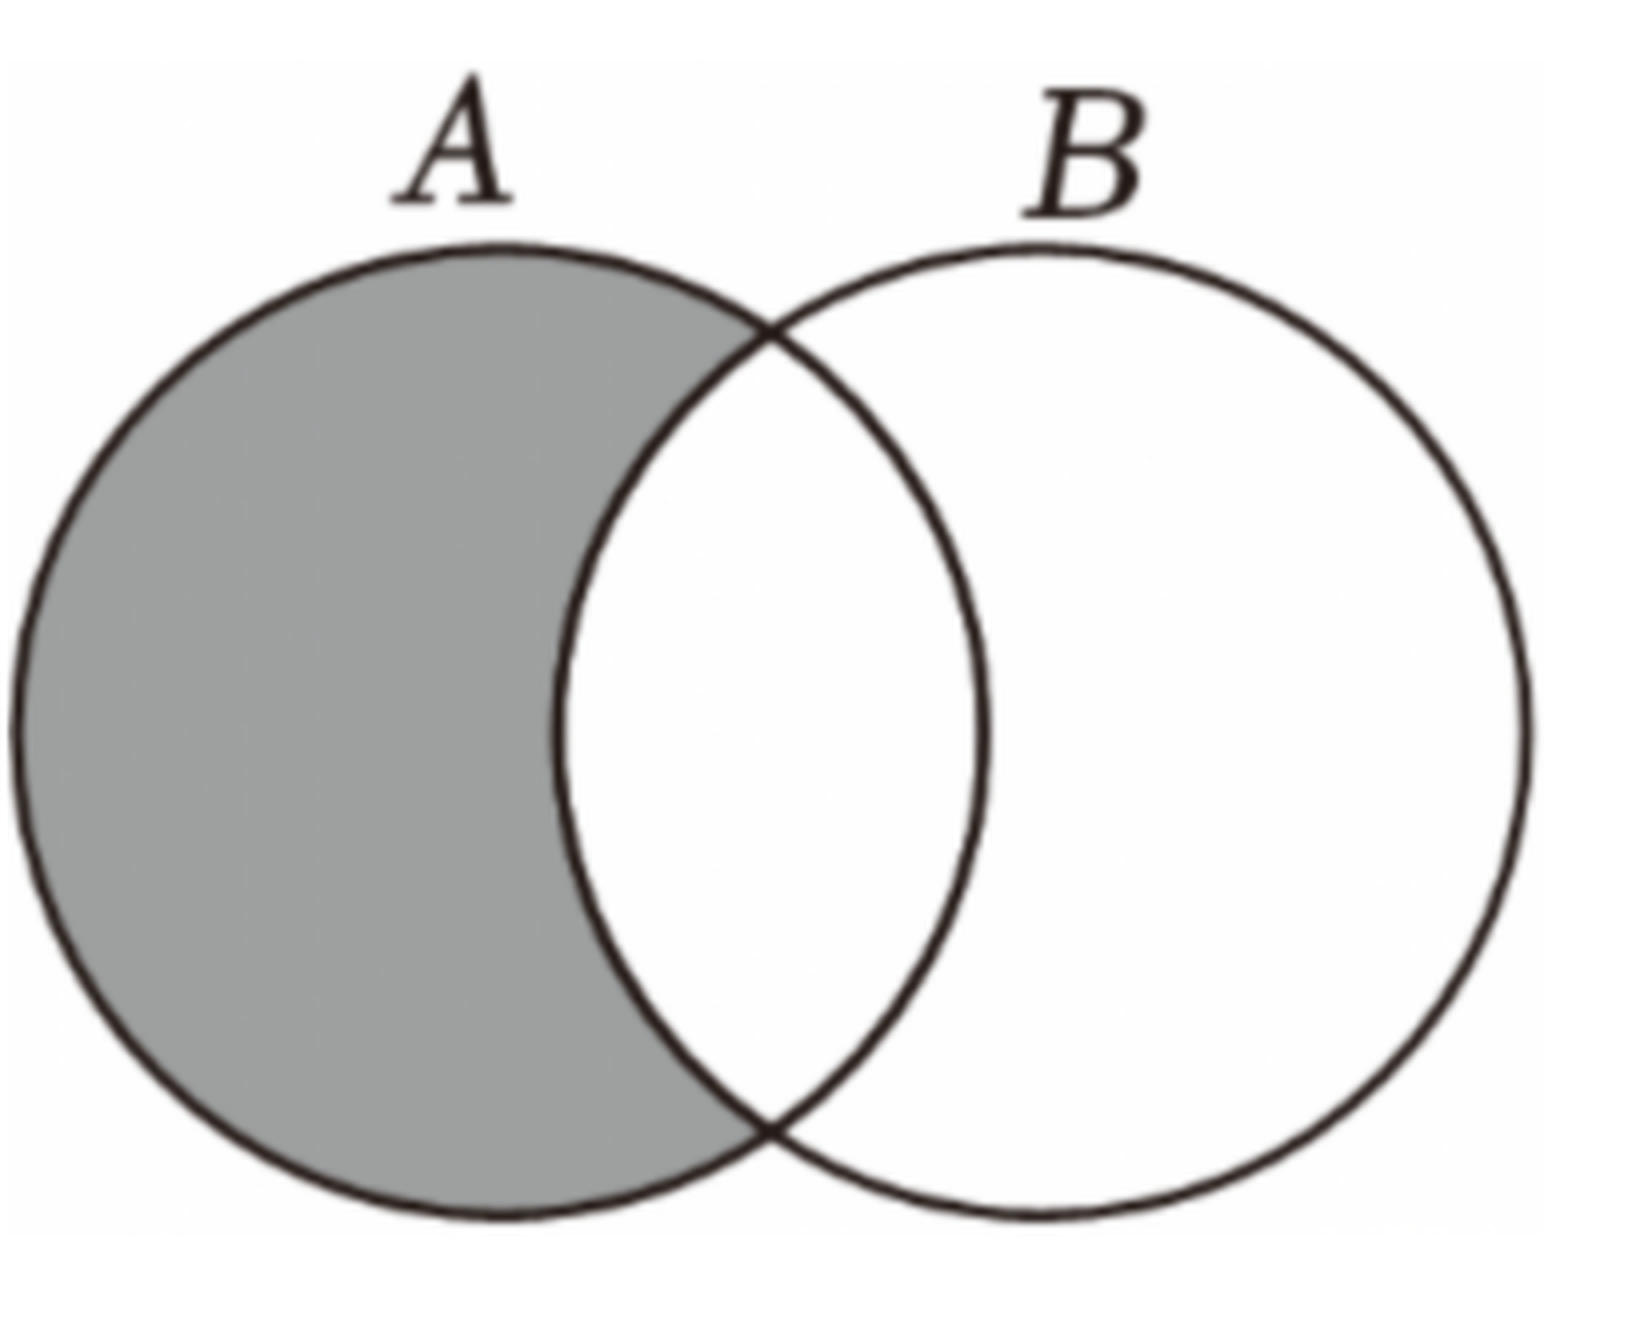
\includegraphics[width=0.30\textwidth]{figures/venn_A_minus_B_h38.png}
\end{center}

\ans{$\{1\}$}

\item 集合 $\{2,3,4,\cdots,2024,2025\}$ 的真子集的个数为 \blankline[4.4em].

\ans{$2^{2024}-1$}

\ifanswer
\solbegin
\step{集合 $\{2,3,4,\cdots,2024,2025\}$ 的真子集的个数为 $2^{2024}-1$.}
\solend

\fi

\item 已知集合 $A$ 中的元素都是正整数，其中最小的是 $1$，最大值是 $100$，除 $1$ 以外，每一个元
素都等于 $A$ 中的两个数（可以相同）的和，则集合 $A$ 中至少含有 \blankline[4.4em] 个元素.

\ans{$9$}

\ifanswer
\solbegin
\step{设 $A$ 中的数从小到大排列为 $1,a_1,a_2,\cdots,a_k,100$，}
\step{则 $a_1=1+1=2$；$3\leqslant a_2\leqslant 4$；$4\leqslant a_3\leqslant 8$；$5\leqslant a_4\leqslant 16$；$6\leqslant a_5\leqslant 32$；$7\leqslant a_6\leqslant 64$；}
\step{于是 $A$ 至少有八个数；}
\step{假设 $A$ 恰好有八个元素，由于 $a_5+a_6\leqslant 96<100$；}
\step{故必须有 $100=a_6+a_6$，$a_6=50$，}
\step{又 $a_4+a_5\leqslant 48$，同理 $a_5=25$，}
\step{但此时 $a_3+a_4\leqslant 24$，$a_5=2a_4$，$a_4=12.5$ 矛盾，}
\step{故 $A$ 不可能恰好有八个元素，因此 $A$ 至少有九个元素.}
\step{其九个数可以为 $1$，$2$，$3$，$6$，$12$，$13$，$25$，$50$，$100$.}
\solend

\fi

\item 已知集合 $\{x_1,x_2,x_3,x_4,x_5,x_6\}=\{1,2,3,4,5,6\}$，将 $x_i$ 与 $x_j$（其中 $i\in\{1,2,3\}$，
$j\in\{4,5,6\}$）的乘积 $x_ix_j$ 放入如图的 $3\times3$ 方格中，则方格中全部数之和的最大值为 \blankline[4.4em].

% 原卷的 $3\times3$ 方格是表格式内容（三行三列的公式），本稿按 高一03 的成例用 tabular 排出。
\begin{center}
\begin{tabular}{|c|c|c|}
\hline
$x_1x_4$ & $x_1x_5$ & $x_1x_6$ \\
\hline
$x_2x_4$ & $x_2x_5$ & $x_2x_6$ \\
\hline
$x_3x_4$ & $x_3x_5$ & $x_3x_6$ \\
\hline
\end{tabular}
\end{center}

\ans{$110$}

\ifanswer
\solbegin
\step{由表格数据得所有数之和为}
\step{$S=x_1x_4+x_1x_5+x_1x_6+x_2x_4+x_2x_5+x_2x_6+x_3x_4+x_3x_5+x_3x_6$，}
\step{所以 $S=(x_1+x_2+x_3)(x_4+x_5+x_6)$，}
\step{因为集合 $\{x_1,x_2,x_3,x_4,x_5,x_6\}=\{1,2,3,4,5,6\}$，}
\step{所以 $x_1+x_2+x_3+x_4+x_5+x_6=1+2+3+4+5+6=21$，}
\step{设 $t=x_1+x_2+x_3$，则 $6\leqslant t\leqslant 15$，$t\in\N^*$，}
\step{$S=t(21-t)=-\left(t-\dfrac{21}{2}\right)^2+\dfrac{441}{4}$，}
\step{当 $t=10$ 或 $t=11$ 时，$S=t(21-t)$ 取最大值，最大值为 $110$，}
\step{此时 $\{x_1,x_2,x_3\}=\{1,4,5\}$，$t=10$，所以可取最大值 $110$.}
\solend

\fi

\item 若 $[x]$ 表示不大于 $x$ 的最大整数，方程 $x^2-8[x]+7=0$ 的解集为 \blankline[4.4em].

\ans{$\{1,\sqrt{33},\sqrt{41},7\}$}

\ifanswer
\solbegin
\step{由题意，$x\geqslant[x]=\dfrac{x^2+7}{8}>0$，得 $x^2-8x+7\leqslant 0$，解得 $1\leqslant x\leqslant 7$，}
\step{$[x]=1$，$x^2=1$，$x=1$；}
\step{$[x]=2$，$x^2=9$，$x=3$ 与 $[x]=2$ 矛盾；}
\step{$[x]=3$，$x^2=17$，$x=\sqrt{17}$，$[x]=4$ 与 $[x]=3$ 矛盾；}
\step{$[x]=4$，$x^2=25$，$x=5$ 与 $[x]=4$ 矛盾；}
\step{$[x]=5$，$x^2=33$，$x=\sqrt{33}$，$[x]=5$；}
\step{$[x]=6$，$x^2=41$，$x=\sqrt{41}$，$[x]=6$；}
\step{$[x]=7$，$x^2=49$，$x=7$；}
\step{综上，方程 $x^2-8[x]+7=0$ 的解集为 $\{1,\sqrt{33},\sqrt{41},7\}$.}
\solend

\fi

\end{enumerate}

\bigsec{二、选择题}

\begin{enumerate}
\setcounter{enumi}{10}

\item 已知集合 $A=\{a,a^2\}$，$B=\{1,3\}$，若 $1\in A$，则 $A\cup B$ 中所有元素之和为\mbox{（\quad）}

\keepwithprev
A. $2$\qquad B. $3$\qquad C. $4$\qquad D. $5$

\ans{$B$}

\ifanswer
\solbegin
\step{因为 $1\in A$，集合 $A=\{a,a^2\}$，所以 $a=1$ 或 $a^2=1$，}
\step{若 $a=1$，则 $a=a^2$，与元素的互异性矛盾；}
\step{若 $a^2=1$，则 $a=1$（舍）或 $a=-1$，故 $A=\{-1,1\}$，$B=\{1,3\}$，}
\step{故 $A\cup B=\{-1,1,3\}$，所以 $A\cup B$ 中所有元素之和为 $-1+1+3=3$. 故选 $B$.}
\solend

\fi

\item 对于实数 $a$、$b$、$c$，下列命题正确的是\mbox{（\quad）}

\keepwithprev
A. 若 $a>b$，则 $ac^2>bc^2$\qquad B. 若 $a>b$，则 $a^2>b^2$

C. 若 $a>b$，则 $a|a|>b|b|$\qquad D. 若 $a>b>c>0$，则 $\dfrac{b}{a-b}<\dfrac{c}{a-c}$

\ans{$C$}

\ifanswer
\solbegin
\step{对于 $A$，若 $a>b$，$c=0$，则 $ac^2=bc^2$，故 $A$ 错误；}
\step{对于 $B$，若 $a>b$，取 $a=-1$，$b=-2$，则 $a^2<b^2$，故 $B$ 错误；}
\step{对于 $C$，若 $a>b>0$ 时，$a|a|-b|b|=a^2-b^2>0$，}
\step{当 $a>0>b$ 时，$a|a|-b|b|=a^2+b^2>0$，}
\step{当 $0>a>b$ 时，$a|a|-b|b|=b^2-a^2=(b-a)(b+a)>0$，}
\step{综上，若 $a>b$，则 $a|a|>b|b|$，故 $C$ 正确；}
\step{对于 $D$，若 $a>b>c>0$，$\dfrac{b}{a-b}-\dfrac{c}{a-c}=\dfrac{ab-bc-ac+bc}{(a-b)(a-c)}=\dfrac{a(b-c)}{(a-b)(a-c)}>0$，}
\step{故 $D$ 错误.}
\step{故选 $C$.}
\solend

\fi

\item 对于正整数集合 $A=\{a_1,a_2,\cdots,a_n\}(n\in\N^*,\ n\geqslant 3)$，如果去掉其中任意一个元素
$a_i(i=1,2,\cdots,n)$ 之后，剩余的所有元素组成的集合都能分为两个交集为空集的集合，且这
两个集合的所有元素之和相等，就称集合 $A$ 为平衡集. 记 $M=a_1+a_2+\cdots+a_n$. 若集合 $A$
是平衡集，并且存在 $a_i$ 为奇数，则集合 $A$ 中元素个数 $n$ 的奇偶性\mbox{（\quad）}

\keepwithprev
A. 与 $M$ 相关，既可以是奇数，又可以是偶数

B. 与 $M$ 无关，既可以是奇数，又可以是偶数

C. 与 $M$ 无关，必为偶数

D. 与 $M$ 无关，必为奇数

\ans{$D$}

\ifanswer
\solbegin
\step{正整数集合 $A=\{a_1,a_2,\cdots,a_n\}(n\in\N^*,\ n\geqslant 3)$，}
\step{因为集合 $A$ 是平衡集，设去掉元素 $a_i(i=1,2,\cdots,n)$，}
\step{由题意得 $A=A_1\cup A_2\cup\{a_i\}$，其中 $A_1\cap A_2=\varnothing$，}
\step{设集合 $A_1$ 和 $A_2$ 中的元素之和均为 $m$，所以 $M=2m+a_i$，其中 $i=1,2,\cdots,n$，}
\step{所以 $M-a_i=2m$，所以 $M-a_i$ 为偶数，其中 $i=1,2,\cdots,n$，}
\step{所以 $a_i(i=1,2,\cdots,n)$ 的奇偶性相同；}
\step{因为存在 $a_i$ 为奇数，所以 $a_i(i=1,2,\cdots,n)$ 均为奇数，}
\step{由 $M-a_i=2m$ 得 $M$ 也为奇数，且 $M=a_1+a_2+\cdots+a_n$，}
\step{所以 $n$ 也为奇数，所以 $n$ 必为奇数. 故选 $D$.}
\solend

\fi

\item 对于集合 $M=\{a\mid a=x^2-y^2,\ x\in\Z,\ y\in\Z\}$，给出如下三个结论：其中正确结论的个数
是\mbox{（\quad）}

\keepwithprev
①如果 $P=\{b\mid b=2n+1,\ n\in\Z\}$，那么 $P\sub M$；

②如果 $c=4n+2$，$n\in\Z$，那么 $c\notin M$；

③如果 $a_1\in M$，$a_2\in M$，那么 $a_1a_2\in M$.

\keepwithprev
A. $1$\qquad B. $2$\qquad C. $3$\qquad D. $0$

\ans{$C$}

\ifanswer
\solbegin
\step{对于①，$b=2n+1$，$n\in\Z$，则恒有 $2n+1=(n+1)^2-n^2$，}
\step{所以 $2n+1\in M$，即 $P=\{b\mid b=2n+1,n\in\Z\}$，则 $P\sub M$，①正确；}
\step{对于②，$c=4n+2$，$n\in\Z$，}
\step{若 $4n+2\in M$，则存在 $x$、$y\in\Z$ 使得 $x^2-y^2=4n+2$，}
\step{所以 $4n+2=(x+y)(x-y)$，又 $x+y$ 和 $x-y$ 同奇或同偶，}
\step{若 $x+y$ 和 $x-y$ 都是奇数，则 $(x+y)(x-y)$ 为奇数，而 $4n+2$ 是偶数；}
\step{若 $x+y$ 和 $x-y$ 都是偶数，则 $(x+y)(x-y)$ 能被 $4$ 整除，而 $4n+2$ 不能被 $4$ 整除，}
\step{所以 $4n+2\notin M$，即 $c\notin M$，②正确；}
\step{对于③，$a_1\in M$，$a_2\in M$，可设 $a_1=x_1^2-y_1^2$，$a_2=x_2^2-y_2^2$，$x_i$、$y_i\in\Z$；}
\step{则 $a_1a_2=(x_1^2-y_1^2)(x_2^2-y_2^2)=(x_1x_2)^2+(y_1y_2)^2-(x_1y_2)^2-(x_2y_1)^2$}
\step{$=(x_1x_2+y_1y_2)^2-(x_1y_2+x_2y_1)^2\in M$，那么 $a_1a_2\in M$，③正确.}
\step{综上，正确的命题是①②③. 故选 $C$.}
\solend

\fi

\end{enumerate}

\bigsec{三、解答题}

\begin{enumerate}
\setcounter{enumi}{14}

\item 已知 $A=\{x\mid a\leqslant x\leqslant -a+3\}$，$B=\{x\mid x<-1\text{ 或 }x>5\}$.

\begin{enumerate}[label=(\arabic*)]

\item 若 $A\cap B=\varnothing$，求 $a$ 的取值范围；

\item 若 $A\cup B=\R$，求 $a$ 的取值范围.

\end{enumerate}

\ans{（1）$[-1,+\infty)$；（2）$(-\infty,-2]$}

\ifanswer
\solbegin
\stepm{(1)}{①当 $A=\varnothing$ 时，$A\cap B=\varnothing$，需满足 $a>-a+3$，解得 $a>\dfrac32$，}
\step{故 $a$ 的取值范围为 $\left(\dfrac32,+\infty\right)$.}
\step{②当 $A\neq\varnothing$ 时，要使 $A\cap B=\varnothing$，需满足
$\begin{cases}a\leqslant\dfrac32\\[4pt] -a+3\leqslant 5\\[4pt] a\geqslant -1\end{cases}$，解得 $-1\leqslant a\leqslant\dfrac32$.}
\step{综上所述，$a$ 的取值范围是 $[-1,+\infty)$.}
\stepm{(2)}{因为 $A\cup B=\R$，$A=\{x\mid a\leqslant x\leqslant -a+3\}$，$B=\{x\mid x<-1\text{ 或 }x>5\}$，}
\step{所以 $\begin{cases}-a+3\geqslant 5\\[4pt] a\leqslant -1\end{cases}$，解得 $a\leqslant -2$，故所求 $a$ 的取值范围为 $(-\infty,-2]$.}
\solend

\fi

\ansspace[6]

\item 已知集合 $A=\{x\mid mx^2+x-2=0\}$，$B=\{x\mid 2x^2-5x-12=0\}$.

\begin{enumerate}[label=(\arabic*)]

\item 若 $A$ 中有且仅有 $1$ 个元素，求实数 $m$ 的值；

\item 已知集合 $C=A\cup B$，若 $C$ 的真子集有且仅有 $3$ 个，求实数 $m$ 的取值范围.

\end{enumerate}

\ans{（1）$m=0$ 或 $m=-\dfrac18$；（2）$\left\{m\mid m\leqslant -\dfrac18\right\}$}

\ifanswer
\solbegin
\stepm{(1)}{若 $m=0$，方程化为 $x-2=0$，此时方程有且仅有一个根 $x=2$；}
\step{若 $m\neq 0$，则 $\Delta=1^2-4\times m\times(-2)=0$，即 $m=-\dfrac18$ 时，}
\step{方程有两个相等的实根，此时集合 $A$ 中有且仅有一个元素，}
\step{所以实数 $m$ 的值为 $m=0$ 或 $m=-\dfrac18$；}
\stepm{(2)}{$B=\{x\mid 2x^2-5x-12=0\}=\left\{-\dfrac32,4\right\}$，}
\step{因为 $C=A\cup B$，若 $C$ 的真子集有且仅有 $3$ 个，则 $C$ 中有两个元素，}
\step{所以 $A\sub B$，由（1）得 $m=0$ 时，$A=\{2\}$，不符合 $A\sub B$，}
\step{当 $m\neq 0$ 时，若 $\Delta=1^2-4\times m\times(-2)<0$，解得 $m<-\dfrac18$，}
\step{此时 $A=\varnothing$，符合 $A\sub B$，}
\step{若 $\Delta=1^2-4\times m\times(-2)=0$，解得 $m=-\dfrac18$，}
\step{此时方程 $mx^2+x-2=0$ 的根为 $x=4$，集合 $A=\{4\}$，符合 $A\sub B$，}
\step{若 $\Delta=1^2-4\times m\times(-2)>0$，由 $A\sub B$，得 $A=\left\{-\dfrac32,4\right\}$，}
\step{此时有 $-\dfrac32+4=-\dfrac1m$ 且 $-\dfrac32\times 4=-\dfrac2m$，无解，}
\step{综上所述，实数 $m$ 的取值范围为 $\left\{m\mid m\leqslant -\dfrac18\right\}$.}
\solend

\fi

\ansspace[6]

\item 设 $A$ 是非空实数集，且 $0\notin A$. 若对于任意的 $x$、$y\in A$，都有 $xy\in A$，则称集合 $A$ 具
有性质 $P_1$；若对于任意的 $x$、$y\in A$，都有 $\dfrac xy\in A$，则称集合 $A$ 具有性质 $P_2$.

\begin{enumerate}[label=(\arabic*)]

\item 写出一个恰含有两个元素且具有性质 $P_1$ 的集合 $A$，并说明理由；

\item 证明：“非空实数集 $A$ 具有性质 $P_1$”是“非空实数集 $A$ 具有性质 $P_2$”的必要非充分条
件.

\end{enumerate}

\ans{（1）$A=\{-1,1\}$，理由见解析；（2）见解析}

\ifanswer
\solbegin
% 注：原卷本题 (1) 的解析里“证明”一词重复出现两次（一次接在分号后、一次另起一行），
%     本稿照原卷重复录入，未去重。
\stepm{(1)}{$A=\{-1,1\}$，证明：恰含有两个元素且具有性质 $P_1$ 的集合 $A=\{-1,1\}$；}
\step{证明：$1\times 1=1\in A$，$1\times(-1)=-1\in A$，$-1\times 1=-1\in A$，$-1\times(-1)=1\in A$；}
\stepm{(2)}{若集合 $A$ 具有性质 $P_2$，不妨设 $a\in A$，}
\step{由非空数集 $A$ 具有性质 $P_2$，有 $\dfrac aa=1\in A$.}
\step{①$A=\{1\}$，易得此时集合 $A$ 具有性质 $P_1$.}
\step{②数集 $A$ 只含有两个元素，不妨设 $A=\{1,a_1\}$，}
\step{由 $\dfrac{1}{a_1}=a_1$，且 $a_1\neq 1$，解得 $a_1=-1$，此时集合 $A$ 具有性质 $P_1$.}
\step{③实数集 $A$ 含有两个以上的元素，不妨设不为 $1$ 的元素 $a_1$、$a_2\in A$，}
\step{则有 $\dfrac{1}{a_1}\in A$，由于集合 $A$ 具有性质 $P_2$，}
\step{所以有 $a_2\div\dfrac{1}{a_1}=a_1a_2\in A$，这说明集合 $A$ 具有性质 $P_1$.}
\step{综上，若非空实数集 $A$ 具有性质 $P_2$，则集合 $A$ 具有性质 $P_1$，}
\step{所以“非空实数集 $A$ 具有性质 $P_1$”是“非空实数集 $A$ 具有性质 $P_2$”的}
\step{必要条件.}
\step{取正偶数集 $A=\{x\mid x=2n,\ n\in\N^*\}$，}
\step{对任意的 $2m$、$2n\in A$，$m$、$n\in\N^*$，}
\step{有 $2m\times 2n=4mn\in A$，故 $A$ 具有性质 $P_1$，}
\step{取 $x=2$，$y=4$，则 $\dfrac xy=\dfrac12\notin A$，故 $A$ 不具有性质 $P_2$，}
\step{所以“非空实数集 $A$ 具有性质 $P_1$”不是“非空实数集 $A$ 具有性质 $P_2$”的}
\step{充分条件.}
\step{综上，“非空实数集 $A$ 具有性质 $P_1$”是“非空实数集 $A$ 具有性质 $P_2$”的}
\step{必要非充分条件.}
\solend

\fi

\ansspace[8]

\item 已知命题 $p$：关于 $x$ 的方程 $x^2+mx+1=0$ 有两个不同的正根；命题 $q$：关于 $x$ 的方程
$4x^2+4(m-2)x=-1$ 有实根.

\begin{enumerate}[label=(\arabic*)]

\item 若命题 $q$ 为假命题，求整数 $m$ 的解集；

\item 若命题 $p$ 为真命题，且关于 $x$ 的方程 $x^2+mx+1=0$ 的两个实数根 $x_1$、$x_2$ 满足
$3x_1+2x_2=5$，求实数 $m$ 的取值集合；

\item 若命题 $p$ 和命题 $q$ 有且仅有一个成立，求实数 $m$ 的取值范围.

\end{enumerate}

\ans{（1）$\{2\}$；（2）$\left\{-\dfrac{13}{6}\right\}$；（3）$[-2,1]\cup[3,+\infty)$}

\ifanswer
\solbegin
\stepm{(1)}{命题 $q$：关于 $x$ 的方程 $4x^2+4(m-2)x=-1$ 有实根为假命题，}
\step{即 $4x^2+4(m-2)x+1=0$ 无实根，}
\step{则 $\Delta=16(m-2)^2-16<0$，则 $1<m<3$，则整数 $m$ 的解集为 $\{2\}$；}
\stepm{(2)}{若命题 $p$ 为真命题，且关于 $x$ 的方程 $x^2+mx+1=0$ 的两个实数根 $x_1$、$x_2$，}
\step{满足 $3x_1+2x_2=5$，则方程 $x^2+mx+1=0$ 有两个不同的正根，}
\step{则 $\begin{cases}\Delta=m^2-4>0\\[4pt] x_1+x_2=-m>0\end{cases}$，则 $m<-2$，}
\step{又 $\begin{cases}x_1+x_2=-m\\[4pt] x_1x_2=1\\[4pt] 3x_1+2x_2=5\end{cases}$，
则 $\begin{cases}x_1=5+2m\\[4pt] x_2=-3m-5\end{cases}$，则 $(5+2m)(-3m-5)=1$，}
\step{得 $m=-2$ 或 $m=-\dfrac{13}{6}$，又因为 $m<-2$，所以 $m=-\dfrac{13}{6}$，}
\step{所以实数 $m$ 的取值集合为 $\left\{-\dfrac{13}{6}\right\}$；}
\stepm{(3)}{由（2）得当 $p$ 为真时，则有 $m<-2$，}
\step{当 $q$ 为真时，$\Delta=16(m-2)^2-16\geqslant 0$，解得 $m\leqslant 1$ 或 $m\geqslant 3$，}
\step{又因为命题 $p$ 和命题 $q$ 只有一个为真，所以
$\begin{cases}m<-2\\[4pt] 1<m<3\end{cases}$ 或 $\begin{cases}m\geqslant -2\\[4pt] m\leqslant 1\text{ 或 }m\geqslant 3\end{cases}$，}
\step{解得 $-2\leqslant m\leqslant 1$ 或 $m\geqslant 3$，所以实数 $m$ 的取值范围为 $[-2,1]\cup[3,+\infty)$.}
\solend

\fi

\ansspace[8]

% 注：原卷此处作“设 $n\in\N^*$，集合含有 $3n$ 个元素”，**漏了符号 $U$**（应作“集合 $U$
%     含有 $3n$ 个元素”）——$U$ 直到本句末尾“则称 $U$ 为三分集合”才出现、此前无定义。
%     本稿照录未补，见文件头“原卷笔误/存疑”⑦。
\item 设 $n\in\N^*$，集合含有 $3n$ 个元素，若存在三个 $n$ 元集合 $A$、$B$、$C$ 满足如下两个条件，
则称 $U$ 为三分集合.

①$U=A\cup B\cup C$；

②$A$、$B$、$C$ 元素可分别排列为有序数组 $(a_1,a_2,\cdots,a_n)$，$(b_1,b_2,\cdots,b_n)$ 及
$(c_1,c_2,\cdots,c_n)$，使得对 $\forall i=1,2,\cdots,n$，均有 $a_i+b_i=c_i$.

特别地，当 $U=\{1,2,3,4,\cdots,3n-2,3n-1,3n\}$ 为三分集合时，称 $n$ 为完美三分数.

如：因为 $U=\{1,2,3\}$ 为三分集合，所以 $n=1$ 为最小完美三分数.

\begin{enumerate}[label=(\arabic*)]

\item 请判断下列两个集合是否为三分集合（直接写出结论）：

$U_1=\{1,2,3,4,5,6\}$，$U_2=\{1,3,5,7,8,9,10,11,12\}$；

\item 求出大于 $1$ 的最小完美三分数；

\item 请判断是否存在无穷多个完美三分数？若存在，请说明理由；若不存在，则求出最大的
完美三分数.

\end{enumerate}

\ans{（1）$U_1$ 不是三分集合，$U_2$ 是三分集合；（2）$4$；（3）存在，理由见解析}

\ifanswer
\solbegin
\stepm{(1)}{(i)$U_1=\{1,2,3,4,5,6\}$ 不是三分集合，下面用反证法证明：}
\step{证明：假设 $U=\{1,2,3,4,5,6\}$ 是三分集合，}
\step{设 $A=\{a_1,a_2\}$，$B=\{b_1,b_2\}$，$C=\{c_1,c_2\}$，不妨设 $c_1<c_2$，}
\step{因为 $a_1+b_1=c_1$，$a_2+b_2=c_2$，}
\step{所以 $a_1+b_1+a_2+b_2+c_1+c_2=2(c_1+c_2)=1+2+3+4+5+6=21$，}
% 注：原卷此步印“所以 $c_1+c_2=2$”，与上一行的 $2(c_1+c_2)=21$ **不自洽**
%     （应作 $\dfrac{21}2$）；同题 $n=3$ 处的同型推理原卷写的是 $\dfrac{45}2$，故此处是原卷笔误。
%     本稿照录未改，见文件头“原卷笔误/存疑”⑧。
\step{所以 $c_1+c_2=2$，这与 $c_1,c_2\in\N^*$ 矛盾，故假设错误，}
\step{故 $U_1=\{1,2,3,4,5,6\}$ 不是三分集合；}
\step{(ii)$U_2=\{1,3,5,7,8,9,10,11,12\}$ 是三分集合，理由如下：}
\step{令 $A=\{1,3,5\}$，$B=\{9,8,7\}$，$C=\{10,11,12\}$，}
\step{则 $A\cup B\cup C=U=\{1,3,5,7,8,9,10,11,12\}$，满足条件①；}
\step{又 $1+9=10$；$3+8=11$；$5+7=12$，所以满足条件②，}
\step{所以 $U_2=\{1,3,5,7,8,9,10,11,12\}$ 是三分集合；}
\stepm{(2)}{由（1）得，当 $n=2$ 时，$U=\{1,2,3,4,5,6\}$ 不是三分集合；}
\step{当 $n=3$ 时，$U=\{1,2,3,4,5,6,7,8,9\}$，}
\step{假设 $U=\{1,2,3,4,5,6,7,8,9\}$ 是三分集合，}
\step{同理由 $a_1+b_1+a_2+b_2+a_3+b_3+c_1+c_2+c_3$}
\step{$=2(c_1+c_2+c_3)=1+2+\cdots+9=45$，$c_1+c_2+c_3=\dfrac{45}{2}$，}
\step{可推出与 $c_1$、$c_2$、$c_3\in\N^*$ 矛盾，故假设也错误，}
\step{所以 $U=\{1,2,3,4,5,6,7,8,9\}$ 不是三分集合；}
\step{当 $n=4$ 时，$U=\{1,2,3,\cdots,12\}$，}
\step{存在三个 $4$ 元集合 $A=\{1,2,4,3\}$，$B=\{5,8,7,9\}$，$C=\{6,10,11,12\}$，}
\step{满足 $U=\{1,2,3,\cdots,12\}$ 为三分集合的两个条件，}
\step{故大于 $1$ 的最小完美三分数为 $4$；}
\stepm{(3)}{存在无穷多个完美三分数，理由如下：}
\step{由题意得，$n=1$ 为最小完美三分数，}
\step{当 $n=5$ 时，$U=\{1,2,3,\cdots,15\}$，}
\step{存在三个 $5$ 元集合 $A=\{1,3,5,7,2\}$，$B=\{11,10,9,8,4\}$，$C=\{12,13,14,15,6\}$，}
\step{满足三分集合的条件，故 $5$ 为完美三分数；}
\step{当 $n=21$ 时，$U=\{1,2,3,\cdots,63\}$，}
\step{存在如下三个 $21$ 元的集合满足三分集合的条件：}
\step{$A=\{1,3,5,7,\cdots,29,31,2,6,10,14,4\}$，}
\step{$B=\{47,46,45,44,\cdots,33,32,22,20,18,16,8\}$，}
\step{$C=\{48,49,50,51,\cdots,62,63,24,26,28,30,12\}$，}
\step{故 $21$ 为完美三分数.}
\step{首先证明：若 $n=k$，$k\in\N^*$ 为三分完美数，}
\step{则 $n=4k+1$，$k\in\N^*$ 也为三分完美数，}
% 注：下一行原卷印作“$U_{k+1}=U_{k+1}=\{2,3,\cdots,12k+3\}$”——等号两边记号相同，
%     依上下文疑当作 $U'_{k+1}=U_{4k+1}$，且此处集合自 2 起（前文 $U_{4k+1}$ 自 1 起）；
%     本稿照录原卷，未代为改写。
\step{证明：记 $U_k=\{1,2,3,\cdots,3k\}$，$U_{4k+1}=\{1,2,3,\cdots,12k+3\}$，}
\step{若 $n=k$，$k\in\N^*$ 为三分完美数，则 $U_k$ 为三分集合，}
\step{即存在三个 $k$ 元集合 $A$、$B$、$C$ 满足如下两个条件，}
\step{①$U_k=A\cup B\cup C$；}
\step{②$A$、$B$、$C$ 元素可分别排列为有序数组 $(a_1,a_2,\cdots,a_k)$，}
\step{$(b_1,b_2,\cdots,b_k)$ 及 $(c_1,c_2,\cdots,c_k)$，}
\step{使得对 $\forall i=1,2,3,\cdots,k$，均有 $a_i+b_i=c_i$，}
\step{则可得到对 $\forall i=1,2,3,\cdots,k$，$2a_i+2b_i=2c_i$，}
\step{故集合 $\{2,4,6,\cdots,6k\}$ 也满足三分集合的两个条件，其也为三分集合，}
\step{下面记集合 $\{2,4,6,\cdots,6k\}=2U_k$，}
\step{对 $n=4k+1$，集合 $U_{k+1}=U_{k+1}=\{2,3,\cdots,12k+3\}=(2U_k)\cup\complement_{U_{4k+1}}(2U_k)$，}
\step{构造集合 $A'=\{1,3,5,7,\cdots,6k+1\}$，共有 $3k+1$ 个奇数；}
% 注：下一行原卷印作“$B'=\{6k+3k+2,6k+3k+1,6k+3k,6k+3k-1,\cdots,6k+2\}$”，
%     按与后文 $C'$ 相接，前四项当写作 $9k+2$、$9k+1$、$9k$、$9k-1$；本稿照录原卷。
\step{集合 $B'=\{6k+3k+2,6k+3k+1,6k+3k,6k+3k-1,\cdots,6k+2\}$，}
\step{共有 $3k+1$ 个逐个减小的连续正整数；}
\step{集合 $C'=\{9k+3,9k+4,9k+5,9k+6,\cdots,12k+3\}$，}
\step{共有 $3k+1$ 个逐个增大的连续正整数；}
\step{得这三个 $3k+1$ 元集合 $A'$、$B'$、$C'$ 满足如下两个条件，}
\step{①集合 $A'\cup B'\cup C'=\complement_{U_{4k+1}}(2U_k)$；}
\step{②$A'$、$B'$、$C'$ 元素可分别排列为有序数组 $(a_1,a_2,\cdots,a_{3k+1})$，}
\step{$(b_1,b_2,\cdots,b_{3k+1})$ 及 $(c_1,c_2,\cdots,c_{3k+1})$，}
\step{使得对 $\forall i=1,2,3,\cdots,3k+1$，均有 $a_i+b_i=c_i$；}
\step{故 $\complement_{U_{4k+1}}(2U_k)$ 为三分集合，而已知 $U_k$ 为三分集合，}
\step{将其对应与 $A'$、$B'$、$C'$ 合并，}
% 注：原卷此处印“令 $A''=A\cup A'$”（$B''$、$C''$ 同）。按同段上文“记集合
%     $\{2,4,6,\cdots,6k\}=2U_k$”，此处疑当作 $A''=2A\cup A'$——否则
%     $A''\cup B''\cup C''=U_k\cup\complement_{U_{4k+1}}(2U_k)\neq U_{4k+1}$，与本段结论冲突。
%     本稿照录未改，见文件头“原卷笔误/存疑”⑨。
\step{令 $A''=A\cup A'$，$B''=B\cup B'$，$C''=C\cup C'$，}
\step{则这三个 $4k+1$ 元集合 $A''$、$B''$、$C''$，}
\step{满足 $A''\cup B''\cup C''=U_{4k+1}$，且满足条件②，}
\step{故 $U_{4k+1}=\{1,2,3,\cdots,12k+3\}$ 为三分集合，}
\step{因此可得，若 $n=k$ 为三分完美数，则 $n=4k+1$ 也为三分完美数，}
\step{由 $1$，$5$，$21$ 为完美三分数，结合所证结论得，存在无穷多个完美三分数.}
\solend

\fi

\ansspace*[12]

\end{enumerate}

\end{document}
"
%
% 原始材料是微信公众号图文（公众号“魔都数学加油站”连载“27学年高一 38”，署名“破晓”，
% 2026-09-26 21:29 发布，原文标题“27学年高一38——2026-2027年上海市大同中学高一上周末作业3”，
% 原文链接 https://mp.weixin.qq.com/s/O_O60vCIiGi2xponAo4irw ），正文为 12 张 PNG 页。
% **同一篇里各页分辨率不一致**（2560×3620 与 4762×6735 两档混排：第 1、10、11、12 页为
% 2560×3620，第 2—9 页为 4762×6735）。原文本身就是一份**讲评版**——有的题下方只印
% 【答案】行，有的只印【解析】。试题文字、答案与解析均照原卷录入，未改内容。卷面的粉色
% 斜水印“魔都数学加油站”属水印，未录入。
%
% 本卷共 **17 题**：填空题 8 题（第 3—10 题）、选择题 4 题（第 11—14 题）、解答题 5 题
% （第 15—19 题）；插图 1 张（第 6 题 Venn 图）。三版页数：试卷版 4 页 / 答案版 11 页 /
% 紧凑版 3 页，`Overfull`／`Underfull`／`Missing character` 告警均为 0。
%
% 卷首标题：原卷印作“2026-2027 年大同中学高一上周末作业 3”（公众号原文标题里的“上海市”
% 三字卷面标题行没有，本稿照卷面），年份区间按全稿惯例排 en dash，前缀照原卷保留“年”。
%
% 与原卷的排版差异（均已在 README“说明”中交代）：
%   ① 原文自**第 3 题**起（第 1、2 题未在该文中发布），故本稿题号亦自 3 起，填空题以
%      \setcounter{enumi}{2} 起编；选择、解答两节各按上一节末号另设 \setcounter
%      （选择题 \setcounter{enumi}{10}、解答题 \setcounter{enumi}{14}）；
%   ② 原卷本就印有“一、填空题”“二、选择题”“三、解答题”三节标题，本稿照原卷分节，
%      只把标题改排成全稿统一的“大节标题”样式；
%   ③ 原卷是“讲评版”：第 3、6 题只印【答案】行，第 4、5、7、8、9、10 题与第 11—19 题印
%      【解析】；本稿统一改为试卷版隐去、答案版以 \ans{}／\ifanswer 块给出，两版彻底分离。
%      其中第 4、5、7、8、9、10 题与第 11—14 题的答案，原卷写在【解析】末句，本稿另提为
%      \ans{}；第 15—19 题原卷只有【解析】、无独立答案行，本稿亦补了摘要式 \ans{}。
%      **故本卷 17 题每题都有 \ans**——比“只印【解析】的填空、解答题不另提 \ans”的
%      高一31／高一34 更彻底，与 高一21 第 11 题（填空，答案在【解析】末句，本稿另提）同类；
%      （本仓对“另提 \ans{}”的做法各卷不一，见 README 对应专记的核对面。）
%   ④ 数集记号原卷两套并用：第 3、5 题的实数集作粗体 $\mathbf{R}$，第 8、14、17、18 题等的
%      整数集、自然数集作斜体 $Z$、$N$，本稿按全稿惯例统一写作 $\R$、$\Z$、$\N$；
%   ⑤ 原卷填空的横线宽度不一（约 1.8—3.6 字宽），本稿按全稿惯例统一排 \blankline[4.4em]；
%   ⑥ 中文括注原卷用半角“(  )”，本稿按全稿惯例排全角；选择题的作答括注统一排
%      \mbox{（\quad）}（第 14 题的作答括注原卷印在 ①②③ 三个命题**之前**，本稿照原卷次序）；
%      数学式内部的括注（如第 4 题的 $p\%(0<p<100)$、第 13 题的 $a_i(i=1,2,\cdots,n)$）照原样
%      留在行内公式里，未改全角；
%   ⑦ 原卷并列的字母（“x,y”“a,b,c”）不加标点或作半角逗号，本稿按全稿惯例改排顿号；
%   ⑧ 第 6 题的 Venn 图取原卷截图、4× LANCZOS 放大（figures/venn_A_minus_B_h38.png，
%      见该处 \includegraphics 前的注释）；第 9 题的 $3\times3$ 方格属**表格式**内容，
%      本稿按 高一03 的成例用 tabular 排出，未截图；
%   ⑨ 原卷未印副标题，本稿按**本卷实际内容**补出副标题“集合与常用逻辑用语”（依据见下条）；
%   ⑩ 原卷【解析】**一个印刷行照录为一条 `\step`**（原卷的折行也照录为独立一条，如第 17 题
%      末三处“…的”／“必要条件.”这类跨行句、第 9 题“由表格数据得所有数之和为”／
%      “$S=\cdots$，”），使答案版的排布与原卷讲评版逐行对应；全卷 15 处【解析】合计
%      **191 条 `\step` ＝ 原卷 191 行**（逐处：5、5、1、9、9、9、4、9、9、12、6、14、21、13、65）。
%
% 副标题（\examtitlest 第二个参数）：本卷卷面未印副标题，由本稿补出，取值按 2026-09-26 起的
%   新口径“只用本卷实际内容的模块名”定为“集合与常用逻辑用语”。依据：全卷 17 题
%   （第 3—19 题）中，第 3、5、6、7、8、9、10、11、13、14、15、16、17、18、19 题共 15 题
%   是集合的运算与关系、子集计数、集合新定义（性质 $P_1$／$P_2$、平衡集、三分集合），以及
%   命题与逻辑（第 3 题即用反证法证明“$x+y>2\Rightarrow x>1$ 或 $y>1$”这一命题）；不等式只
%   出现在第 4 题（降价提价的应用比较）、第 12 题（不等式命题真假）与第 10 题解析里解一元
%   二次不等式，合计不足全卷的三分之一，故不并标“不等式”。
%
% 原卷笔误/存疑（均照抄原卷、未改，见源码中该处上方注释）：
%   ① 第 19 题 (3) 的证明里印作“集合 $U_{k+1}=U_{k+1}=\{2,3,\cdots,12k+3\}$”——等号两边
%      记号相同（依上下文疑当作 $U'_{k+1}=U_{4k+1}$），且此处集合自 $2$ 起，而前文
%      $U_{4k+1}=\{1,2,3,\cdots,12k+3\}$ 自 $1$ 起；本稿照录；
%   ② 第 19 题 (3) 的证明里印作
%      “$B'=\{6k+3k+2,6k+3k+1,6k+3k,6k+3k-1,\cdots,6k+2\}$”——按与后文
%      $C'=\{9k+3,9k+4,9k+5,9k+6,\cdots,12k+3\}$ 相接，前四项当写作 $9k+2$、$9k+1$、
%      $9k$、$9k-1$（即 $6k+3k+2$ 等），原卷即作“$6k+3k+\cdots$”形式，本稿照录；
%   ③ 第 19 题的术语前后不一：题干与 (1)(2)(3) 用“完美三分数”，而 (3) 的证明里五次写作
%      “三分完美数”（词序不同）；本稿五处都照录；
%   ④ 第 14 题题干作“给出如下三个结论：其中正确结论的个数是（\quad）”，此处冒号疑当作
%      逗号，本稿照录；
%   ⑤ 第 17 题题干作“非空实数集”，其解析有一处写作“非空数集”；本稿照录；
%   ⑥ 第 17 题 (1) 的【解析】原卷连写“…集合 $A=\{-1,1\}$；证明：…；证明：…”，“证明”
%      一词重复出现两次（第一次在分行处、第二次另起一行），本稿照原卷重复录入，未去重。
%   ⑦ 第 19 题**题干漏字**：原卷作“19.设 $n\in\N^*$，集合含有 $3n$ 个元素…则称 $U$ 为
%      三分集合”——首句漏了符号 $U$（应作“集合 $U$ 含有 $3n$ 个元素”），$U$ 直到结论句
%      才出现、此前无定义；本稿照录未补（见该处上方注释）。
%   ⑧ 第 19(1)(i) 的【解析】**自相矛盾**：上一行印“$a_1+b_1+a_2+b_2+c_1+c_2=2(c_1+c_2)
%      =1+2+3+4+5+6=21$”，下一行却印“所以 $c_1+c_2=2$”（由 $2(c_1+c_2)=21$ 应得
%      $c_1+c_2=\dfrac{21}2$，非整数、才与 $c_1,c_2\in\N^*$ 矛盾）；同题 $n=3$ 处的同型
%      推理原卷就写对了（$\dfrac{45}2$），故此处是原卷笔误；本稿照录未改（见该处上方注释）。
%   ⑨ 第 19(3) 的【解析】印“令 $A''=A\cup A'$，$B''=B\cup B'$，$C''=C\cup C'$”——按同段
%      上文“记集合 $\{2,4,6,\cdots,6k\}=2U_k$”，$A''$ 等疑当作 $2A\cup A'$（$B''$、$C''$ 同），
%      否则 $A''\cup B''\cup C''=U_k\cup\complement_{U_{4k+1}}(2U_k)\neq U_{4k+1}$；本稿照录未改
%      （见该处上方注释）。

\documentclass[a4paper,11pt]{article}
\usepackage{common}

\begin{document}

\examtitlest[3]{2026--2027 年大同中学高一上周末作业 3}{集合与常用逻辑用语}

\bigsec{一、填空题}

\begin{enumerate}
% 原卷填空题自第 3 题起（第 1、2 题未在该文中发布），须与选择、解答两节的 \setcounter 对齐
\setcounter{enumi}{2}

\item 设 $x$、$y\in\R$，若 $x+y>2$，则 $x>1$ 或 $y>1$ 是真命题. 这个命题可以用反证法去证明，
可以假设：\blankline[4.4em].

\ans{$x\leqslant 1$ 且 $y\leqslant 1$}

\item 已知某商品的原价为 $a$ 元，由于市场原因，先降价 $p\%(0<p<100)$ 出售，一段时间后，
再提价 $p\%$ 出售，则该商品提价后的售价 \blankline[4.4em] 该商品的原价（填“高于”“低于”或“等于”）.

\ans{低于}

\ifanswer
\solbegin
\step{由题意得第一次降价后的售价为 $a(1-p\%)$ 元，}
\step{第二次提价后的售价为 $a(1-p\%)(1+p\%)$ 元，}
\step{因为 $0<p<100$，所以 $0<p\%<1$，}
\step{因为 $a(1-p\%)(1+p\%)=a[1-(p\%)^2]<a$，}
\step{即该商品提价后的售价低于该商品的原价.}
\solend

\fi

\item 若集合 $A=\{x\mid ax^2+ax+1=0,\ a\in\R,\ x\in\R\}$ 的子集只有两个，则实数 $a=$ \blankline[4.4em].

\ans{$4$}

\ifanswer
\solbegin
\step{集合 $A=\{x\mid ax^2+ax+1=0\}$ 的子集只有两个，}
\step{所以 $A$ 有且只有一个元素，}
\step{①若 $a=0$，则 $A=\varnothing$ 不成立；}
\step{②若 $a\neq 0$，则 $\Delta=a^2-4a=0$，解得 $a=4$（$0$ 舍）.}
\step{故 $a=4$.}
\solend

\fi

\item 如图，已知集合 $A=\{1,2,3,4,5\}$，集合 $B=\{2,3,4,5,9\}$，则图中阴影部分所表示的
集合为 \blankline[4.4em].

% 图取原卷截图（01.png，2560×3620）右栏，4× LANCZOS 放大；为避免与 高一11 的
% figures/venn_A_minus_B.png 同名，按 高一32 的成例加 _h38 后缀。
\begin{center}
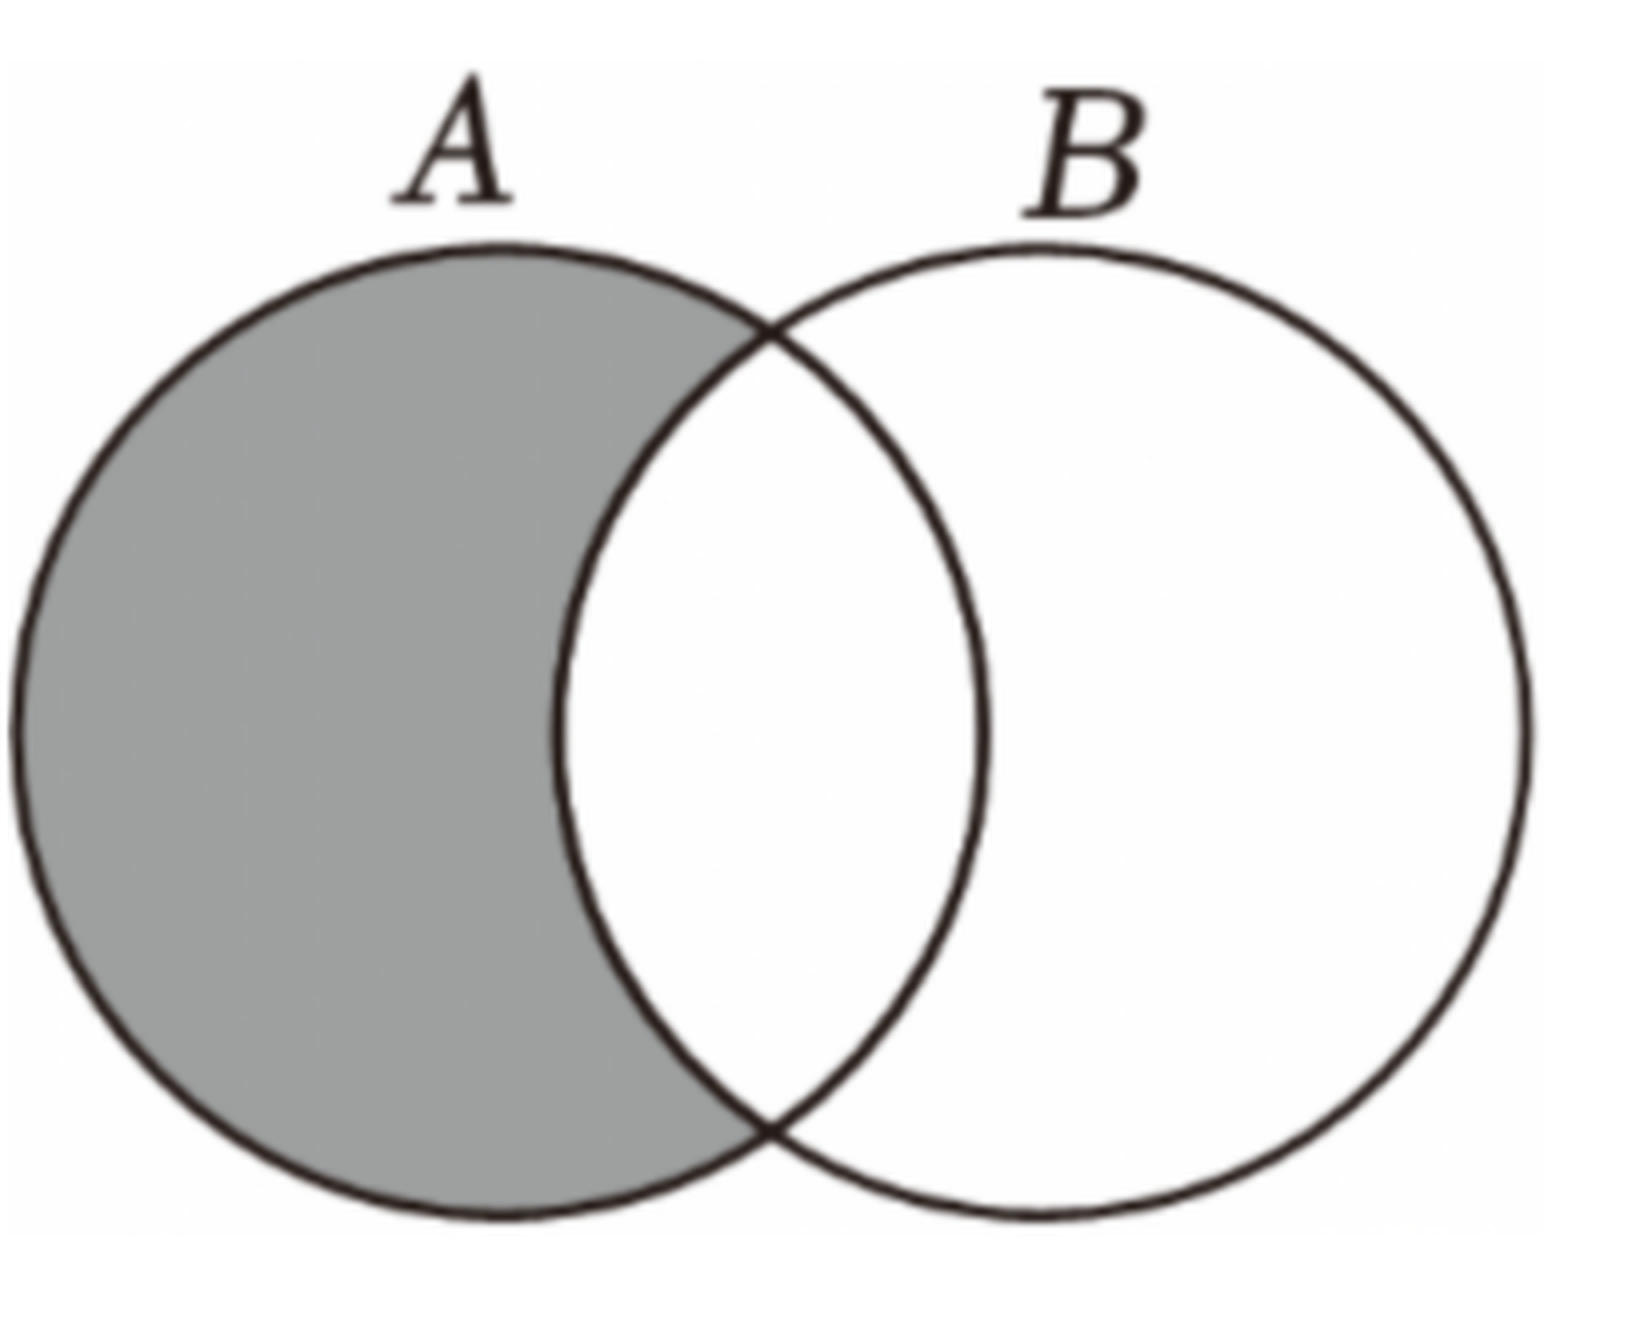
\includegraphics[width=0.30\textwidth]{figures/venn_A_minus_B_h38.png}
\end{center}

\ans{$\{1\}$}

\item 集合 $\{2,3,4,\cdots,2024,2025\}$ 的真子集的个数为 \blankline[4.4em].

\ans{$2^{2024}-1$}

\ifanswer
\solbegin
\step{集合 $\{2,3,4,\cdots,2024,2025\}$ 的真子集的个数为 $2^{2024}-1$.}
\solend

\fi

\item 已知集合 $A$ 中的元素都是正整数，其中最小的是 $1$，最大值是 $100$，除 $1$ 以外，每一个元
素都等于 $A$ 中的两个数（可以相同）的和，则集合 $A$ 中至少含有 \blankline[4.4em] 个元素.

\ans{$9$}

\ifanswer
\solbegin
\step{设 $A$ 中的数从小到大排列为 $1,a_1,a_2,\cdots,a_k,100$，}
\step{则 $a_1=1+1=2$；$3\leqslant a_2\leqslant 4$；$4\leqslant a_3\leqslant 8$；$5\leqslant a_4\leqslant 16$；$6\leqslant a_5\leqslant 32$；$7\leqslant a_6\leqslant 64$；}
\step{于是 $A$ 至少有八个数；}
\step{假设 $A$ 恰好有八个元素，由于 $a_5+a_6\leqslant 96<100$；}
\step{故必须有 $100=a_6+a_6$，$a_6=50$，}
\step{又 $a_4+a_5\leqslant 48$，同理 $a_5=25$，}
\step{但此时 $a_3+a_4\leqslant 24$，$a_5=2a_4$，$a_4=12.5$ 矛盾，}
\step{故 $A$ 不可能恰好有八个元素，因此 $A$ 至少有九个元素.}
\step{其九个数可以为 $1$，$2$，$3$，$6$，$12$，$13$，$25$，$50$，$100$.}
\solend

\fi

\item 已知集合 $\{x_1,x_2,x_3,x_4,x_5,x_6\}=\{1,2,3,4,5,6\}$，将 $x_i$ 与 $x_j$（其中 $i\in\{1,2,3\}$，
$j\in\{4,5,6\}$）的乘积 $x_ix_j$ 放入如图的 $3\times3$ 方格中，则方格中全部数之和的最大值为 \blankline[4.4em].

% 原卷的 $3\times3$ 方格是表格式内容（三行三列的公式），本稿按 高一03 的成例用 tabular 排出。
\begin{center}
\begin{tabular}{|c|c|c|}
\hline
$x_1x_4$ & $x_1x_5$ & $x_1x_6$ \\
\hline
$x_2x_4$ & $x_2x_5$ & $x_2x_6$ \\
\hline
$x_3x_4$ & $x_3x_5$ & $x_3x_6$ \\
\hline
\end{tabular}
\end{center}

\ans{$110$}

\ifanswer
\solbegin
\step{由表格数据得所有数之和为}
\step{$S=x_1x_4+x_1x_5+x_1x_6+x_2x_4+x_2x_5+x_2x_6+x_3x_4+x_3x_5+x_3x_6$，}
\step{所以 $S=(x_1+x_2+x_3)(x_4+x_5+x_6)$，}
\step{因为集合 $\{x_1,x_2,x_3,x_4,x_5,x_6\}=\{1,2,3,4,5,6\}$，}
\step{所以 $x_1+x_2+x_3+x_4+x_5+x_6=1+2+3+4+5+6=21$，}
\step{设 $t=x_1+x_2+x_3$，则 $6\leqslant t\leqslant 15$，$t\in\N^*$，}
\step{$S=t(21-t)=-\left(t-\dfrac{21}{2}\right)^2+\dfrac{441}{4}$，}
\step{当 $t=10$ 或 $t=11$ 时，$S=t(21-t)$ 取最大值，最大值为 $110$，}
\step{此时 $\{x_1,x_2,x_3\}=\{1,4,5\}$，$t=10$，所以可取最大值 $110$.}
\solend

\fi

\item 若 $[x]$ 表示不大于 $x$ 的最大整数，方程 $x^2-8[x]+7=0$ 的解集为 \blankline[4.4em].

\ans{$\{1,\sqrt{33},\sqrt{41},7\}$}

\ifanswer
\solbegin
\step{由题意，$x\geqslant[x]=\dfrac{x^2+7}{8}>0$，得 $x^2-8x+7\leqslant 0$，解得 $1\leqslant x\leqslant 7$，}
\step{$[x]=1$，$x^2=1$，$x=1$；}
\step{$[x]=2$，$x^2=9$，$x=3$ 与 $[x]=2$ 矛盾；}
\step{$[x]=3$，$x^2=17$，$x=\sqrt{17}$，$[x]=4$ 与 $[x]=3$ 矛盾；}
\step{$[x]=4$，$x^2=25$，$x=5$ 与 $[x]=4$ 矛盾；}
\step{$[x]=5$，$x^2=33$，$x=\sqrt{33}$，$[x]=5$；}
\step{$[x]=6$，$x^2=41$，$x=\sqrt{41}$，$[x]=6$；}
\step{$[x]=7$，$x^2=49$，$x=7$；}
\step{综上，方程 $x^2-8[x]+7=0$ 的解集为 $\{1,\sqrt{33},\sqrt{41},7\}$.}
\solend

\fi

\end{enumerate}

\bigsec{二、选择题}

\begin{enumerate}
\setcounter{enumi}{10}

\item 已知集合 $A=\{a,a^2\}$，$B=\{1,3\}$，若 $1\in A$，则 $A\cup B$ 中所有元素之和为\mbox{（\quad）}

\keepwithprev
A. $2$\qquad B. $3$\qquad C. $4$\qquad D. $5$

\ans{$B$}

\ifanswer
\solbegin
\step{因为 $1\in A$，集合 $A=\{a,a^2\}$，所以 $a=1$ 或 $a^2=1$，}
\step{若 $a=1$，则 $a=a^2$，与元素的互异性矛盾；}
\step{若 $a^2=1$，则 $a=1$（舍）或 $a=-1$，故 $A=\{-1,1\}$，$B=\{1,3\}$，}
\step{故 $A\cup B=\{-1,1,3\}$，所以 $A\cup B$ 中所有元素之和为 $-1+1+3=3$. 故选 $B$.}
\solend

\fi

\item 对于实数 $a$、$b$、$c$，下列命题正确的是\mbox{（\quad）}

\keepwithprev
A. 若 $a>b$，则 $ac^2>bc^2$\qquad B. 若 $a>b$，则 $a^2>b^2$

C. 若 $a>b$，则 $a|a|>b|b|$\qquad D. 若 $a>b>c>0$，则 $\dfrac{b}{a-b}<\dfrac{c}{a-c}$

\ans{$C$}

\ifanswer
\solbegin
\step{对于 $A$，若 $a>b$，$c=0$，则 $ac^2=bc^2$，故 $A$ 错误；}
\step{对于 $B$，若 $a>b$，取 $a=-1$，$b=-2$，则 $a^2<b^2$，故 $B$ 错误；}
\step{对于 $C$，若 $a>b>0$ 时，$a|a|-b|b|=a^2-b^2>0$，}
\step{当 $a>0>b$ 时，$a|a|-b|b|=a^2+b^2>0$，}
\step{当 $0>a>b$ 时，$a|a|-b|b|=b^2-a^2=(b-a)(b+a)>0$，}
\step{综上，若 $a>b$，则 $a|a|>b|b|$，故 $C$ 正确；}
\step{对于 $D$，若 $a>b>c>0$，$\dfrac{b}{a-b}-\dfrac{c}{a-c}=\dfrac{ab-bc-ac+bc}{(a-b)(a-c)}=\dfrac{a(b-c)}{(a-b)(a-c)}>0$，}
\step{故 $D$ 错误.}
\step{故选 $C$.}
\solend

\fi

\item 对于正整数集合 $A=\{a_1,a_2,\cdots,a_n\}(n\in\N^*,\ n\geqslant 3)$，如果去掉其中任意一个元素
$a_i(i=1,2,\cdots,n)$ 之后，剩余的所有元素组成的集合都能分为两个交集为空集的集合，且这
两个集合的所有元素之和相等，就称集合 $A$ 为平衡集. 记 $M=a_1+a_2+\cdots+a_n$. 若集合 $A$
是平衡集，并且存在 $a_i$ 为奇数，则集合 $A$ 中元素个数 $n$ 的奇偶性\mbox{（\quad）}

\keepwithprev
A. 与 $M$ 相关，既可以是奇数，又可以是偶数

B. 与 $M$ 无关，既可以是奇数，又可以是偶数

C. 与 $M$ 无关，必为偶数

D. 与 $M$ 无关，必为奇数

\ans{$D$}

\ifanswer
\solbegin
\step{正整数集合 $A=\{a_1,a_2,\cdots,a_n\}(n\in\N^*,\ n\geqslant 3)$，}
\step{因为集合 $A$ 是平衡集，设去掉元素 $a_i(i=1,2,\cdots,n)$，}
\step{由题意得 $A=A_1\cup A_2\cup\{a_i\}$，其中 $A_1\cap A_2=\varnothing$，}
\step{设集合 $A_1$ 和 $A_2$ 中的元素之和均为 $m$，所以 $M=2m+a_i$，其中 $i=1,2,\cdots,n$，}
\step{所以 $M-a_i=2m$，所以 $M-a_i$ 为偶数，其中 $i=1,2,\cdots,n$，}
\step{所以 $a_i(i=1,2,\cdots,n)$ 的奇偶性相同；}
\step{因为存在 $a_i$ 为奇数，所以 $a_i(i=1,2,\cdots,n)$ 均为奇数，}
\step{由 $M-a_i=2m$ 得 $M$ 也为奇数，且 $M=a_1+a_2+\cdots+a_n$，}
\step{所以 $n$ 也为奇数，所以 $n$ 必为奇数. 故选 $D$.}
\solend

\fi

\item 对于集合 $M=\{a\mid a=x^2-y^2,\ x\in\Z,\ y\in\Z\}$，给出如下三个结论：其中正确结论的个数
是\mbox{（\quad）}

\keepwithprev
①如果 $P=\{b\mid b=2n+1,\ n\in\Z\}$，那么 $P\sub M$；

②如果 $c=4n+2$，$n\in\Z$，那么 $c\notin M$；

③如果 $a_1\in M$，$a_2\in M$，那么 $a_1a_2\in M$.

\keepwithprev
A. $1$\qquad B. $2$\qquad C. $3$\qquad D. $0$

\ans{$C$}

\ifanswer
\solbegin
\step{对于①，$b=2n+1$，$n\in\Z$，则恒有 $2n+1=(n+1)^2-n^2$，}
\step{所以 $2n+1\in M$，即 $P=\{b\mid b=2n+1,n\in\Z\}$，则 $P\sub M$，①正确；}
\step{对于②，$c=4n+2$，$n\in\Z$，}
\step{若 $4n+2\in M$，则存在 $x$、$y\in\Z$ 使得 $x^2-y^2=4n+2$，}
\step{所以 $4n+2=(x+y)(x-y)$，又 $x+y$ 和 $x-y$ 同奇或同偶，}
\step{若 $x+y$ 和 $x-y$ 都是奇数，则 $(x+y)(x-y)$ 为奇数，而 $4n+2$ 是偶数；}
\step{若 $x+y$ 和 $x-y$ 都是偶数，则 $(x+y)(x-y)$ 能被 $4$ 整除，而 $4n+2$ 不能被 $4$ 整除，}
\step{所以 $4n+2\notin M$，即 $c\notin M$，②正确；}
\step{对于③，$a_1\in M$，$a_2\in M$，可设 $a_1=x_1^2-y_1^2$，$a_2=x_2^2-y_2^2$，$x_i$、$y_i\in\Z$；}
\step{则 $a_1a_2=(x_1^2-y_1^2)(x_2^2-y_2^2)=(x_1x_2)^2+(y_1y_2)^2-(x_1y_2)^2-(x_2y_1)^2$}
\step{$=(x_1x_2+y_1y_2)^2-(x_1y_2+x_2y_1)^2\in M$，那么 $a_1a_2\in M$，③正确.}
\step{综上，正确的命题是①②③. 故选 $C$.}
\solend

\fi

\end{enumerate}

\bigsec{三、解答题}

\begin{enumerate}
\setcounter{enumi}{14}

\item 已知 $A=\{x\mid a\leqslant x\leqslant -a+3\}$，$B=\{x\mid x<-1\text{ 或 }x>5\}$.

\begin{enumerate}[label=(\arabic*)]

\item 若 $A\cap B=\varnothing$，求 $a$ 的取值范围；

\item 若 $A\cup B=\R$，求 $a$ 的取值范围.

\end{enumerate}

\ans{（1）$[-1,+\infty)$；（2）$(-\infty,-2]$}

\ifanswer
\solbegin
\stepm{(1)}{①当 $A=\varnothing$ 时，$A\cap B=\varnothing$，需满足 $a>-a+3$，解得 $a>\dfrac32$，}
\step{故 $a$ 的取值范围为 $\left(\dfrac32,+\infty\right)$.}
\step{②当 $A\neq\varnothing$ 时，要使 $A\cap B=\varnothing$，需满足
$\begin{cases}a\leqslant\dfrac32\\[4pt] -a+3\leqslant 5\\[4pt] a\geqslant -1\end{cases}$，解得 $-1\leqslant a\leqslant\dfrac32$.}
\step{综上所述，$a$ 的取值范围是 $[-1,+\infty)$.}
\stepm{(2)}{因为 $A\cup B=\R$，$A=\{x\mid a\leqslant x\leqslant -a+3\}$，$B=\{x\mid x<-1\text{ 或 }x>5\}$，}
\step{所以 $\begin{cases}-a+3\geqslant 5\\[4pt] a\leqslant -1\end{cases}$，解得 $a\leqslant -2$，故所求 $a$ 的取值范围为 $(-\infty,-2]$.}
\solend

\fi

\ansspace[6]

\item 已知集合 $A=\{x\mid mx^2+x-2=0\}$，$B=\{x\mid 2x^2-5x-12=0\}$.

\begin{enumerate}[label=(\arabic*)]

\item 若 $A$ 中有且仅有 $1$ 个元素，求实数 $m$ 的值；

\item 已知集合 $C=A\cup B$，若 $C$ 的真子集有且仅有 $3$ 个，求实数 $m$ 的取值范围.

\end{enumerate}

\ans{（1）$m=0$ 或 $m=-\dfrac18$；（2）$\left\{m\mid m\leqslant -\dfrac18\right\}$}

\ifanswer
\solbegin
\stepm{(1)}{若 $m=0$，方程化为 $x-2=0$，此时方程有且仅有一个根 $x=2$；}
\step{若 $m\neq 0$，则 $\Delta=1^2-4\times m\times(-2)=0$，即 $m=-\dfrac18$ 时，}
\step{方程有两个相等的实根，此时集合 $A$ 中有且仅有一个元素，}
\step{所以实数 $m$ 的值为 $m=0$ 或 $m=-\dfrac18$；}
\stepm{(2)}{$B=\{x\mid 2x^2-5x-12=0\}=\left\{-\dfrac32,4\right\}$，}
\step{因为 $C=A\cup B$，若 $C$ 的真子集有且仅有 $3$ 个，则 $C$ 中有两个元素，}
\step{所以 $A\sub B$，由（1）得 $m=0$ 时，$A=\{2\}$，不符合 $A\sub B$，}
\step{当 $m\neq 0$ 时，若 $\Delta=1^2-4\times m\times(-2)<0$，解得 $m<-\dfrac18$，}
\step{此时 $A=\varnothing$，符合 $A\sub B$，}
\step{若 $\Delta=1^2-4\times m\times(-2)=0$，解得 $m=-\dfrac18$，}
\step{此时方程 $mx^2+x-2=0$ 的根为 $x=4$，集合 $A=\{4\}$，符合 $A\sub B$，}
\step{若 $\Delta=1^2-4\times m\times(-2)>0$，由 $A\sub B$，得 $A=\left\{-\dfrac32,4\right\}$，}
\step{此时有 $-\dfrac32+4=-\dfrac1m$ 且 $-\dfrac32\times 4=-\dfrac2m$，无解，}
\step{综上所述，实数 $m$ 的取值范围为 $\left\{m\mid m\leqslant -\dfrac18\right\}$.}
\solend

\fi

\ansspace[6]

\item 设 $A$ 是非空实数集，且 $0\notin A$. 若对于任意的 $x$、$y\in A$，都有 $xy\in A$，则称集合 $A$ 具
有性质 $P_1$；若对于任意的 $x$、$y\in A$，都有 $\dfrac xy\in A$，则称集合 $A$ 具有性质 $P_2$.

\begin{enumerate}[label=(\arabic*)]

\item 写出一个恰含有两个元素且具有性质 $P_1$ 的集合 $A$，并说明理由；

\item 证明：“非空实数集 $A$ 具有性质 $P_1$”是“非空实数集 $A$ 具有性质 $P_2$”的必要非充分条
件.

\end{enumerate}

\ans{（1）$A=\{-1,1\}$，理由见解析；（2）见解析}

\ifanswer
\solbegin
% 注：原卷本题 (1) 的解析里“证明”一词重复出现两次（一次接在分号后、一次另起一行），
%     本稿照原卷重复录入，未去重。
\stepm{(1)}{$A=\{-1,1\}$，证明：恰含有两个元素且具有性质 $P_1$ 的集合 $A=\{-1,1\}$；}
\step{证明：$1\times 1=1\in A$，$1\times(-1)=-1\in A$，$-1\times 1=-1\in A$，$-1\times(-1)=1\in A$；}
\stepm{(2)}{若集合 $A$ 具有性质 $P_2$，不妨设 $a\in A$，}
\step{由非空数集 $A$ 具有性质 $P_2$，有 $\dfrac aa=1\in A$.}
\step{①$A=\{1\}$，易得此时集合 $A$ 具有性质 $P_1$.}
\step{②数集 $A$ 只含有两个元素，不妨设 $A=\{1,a_1\}$，}
\step{由 $\dfrac{1}{a_1}=a_1$，且 $a_1\neq 1$，解得 $a_1=-1$，此时集合 $A$ 具有性质 $P_1$.}
\step{③实数集 $A$ 含有两个以上的元素，不妨设不为 $1$ 的元素 $a_1$、$a_2\in A$，}
\step{则有 $\dfrac{1}{a_1}\in A$，由于集合 $A$ 具有性质 $P_2$，}
\step{所以有 $a_2\div\dfrac{1}{a_1}=a_1a_2\in A$，这说明集合 $A$ 具有性质 $P_1$.}
\step{综上，若非空实数集 $A$ 具有性质 $P_2$，则集合 $A$ 具有性质 $P_1$，}
\step{所以“非空实数集 $A$ 具有性质 $P_1$”是“非空实数集 $A$ 具有性质 $P_2$”的}
\step{必要条件.}
\step{取正偶数集 $A=\{x\mid x=2n,\ n\in\N^*\}$，}
\step{对任意的 $2m$、$2n\in A$，$m$、$n\in\N^*$，}
\step{有 $2m\times 2n=4mn\in A$，故 $A$ 具有性质 $P_1$，}
\step{取 $x=2$，$y=4$，则 $\dfrac xy=\dfrac12\notin A$，故 $A$ 不具有性质 $P_2$，}
\step{所以“非空实数集 $A$ 具有性质 $P_1$”不是“非空实数集 $A$ 具有性质 $P_2$”的}
\step{充分条件.}
\step{综上，“非空实数集 $A$ 具有性质 $P_1$”是“非空实数集 $A$ 具有性质 $P_2$”的}
\step{必要非充分条件.}
\solend

\fi

\ansspace[8]

\item 已知命题 $p$：关于 $x$ 的方程 $x^2+mx+1=0$ 有两个不同的正根；命题 $q$：关于 $x$ 的方程
$4x^2+4(m-2)x=-1$ 有实根.

\begin{enumerate}[label=(\arabic*)]

\item 若命题 $q$ 为假命题，求整数 $m$ 的解集；

\item 若命题 $p$ 为真命题，且关于 $x$ 的方程 $x^2+mx+1=0$ 的两个实数根 $x_1$、$x_2$ 满足
$3x_1+2x_2=5$，求实数 $m$ 的取值集合；

\item 若命题 $p$ 和命题 $q$ 有且仅有一个成立，求实数 $m$ 的取值范围.

\end{enumerate}

\ans{（1）$\{2\}$；（2）$\left\{-\dfrac{13}{6}\right\}$；（3）$[-2,1]\cup[3,+\infty)$}

\ifanswer
\solbegin
\stepm{(1)}{命题 $q$：关于 $x$ 的方程 $4x^2+4(m-2)x=-1$ 有实根为假命题，}
\step{即 $4x^2+4(m-2)x+1=0$ 无实根，}
\step{则 $\Delta=16(m-2)^2-16<0$，则 $1<m<3$，则整数 $m$ 的解集为 $\{2\}$；}
\stepm{(2)}{若命题 $p$ 为真命题，且关于 $x$ 的方程 $x^2+mx+1=0$ 的两个实数根 $x_1$、$x_2$，}
\step{满足 $3x_1+2x_2=5$，则方程 $x^2+mx+1=0$ 有两个不同的正根，}
\step{则 $\begin{cases}\Delta=m^2-4>0\\[4pt] x_1+x_2=-m>0\end{cases}$，则 $m<-2$，}
\step{又 $\begin{cases}x_1+x_2=-m\\[4pt] x_1x_2=1\\[4pt] 3x_1+2x_2=5\end{cases}$，
则 $\begin{cases}x_1=5+2m\\[4pt] x_2=-3m-5\end{cases}$，则 $(5+2m)(-3m-5)=1$，}
\step{得 $m=-2$ 或 $m=-\dfrac{13}{6}$，又因为 $m<-2$，所以 $m=-\dfrac{13}{6}$，}
\step{所以实数 $m$ 的取值集合为 $\left\{-\dfrac{13}{6}\right\}$；}
\stepm{(3)}{由（2）得当 $p$ 为真时，则有 $m<-2$，}
\step{当 $q$ 为真时，$\Delta=16(m-2)^2-16\geqslant 0$，解得 $m\leqslant 1$ 或 $m\geqslant 3$，}
\step{又因为命题 $p$ 和命题 $q$ 只有一个为真，所以
$\begin{cases}m<-2\\[4pt] 1<m<3\end{cases}$ 或 $\begin{cases}m\geqslant -2\\[4pt] m\leqslant 1\text{ 或 }m\geqslant 3\end{cases}$，}
\step{解得 $-2\leqslant m\leqslant 1$ 或 $m\geqslant 3$，所以实数 $m$ 的取值范围为 $[-2,1]\cup[3,+\infty)$.}
\solend

\fi

\ansspace[8]

% 注：原卷此处作“设 $n\in\N^*$，集合含有 $3n$ 个元素”，**漏了符号 $U$**（应作“集合 $U$
%     含有 $3n$ 个元素”）——$U$ 直到本句末尾“则称 $U$ 为三分集合”才出现、此前无定义。
%     本稿照录未补，见文件头“原卷笔误/存疑”⑦。
\item 设 $n\in\N^*$，集合含有 $3n$ 个元素，若存在三个 $n$ 元集合 $A$、$B$、$C$ 满足如下两个条件，
则称 $U$ 为三分集合.

①$U=A\cup B\cup C$；

②$A$、$B$、$C$ 元素可分别排列为有序数组 $(a_1,a_2,\cdots,a_n)$，$(b_1,b_2,\cdots,b_n)$ 及
$(c_1,c_2,\cdots,c_n)$，使得对 $\forall i=1,2,\cdots,n$，均有 $a_i+b_i=c_i$.

特别地，当 $U=\{1,2,3,4,\cdots,3n-2,3n-1,3n\}$ 为三分集合时，称 $n$ 为完美三分数.

如：因为 $U=\{1,2,3\}$ 为三分集合，所以 $n=1$ 为最小完美三分数.

\begin{enumerate}[label=(\arabic*)]

\item 请判断下列两个集合是否为三分集合（直接写出结论）：

$U_1=\{1,2,3,4,5,6\}$，$U_2=\{1,3,5,7,8,9,10,11,12\}$；

\item 求出大于 $1$ 的最小完美三分数；

\item 请判断是否存在无穷多个完美三分数？若存在，请说明理由；若不存在，则求出最大的
完美三分数.

\end{enumerate}

\ans{（1）$U_1$ 不是三分集合，$U_2$ 是三分集合；（2）$4$；（3）存在，理由见解析}

\ifanswer
\solbegin
\stepm{(1)}{(i)$U_1=\{1,2,3,4,5,6\}$ 不是三分集合，下面用反证法证明：}
\step{证明：假设 $U=\{1,2,3,4,5,6\}$ 是三分集合，}
\step{设 $A=\{a_1,a_2\}$，$B=\{b_1,b_2\}$，$C=\{c_1,c_2\}$，不妨设 $c_1<c_2$，}
\step{因为 $a_1+b_1=c_1$，$a_2+b_2=c_2$，}
\step{所以 $a_1+b_1+a_2+b_2+c_1+c_2=2(c_1+c_2)=1+2+3+4+5+6=21$，}
% 注：原卷此步印“所以 $c_1+c_2=2$”，与上一行的 $2(c_1+c_2)=21$ **不自洽**
%     （应作 $\dfrac{21}2$）；同题 $n=3$ 处的同型推理原卷写的是 $\dfrac{45}2$，故此处是原卷笔误。
%     本稿照录未改，见文件头“原卷笔误/存疑”⑧。
\step{所以 $c_1+c_2=2$，这与 $c_1,c_2\in\N^*$ 矛盾，故假设错误，}
\step{故 $U_1=\{1,2,3,4,5,6\}$ 不是三分集合；}
\step{(ii)$U_2=\{1,3,5,7,8,9,10,11,12\}$ 是三分集合，理由如下：}
\step{令 $A=\{1,3,5\}$，$B=\{9,8,7\}$，$C=\{10,11,12\}$，}
\step{则 $A\cup B\cup C=U=\{1,3,5,7,8,9,10,11,12\}$，满足条件①；}
\step{又 $1+9=10$；$3+8=11$；$5+7=12$，所以满足条件②，}
\step{所以 $U_2=\{1,3,5,7,8,9,10,11,12\}$ 是三分集合；}
\stepm{(2)}{由（1）得，当 $n=2$ 时，$U=\{1,2,3,4,5,6\}$ 不是三分集合；}
\step{当 $n=3$ 时，$U=\{1,2,3,4,5,6,7,8,9\}$，}
\step{假设 $U=\{1,2,3,4,5,6,7,8,9\}$ 是三分集合，}
\step{同理由 $a_1+b_1+a_2+b_2+a_3+b_3+c_1+c_2+c_3$}
\step{$=2(c_1+c_2+c_3)=1+2+\cdots+9=45$，$c_1+c_2+c_3=\dfrac{45}{2}$，}
\step{可推出与 $c_1$、$c_2$、$c_3\in\N^*$ 矛盾，故假设也错误，}
\step{所以 $U=\{1,2,3,4,5,6,7,8,9\}$ 不是三分集合；}
\step{当 $n=4$ 时，$U=\{1,2,3,\cdots,12\}$，}
\step{存在三个 $4$ 元集合 $A=\{1,2,4,3\}$，$B=\{5,8,7,9\}$，$C=\{6,10,11,12\}$，}
\step{满足 $U=\{1,2,3,\cdots,12\}$ 为三分集合的两个条件，}
\step{故大于 $1$ 的最小完美三分数为 $4$；}
\stepm{(3)}{存在无穷多个完美三分数，理由如下：}
\step{由题意得，$n=1$ 为最小完美三分数，}
\step{当 $n=5$ 时，$U=\{1,2,3,\cdots,15\}$，}
\step{存在三个 $5$ 元集合 $A=\{1,3,5,7,2\}$，$B=\{11,10,9,8,4\}$，$C=\{12,13,14,15,6\}$，}
\step{满足三分集合的条件，故 $5$ 为完美三分数；}
\step{当 $n=21$ 时，$U=\{1,2,3,\cdots,63\}$，}
\step{存在如下三个 $21$ 元的集合满足三分集合的条件：}
\step{$A=\{1,3,5,7,\cdots,29,31,2,6,10,14,4\}$，}
\step{$B=\{47,46,45,44,\cdots,33,32,22,20,18,16,8\}$，}
\step{$C=\{48,49,50,51,\cdots,62,63,24,26,28,30,12\}$，}
\step{故 $21$ 为完美三分数.}
\step{首先证明：若 $n=k$，$k\in\N^*$ 为三分完美数，}
\step{则 $n=4k+1$，$k\in\N^*$ 也为三分完美数，}
% 注：下一行原卷印作“$U_{k+1}=U_{k+1}=\{2,3,\cdots,12k+3\}$”——等号两边记号相同，
%     依上下文疑当作 $U'_{k+1}=U_{4k+1}$，且此处集合自 2 起（前文 $U_{4k+1}$ 自 1 起）；
%     本稿照录原卷，未代为改写。
\step{证明：记 $U_k=\{1,2,3,\cdots,3k\}$，$U_{4k+1}=\{1,2,3,\cdots,12k+3\}$，}
\step{若 $n=k$，$k\in\N^*$ 为三分完美数，则 $U_k$ 为三分集合，}
\step{即存在三个 $k$ 元集合 $A$、$B$、$C$ 满足如下两个条件，}
\step{①$U_k=A\cup B\cup C$；}
\step{②$A$、$B$、$C$ 元素可分别排列为有序数组 $(a_1,a_2,\cdots,a_k)$，}
\step{$(b_1,b_2,\cdots,b_k)$ 及 $(c_1,c_2,\cdots,c_k)$，}
\step{使得对 $\forall i=1,2,3,\cdots,k$，均有 $a_i+b_i=c_i$，}
\step{则可得到对 $\forall i=1,2,3,\cdots,k$，$2a_i+2b_i=2c_i$，}
\step{故集合 $\{2,4,6,\cdots,6k\}$ 也满足三分集合的两个条件，其也为三分集合，}
\step{下面记集合 $\{2,4,6,\cdots,6k\}=2U_k$，}
\step{对 $n=4k+1$，集合 $U_{k+1}=U_{k+1}=\{2,3,\cdots,12k+3\}=(2U_k)\cup\complement_{U_{4k+1}}(2U_k)$，}
\step{构造集合 $A'=\{1,3,5,7,\cdots,6k+1\}$，共有 $3k+1$ 个奇数；}
% 注：下一行原卷印作“$B'=\{6k+3k+2,6k+3k+1,6k+3k,6k+3k-1,\cdots,6k+2\}$”，
%     按与后文 $C'$ 相接，前四项当写作 $9k+2$、$9k+1$、$9k$、$9k-1$；本稿照录原卷。
\step{集合 $B'=\{6k+3k+2,6k+3k+1,6k+3k,6k+3k-1,\cdots,6k+2\}$，}
\step{共有 $3k+1$ 个逐个减小的连续正整数；}
\step{集合 $C'=\{9k+3,9k+4,9k+5,9k+6,\cdots,12k+3\}$，}
\step{共有 $3k+1$ 个逐个增大的连续正整数；}
\step{得这三个 $3k+1$ 元集合 $A'$、$B'$、$C'$ 满足如下两个条件，}
\step{①集合 $A'\cup B'\cup C'=\complement_{U_{4k+1}}(2U_k)$；}
\step{②$A'$、$B'$、$C'$ 元素可分别排列为有序数组 $(a_1,a_2,\cdots,a_{3k+1})$，}
\step{$(b_1,b_2,\cdots,b_{3k+1})$ 及 $(c_1,c_2,\cdots,c_{3k+1})$，}
\step{使得对 $\forall i=1,2,3,\cdots,3k+1$，均有 $a_i+b_i=c_i$；}
\step{故 $\complement_{U_{4k+1}}(2U_k)$ 为三分集合，而已知 $U_k$ 为三分集合，}
\step{将其对应与 $A'$、$B'$、$C'$ 合并，}
% 注：原卷此处印“令 $A''=A\cup A'$”（$B''$、$C''$ 同）。按同段上文“记集合
%     $\{2,4,6,\cdots,6k\}=2U_k$”，此处疑当作 $A''=2A\cup A'$——否则
%     $A''\cup B''\cup C''=U_k\cup\complement_{U_{4k+1}}(2U_k)\neq U_{4k+1}$，与本段结论冲突。
%     本稿照录未改，见文件头“原卷笔误/存疑”⑨。
\step{令 $A''=A\cup A'$，$B''=B\cup B'$，$C''=C\cup C'$，}
\step{则这三个 $4k+1$ 元集合 $A''$、$B''$、$C''$，}
\step{满足 $A''\cup B''\cup C''=U_{4k+1}$，且满足条件②，}
\step{故 $U_{4k+1}=\{1,2,3,\cdots,12k+3\}$ 为三分集合，}
\step{因此可得，若 $n=k$ 为三分完美数，则 $n=4k+1$ 也为三分完美数，}
\step{由 $1$，$5$，$21$ 为完美三分数，结合所证结论得，存在无穷多个完美三分数.}
\solend

\fi

\ansspace*[12]

\end{enumerate}

\end{document}
